\documentclass[twoside]{book}

% Packages required by doxygen
\usepackage{fixltx2e}
\usepackage{calc}
\usepackage{doxygen}
\usepackage[export]{adjustbox} % also loads graphicx
\usepackage{graphicx}
\usepackage[utf8]{inputenc}
\usepackage{makeidx}
\usepackage{multicol}
\usepackage{multirow}
\PassOptionsToPackage{warn}{textcomp}
\usepackage{textcomp}
\usepackage[nointegrals]{wasysym}
\usepackage[table]{xcolor}

% Font selection
\usepackage[T1]{fontenc}
\usepackage[scaled=.90]{helvet}
\usepackage{courier}
\usepackage{amssymb}
\usepackage{sectsty}
\renewcommand{\familydefault}{\sfdefault}
\allsectionsfont{%
  \fontseries{bc}\selectfont%
  \color{darkgray}%
}
\renewcommand{\DoxyLabelFont}{%
  \fontseries{bc}\selectfont%
  \color{darkgray}%
}
\newcommand{\+}{\discretionary{\mbox{\scriptsize$\hookleftarrow$}}{}{}}

% Page & text layout
\usepackage{geometry}
\geometry{%
  a4paper,%
  top=2.5cm,%
  bottom=2.5cm,%
  left=2.5cm,%
  right=2.5cm%
}
\tolerance=750
\hfuzz=15pt
\hbadness=750
\setlength{\emergencystretch}{15pt}
\setlength{\parindent}{0cm}
\setlength{\parskip}{3ex plus 2ex minus 2ex}
\makeatletter
\renewcommand{\paragraph}{%
  \@startsection{paragraph}{4}{0ex}{-1.0ex}{1.0ex}{%
    \normalfont\normalsize\bfseries\SS@parafont%
  }%
}
\renewcommand{\subparagraph}{%
  \@startsection{subparagraph}{5}{0ex}{-1.0ex}{1.0ex}{%
    \normalfont\normalsize\bfseries\SS@subparafont%
  }%
}
\makeatother

% Headers & footers
\usepackage{fancyhdr}
\pagestyle{fancyplain}
\fancyhead[LE]{\fancyplain{}{\bfseries\thepage}}
\fancyhead[CE]{\fancyplain{}{}}
\fancyhead[RE]{\fancyplain{}{\bfseries\leftmark}}
\fancyhead[LO]{\fancyplain{}{\bfseries\rightmark}}
\fancyhead[CO]{\fancyplain{}{}}
\fancyhead[RO]{\fancyplain{}{\bfseries\thepage}}
\fancyfoot[LE]{\fancyplain{}{}}
\fancyfoot[CE]{\fancyplain{}{}}
\fancyfoot[RE]{\fancyplain{}{\bfseries\scriptsize Generated by Doxygen }}
\fancyfoot[LO]{\fancyplain{}{\bfseries\scriptsize Generated by Doxygen }}
\fancyfoot[CO]{\fancyplain{}{}}
\fancyfoot[RO]{\fancyplain{}{}}
\renewcommand{\footrulewidth}{0.4pt}
\renewcommand{\chaptermark}[1]{%
  \markboth{#1}{}%
}
\renewcommand{\sectionmark}[1]{%
  \markright{\thesection\ #1}%
}

% Indices & bibliography
\usepackage{natbib}
\usepackage[titles]{tocloft}
\setcounter{tocdepth}{3}
\setcounter{secnumdepth}{5}
\makeindex

% Hyperlinks (required, but should be loaded last)
\usepackage{ifpdf}
\ifpdf
  \usepackage[pdftex,pagebackref=true]{hyperref}
\else
  \usepackage[ps2pdf,pagebackref=true]{hyperref}
\fi
\hypersetup{%
  colorlinks=true,%
  linkcolor=blue,%
  citecolor=blue,%
  unicode%
}

% Custom commands
\newcommand{\clearemptydoublepage}{%
  \newpage{\pagestyle{empty}\cleardoublepage}%
}

\usepackage{caption}
\captionsetup{labelsep=space,justification=centering,font={bf},singlelinecheck=off,skip=4pt,position=top}

%===== C O N T E N T S =====

\begin{document}

% Titlepage & ToC
\hypersetup{pageanchor=false,
             bookmarksnumbered=true,
             pdfencoding=unicode
            }
\pagenumbering{alph}
\begin{titlepage}
\vspace*{7cm}
\begin{center}%
{\Large reactor-\/cpp }\\
\vspace*{1cm}
{\large Generated by Doxygen 1.8.13}\\
\end{center}
\end{titlepage}
\clearemptydoublepage
\pagenumbering{roman}
\tableofcontents
\clearemptydoublepage
\pagenumbering{arabic}
\hypersetup{pageanchor=true}

%--- Begin generated contents ---
\chapter{Namespace Index}
\section{Namespace List}
Here is a list of all namespaces with brief descriptions\+:\begin{DoxyCompactList}
\item\contentsline{section}{\hyperlink{namespacereactor}{reactor} }{\pageref{namespacereactor}}{}
\item\contentsline{section}{\hyperlink{namespacereactor_1_1log}{reactor\+::log} }{\pageref{namespacereactor_1_1log}}{}
\item\contentsline{section}{\hyperlink{namespacereactor_1_1operators}{reactor\+::operators} }{\pageref{namespacereactor_1_1operators}}{}
\end{DoxyCompactList}

\chapter{Hierarchical Index}
\section{Class Hierarchy}
This inheritance list is sorted roughly, but not completely, alphabetically\+:\begin{DoxyCompactList}
\item \contentsline{section}{reactor\+:\+:log\+:\+:Base\+Logger$<$ enabled $>$}{\pageref{classreactor_1_1log_1_1BaseLogger}}{}
\item \contentsline{section}{reactor\+:\+:log\+:\+:Base\+Logger$<$ debug\+\_\+enabled $>$}{\pageref{classreactor_1_1log_1_1BaseLogger}}{}
\begin{DoxyCompactList}
\item \contentsline{section}{reactor\+:\+:log\+:\+:Debug}{\pageref{structreactor_1_1log_1_1Debug}}{}
\end{DoxyCompactList}
\item \contentsline{section}{reactor\+:\+:log\+:\+:Base\+Logger$<$ error\+\_\+enabled $>$}{\pageref{classreactor_1_1log_1_1BaseLogger}}{}
\begin{DoxyCompactList}
\item \contentsline{section}{reactor\+:\+:log\+:\+:Error}{\pageref{structreactor_1_1log_1_1Error}}{}
\end{DoxyCompactList}
\item \contentsline{section}{reactor\+:\+:log\+:\+:Base\+Logger$<$ false $>$}{\pageref{classreactor_1_1log_1_1BaseLogger_3_01false_01_4}}{}
\item \contentsline{section}{reactor\+:\+:log\+:\+:Base\+Logger$<$ info\+\_\+enabled $>$}{\pageref{classreactor_1_1log_1_1BaseLogger}}{}
\begin{DoxyCompactList}
\item \contentsline{section}{reactor\+:\+:log\+:\+:Info}{\pageref{structreactor_1_1log_1_1Info}}{}
\end{DoxyCompactList}
\item \contentsline{section}{reactor\+:\+:log\+:\+:Base\+Logger$<$ true $>$}{\pageref{classreactor_1_1log_1_1BaseLogger_3_01true_01_4}}{}
\item \contentsline{section}{reactor\+:\+:log\+:\+:Base\+Logger$<$ warning\+\_\+enabled $>$}{\pageref{classreactor_1_1log_1_1BaseLogger}}{}
\begin{DoxyCompactList}
\item \contentsline{section}{reactor\+:\+:log\+:\+:Warn}{\pageref{structreactor_1_1log_1_1Warn}}{}
\end{DoxyCompactList}
\item \contentsline{section}{reactor\+:\+:Environment}{\pageref{classreactor_1_1Environment}}{}
\item \contentsline{section}{reactor\+:\+:Immutable\+Value\+Ptr$<$ T $>$}{\pageref{classreactor_1_1ImmutableValuePtr}}{}
\item \contentsline{section}{reactor\+:\+:Logical\+Time}{\pageref{classreactor_1_1LogicalTime}}{}
\item \contentsline{section}{reactor\+:\+:Mutable\+Value\+Ptr$<$ T $>$}{\pageref{classreactor_1_1MutableValuePtr}}{}
\item \contentsline{section}{reactor\+:\+:Reactor\+Element}{\pageref{classreactor_1_1ReactorElement}}{}
\begin{DoxyCompactList}
\item \contentsline{section}{reactor\+:\+:Base\+Action}{\pageref{classreactor_1_1BaseAction}}{}
\begin{DoxyCompactList}
\item \contentsline{section}{reactor\+:\+:Action$<$ T $>$}{\pageref{classreactor_1_1Action}}{}
\begin{DoxyCompactList}
\item \contentsline{section}{reactor\+:\+:Logical\+Action$<$ T $>$}{\pageref{classreactor_1_1LogicalAction}}{}
\item \contentsline{section}{reactor\+:\+:Physical\+Action$<$ T $>$}{\pageref{classreactor_1_1PhysicalAction}}{}
\end{DoxyCompactList}
\item \contentsline{section}{reactor\+:\+:Action$<$ void $>$}{\pageref{classreactor_1_1Action_3_01void_01_4}}{}
\item \contentsline{section}{reactor\+:\+:Shutdown\+Action}{\pageref{classreactor_1_1ShutdownAction}}{}
\item \contentsline{section}{reactor\+:\+:Timer}{\pageref{classreactor_1_1Timer}}{}
\begin{DoxyCompactList}
\item \contentsline{section}{reactor\+:\+:Startup\+Action}{\pageref{classreactor_1_1StartupAction}}{}
\end{DoxyCompactList}
\end{DoxyCompactList}
\item \contentsline{section}{reactor\+:\+:Base\+Port}{\pageref{classreactor_1_1BasePort}}{}
\begin{DoxyCompactList}
\item \contentsline{section}{reactor\+:\+:Port$<$ T $>$}{\pageref{classreactor_1_1Port}}{}
\begin{DoxyCompactList}
\item \contentsline{section}{reactor\+:\+:Input$<$ T $>$}{\pageref{classreactor_1_1Input}}{}
\item \contentsline{section}{reactor\+:\+:Output$<$ T $>$}{\pageref{classreactor_1_1Output}}{}
\end{DoxyCompactList}
\item \contentsline{section}{reactor\+:\+:Port$<$ void $>$}{\pageref{classreactor_1_1Port_3_01void_01_4}}{}
\end{DoxyCompactList}
\item \contentsline{section}{reactor\+:\+:Reaction}{\pageref{classreactor_1_1Reaction}}{}
\item \contentsline{section}{reactor\+:\+:Reactor}{\pageref{classreactor_1_1Reactor}}{}
\end{DoxyCompactList}
\item runtime\+\_\+error\begin{DoxyCompactList}
\item \contentsline{section}{reactor\+:\+:Validation\+Error}{\pageref{classreactor_1_1ValidationError}}{}
\end{DoxyCompactList}
\item \contentsline{section}{reactor\+:\+:Scheduler}{\pageref{classreactor_1_1Scheduler}}{}
\item \contentsline{section}{reactor\+:\+:Tag}{\pageref{classreactor_1_1Tag}}{}
\end{DoxyCompactList}

\chapter{Class Index}
\section{Class List}
Here are the classes, structs, unions and interfaces with brief descriptions\+:\begin{DoxyCompactList}
\item\contentsline{section}{\hyperlink{classreactor_1_1Action}{reactor\+::\+Action$<$ T $>$} }{\pageref{classreactor_1_1Action}}{}
\item\contentsline{section}{\hyperlink{classreactor_1_1Action_3_01void_01_4}{reactor\+::\+Action$<$ void $>$} }{\pageref{classreactor_1_1Action_3_01void_01_4}}{}
\item\contentsline{section}{\hyperlink{classreactor_1_1BaseAction}{reactor\+::\+Base\+Action} }{\pageref{classreactor_1_1BaseAction}}{}
\item\contentsline{section}{\hyperlink{classreactor_1_1log_1_1BaseLogger}{reactor\+::log\+::\+Base\+Logger$<$ enabled $>$} }{\pageref{classreactor_1_1log_1_1BaseLogger}}{}
\item\contentsline{section}{\hyperlink{classreactor_1_1log_1_1BaseLogger_3_01false_01_4}{reactor\+::log\+::\+Base\+Logger$<$ false $>$} }{\pageref{classreactor_1_1log_1_1BaseLogger_3_01false_01_4}}{}
\item\contentsline{section}{\hyperlink{classreactor_1_1log_1_1BaseLogger_3_01true_01_4}{reactor\+::log\+::\+Base\+Logger$<$ true $>$} }{\pageref{classreactor_1_1log_1_1BaseLogger_3_01true_01_4}}{}
\item\contentsline{section}{\hyperlink{classreactor_1_1BasePort}{reactor\+::\+Base\+Port} }{\pageref{classreactor_1_1BasePort}}{}
\item\contentsline{section}{\hyperlink{structreactor_1_1log_1_1Debug}{reactor\+::log\+::\+Debug} }{\pageref{structreactor_1_1log_1_1Debug}}{}
\item\contentsline{section}{\hyperlink{classreactor_1_1Environment}{reactor\+::\+Environment} }{\pageref{classreactor_1_1Environment}}{}
\item\contentsline{section}{\hyperlink{structreactor_1_1log_1_1Error}{reactor\+::log\+::\+Error} }{\pageref{structreactor_1_1log_1_1Error}}{}
\item\contentsline{section}{\hyperlink{classreactor_1_1ImmutableValuePtr}{reactor\+::\+Immutable\+Value\+Ptr$<$ T $>$} }{\pageref{classreactor_1_1ImmutableValuePtr}}{}
\item\contentsline{section}{\hyperlink{structreactor_1_1log_1_1Info}{reactor\+::log\+::\+Info} }{\pageref{structreactor_1_1log_1_1Info}}{}
\item\contentsline{section}{\hyperlink{classreactor_1_1Input}{reactor\+::\+Input$<$ T $>$} }{\pageref{classreactor_1_1Input}}{}
\item\contentsline{section}{\hyperlink{classreactor_1_1LogicalAction}{reactor\+::\+Logical\+Action$<$ T $>$} }{\pageref{classreactor_1_1LogicalAction}}{}
\item\contentsline{section}{\hyperlink{classreactor_1_1LogicalTime}{reactor\+::\+Logical\+Time} }{\pageref{classreactor_1_1LogicalTime}}{}
\item\contentsline{section}{\hyperlink{classreactor_1_1MutableValuePtr}{reactor\+::\+Mutable\+Value\+Ptr$<$ T $>$} }{\pageref{classreactor_1_1MutableValuePtr}}{}
\item\contentsline{section}{\hyperlink{classreactor_1_1Output}{reactor\+::\+Output$<$ T $>$} }{\pageref{classreactor_1_1Output}}{}
\item\contentsline{section}{\hyperlink{classreactor_1_1PhysicalAction}{reactor\+::\+Physical\+Action$<$ T $>$} }{\pageref{classreactor_1_1PhysicalAction}}{}
\item\contentsline{section}{\hyperlink{classreactor_1_1Port}{reactor\+::\+Port$<$ T $>$} }{\pageref{classreactor_1_1Port}}{}
\item\contentsline{section}{\hyperlink{classreactor_1_1Port_3_01void_01_4}{reactor\+::\+Port$<$ void $>$} }{\pageref{classreactor_1_1Port_3_01void_01_4}}{}
\item\contentsline{section}{\hyperlink{classreactor_1_1Reaction}{reactor\+::\+Reaction} }{\pageref{classreactor_1_1Reaction}}{}
\item\contentsline{section}{\hyperlink{classreactor_1_1Reactor}{reactor\+::\+Reactor} }{\pageref{classreactor_1_1Reactor}}{}
\item\contentsline{section}{\hyperlink{classreactor_1_1ReactorElement}{reactor\+::\+Reactor\+Element} }{\pageref{classreactor_1_1ReactorElement}}{}
\item\contentsline{section}{\hyperlink{classreactor_1_1Scheduler}{reactor\+::\+Scheduler} }{\pageref{classreactor_1_1Scheduler}}{}
\item\contentsline{section}{\hyperlink{classreactor_1_1ShutdownAction}{reactor\+::\+Shutdown\+Action} }{\pageref{classreactor_1_1ShutdownAction}}{}
\item\contentsline{section}{\hyperlink{classreactor_1_1StartupAction}{reactor\+::\+Startup\+Action} }{\pageref{classreactor_1_1StartupAction}}{}
\item\contentsline{section}{\hyperlink{classreactor_1_1Tag}{reactor\+::\+Tag} }{\pageref{classreactor_1_1Tag}}{}
\item\contentsline{section}{\hyperlink{classreactor_1_1Timer}{reactor\+::\+Timer} }{\pageref{classreactor_1_1Timer}}{}
\item\contentsline{section}{\hyperlink{classreactor_1_1ValidationError}{reactor\+::\+Validation\+Error} }{\pageref{classreactor_1_1ValidationError}}{}
\item\contentsline{section}{\hyperlink{structreactor_1_1log_1_1Warn}{reactor\+::log\+::\+Warn} }{\pageref{structreactor_1_1log_1_1Warn}}{}
\end{DoxyCompactList}

\chapter{File Index}
\section{File List}
Here is a list of all files with brief descriptions\+:\begin{DoxyCompactList}
\item\contentsline{section}{/home/runner/work/reactor-\/cpp/reactor-\/cpp/include/reactor-\/cpp/\hyperlink{action_8hh}{action.\+hh} }{\pageref{action_8hh}}{}
\item\contentsline{section}{/home/runner/work/reactor-\/cpp/reactor-\/cpp/include/reactor-\/cpp/\hyperlink{assert_8hh}{assert.\+hh} }{\pageref{assert_8hh}}{}
\item\contentsline{section}{/home/runner/work/reactor-\/cpp/reactor-\/cpp/include/reactor-\/cpp/\hyperlink{environment_8hh}{environment.\+hh} }{\pageref{environment_8hh}}{}
\item\contentsline{section}{/home/runner/work/reactor-\/cpp/reactor-\/cpp/include/reactor-\/cpp/\hyperlink{fwd_8hh}{fwd.\+hh} }{\pageref{fwd_8hh}}{}
\item\contentsline{section}{/home/runner/work/reactor-\/cpp/reactor-\/cpp/include/reactor-\/cpp/\hyperlink{logging_8hh}{logging.\+hh} }{\pageref{logging_8hh}}{}
\item\contentsline{section}{/home/runner/work/reactor-\/cpp/reactor-\/cpp/include/reactor-\/cpp/\hyperlink{logical__time_8hh}{logical\+\_\+time.\+hh} }{\pageref{logical__time_8hh}}{}
\item\contentsline{section}{/home/runner/work/reactor-\/cpp/reactor-\/cpp/include/reactor-\/cpp/\hyperlink{port_8hh}{port.\+hh} }{\pageref{port_8hh}}{}
\item\contentsline{section}{/home/runner/work/reactor-\/cpp/reactor-\/cpp/include/reactor-\/cpp/\hyperlink{reaction_8hh}{reaction.\+hh} }{\pageref{reaction_8hh}}{}
\item\contentsline{section}{/home/runner/work/reactor-\/cpp/reactor-\/cpp/include/reactor-\/cpp/\hyperlink{reactor-cpp_8hh}{reactor-\/cpp.\+hh} }{\pageref{reactor-cpp_8hh}}{}
\item\contentsline{section}{/home/runner/work/reactor-\/cpp/reactor-\/cpp/include/reactor-\/cpp/\hyperlink{reactor_8hh}{reactor.\+hh} }{\pageref{reactor_8hh}}{}
\item\contentsline{section}{/home/runner/work/reactor-\/cpp/reactor-\/cpp/include/reactor-\/cpp/\hyperlink{scheduler_8hh}{scheduler.\+hh} }{\pageref{scheduler_8hh}}{}
\item\contentsline{section}{/home/runner/work/reactor-\/cpp/reactor-\/cpp/include/reactor-\/cpp/\hyperlink{time_8hh}{time.\+hh} }{\pageref{time_8hh}}{}
\item\contentsline{section}{/home/runner/work/reactor-\/cpp/reactor-\/cpp/include/reactor-\/cpp/\hyperlink{trace_8hh}{trace.\+hh} }{\pageref{trace_8hh}}{}
\item\contentsline{section}{/home/runner/work/reactor-\/cpp/reactor-\/cpp/include/reactor-\/cpp/\hyperlink{value__ptr_8hh}{value\+\_\+ptr.\+hh} }{\pageref{value__ptr_8hh}}{}
\item\contentsline{section}{/home/runner/work/reactor-\/cpp/reactor-\/cpp/include/reactor-\/cpp/impl/\hyperlink{action__impl_8hh}{action\+\_\+impl.\+hh} }{\pageref{action__impl_8hh}}{}
\item\contentsline{section}{/home/runner/work/reactor-\/cpp/reactor-\/cpp/include/reactor-\/cpp/impl/\hyperlink{port__impl_8hh}{port\+\_\+impl.\+hh} }{\pageref{port__impl_8hh}}{}
\item\contentsline{section}{/home/runner/work/reactor-\/cpp/reactor-\/cpp/lib/\hyperlink{action_8cc}{action.\+cc} }{\pageref{action_8cc}}{}
\item\contentsline{section}{/home/runner/work/reactor-\/cpp/reactor-\/cpp/lib/\hyperlink{assert_8cc}{assert.\+cc} }{\pageref{assert_8cc}}{}
\item\contentsline{section}{/home/runner/work/reactor-\/cpp/reactor-\/cpp/lib/\hyperlink{environment_8cc}{environment.\+cc} }{\pageref{environment_8cc}}{}
\item\contentsline{section}{/home/runner/work/reactor-\/cpp/reactor-\/cpp/lib/\hyperlink{logging_8cc}{logging.\+cc} }{\pageref{logging_8cc}}{}
\item\contentsline{section}{/home/runner/work/reactor-\/cpp/reactor-\/cpp/lib/\hyperlink{logical__time_8cc}{logical\+\_\+time.\+cc} }{\pageref{logical__time_8cc}}{}
\item\contentsline{section}{/home/runner/work/reactor-\/cpp/reactor-\/cpp/lib/\hyperlink{port_8cc}{port.\+cc} }{\pageref{port_8cc}}{}
\item\contentsline{section}{/home/runner/work/reactor-\/cpp/reactor-\/cpp/lib/\hyperlink{reaction_8cc}{reaction.\+cc} }{\pageref{reaction_8cc}}{}
\item\contentsline{section}{/home/runner/work/reactor-\/cpp/reactor-\/cpp/lib/\hyperlink{reactor_8cc}{reactor.\+cc} }{\pageref{reactor_8cc}}{}
\item\contentsline{section}{/home/runner/work/reactor-\/cpp/reactor-\/cpp/lib/\hyperlink{scheduler_8cc}{scheduler.\+cc} }{\pageref{scheduler_8cc}}{}
\item\contentsline{section}{/home/runner/work/reactor-\/cpp/reactor-\/cpp/lib/\hyperlink{time_8cc}{time.\+cc} }{\pageref{time_8cc}}{}
\item\contentsline{section}{/home/runner/work/reactor-\/cpp/reactor-\/cpp/lib/\hyperlink{trace_8cc}{trace.\+cc} }{\pageref{trace_8cc}}{}
\end{DoxyCompactList}

\chapter{Namespace Documentation}
\hypertarget{namespacereactor}{}\section{reactor Namespace Reference}
\label{namespacereactor}\index{reactor@{reactor}}
\subsection*{Namespaces}
\begin{DoxyCompactItemize}
\item 
 \hyperlink{namespacereactor_1_1log}{log}
\item 
 \hyperlink{namespacereactor_1_1operators}{operators}
\end{DoxyCompactItemize}
\subsection*{Classes}
\begin{DoxyCompactItemize}
\item 
class \hyperlink{classreactor_1_1Action}{Action}
\item 
class \hyperlink{classreactor_1_1Action_3_01void_01_4}{Action$<$ void $>$}
\item 
class \hyperlink{classreactor_1_1BaseAction}{Base\+Action}
\item 
class \hyperlink{classreactor_1_1BasePort}{Base\+Port}
\item 
class \hyperlink{classreactor_1_1Environment}{Environment}
\item 
class \hyperlink{classreactor_1_1ImmutableValuePtr}{Immutable\+Value\+Ptr}
\item 
class \hyperlink{classreactor_1_1Input}{Input}
\item 
class \hyperlink{classreactor_1_1LogicalAction}{Logical\+Action}
\item 
class \hyperlink{classreactor_1_1LogicalTime}{Logical\+Time}
\item 
class \hyperlink{classreactor_1_1MutableValuePtr}{Mutable\+Value\+Ptr}
\item 
class \hyperlink{classreactor_1_1Output}{Output}
\item 
class \hyperlink{classreactor_1_1PhysicalAction}{Physical\+Action}
\item 
class \hyperlink{classreactor_1_1Port}{Port}
\item 
class \hyperlink{classreactor_1_1Port_3_01void_01_4}{Port$<$ void $>$}
\item 
class \hyperlink{classreactor_1_1Reaction}{Reaction}
\item 
class \hyperlink{classreactor_1_1Reactor}{Reactor}
\item 
class \hyperlink{classreactor_1_1ReactorElement}{Reactor\+Element}
\item 
class \hyperlink{classreactor_1_1Scheduler}{Scheduler}
\item 
class \hyperlink{classreactor_1_1ShutdownAction}{Shutdown\+Action}
\item 
class \hyperlink{classreactor_1_1StartupAction}{Startup\+Action}
\item 
class \hyperlink{classreactor_1_1Tag}{Tag}
\item 
class \hyperlink{classreactor_1_1Timer}{Timer}
\item 
class \hyperlink{classreactor_1_1ValidationError}{Validation\+Error}
\end{DoxyCompactItemize}
\subsection*{Typedefs}
\begin{DoxyCompactItemize}
\item 
using \hyperlink{namespacereactor_aaea1189d617982457b74127ba74a7340}{mstep\+\_\+t} = unsigned long
\item 
using \hyperlink{namespacereactor_ad950f8d1a46612500286a4af0f167080}{Time\+Point} = std\+::chrono\+::time\+\_\+point$<$ std\+::chrono\+::system\+\_\+clock, std\+::chrono\+::nanoseconds $>$
\item 
using \hyperlink{namespacereactor_aa8375b807a80703545664096c5b5b779}{Duration} = std\+::chrono\+::nanoseconds
\end{DoxyCompactItemize}
\subsection*{Enumerations}
\begin{DoxyCompactItemize}
\item 
enum \hyperlink{namespacereactor_a08c8e2d85e5bc706b1af8a87e40eec6d}{Port\+Type} \{ \hyperlink{namespacereactor_a08c8e2d85e5bc706b1af8a87e40eec6da324118a6721dd6b8a9b9f4e327df2bf5}{Port\+Type\+::\+Input}, 
\hyperlink{namespacereactor_a08c8e2d85e5bc706b1af8a87e40eec6da29c2c02a361c9d7028472e5d92cd4a54}{Port\+Type\+::\+Output}
 \}
\end{DoxyCompactItemize}
\subsection*{Functions}
\begin{DoxyCompactItemize}
\item 
void \hyperlink{namespacereactor_a50e4996eb605ff7e10a26dcdbae25340}{recursive\+\_\+assemble} (\hyperlink{classreactor_1_1Reactor}{Reactor} $\ast$container)
\item 
std\+::string \hyperlink{namespacereactor_a3acae8d24d419d39f72ca08bccf13c94}{dot\+\_\+name} (\hyperlink{classreactor_1_1ReactorElement}{Reactor\+Element} $\ast$r)
\item 
bool \hyperlink{namespacereactor_a0c98d4882f478da43c2c1a169a1fedd2}{operator==} (const \hyperlink{classreactor_1_1Tag}{Tag} \&lhs, const \hyperlink{classreactor_1_1Tag}{Tag} \&rhs)
\item 
bool \hyperlink{namespacereactor_a92dbf562adb06209a1f5632d5e2a0155}{operator$<$} (const \hyperlink{classreactor_1_1Tag}{Tag} \&lhs, const \hyperlink{classreactor_1_1Tag}{Tag} \&rhs)
\item 
bool \hyperlink{namespacereactor_a55f3e1662b62c0347fb588c294b3f471}{operator==} (const \hyperlink{classreactor_1_1LogicalTime}{Logical\+Time} \&lhs, const \hyperlink{classreactor_1_1Tag}{Tag} \&rhs)
\item 
bool \hyperlink{namespacereactor_a632f1427effbba727fcb9f5aa38d6e03}{operator$<$} (const \hyperlink{classreactor_1_1LogicalTime}{Logical\+Time} \&lhs, const \hyperlink{classreactor_1_1Tag}{Tag} \&rhs)
\item 
bool \hyperlink{namespacereactor_ae9b630f4a987aba9a98c138dd23e87b5}{operator$>$} (const \hyperlink{classreactor_1_1LogicalTime}{Logical\+Time} \&lhs, const \hyperlink{classreactor_1_1Tag}{Tag} \&rhs)
\item 
void \hyperlink{namespacereactor_afb17997129c7498eff1148813c8970d0}{validate} (bool condition, const std\+::string \&message)
\item 
bool \hyperlink{namespacereactor_a550a07297e731136c8d7570395c5128d}{operator!=} (const \hyperlink{classreactor_1_1Tag}{Tag} \&lhs, const \hyperlink{classreactor_1_1Tag}{Tag} \&rhs)
\item 
bool \hyperlink{namespacereactor_a2e90ae0e79dfde9f7fbeb54d66a1e3a8}{operator$>$} (const \hyperlink{classreactor_1_1Tag}{Tag} \&lhs, const \hyperlink{classreactor_1_1Tag}{Tag} \&rhs)
\item 
bool \hyperlink{namespacereactor_adb763d87ec4b89428e75916a5150da36}{operator$<$=} (const \hyperlink{classreactor_1_1Tag}{Tag} \&lhs, const \hyperlink{classreactor_1_1Tag}{Tag} \&rhs)
\item 
bool \hyperlink{namespacereactor_a33339cac3268e44879ed753a397aec99}{operator$>$=} (const \hyperlink{classreactor_1_1Tag}{Tag} \&lhs, const \hyperlink{classreactor_1_1Tag}{Tag} \&rhs)
\item 
bool \hyperlink{namespacereactor_a127aac66cd5fa1913c6756d46be9d817}{operator!=} (const \hyperlink{classreactor_1_1LogicalTime}{Logical\+Time} \&lt, const \hyperlink{classreactor_1_1Tag}{Tag} \&t)
\item 
bool \hyperlink{namespacereactor_a601c2be55dc826bea9a245045613ccc5}{operator$<$=} (const \hyperlink{classreactor_1_1LogicalTime}{Logical\+Time} \&lt, const \hyperlink{classreactor_1_1Tag}{Tag} \&t)
\item 
bool \hyperlink{namespacereactor_aba36ee73a806348027f3a8468faa0dc4}{operator$>$=} (const \hyperlink{classreactor_1_1LogicalTime}{Logical\+Time} \&lt, const \hyperlink{classreactor_1_1Tag}{Tag} \&t)
\item 
bool \hyperlink{namespacereactor_a97c015047b9fb102d5b41e244da88917}{operator==} (const \hyperlink{classreactor_1_1Tag}{Tag} \&t, const \hyperlink{classreactor_1_1LogicalTime}{Logical\+Time} \&lt)
\item 
bool \hyperlink{namespacereactor_a084a8581290e7446f44cc2ca94c47fdf}{operator!=} (const \hyperlink{classreactor_1_1Tag}{Tag} \&t, const \hyperlink{classreactor_1_1LogicalTime}{Logical\+Time} \&lt)
\item 
bool \hyperlink{namespacereactor_acd3c1262138ace0007602d65740bc806}{operator$<$} (const \hyperlink{classreactor_1_1Tag}{Tag} \&t, const \hyperlink{classreactor_1_1LogicalTime}{Logical\+Time} \&lt)
\item 
bool \hyperlink{namespacereactor_ac9d3f8609a66fbbc8a4d375da18a14e2}{operator$>$} (const \hyperlink{classreactor_1_1Tag}{Tag} \&t, const \hyperlink{classreactor_1_1LogicalTime}{Logical\+Time} \&lt)
\item 
bool \hyperlink{namespacereactor_a187a8a69a9cd1edb808e7c92a7a944a0}{operator$<$=} (const \hyperlink{classreactor_1_1Tag}{Tag} \&t, const \hyperlink{classreactor_1_1LogicalTime}{Logical\+Time} \&lt)
\item 
bool \hyperlink{namespacereactor_adb34cd1dff4f0af83c099efae8c2f0cc}{operator$>$=} (const \hyperlink{classreactor_1_1Tag}{Tag} \&t, const \hyperlink{classreactor_1_1LogicalTime}{Logical\+Time} \&lt)
\item 
\hyperlink{namespacereactor_ad950f8d1a46612500286a4af0f167080}{Time\+Point} \hyperlink{namespacereactor_a49facd170b623937b3e655518a66b868}{get\+\_\+physical\+\_\+time} ()
\item 
{\footnotesize template$<$class T , class... Args$>$ }\\\hyperlink{classreactor_1_1ImmutableValuePtr}{Immutable\+Value\+Ptr}$<$ T $>$ \hyperlink{namespacereactor_a8757688a143832a418a763d3621b1c4d}{make\+\_\+immutable\+\_\+value} (Args \&\&... args)
\item 
{\footnotesize template$<$class T , class... Args$>$ }\\\hyperlink{classreactor_1_1MutableValuePtr}{Mutable\+Value\+Ptr}$<$ T $>$ \hyperlink{namespacereactor_ae4fe60384411a317f354245149b85dbc}{make\+\_\+mutable\+\_\+value} (Args \&\&... args)
\item 
{\footnotesize template$<$class T , class U $>$ }\\bool \hyperlink{namespacereactor_ab9c3123244fedcd98c92e38874bee37d}{operator==} (const \hyperlink{classreactor_1_1MutableValuePtr}{Mutable\+Value\+Ptr}$<$ T $>$ \&x, const \hyperlink{classreactor_1_1MutableValuePtr}{Mutable\+Value\+Ptr}$<$ U $>$ \&y)
\item 
{\footnotesize template$<$class T , class U $>$ }\\bool \hyperlink{namespacereactor_a2fdf4cb9154560eba99721c91aa766cc}{operator==} (const \hyperlink{classreactor_1_1ImmutableValuePtr}{Immutable\+Value\+Ptr}$<$ T $>$ \&x, const \hyperlink{classreactor_1_1ImmutableValuePtr}{Immutable\+Value\+Ptr}$<$ U $>$ \&y)
\item 
{\footnotesize template$<$class T , class U $>$ }\\bool \hyperlink{namespacereactor_ab088f033423a22b03f5f6f76ecb04b1b}{operator==} (const \hyperlink{classreactor_1_1ImmutableValuePtr}{Immutable\+Value\+Ptr}$<$ T $>$ \&x, const \hyperlink{classreactor_1_1MutableValuePtr}{Mutable\+Value\+Ptr}$<$ U $>$ \&y)
\item 
{\footnotesize template$<$class T , class U $>$ }\\bool \hyperlink{namespacereactor_a9079eb51590f5e096fc3d8cfb073540f}{operator==} (const \hyperlink{classreactor_1_1MutableValuePtr}{Mutable\+Value\+Ptr}$<$ T $>$ \&x, const \hyperlink{classreactor_1_1ImmutableValuePtr}{Immutable\+Value\+Ptr}$<$ U $>$ \&y)
\item 
{\footnotesize template$<$class T $>$ }\\bool \hyperlink{namespacereactor_a2155cd0a1349ccb36b00bb369443a084}{operator==} (const \hyperlink{classreactor_1_1MutableValuePtr}{Mutable\+Value\+Ptr}$<$ T $>$ \&x, std\+::nullptr\+\_\+t)
\item 
{\footnotesize template$<$class T $>$ }\\bool \hyperlink{namespacereactor_a1c5731f8ed4863bfeaaeeba72f5eb765}{operator==} (std\+::nullptr\+\_\+t, const \hyperlink{classreactor_1_1MutableValuePtr}{Mutable\+Value\+Ptr}$<$ T $>$ \&x)
\item 
{\footnotesize template$<$class T $>$ }\\bool \hyperlink{namespacereactor_ab3fb80a815368302fcd1985b0fee5a6c}{operator==} (const \hyperlink{classreactor_1_1ImmutableValuePtr}{Immutable\+Value\+Ptr}$<$ T $>$ \&x, std\+::nullptr\+\_\+t)
\item 
{\footnotesize template$<$class T $>$ }\\bool \hyperlink{namespacereactor_a59010e2c0f2dd0420fb59abab0a20e10}{operator==} (std\+::nullptr\+\_\+t, const \hyperlink{classreactor_1_1ImmutableValuePtr}{Immutable\+Value\+Ptr}$<$ T $>$ \&x)
\item 
{\footnotesize template$<$class T , class U $>$ }\\bool \hyperlink{namespacereactor_a73f7e0bf8b9c8adf7cac8ecc521de7c7}{operator!=} (const \hyperlink{classreactor_1_1MutableValuePtr}{Mutable\+Value\+Ptr}$<$ T $>$ \&x, const \hyperlink{classreactor_1_1MutableValuePtr}{Mutable\+Value\+Ptr}$<$ U $>$ \&y)
\item 
{\footnotesize template$<$class T , class U $>$ }\\bool \hyperlink{namespacereactor_a79f6e5da337bd260b36b8e702160f1e6}{operator!=} (const \hyperlink{classreactor_1_1ImmutableValuePtr}{Immutable\+Value\+Ptr}$<$ T $>$ \&x, const \hyperlink{classreactor_1_1ImmutableValuePtr}{Immutable\+Value\+Ptr}$<$ U $>$ \&y)
\item 
{\footnotesize template$<$class T , class U $>$ }\\bool \hyperlink{namespacereactor_a247d25ed08296b3afc70c88f7f2e3b5e}{operator!=} (const \hyperlink{classreactor_1_1ImmutableValuePtr}{Immutable\+Value\+Ptr}$<$ T $>$ \&x, const \hyperlink{classreactor_1_1MutableValuePtr}{Mutable\+Value\+Ptr}$<$ U $>$ \&y)
\item 
{\footnotesize template$<$class T , class U $>$ }\\bool \hyperlink{namespacereactor_a71b00843b7797d6a9d52c3e0b85a06a7}{operator!=} (const \hyperlink{classreactor_1_1MutableValuePtr}{Mutable\+Value\+Ptr}$<$ T $>$ \&x, const \hyperlink{classreactor_1_1ImmutableValuePtr}{Immutable\+Value\+Ptr}$<$ U $>$ \&y)
\item 
{\footnotesize template$<$class T $>$ }\\bool \hyperlink{namespacereactor_aeef65c8dea31e1e64d5488fbd5be4f5f}{operator!=} (const \hyperlink{classreactor_1_1MutableValuePtr}{Mutable\+Value\+Ptr}$<$ T $>$ \&x, std\+::nullptr\+\_\+t)
\item 
{\footnotesize template$<$class T $>$ }\\bool \hyperlink{namespacereactor_a43398d2b182f1f579ce7d26b88c8ca97}{operator!=} (std\+::nullptr\+\_\+t, const \hyperlink{classreactor_1_1MutableValuePtr}{Mutable\+Value\+Ptr}$<$ T $>$ \&x)
\item 
{\footnotesize template$<$class T $>$ }\\bool \hyperlink{namespacereactor_ace39af7a63437facb0d3a59aa87e59b8}{operator!=} (const \hyperlink{classreactor_1_1ImmutableValuePtr}{Immutable\+Value\+Ptr}$<$ T $>$ \&x, std\+::nullptr\+\_\+t)
\item 
{\footnotesize template$<$class T $>$ }\\bool \hyperlink{namespacereactor_a84d02734e8877c36a53e02a6228348bf}{operator!=} (std\+::nullptr\+\_\+t, const \hyperlink{classreactor_1_1ImmutableValuePtr}{Immutable\+Value\+Ptr}$<$ T $>$ \&x)
\end{DoxyCompactItemize}


\subsection{Typedef Documentation}
\mbox{\Hypertarget{namespacereactor_aa8375b807a80703545664096c5b5b779}\label{namespacereactor_aa8375b807a80703545664096c5b5b779}} 
\index{reactor@{reactor}!Duration@{Duration}}
\index{Duration@{Duration}!reactor@{reactor}}
\subsubsection{\texorpdfstring{Duration}{Duration}}
{\footnotesize\ttfamily using \hyperlink{namespacereactor_aa8375b807a80703545664096c5b5b779}{reactor\+::\+Duration} = typedef std\+::chrono\+::nanoseconds}

\mbox{\Hypertarget{namespacereactor_aaea1189d617982457b74127ba74a7340}\label{namespacereactor_aaea1189d617982457b74127ba74a7340}} 
\index{reactor@{reactor}!mstep\+\_\+t@{mstep\+\_\+t}}
\index{mstep\+\_\+t@{mstep\+\_\+t}!reactor@{reactor}}
\subsubsection{\texorpdfstring{mstep\+\_\+t}{mstep\_t}}
{\footnotesize\ttfamily using \hyperlink{namespacereactor_aaea1189d617982457b74127ba74a7340}{reactor\+::mstep\+\_\+t} = typedef unsigned long}

\mbox{\Hypertarget{namespacereactor_ad950f8d1a46612500286a4af0f167080}\label{namespacereactor_ad950f8d1a46612500286a4af0f167080}} 
\index{reactor@{reactor}!Time\+Point@{Time\+Point}}
\index{Time\+Point@{Time\+Point}!reactor@{reactor}}
\subsubsection{\texorpdfstring{Time\+Point}{TimePoint}}
{\footnotesize\ttfamily using \hyperlink{namespacereactor_ad950f8d1a46612500286a4af0f167080}{reactor\+::\+Time\+Point} = typedef std\+::chrono\+::time\+\_\+point$<$std\+::chrono\+::system\+\_\+clock, std\+::chrono\+::nanoseconds$>$}



\subsection{Enumeration Type Documentation}
\mbox{\Hypertarget{namespacereactor_a08c8e2d85e5bc706b1af8a87e40eec6d}\label{namespacereactor_a08c8e2d85e5bc706b1af8a87e40eec6d}} 
\index{reactor@{reactor}!Port\+Type@{Port\+Type}}
\index{Port\+Type@{Port\+Type}!reactor@{reactor}}
\subsubsection{\texorpdfstring{Port\+Type}{PortType}}
{\footnotesize\ttfamily enum \hyperlink{namespacereactor_a08c8e2d85e5bc706b1af8a87e40eec6d}{reactor\+::\+Port\+Type}\hspace{0.3cm}{\ttfamily [strong]}}

\begin{DoxyEnumFields}{Enumerator}
\raisebox{\heightof{T}}[0pt][0pt]{\index{Input@{Input}!reactor@{reactor}}\index{reactor@{reactor}!Input@{Input}}}\mbox{\Hypertarget{namespacereactor_a08c8e2d85e5bc706b1af8a87e40eec6da324118a6721dd6b8a9b9f4e327df2bf5}\label{namespacereactor_a08c8e2d85e5bc706b1af8a87e40eec6da324118a6721dd6b8a9b9f4e327df2bf5}} 
Input&\\
\hline

\raisebox{\heightof{T}}[0pt][0pt]{\index{Output@{Output}!reactor@{reactor}}\index{reactor@{reactor}!Output@{Output}}}\mbox{\Hypertarget{namespacereactor_a08c8e2d85e5bc706b1af8a87e40eec6da29c2c02a361c9d7028472e5d92cd4a54}\label{namespacereactor_a08c8e2d85e5bc706b1af8a87e40eec6da29c2c02a361c9d7028472e5d92cd4a54}} 
Output&\\
\hline

\end{DoxyEnumFields}


\subsection{Function Documentation}
\mbox{\Hypertarget{namespacereactor_a3acae8d24d419d39f72ca08bccf13c94}\label{namespacereactor_a3acae8d24d419d39f72ca08bccf13c94}} 
\index{reactor@{reactor}!dot\+\_\+name@{dot\+\_\+name}}
\index{dot\+\_\+name@{dot\+\_\+name}!reactor@{reactor}}
\subsubsection{\texorpdfstring{dot\+\_\+name()}{dot\_name()}}
{\footnotesize\ttfamily std\+::string reactor\+::dot\+\_\+name (\begin{DoxyParamCaption}\item[{\hyperlink{classreactor_1_1ReactorElement}{Reactor\+Element} $\ast$}]{r }\end{DoxyParamCaption})}

\mbox{\Hypertarget{namespacereactor_a49facd170b623937b3e655518a66b868}\label{namespacereactor_a49facd170b623937b3e655518a66b868}} 
\index{reactor@{reactor}!get\+\_\+physical\+\_\+time@{get\+\_\+physical\+\_\+time}}
\index{get\+\_\+physical\+\_\+time@{get\+\_\+physical\+\_\+time}!reactor@{reactor}}
\subsubsection{\texorpdfstring{get\+\_\+physical\+\_\+time()}{get\_physical\_time()}}
{\footnotesize\ttfamily \hyperlink{namespacereactor_ad950f8d1a46612500286a4af0f167080}{Time\+Point} reactor\+::get\+\_\+physical\+\_\+time (\begin{DoxyParamCaption}{ }\end{DoxyParamCaption})\hspace{0.3cm}{\ttfamily [inline]}}

\mbox{\Hypertarget{namespacereactor_a8757688a143832a418a763d3621b1c4d}\label{namespacereactor_a8757688a143832a418a763d3621b1c4d}} 
\index{reactor@{reactor}!make\+\_\+immutable\+\_\+value@{make\+\_\+immutable\+\_\+value}}
\index{make\+\_\+immutable\+\_\+value@{make\+\_\+immutable\+\_\+value}!reactor@{reactor}}
\subsubsection{\texorpdfstring{make\+\_\+immutable\+\_\+value()}{make\_immutable\_value()}}
{\footnotesize\ttfamily template$<$class T , class... Args$>$ \\
\hyperlink{classreactor_1_1ImmutableValuePtr}{Immutable\+Value\+Ptr}$<$T$>$ reactor\+::make\+\_\+immutable\+\_\+value (\begin{DoxyParamCaption}\item[{Args \&\&...}]{args }\end{DoxyParamCaption})}

\mbox{\Hypertarget{namespacereactor_ae4fe60384411a317f354245149b85dbc}\label{namespacereactor_ae4fe60384411a317f354245149b85dbc}} 
\index{reactor@{reactor}!make\+\_\+mutable\+\_\+value@{make\+\_\+mutable\+\_\+value}}
\index{make\+\_\+mutable\+\_\+value@{make\+\_\+mutable\+\_\+value}!reactor@{reactor}}
\subsubsection{\texorpdfstring{make\+\_\+mutable\+\_\+value()}{make\_mutable\_value()}}
{\footnotesize\ttfamily template$<$class T , class... Args$>$ \\
\hyperlink{classreactor_1_1MutableValuePtr}{Mutable\+Value\+Ptr}$<$T$>$ reactor\+::make\+\_\+mutable\+\_\+value (\begin{DoxyParamCaption}\item[{Args \&\&...}]{args }\end{DoxyParamCaption})}

\mbox{\Hypertarget{namespacereactor_a550a07297e731136c8d7570395c5128d}\label{namespacereactor_a550a07297e731136c8d7570395c5128d}} 
\index{reactor@{reactor}!operator"!=@{operator"!=}}
\index{operator"!=@{operator"!=}!reactor@{reactor}}
\subsubsection{\texorpdfstring{operator"!=()}{operator!=()}\hspace{0.1cm}{\footnotesize\ttfamily [1/11]}}
{\footnotesize\ttfamily bool reactor\+::operator!= (\begin{DoxyParamCaption}\item[{const \hyperlink{classreactor_1_1Tag}{Tag} \&}]{lhs,  }\item[{const \hyperlink{classreactor_1_1Tag}{Tag} \&}]{rhs }\end{DoxyParamCaption})\hspace{0.3cm}{\ttfamily [inline]}}

\mbox{\Hypertarget{namespacereactor_a127aac66cd5fa1913c6756d46be9d817}\label{namespacereactor_a127aac66cd5fa1913c6756d46be9d817}} 
\index{reactor@{reactor}!operator"!=@{operator"!=}}
\index{operator"!=@{operator"!=}!reactor@{reactor}}
\subsubsection{\texorpdfstring{operator"!=()}{operator!=()}\hspace{0.1cm}{\footnotesize\ttfamily [2/11]}}
{\footnotesize\ttfamily bool reactor\+::operator!= (\begin{DoxyParamCaption}\item[{const \hyperlink{classreactor_1_1LogicalTime}{Logical\+Time} \&}]{lt,  }\item[{const \hyperlink{classreactor_1_1Tag}{Tag} \&}]{t }\end{DoxyParamCaption})\hspace{0.3cm}{\ttfamily [inline]}}

\mbox{\Hypertarget{namespacereactor_a084a8581290e7446f44cc2ca94c47fdf}\label{namespacereactor_a084a8581290e7446f44cc2ca94c47fdf}} 
\index{reactor@{reactor}!operator"!=@{operator"!=}}
\index{operator"!=@{operator"!=}!reactor@{reactor}}
\subsubsection{\texorpdfstring{operator"!=()}{operator!=()}\hspace{0.1cm}{\footnotesize\ttfamily [3/11]}}
{\footnotesize\ttfamily bool reactor\+::operator!= (\begin{DoxyParamCaption}\item[{const \hyperlink{classreactor_1_1Tag}{Tag} \&}]{t,  }\item[{const \hyperlink{classreactor_1_1LogicalTime}{Logical\+Time} \&}]{lt }\end{DoxyParamCaption})\hspace{0.3cm}{\ttfamily [inline]}}

\mbox{\Hypertarget{namespacereactor_a73f7e0bf8b9c8adf7cac8ecc521de7c7}\label{namespacereactor_a73f7e0bf8b9c8adf7cac8ecc521de7c7}} 
\index{reactor@{reactor}!operator"!=@{operator"!=}}
\index{operator"!=@{operator"!=}!reactor@{reactor}}
\subsubsection{\texorpdfstring{operator"!=()}{operator!=()}\hspace{0.1cm}{\footnotesize\ttfamily [4/11]}}
{\footnotesize\ttfamily template$<$class T , class U $>$ \\
bool reactor\+::operator!= (\begin{DoxyParamCaption}\item[{const \hyperlink{classreactor_1_1MutableValuePtr}{Mutable\+Value\+Ptr}$<$ T $>$ \&}]{x,  }\item[{const \hyperlink{classreactor_1_1MutableValuePtr}{Mutable\+Value\+Ptr}$<$ U $>$ \&}]{y }\end{DoxyParamCaption})}

\mbox{\Hypertarget{namespacereactor_a79f6e5da337bd260b36b8e702160f1e6}\label{namespacereactor_a79f6e5da337bd260b36b8e702160f1e6}} 
\index{reactor@{reactor}!operator"!=@{operator"!=}}
\index{operator"!=@{operator"!=}!reactor@{reactor}}
\subsubsection{\texorpdfstring{operator"!=()}{operator!=()}\hspace{0.1cm}{\footnotesize\ttfamily [5/11]}}
{\footnotesize\ttfamily template$<$class T , class U $>$ \\
bool reactor\+::operator!= (\begin{DoxyParamCaption}\item[{const \hyperlink{classreactor_1_1ImmutableValuePtr}{Immutable\+Value\+Ptr}$<$ T $>$ \&}]{x,  }\item[{const \hyperlink{classreactor_1_1ImmutableValuePtr}{Immutable\+Value\+Ptr}$<$ U $>$ \&}]{y }\end{DoxyParamCaption})}

\mbox{\Hypertarget{namespacereactor_a247d25ed08296b3afc70c88f7f2e3b5e}\label{namespacereactor_a247d25ed08296b3afc70c88f7f2e3b5e}} 
\index{reactor@{reactor}!operator"!=@{operator"!=}}
\index{operator"!=@{operator"!=}!reactor@{reactor}}
\subsubsection{\texorpdfstring{operator"!=()}{operator!=()}\hspace{0.1cm}{\footnotesize\ttfamily [6/11]}}
{\footnotesize\ttfamily template$<$class T , class U $>$ \\
bool reactor\+::operator!= (\begin{DoxyParamCaption}\item[{const \hyperlink{classreactor_1_1ImmutableValuePtr}{Immutable\+Value\+Ptr}$<$ T $>$ \&}]{x,  }\item[{const \hyperlink{classreactor_1_1MutableValuePtr}{Mutable\+Value\+Ptr}$<$ U $>$ \&}]{y }\end{DoxyParamCaption})}

\mbox{\Hypertarget{namespacereactor_a71b00843b7797d6a9d52c3e0b85a06a7}\label{namespacereactor_a71b00843b7797d6a9d52c3e0b85a06a7}} 
\index{reactor@{reactor}!operator"!=@{operator"!=}}
\index{operator"!=@{operator"!=}!reactor@{reactor}}
\subsubsection{\texorpdfstring{operator"!=()}{operator!=()}\hspace{0.1cm}{\footnotesize\ttfamily [7/11]}}
{\footnotesize\ttfamily template$<$class T , class U $>$ \\
bool reactor\+::operator!= (\begin{DoxyParamCaption}\item[{const \hyperlink{classreactor_1_1MutableValuePtr}{Mutable\+Value\+Ptr}$<$ T $>$ \&}]{x,  }\item[{const \hyperlink{classreactor_1_1ImmutableValuePtr}{Immutable\+Value\+Ptr}$<$ U $>$ \&}]{y }\end{DoxyParamCaption})}

\mbox{\Hypertarget{namespacereactor_aeef65c8dea31e1e64d5488fbd5be4f5f}\label{namespacereactor_aeef65c8dea31e1e64d5488fbd5be4f5f}} 
\index{reactor@{reactor}!operator"!=@{operator"!=}}
\index{operator"!=@{operator"!=}!reactor@{reactor}}
\subsubsection{\texorpdfstring{operator"!=()}{operator!=()}\hspace{0.1cm}{\footnotesize\ttfamily [8/11]}}
{\footnotesize\ttfamily template$<$class T $>$ \\
bool reactor\+::operator!= (\begin{DoxyParamCaption}\item[{const \hyperlink{classreactor_1_1MutableValuePtr}{Mutable\+Value\+Ptr}$<$ T $>$ \&}]{x,  }\item[{std\+::nullptr\+\_\+t}]{ }\end{DoxyParamCaption})}

\mbox{\Hypertarget{namespacereactor_a43398d2b182f1f579ce7d26b88c8ca97}\label{namespacereactor_a43398d2b182f1f579ce7d26b88c8ca97}} 
\index{reactor@{reactor}!operator"!=@{operator"!=}}
\index{operator"!=@{operator"!=}!reactor@{reactor}}
\subsubsection{\texorpdfstring{operator"!=()}{operator!=()}\hspace{0.1cm}{\footnotesize\ttfamily [9/11]}}
{\footnotesize\ttfamily template$<$class T $>$ \\
bool reactor\+::operator!= (\begin{DoxyParamCaption}\item[{std\+::nullptr\+\_\+t}]{,  }\item[{const \hyperlink{classreactor_1_1MutableValuePtr}{Mutable\+Value\+Ptr}$<$ T $>$ \&}]{x }\end{DoxyParamCaption})}

\mbox{\Hypertarget{namespacereactor_ace39af7a63437facb0d3a59aa87e59b8}\label{namespacereactor_ace39af7a63437facb0d3a59aa87e59b8}} 
\index{reactor@{reactor}!operator"!=@{operator"!=}}
\index{operator"!=@{operator"!=}!reactor@{reactor}}
\subsubsection{\texorpdfstring{operator"!=()}{operator!=()}\hspace{0.1cm}{\footnotesize\ttfamily [10/11]}}
{\footnotesize\ttfamily template$<$class T $>$ \\
bool reactor\+::operator!= (\begin{DoxyParamCaption}\item[{const \hyperlink{classreactor_1_1ImmutableValuePtr}{Immutable\+Value\+Ptr}$<$ T $>$ \&}]{x,  }\item[{std\+::nullptr\+\_\+t}]{ }\end{DoxyParamCaption})}

\mbox{\Hypertarget{namespacereactor_a84d02734e8877c36a53e02a6228348bf}\label{namespacereactor_a84d02734e8877c36a53e02a6228348bf}} 
\index{reactor@{reactor}!operator"!=@{operator"!=}}
\index{operator"!=@{operator"!=}!reactor@{reactor}}
\subsubsection{\texorpdfstring{operator"!=()}{operator!=()}\hspace{0.1cm}{\footnotesize\ttfamily [11/11]}}
{\footnotesize\ttfamily template$<$class T $>$ \\
bool reactor\+::operator!= (\begin{DoxyParamCaption}\item[{std\+::nullptr\+\_\+t}]{,  }\item[{const \hyperlink{classreactor_1_1ImmutableValuePtr}{Immutable\+Value\+Ptr}$<$ T $>$ \&}]{x }\end{DoxyParamCaption})}

\mbox{\Hypertarget{namespacereactor_a92dbf562adb06209a1f5632d5e2a0155}\label{namespacereactor_a92dbf562adb06209a1f5632d5e2a0155}} 
\index{reactor@{reactor}!operator$<$@{operator$<$}}
\index{operator$<$@{operator$<$}!reactor@{reactor}}
\subsubsection{\texorpdfstring{operator$<$()}{operator<()}\hspace{0.1cm}{\footnotesize\ttfamily [1/3]}}
{\footnotesize\ttfamily bool reactor\+::operator$<$ (\begin{DoxyParamCaption}\item[{const \hyperlink{classreactor_1_1Tag}{Tag} \&}]{lhs,  }\item[{const \hyperlink{classreactor_1_1Tag}{Tag} \&}]{rhs }\end{DoxyParamCaption})}

\mbox{\Hypertarget{namespacereactor_a632f1427effbba727fcb9f5aa38d6e03}\label{namespacereactor_a632f1427effbba727fcb9f5aa38d6e03}} 
\index{reactor@{reactor}!operator$<$@{operator$<$}}
\index{operator$<$@{operator$<$}!reactor@{reactor}}
\subsubsection{\texorpdfstring{operator$<$()}{operator<()}\hspace{0.1cm}{\footnotesize\ttfamily [2/3]}}
{\footnotesize\ttfamily bool reactor\+::operator$<$ (\begin{DoxyParamCaption}\item[{const \hyperlink{classreactor_1_1LogicalTime}{Logical\+Time} \&}]{lhs,  }\item[{const \hyperlink{classreactor_1_1Tag}{Tag} \&}]{rhs }\end{DoxyParamCaption})}

\mbox{\Hypertarget{namespacereactor_acd3c1262138ace0007602d65740bc806}\label{namespacereactor_acd3c1262138ace0007602d65740bc806}} 
\index{reactor@{reactor}!operator$<$@{operator$<$}}
\index{operator$<$@{operator$<$}!reactor@{reactor}}
\subsubsection{\texorpdfstring{operator$<$()}{operator<()}\hspace{0.1cm}{\footnotesize\ttfamily [3/3]}}
{\footnotesize\ttfamily bool reactor\+::operator$<$ (\begin{DoxyParamCaption}\item[{const \hyperlink{classreactor_1_1Tag}{Tag} \&}]{t,  }\item[{const \hyperlink{classreactor_1_1LogicalTime}{Logical\+Time} \&}]{lt }\end{DoxyParamCaption})\hspace{0.3cm}{\ttfamily [inline]}}

\mbox{\Hypertarget{namespacereactor_adb763d87ec4b89428e75916a5150da36}\label{namespacereactor_adb763d87ec4b89428e75916a5150da36}} 
\index{reactor@{reactor}!operator$<$=@{operator$<$=}}
\index{operator$<$=@{operator$<$=}!reactor@{reactor}}
\subsubsection{\texorpdfstring{operator$<$=()}{operator<=()}\hspace{0.1cm}{\footnotesize\ttfamily [1/3]}}
{\footnotesize\ttfamily bool reactor\+::operator$<$= (\begin{DoxyParamCaption}\item[{const \hyperlink{classreactor_1_1Tag}{Tag} \&}]{lhs,  }\item[{const \hyperlink{classreactor_1_1Tag}{Tag} \&}]{rhs }\end{DoxyParamCaption})\hspace{0.3cm}{\ttfamily [inline]}}

\mbox{\Hypertarget{namespacereactor_a601c2be55dc826bea9a245045613ccc5}\label{namespacereactor_a601c2be55dc826bea9a245045613ccc5}} 
\index{reactor@{reactor}!operator$<$=@{operator$<$=}}
\index{operator$<$=@{operator$<$=}!reactor@{reactor}}
\subsubsection{\texorpdfstring{operator$<$=()}{operator<=()}\hspace{0.1cm}{\footnotesize\ttfamily [2/3]}}
{\footnotesize\ttfamily bool reactor\+::operator$<$= (\begin{DoxyParamCaption}\item[{const \hyperlink{classreactor_1_1LogicalTime}{Logical\+Time} \&}]{lt,  }\item[{const \hyperlink{classreactor_1_1Tag}{Tag} \&}]{t }\end{DoxyParamCaption})\hspace{0.3cm}{\ttfamily [inline]}}

\mbox{\Hypertarget{namespacereactor_a187a8a69a9cd1edb808e7c92a7a944a0}\label{namespacereactor_a187a8a69a9cd1edb808e7c92a7a944a0}} 
\index{reactor@{reactor}!operator$<$=@{operator$<$=}}
\index{operator$<$=@{operator$<$=}!reactor@{reactor}}
\subsubsection{\texorpdfstring{operator$<$=()}{operator<=()}\hspace{0.1cm}{\footnotesize\ttfamily [3/3]}}
{\footnotesize\ttfamily bool reactor\+::operator$<$= (\begin{DoxyParamCaption}\item[{const \hyperlink{classreactor_1_1Tag}{Tag} \&}]{t,  }\item[{const \hyperlink{classreactor_1_1LogicalTime}{Logical\+Time} \&}]{lt }\end{DoxyParamCaption})\hspace{0.3cm}{\ttfamily [inline]}}

\mbox{\Hypertarget{namespacereactor_a0c98d4882f478da43c2c1a169a1fedd2}\label{namespacereactor_a0c98d4882f478da43c2c1a169a1fedd2}} 
\index{reactor@{reactor}!operator==@{operator==}}
\index{operator==@{operator==}!reactor@{reactor}}
\subsubsection{\texorpdfstring{operator==()}{operator==()}\hspace{0.1cm}{\footnotesize\ttfamily [1/11]}}
{\footnotesize\ttfamily bool reactor\+::operator== (\begin{DoxyParamCaption}\item[{const \hyperlink{classreactor_1_1Tag}{Tag} \&}]{lhs,  }\item[{const \hyperlink{classreactor_1_1Tag}{Tag} \&}]{rhs }\end{DoxyParamCaption})}

\mbox{\Hypertarget{namespacereactor_a55f3e1662b62c0347fb588c294b3f471}\label{namespacereactor_a55f3e1662b62c0347fb588c294b3f471}} 
\index{reactor@{reactor}!operator==@{operator==}}
\index{operator==@{operator==}!reactor@{reactor}}
\subsubsection{\texorpdfstring{operator==()}{operator==()}\hspace{0.1cm}{\footnotesize\ttfamily [2/11]}}
{\footnotesize\ttfamily bool reactor\+::operator== (\begin{DoxyParamCaption}\item[{const \hyperlink{classreactor_1_1LogicalTime}{Logical\+Time} \&}]{lhs,  }\item[{const \hyperlink{classreactor_1_1Tag}{Tag} \&}]{rhs }\end{DoxyParamCaption})}

\mbox{\Hypertarget{namespacereactor_a97c015047b9fb102d5b41e244da88917}\label{namespacereactor_a97c015047b9fb102d5b41e244da88917}} 
\index{reactor@{reactor}!operator==@{operator==}}
\index{operator==@{operator==}!reactor@{reactor}}
\subsubsection{\texorpdfstring{operator==()}{operator==()}\hspace{0.1cm}{\footnotesize\ttfamily [3/11]}}
{\footnotesize\ttfamily bool reactor\+::operator== (\begin{DoxyParamCaption}\item[{const \hyperlink{classreactor_1_1Tag}{Tag} \&}]{t,  }\item[{const \hyperlink{classreactor_1_1LogicalTime}{Logical\+Time} \&}]{lt }\end{DoxyParamCaption})\hspace{0.3cm}{\ttfamily [inline]}}

\mbox{\Hypertarget{namespacereactor_ab9c3123244fedcd98c92e38874bee37d}\label{namespacereactor_ab9c3123244fedcd98c92e38874bee37d}} 
\index{reactor@{reactor}!operator==@{operator==}}
\index{operator==@{operator==}!reactor@{reactor}}
\subsubsection{\texorpdfstring{operator==()}{operator==()}\hspace{0.1cm}{\footnotesize\ttfamily [4/11]}}
{\footnotesize\ttfamily template$<$class T , class U $>$ \\
bool reactor\+::operator== (\begin{DoxyParamCaption}\item[{const \hyperlink{classreactor_1_1MutableValuePtr}{Mutable\+Value\+Ptr}$<$ T $>$ \&}]{x,  }\item[{const \hyperlink{classreactor_1_1MutableValuePtr}{Mutable\+Value\+Ptr}$<$ U $>$ \&}]{y }\end{DoxyParamCaption})}

\mbox{\Hypertarget{namespacereactor_a2fdf4cb9154560eba99721c91aa766cc}\label{namespacereactor_a2fdf4cb9154560eba99721c91aa766cc}} 
\index{reactor@{reactor}!operator==@{operator==}}
\index{operator==@{operator==}!reactor@{reactor}}
\subsubsection{\texorpdfstring{operator==()}{operator==()}\hspace{0.1cm}{\footnotesize\ttfamily [5/11]}}
{\footnotesize\ttfamily template$<$class T , class U $>$ \\
bool reactor\+::operator== (\begin{DoxyParamCaption}\item[{const \hyperlink{classreactor_1_1ImmutableValuePtr}{Immutable\+Value\+Ptr}$<$ T $>$ \&}]{x,  }\item[{const \hyperlink{classreactor_1_1ImmutableValuePtr}{Immutable\+Value\+Ptr}$<$ U $>$ \&}]{y }\end{DoxyParamCaption})}

\mbox{\Hypertarget{namespacereactor_ab088f033423a22b03f5f6f76ecb04b1b}\label{namespacereactor_ab088f033423a22b03f5f6f76ecb04b1b}} 
\index{reactor@{reactor}!operator==@{operator==}}
\index{operator==@{operator==}!reactor@{reactor}}
\subsubsection{\texorpdfstring{operator==()}{operator==()}\hspace{0.1cm}{\footnotesize\ttfamily [6/11]}}
{\footnotesize\ttfamily template$<$class T , class U $>$ \\
bool reactor\+::operator== (\begin{DoxyParamCaption}\item[{const \hyperlink{classreactor_1_1ImmutableValuePtr}{Immutable\+Value\+Ptr}$<$ T $>$ \&}]{x,  }\item[{const \hyperlink{classreactor_1_1MutableValuePtr}{Mutable\+Value\+Ptr}$<$ U $>$ \&}]{y }\end{DoxyParamCaption})}

\mbox{\Hypertarget{namespacereactor_a9079eb51590f5e096fc3d8cfb073540f}\label{namespacereactor_a9079eb51590f5e096fc3d8cfb073540f}} 
\index{reactor@{reactor}!operator==@{operator==}}
\index{operator==@{operator==}!reactor@{reactor}}
\subsubsection{\texorpdfstring{operator==()}{operator==()}\hspace{0.1cm}{\footnotesize\ttfamily [7/11]}}
{\footnotesize\ttfamily template$<$class T , class U $>$ \\
bool reactor\+::operator== (\begin{DoxyParamCaption}\item[{const \hyperlink{classreactor_1_1MutableValuePtr}{Mutable\+Value\+Ptr}$<$ T $>$ \&}]{x,  }\item[{const \hyperlink{classreactor_1_1ImmutableValuePtr}{Immutable\+Value\+Ptr}$<$ U $>$ \&}]{y }\end{DoxyParamCaption})}

\mbox{\Hypertarget{namespacereactor_a2155cd0a1349ccb36b00bb369443a084}\label{namespacereactor_a2155cd0a1349ccb36b00bb369443a084}} 
\index{reactor@{reactor}!operator==@{operator==}}
\index{operator==@{operator==}!reactor@{reactor}}
\subsubsection{\texorpdfstring{operator==()}{operator==()}\hspace{0.1cm}{\footnotesize\ttfamily [8/11]}}
{\footnotesize\ttfamily template$<$class T $>$ \\
bool reactor\+::operator== (\begin{DoxyParamCaption}\item[{const \hyperlink{classreactor_1_1MutableValuePtr}{Mutable\+Value\+Ptr}$<$ T $>$ \&}]{x,  }\item[{std\+::nullptr\+\_\+t}]{ }\end{DoxyParamCaption})}

\mbox{\Hypertarget{namespacereactor_a1c5731f8ed4863bfeaaeeba72f5eb765}\label{namespacereactor_a1c5731f8ed4863bfeaaeeba72f5eb765}} 
\index{reactor@{reactor}!operator==@{operator==}}
\index{operator==@{operator==}!reactor@{reactor}}
\subsubsection{\texorpdfstring{operator==()}{operator==()}\hspace{0.1cm}{\footnotesize\ttfamily [9/11]}}
{\footnotesize\ttfamily template$<$class T $>$ \\
bool reactor\+::operator== (\begin{DoxyParamCaption}\item[{std\+::nullptr\+\_\+t}]{,  }\item[{const \hyperlink{classreactor_1_1MutableValuePtr}{Mutable\+Value\+Ptr}$<$ T $>$ \&}]{x }\end{DoxyParamCaption})}

\mbox{\Hypertarget{namespacereactor_ab3fb80a815368302fcd1985b0fee5a6c}\label{namespacereactor_ab3fb80a815368302fcd1985b0fee5a6c}} 
\index{reactor@{reactor}!operator==@{operator==}}
\index{operator==@{operator==}!reactor@{reactor}}
\subsubsection{\texorpdfstring{operator==()}{operator==()}\hspace{0.1cm}{\footnotesize\ttfamily [10/11]}}
{\footnotesize\ttfamily template$<$class T $>$ \\
bool reactor\+::operator== (\begin{DoxyParamCaption}\item[{const \hyperlink{classreactor_1_1ImmutableValuePtr}{Immutable\+Value\+Ptr}$<$ T $>$ \&}]{x,  }\item[{std\+::nullptr\+\_\+t}]{ }\end{DoxyParamCaption})}

\mbox{\Hypertarget{namespacereactor_a59010e2c0f2dd0420fb59abab0a20e10}\label{namespacereactor_a59010e2c0f2dd0420fb59abab0a20e10}} 
\index{reactor@{reactor}!operator==@{operator==}}
\index{operator==@{operator==}!reactor@{reactor}}
\subsubsection{\texorpdfstring{operator==()}{operator==()}\hspace{0.1cm}{\footnotesize\ttfamily [11/11]}}
{\footnotesize\ttfamily template$<$class T $>$ \\
bool reactor\+::operator== (\begin{DoxyParamCaption}\item[{std\+::nullptr\+\_\+t}]{,  }\item[{const \hyperlink{classreactor_1_1ImmutableValuePtr}{Immutable\+Value\+Ptr}$<$ T $>$ \&}]{x }\end{DoxyParamCaption})}

\mbox{\Hypertarget{namespacereactor_a2e90ae0e79dfde9f7fbeb54d66a1e3a8}\label{namespacereactor_a2e90ae0e79dfde9f7fbeb54d66a1e3a8}} 
\index{reactor@{reactor}!operator$>$@{operator$>$}}
\index{operator$>$@{operator$>$}!reactor@{reactor}}
\subsubsection{\texorpdfstring{operator$>$()}{operator>()}\hspace{0.1cm}{\footnotesize\ttfamily [1/3]}}
{\footnotesize\ttfamily bool reactor\+::operator$>$ (\begin{DoxyParamCaption}\item[{const \hyperlink{classreactor_1_1Tag}{Tag} \&}]{lhs,  }\item[{const \hyperlink{classreactor_1_1Tag}{Tag} \&}]{rhs }\end{DoxyParamCaption})\hspace{0.3cm}{\ttfamily [inline]}}

\mbox{\Hypertarget{namespacereactor_ae9b630f4a987aba9a98c138dd23e87b5}\label{namespacereactor_ae9b630f4a987aba9a98c138dd23e87b5}} 
\index{reactor@{reactor}!operator$>$@{operator$>$}}
\index{operator$>$@{operator$>$}!reactor@{reactor}}
\subsubsection{\texorpdfstring{operator$>$()}{operator>()}\hspace{0.1cm}{\footnotesize\ttfamily [2/3]}}
{\footnotesize\ttfamily bool reactor\+::operator$>$ (\begin{DoxyParamCaption}\item[{const \hyperlink{classreactor_1_1LogicalTime}{Logical\+Time} \&}]{lhs,  }\item[{const \hyperlink{classreactor_1_1Tag}{Tag} \&}]{rhs }\end{DoxyParamCaption})}

\mbox{\Hypertarget{namespacereactor_ac9d3f8609a66fbbc8a4d375da18a14e2}\label{namespacereactor_ac9d3f8609a66fbbc8a4d375da18a14e2}} 
\index{reactor@{reactor}!operator$>$@{operator$>$}}
\index{operator$>$@{operator$>$}!reactor@{reactor}}
\subsubsection{\texorpdfstring{operator$>$()}{operator>()}\hspace{0.1cm}{\footnotesize\ttfamily [3/3]}}
{\footnotesize\ttfamily bool reactor\+::operator$>$ (\begin{DoxyParamCaption}\item[{const \hyperlink{classreactor_1_1Tag}{Tag} \&}]{t,  }\item[{const \hyperlink{classreactor_1_1LogicalTime}{Logical\+Time} \&}]{lt }\end{DoxyParamCaption})\hspace{0.3cm}{\ttfamily [inline]}}

\mbox{\Hypertarget{namespacereactor_a33339cac3268e44879ed753a397aec99}\label{namespacereactor_a33339cac3268e44879ed753a397aec99}} 
\index{reactor@{reactor}!operator$>$=@{operator$>$=}}
\index{operator$>$=@{operator$>$=}!reactor@{reactor}}
\subsubsection{\texorpdfstring{operator$>$=()}{operator>=()}\hspace{0.1cm}{\footnotesize\ttfamily [1/3]}}
{\footnotesize\ttfamily bool reactor\+::operator$>$= (\begin{DoxyParamCaption}\item[{const \hyperlink{classreactor_1_1Tag}{Tag} \&}]{lhs,  }\item[{const \hyperlink{classreactor_1_1Tag}{Tag} \&}]{rhs }\end{DoxyParamCaption})\hspace{0.3cm}{\ttfamily [inline]}}

\mbox{\Hypertarget{namespacereactor_aba36ee73a806348027f3a8468faa0dc4}\label{namespacereactor_aba36ee73a806348027f3a8468faa0dc4}} 
\index{reactor@{reactor}!operator$>$=@{operator$>$=}}
\index{operator$>$=@{operator$>$=}!reactor@{reactor}}
\subsubsection{\texorpdfstring{operator$>$=()}{operator>=()}\hspace{0.1cm}{\footnotesize\ttfamily [2/3]}}
{\footnotesize\ttfamily bool reactor\+::operator$>$= (\begin{DoxyParamCaption}\item[{const \hyperlink{classreactor_1_1LogicalTime}{Logical\+Time} \&}]{lt,  }\item[{const \hyperlink{classreactor_1_1Tag}{Tag} \&}]{t }\end{DoxyParamCaption})\hspace{0.3cm}{\ttfamily [inline]}}

\mbox{\Hypertarget{namespacereactor_adb34cd1dff4f0af83c099efae8c2f0cc}\label{namespacereactor_adb34cd1dff4f0af83c099efae8c2f0cc}} 
\index{reactor@{reactor}!operator$>$=@{operator$>$=}}
\index{operator$>$=@{operator$>$=}!reactor@{reactor}}
\subsubsection{\texorpdfstring{operator$>$=()}{operator>=()}\hspace{0.1cm}{\footnotesize\ttfamily [3/3]}}
{\footnotesize\ttfamily bool reactor\+::operator$>$= (\begin{DoxyParamCaption}\item[{const \hyperlink{classreactor_1_1Tag}{Tag} \&}]{t,  }\item[{const \hyperlink{classreactor_1_1LogicalTime}{Logical\+Time} \&}]{lt }\end{DoxyParamCaption})\hspace{0.3cm}{\ttfamily [inline]}}

\mbox{\Hypertarget{namespacereactor_a50e4996eb605ff7e10a26dcdbae25340}\label{namespacereactor_a50e4996eb605ff7e10a26dcdbae25340}} 
\index{reactor@{reactor}!recursive\+\_\+assemble@{recursive\+\_\+assemble}}
\index{recursive\+\_\+assemble@{recursive\+\_\+assemble}!reactor@{reactor}}
\subsubsection{\texorpdfstring{recursive\+\_\+assemble()}{recursive\_assemble()}}
{\footnotesize\ttfamily void reactor\+::recursive\+\_\+assemble (\begin{DoxyParamCaption}\item[{\hyperlink{classreactor_1_1Reactor}{Reactor} $\ast$}]{container }\end{DoxyParamCaption})}

\mbox{\Hypertarget{namespacereactor_afb17997129c7498eff1148813c8970d0}\label{namespacereactor_afb17997129c7498eff1148813c8970d0}} 
\index{reactor@{reactor}!validate@{validate}}
\index{validate@{validate}!reactor@{reactor}}
\subsubsection{\texorpdfstring{validate()}{validate()}}
{\footnotesize\ttfamily void reactor\+::validate (\begin{DoxyParamCaption}\item[{bool}]{condition,  }\item[{const std\+::string \&}]{message }\end{DoxyParamCaption})\hspace{0.3cm}{\ttfamily [inline]}}


\hypertarget{namespacereactor_1_1log}{}\section{reactor\+:\+:log Namespace Reference}
\label{namespacereactor_1_1log}\index{reactor\+::log@{reactor\+::log}}
\subsection*{Classes}
\begin{DoxyCompactItemize}
\item 
class \hyperlink{classreactor_1_1log_1_1BaseLogger}{Base\+Logger}
\item 
class \hyperlink{classreactor_1_1log_1_1BaseLogger_3_01false_01_4}{Base\+Logger$<$ false $>$}
\item 
class \hyperlink{classreactor_1_1log_1_1BaseLogger_3_01true_01_4}{Base\+Logger$<$ true $>$}
\item 
struct \hyperlink{structreactor_1_1log_1_1Debug}{Debug}
\item 
struct \hyperlink{structreactor_1_1log_1_1Error}{Error}
\item 
struct \hyperlink{structreactor_1_1log_1_1Info}{Info}
\item 
struct \hyperlink{structreactor_1_1log_1_1Warn}{Warn}
\end{DoxyCompactItemize}
\subsection*{Variables}
\begin{DoxyCompactItemize}
\item 
constexpr bool \hyperlink{namespacereactor_1_1log_a1391126b1838b59126c9e9d1158a7f55}{debug\+\_\+enabled} = 4 $<$= R\+E\+A\+C\+T\+O\+R\+\_\+\+C\+P\+P\+\_\+\+L\+O\+G\+\_\+\+L\+E\+V\+EL
\item 
constexpr bool \hyperlink{namespacereactor_1_1log_a3eb2fa07d2ccd17506a05aa3f2f14b2d}{info\+\_\+enabled} = 3 $<$= R\+E\+A\+C\+T\+O\+R\+\_\+\+C\+P\+P\+\_\+\+L\+O\+G\+\_\+\+L\+E\+V\+EL
\item 
constexpr bool \hyperlink{namespacereactor_1_1log_a88a5f4b17305527201bcb473d079d49d}{warning\+\_\+enabled} = 2 $<$= R\+E\+A\+C\+T\+O\+R\+\_\+\+C\+P\+P\+\_\+\+L\+O\+G\+\_\+\+L\+E\+V\+EL
\item 
constexpr bool \hyperlink{namespacereactor_1_1log_a1985bfad8d1269e6d3d5e119ce846eef}{error\+\_\+enabled} = 1 $<$= R\+E\+A\+C\+T\+O\+R\+\_\+\+C\+P\+P\+\_\+\+L\+O\+G\+\_\+\+L\+E\+V\+EL
\end{DoxyCompactItemize}


\subsection{Variable Documentation}
\mbox{\Hypertarget{namespacereactor_1_1log_a1391126b1838b59126c9e9d1158a7f55}\label{namespacereactor_1_1log_a1391126b1838b59126c9e9d1158a7f55}} 
\index{reactor\+::log@{reactor\+::log}!debug\+\_\+enabled@{debug\+\_\+enabled}}
\index{debug\+\_\+enabled@{debug\+\_\+enabled}!reactor\+::log@{reactor\+::log}}
\subsubsection{\texorpdfstring{debug\+\_\+enabled}{debug\_enabled}}
{\footnotesize\ttfamily constexpr bool reactor\+::log\+::debug\+\_\+enabled = 4 $<$= R\+E\+A\+C\+T\+O\+R\+\_\+\+C\+P\+P\+\_\+\+L\+O\+G\+\_\+\+L\+E\+V\+EL}

\mbox{\Hypertarget{namespacereactor_1_1log_a1985bfad8d1269e6d3d5e119ce846eef}\label{namespacereactor_1_1log_a1985bfad8d1269e6d3d5e119ce846eef}} 
\index{reactor\+::log@{reactor\+::log}!error\+\_\+enabled@{error\+\_\+enabled}}
\index{error\+\_\+enabled@{error\+\_\+enabled}!reactor\+::log@{reactor\+::log}}
\subsubsection{\texorpdfstring{error\+\_\+enabled}{error\_enabled}}
{\footnotesize\ttfamily constexpr bool reactor\+::log\+::error\+\_\+enabled = 1 $<$= R\+E\+A\+C\+T\+O\+R\+\_\+\+C\+P\+P\+\_\+\+L\+O\+G\+\_\+\+L\+E\+V\+EL}

\mbox{\Hypertarget{namespacereactor_1_1log_a3eb2fa07d2ccd17506a05aa3f2f14b2d}\label{namespacereactor_1_1log_a3eb2fa07d2ccd17506a05aa3f2f14b2d}} 
\index{reactor\+::log@{reactor\+::log}!info\+\_\+enabled@{info\+\_\+enabled}}
\index{info\+\_\+enabled@{info\+\_\+enabled}!reactor\+::log@{reactor\+::log}}
\subsubsection{\texorpdfstring{info\+\_\+enabled}{info\_enabled}}
{\footnotesize\ttfamily constexpr bool reactor\+::log\+::info\+\_\+enabled = 3 $<$= R\+E\+A\+C\+T\+O\+R\+\_\+\+C\+P\+P\+\_\+\+L\+O\+G\+\_\+\+L\+E\+V\+EL}

\mbox{\Hypertarget{namespacereactor_1_1log_a88a5f4b17305527201bcb473d079d49d}\label{namespacereactor_1_1log_a88a5f4b17305527201bcb473d079d49d}} 
\index{reactor\+::log@{reactor\+::log}!warning\+\_\+enabled@{warning\+\_\+enabled}}
\index{warning\+\_\+enabled@{warning\+\_\+enabled}!reactor\+::log@{reactor\+::log}}
\subsubsection{\texorpdfstring{warning\+\_\+enabled}{warning\_enabled}}
{\footnotesize\ttfamily constexpr bool reactor\+::log\+::warning\+\_\+enabled = 2 $<$= R\+E\+A\+C\+T\+O\+R\+\_\+\+C\+P\+P\+\_\+\+L\+O\+G\+\_\+\+L\+E\+V\+EL}


\hypertarget{namespacereactor_1_1operators}{}\section{reactor\+:\+:operators Namespace Reference}
\label{namespacereactor_1_1operators}\index{reactor\+::operators@{reactor\+::operators}}
\subsection*{Functions}
\begin{DoxyCompactItemize}
\item 
std\+::ostream \& \hyperlink{namespacereactor_1_1operators_a8ea55f33a5ed641face930e457c1f997}{operator$<$$<$} (std\+::ostream \&os, \hyperlink{namespacereactor_ad950f8d1a46612500286a4af0f167080}{Time\+Point} tp)
\item 
std\+::ostream \& \hyperlink{namespacereactor_1_1operators_aac16dca80170efe903081b2b41cfda47}{operator$<$$<$} (std\+::ostream \&os, std\+::chrono\+::seconds dur)
\item 
std\+::ostream \& \hyperlink{namespacereactor_1_1operators_a7bc089730a721df6047cd010af2501d2}{operator$<$$<$} (std\+::ostream \&os, std\+::chrono\+::milliseconds dur)
\item 
std\+::ostream \& \hyperlink{namespacereactor_1_1operators_a279ac480746dbb8a6dcd71179df68032}{operator$<$$<$} (std\+::ostream \&os, std\+::chrono\+::microseconds dur)
\item 
std\+::ostream \& \hyperlink{namespacereactor_1_1operators_ac12faa5aad6eda9a53865201264ea257}{operator$<$$<$} (std\+::ostream \&os, std\+::chrono\+::nanoseconds dur)
\end{DoxyCompactItemize}


\subsection{Function Documentation}
\mbox{\Hypertarget{namespacereactor_1_1operators_a8ea55f33a5ed641face930e457c1f997}\label{namespacereactor_1_1operators_a8ea55f33a5ed641face930e457c1f997}} 
\index{reactor\+::operators@{reactor\+::operators}!operator$<$$<$@{operator$<$$<$}}
\index{operator$<$$<$@{operator$<$$<$}!reactor\+::operators@{reactor\+::operators}}
\subsubsection{\texorpdfstring{operator$<$$<$()}{operator<<()}\hspace{0.1cm}{\footnotesize\ttfamily [1/5]}}
{\footnotesize\ttfamily std\+::ostream \& reactor\+::operators\+::operator$<$$<$ (\begin{DoxyParamCaption}\item[{std\+::ostream \&}]{os,  }\item[{\hyperlink{namespacereactor_ad950f8d1a46612500286a4af0f167080}{Time\+Point}}]{tp }\end{DoxyParamCaption})}

\mbox{\Hypertarget{namespacereactor_1_1operators_aac16dca80170efe903081b2b41cfda47}\label{namespacereactor_1_1operators_aac16dca80170efe903081b2b41cfda47}} 
\index{reactor\+::operators@{reactor\+::operators}!operator$<$$<$@{operator$<$$<$}}
\index{operator$<$$<$@{operator$<$$<$}!reactor\+::operators@{reactor\+::operators}}
\subsubsection{\texorpdfstring{operator$<$$<$()}{operator<<()}\hspace{0.1cm}{\footnotesize\ttfamily [2/5]}}
{\footnotesize\ttfamily std\+::ostream \& reactor\+::operators\+::operator$<$$<$ (\begin{DoxyParamCaption}\item[{std\+::ostream \&}]{os,  }\item[{std\+::chrono\+::seconds}]{dur }\end{DoxyParamCaption})}

\mbox{\Hypertarget{namespacereactor_1_1operators_a7bc089730a721df6047cd010af2501d2}\label{namespacereactor_1_1operators_a7bc089730a721df6047cd010af2501d2}} 
\index{reactor\+::operators@{reactor\+::operators}!operator$<$$<$@{operator$<$$<$}}
\index{operator$<$$<$@{operator$<$$<$}!reactor\+::operators@{reactor\+::operators}}
\subsubsection{\texorpdfstring{operator$<$$<$()}{operator<<()}\hspace{0.1cm}{\footnotesize\ttfamily [3/5]}}
{\footnotesize\ttfamily std\+::ostream \& reactor\+::operators\+::operator$<$$<$ (\begin{DoxyParamCaption}\item[{std\+::ostream \&}]{os,  }\item[{std\+::chrono\+::milliseconds}]{dur }\end{DoxyParamCaption})}

\mbox{\Hypertarget{namespacereactor_1_1operators_a279ac480746dbb8a6dcd71179df68032}\label{namespacereactor_1_1operators_a279ac480746dbb8a6dcd71179df68032}} 
\index{reactor\+::operators@{reactor\+::operators}!operator$<$$<$@{operator$<$$<$}}
\index{operator$<$$<$@{operator$<$$<$}!reactor\+::operators@{reactor\+::operators}}
\subsubsection{\texorpdfstring{operator$<$$<$()}{operator<<()}\hspace{0.1cm}{\footnotesize\ttfamily [4/5]}}
{\footnotesize\ttfamily std\+::ostream \& reactor\+::operators\+::operator$<$$<$ (\begin{DoxyParamCaption}\item[{std\+::ostream \&}]{os,  }\item[{std\+::chrono\+::microseconds}]{dur }\end{DoxyParamCaption})}

\mbox{\Hypertarget{namespacereactor_1_1operators_ac12faa5aad6eda9a53865201264ea257}\label{namespacereactor_1_1operators_ac12faa5aad6eda9a53865201264ea257}} 
\index{reactor\+::operators@{reactor\+::operators}!operator$<$$<$@{operator$<$$<$}}
\index{operator$<$$<$@{operator$<$$<$}!reactor\+::operators@{reactor\+::operators}}
\subsubsection{\texorpdfstring{operator$<$$<$()}{operator<<()}\hspace{0.1cm}{\footnotesize\ttfamily [5/5]}}
{\footnotesize\ttfamily std\+::ostream \& reactor\+::operators\+::operator$<$$<$ (\begin{DoxyParamCaption}\item[{std\+::ostream \&}]{os,  }\item[{std\+::chrono\+::nanoseconds}]{dur }\end{DoxyParamCaption})}


\chapter{Class Documentation}
\hypertarget{classreactor_1_1Action}{}\section{reactor\+:\+:Action$<$ T $>$ Class Template Reference}
\label{classreactor_1_1Action}\index{reactor\+::\+Action$<$ T $>$@{reactor\+::\+Action$<$ T $>$}}


{\ttfamily \#include $<$action.\+hh$>$}

Inheritance diagram for reactor\+:\+:Action$<$ T $>$\+:\begin{figure}[H]
\begin{center}
\leavevmode
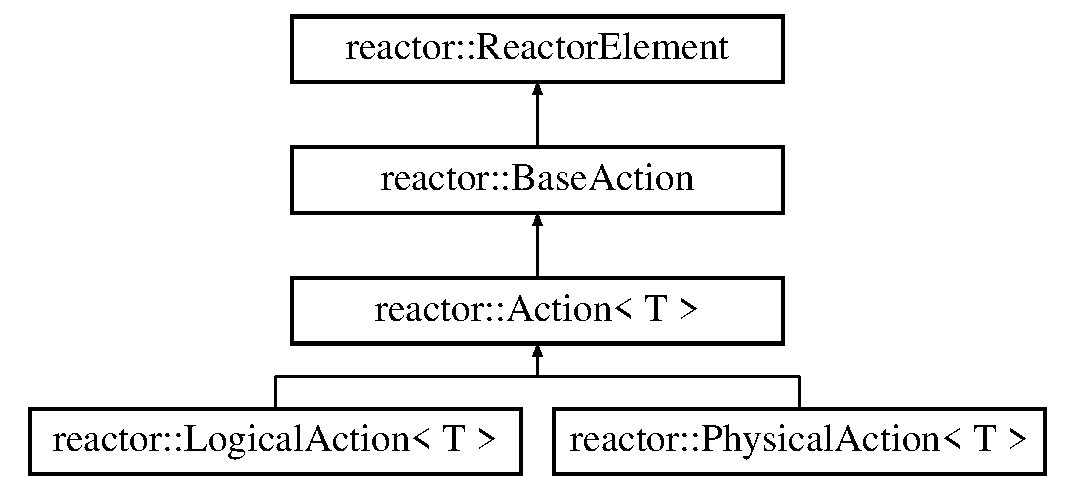
\includegraphics[height=4.000000cm]{classreactor_1_1Action}
\end{center}
\end{figure}
\subsection*{Public Member Functions}
\begin{DoxyCompactItemize}
\item 
void \hyperlink{classreactor_1_1Action_a60364e6742fb14dd515ff355abc5f3db}{startup} () override final
\item 
void \hyperlink{classreactor_1_1Action_a5e6698cc0893efca3a088f2158345b9c}{shutdown} () override final
\item 
{\footnotesize template$<$class Dur  = Duration$>$ }\\void \hyperlink{classreactor_1_1Action_a795f5b52075c020ec993d1149a720f62}{schedule} (const \hyperlink{classreactor_1_1ImmutableValuePtr}{Immutable\+Value\+Ptr}$<$ T $>$ \&\hyperlink{classreactor_1_1Action_a0002a99457bb578aa89854ad71db4fb2}{value\+\_\+ptr}, Dur delay=Dur\+::zero())
\item 
{\footnotesize template$<$class Dur  = Duration$>$ }\\void \hyperlink{classreactor_1_1Action_a863d3d618afb82404326c5076c9fd32a}{schedule} (\hyperlink{classreactor_1_1MutableValuePtr}{Mutable\+Value\+Ptr}$<$ T $>$ \&\&\hyperlink{classreactor_1_1Action_a0002a99457bb578aa89854ad71db4fb2}{value\+\_\+ptr}, Dur delay=Dur\+::zero())
\item 
{\footnotesize template$<$class Dur  = Duration$>$ }\\void \hyperlink{classreactor_1_1Action_a1dc2c0762950c330da3345f9192d62fa}{schedule} (const T \&value, Dur delay=Dur\+::zero())
\item 
{\footnotesize template$<$class Dur  = Duration$>$ }\\void \hyperlink{classreactor_1_1Action_ad8afb46b0b3bb753538cd37f7eae3be1}{schedule} (T \&\&value, Dur delay=Dur\+::zero())
\item 
const \hyperlink{classreactor_1_1ImmutableValuePtr}{Immutable\+Value\+Ptr}$<$ T $>$ \& \hyperlink{classreactor_1_1Action_a3b7937c4ce3f0a25562a08734ce8c2dc}{get} () const
\item 
bool \hyperlink{classreactor_1_1Action_a91d6979d528882d4aba1c892c130dbd1}{is\+\_\+present} () const
\end{DoxyCompactItemize}
\subsection*{Protected Member Functions}
\begin{DoxyCompactItemize}
\item 
\hyperlink{classreactor_1_1Action_ad0d36ea549eb0b04bd95d69fa8ac5d39}{Action} (const std\+::string \&\hyperlink{classreactor_1_1ReactorElement_a99579f61dbaf5d5d98aebfe26eb8bf77}{name}, \hyperlink{classreactor_1_1Reactor}{Reactor} $\ast$\hyperlink{classreactor_1_1ReactorElement_a25bf298de879a82eefc1ba426be05812}{container}, bool logical, \hyperlink{namespacereactor_aa8375b807a80703545664096c5b5b779}{Duration} \hyperlink{classreactor_1_1BaseAction_a98201db474f34cb9e38151a6960128f0}{min\+\_\+delay})
\end{DoxyCompactItemize}
\subsection*{Private Member Functions}
\begin{DoxyCompactItemize}
\item 
void \hyperlink{classreactor_1_1Action_a4ae275c1b030d5e8111469cc0ca5e09d}{cleanup} () override final
\end{DoxyCompactItemize}
\subsection*{Private Attributes}
\begin{DoxyCompactItemize}
\item 
\hyperlink{classreactor_1_1ImmutableValuePtr}{Immutable\+Value\+Ptr}$<$ T $>$ \hyperlink{classreactor_1_1Action_a0002a99457bb578aa89854ad71db4fb2}{value\+\_\+ptr} \{nullptr\}
\end{DoxyCompactItemize}
\subsection*{Additional Inherited Members}


\subsection{Constructor \& Destructor Documentation}
\mbox{\Hypertarget{classreactor_1_1Action_ad0d36ea549eb0b04bd95d69fa8ac5d39}\label{classreactor_1_1Action_ad0d36ea549eb0b04bd95d69fa8ac5d39}} 
\index{reactor\+::\+Action@{reactor\+::\+Action}!Action@{Action}}
\index{Action@{Action}!reactor\+::\+Action@{reactor\+::\+Action}}
\subsubsection{\texorpdfstring{Action()}{Action()}}
{\footnotesize\ttfamily template$<$class T $>$ \\
\hyperlink{classreactor_1_1Action}{reactor\+::\+Action}$<$ T $>$\+::\hyperlink{classreactor_1_1Action}{Action} (\begin{DoxyParamCaption}\item[{const std\+::string \&}]{name,  }\item[{\hyperlink{classreactor_1_1Reactor}{Reactor} $\ast$}]{container,  }\item[{bool}]{logical,  }\item[{\hyperlink{namespacereactor_aa8375b807a80703545664096c5b5b779}{Duration}}]{min\+\_\+delay }\end{DoxyParamCaption})\hspace{0.3cm}{\ttfamily [inline]}, {\ttfamily [protected]}}



\subsection{Member Function Documentation}
\mbox{\Hypertarget{classreactor_1_1Action_a4ae275c1b030d5e8111469cc0ca5e09d}\label{classreactor_1_1Action_a4ae275c1b030d5e8111469cc0ca5e09d}} 
\index{reactor\+::\+Action@{reactor\+::\+Action}!cleanup@{cleanup}}
\index{cleanup@{cleanup}!reactor\+::\+Action@{reactor\+::\+Action}}
\subsubsection{\texorpdfstring{cleanup()}{cleanup()}}
{\footnotesize\ttfamily template$<$class T $>$ \\
void \hyperlink{classreactor_1_1Action}{reactor\+::\+Action}$<$ T $>$\+::cleanup (\begin{DoxyParamCaption}{ }\end{DoxyParamCaption})\hspace{0.3cm}{\ttfamily [inline]}, {\ttfamily [final]}, {\ttfamily [override]}, {\ttfamily [private]}, {\ttfamily [virtual]}}



Implements \hyperlink{classreactor_1_1BaseAction_a7e4ad7157e653054c7afa22b78e46923}{reactor\+::\+Base\+Action}.

\mbox{\Hypertarget{classreactor_1_1Action_a3b7937c4ce3f0a25562a08734ce8c2dc}\label{classreactor_1_1Action_a3b7937c4ce3f0a25562a08734ce8c2dc}} 
\index{reactor\+::\+Action@{reactor\+::\+Action}!get@{get}}
\index{get@{get}!reactor\+::\+Action@{reactor\+::\+Action}}
\subsubsection{\texorpdfstring{get()}{get()}}
{\footnotesize\ttfamily template$<$class T $>$ \\
const \hyperlink{classreactor_1_1ImmutableValuePtr}{Immutable\+Value\+Ptr}$<$T$>$\& \hyperlink{classreactor_1_1Action}{reactor\+::\+Action}$<$ T $>$\+::get (\begin{DoxyParamCaption}{ }\end{DoxyParamCaption}) const\hspace{0.3cm}{\ttfamily [inline]}}

\mbox{\Hypertarget{classreactor_1_1Action_a91d6979d528882d4aba1c892c130dbd1}\label{classreactor_1_1Action_a91d6979d528882d4aba1c892c130dbd1}} 
\index{reactor\+::\+Action@{reactor\+::\+Action}!is\+\_\+present@{is\+\_\+present}}
\index{is\+\_\+present@{is\+\_\+present}!reactor\+::\+Action@{reactor\+::\+Action}}
\subsubsection{\texorpdfstring{is\+\_\+present()}{is\_present()}}
{\footnotesize\ttfamily template$<$class T $>$ \\
bool \hyperlink{classreactor_1_1Action}{reactor\+::\+Action}$<$ T $>$\+::is\+\_\+present (\begin{DoxyParamCaption}{ }\end{DoxyParamCaption}) const\hspace{0.3cm}{\ttfamily [inline]}}

\mbox{\Hypertarget{classreactor_1_1Action_a795f5b52075c020ec993d1149a720f62}\label{classreactor_1_1Action_a795f5b52075c020ec993d1149a720f62}} 
\index{reactor\+::\+Action@{reactor\+::\+Action}!schedule@{schedule}}
\index{schedule@{schedule}!reactor\+::\+Action@{reactor\+::\+Action}}
\subsubsection{\texorpdfstring{schedule()}{schedule()}\hspace{0.1cm}{\footnotesize\ttfamily [1/4]}}
{\footnotesize\ttfamily template$<$class T $>$ \\
template$<$class Dur $>$ \\
void \hyperlink{classreactor_1_1Action}{reactor\+::\+Action}$<$ T $>$\+::schedule (\begin{DoxyParamCaption}\item[{const \hyperlink{classreactor_1_1ImmutableValuePtr}{Immutable\+Value\+Ptr}$<$ T $>$ \&}]{value\+\_\+ptr,  }\item[{Dur}]{delay = {\ttfamily Dur\+:\+:zero()} }\end{DoxyParamCaption})}

\mbox{\Hypertarget{classreactor_1_1Action_a863d3d618afb82404326c5076c9fd32a}\label{classreactor_1_1Action_a863d3d618afb82404326c5076c9fd32a}} 
\index{reactor\+::\+Action@{reactor\+::\+Action}!schedule@{schedule}}
\index{schedule@{schedule}!reactor\+::\+Action@{reactor\+::\+Action}}
\subsubsection{\texorpdfstring{schedule()}{schedule()}\hspace{0.1cm}{\footnotesize\ttfamily [2/4]}}
{\footnotesize\ttfamily template$<$class T $>$ \\
template$<$class Dur  = Duration$>$ \\
void \hyperlink{classreactor_1_1Action}{reactor\+::\+Action}$<$ T $>$\+::schedule (\begin{DoxyParamCaption}\item[{\hyperlink{classreactor_1_1MutableValuePtr}{Mutable\+Value\+Ptr}$<$ T $>$ \&\&}]{value\+\_\+ptr,  }\item[{Dur}]{delay = {\ttfamily Dur\+:\+:zero()} }\end{DoxyParamCaption})\hspace{0.3cm}{\ttfamily [inline]}}

\mbox{\Hypertarget{classreactor_1_1Action_a1dc2c0762950c330da3345f9192d62fa}\label{classreactor_1_1Action_a1dc2c0762950c330da3345f9192d62fa}} 
\index{reactor\+::\+Action@{reactor\+::\+Action}!schedule@{schedule}}
\index{schedule@{schedule}!reactor\+::\+Action@{reactor\+::\+Action}}
\subsubsection{\texorpdfstring{schedule()}{schedule()}\hspace{0.1cm}{\footnotesize\ttfamily [3/4]}}
{\footnotesize\ttfamily template$<$class T $>$ \\
template$<$class Dur  = Duration$>$ \\
void \hyperlink{classreactor_1_1Action}{reactor\+::\+Action}$<$ T $>$\+::schedule (\begin{DoxyParamCaption}\item[{const T \&}]{value,  }\item[{Dur}]{delay = {\ttfamily Dur\+:\+:zero()} }\end{DoxyParamCaption})\hspace{0.3cm}{\ttfamily [inline]}}

\mbox{\Hypertarget{classreactor_1_1Action_ad8afb46b0b3bb753538cd37f7eae3be1}\label{classreactor_1_1Action_ad8afb46b0b3bb753538cd37f7eae3be1}} 
\index{reactor\+::\+Action@{reactor\+::\+Action}!schedule@{schedule}}
\index{schedule@{schedule}!reactor\+::\+Action@{reactor\+::\+Action}}
\subsubsection{\texorpdfstring{schedule()}{schedule()}\hspace{0.1cm}{\footnotesize\ttfamily [4/4]}}
{\footnotesize\ttfamily template$<$class T $>$ \\
template$<$class Dur  = Duration$>$ \\
void \hyperlink{classreactor_1_1Action}{reactor\+::\+Action}$<$ T $>$\+::schedule (\begin{DoxyParamCaption}\item[{T \&\&}]{value,  }\item[{Dur}]{delay = {\ttfamily Dur\+:\+:zero()} }\end{DoxyParamCaption})\hspace{0.3cm}{\ttfamily [inline]}}

\mbox{\Hypertarget{classreactor_1_1Action_a5e6698cc0893efca3a088f2158345b9c}\label{classreactor_1_1Action_a5e6698cc0893efca3a088f2158345b9c}} 
\index{reactor\+::\+Action@{reactor\+::\+Action}!shutdown@{shutdown}}
\index{shutdown@{shutdown}!reactor\+::\+Action@{reactor\+::\+Action}}
\subsubsection{\texorpdfstring{shutdown()}{shutdown()}}
{\footnotesize\ttfamily template$<$class T $>$ \\
void \hyperlink{classreactor_1_1Action}{reactor\+::\+Action}$<$ T $>$\+::shutdown (\begin{DoxyParamCaption}{ }\end{DoxyParamCaption})\hspace{0.3cm}{\ttfamily [inline]}, {\ttfamily [final]}, {\ttfamily [override]}, {\ttfamily [virtual]}}



Implements \hyperlink{classreactor_1_1ReactorElement_a8fce084bef582156979ebba56737e907}{reactor\+::\+Reactor\+Element}.

\mbox{\Hypertarget{classreactor_1_1Action_a60364e6742fb14dd515ff355abc5f3db}\label{classreactor_1_1Action_a60364e6742fb14dd515ff355abc5f3db}} 
\index{reactor\+::\+Action@{reactor\+::\+Action}!startup@{startup}}
\index{startup@{startup}!reactor\+::\+Action@{reactor\+::\+Action}}
\subsubsection{\texorpdfstring{startup()}{startup()}}
{\footnotesize\ttfamily template$<$class T $>$ \\
void \hyperlink{classreactor_1_1Action}{reactor\+::\+Action}$<$ T $>$\+::startup (\begin{DoxyParamCaption}{ }\end{DoxyParamCaption})\hspace{0.3cm}{\ttfamily [inline]}, {\ttfamily [final]}, {\ttfamily [override]}, {\ttfamily [virtual]}}



Implements \hyperlink{classreactor_1_1ReactorElement_a8cb574cb20ff963903ad905fb0a157e3}{reactor\+::\+Reactor\+Element}.



\subsection{Member Data Documentation}
\mbox{\Hypertarget{classreactor_1_1Action_a0002a99457bb578aa89854ad71db4fb2}\label{classreactor_1_1Action_a0002a99457bb578aa89854ad71db4fb2}} 
\index{reactor\+::\+Action@{reactor\+::\+Action}!value\+\_\+ptr@{value\+\_\+ptr}}
\index{value\+\_\+ptr@{value\+\_\+ptr}!reactor\+::\+Action@{reactor\+::\+Action}}
\subsubsection{\texorpdfstring{value\+\_\+ptr}{value\_ptr}}
{\footnotesize\ttfamily template$<$class T $>$ \\
\hyperlink{classreactor_1_1ImmutableValuePtr}{Immutable\+Value\+Ptr}$<$T$>$ \hyperlink{classreactor_1_1Action}{reactor\+::\+Action}$<$ T $>$\+::value\+\_\+ptr \{nullptr\}\hspace{0.3cm}{\ttfamily [private]}}



The documentation for this class was generated from the following files\+:\begin{DoxyCompactItemize}
\item 
/home/runner/work/reactor-\/cpp/reactor-\/cpp/include/reactor-\/cpp/\hyperlink{action_8hh}{action.\+hh}\item 
/home/runner/work/reactor-\/cpp/reactor-\/cpp/include/reactor-\/cpp/impl/\hyperlink{action__impl_8hh}{action\+\_\+impl.\+hh}\end{DoxyCompactItemize}

\hypertarget{classreactor_1_1Action_3_01void_01_4}{}\section{reactor\+:\+:Action$<$ void $>$ Class Template Reference}
\label{classreactor_1_1Action_3_01void_01_4}\index{reactor\+::\+Action$<$ void $>$@{reactor\+::\+Action$<$ void $>$}}


{\ttfamily \#include $<$action.\+hh$>$}

Inheritance diagram for reactor\+:\+:Action$<$ void $>$\+:\begin{figure}[H]
\begin{center}
\leavevmode
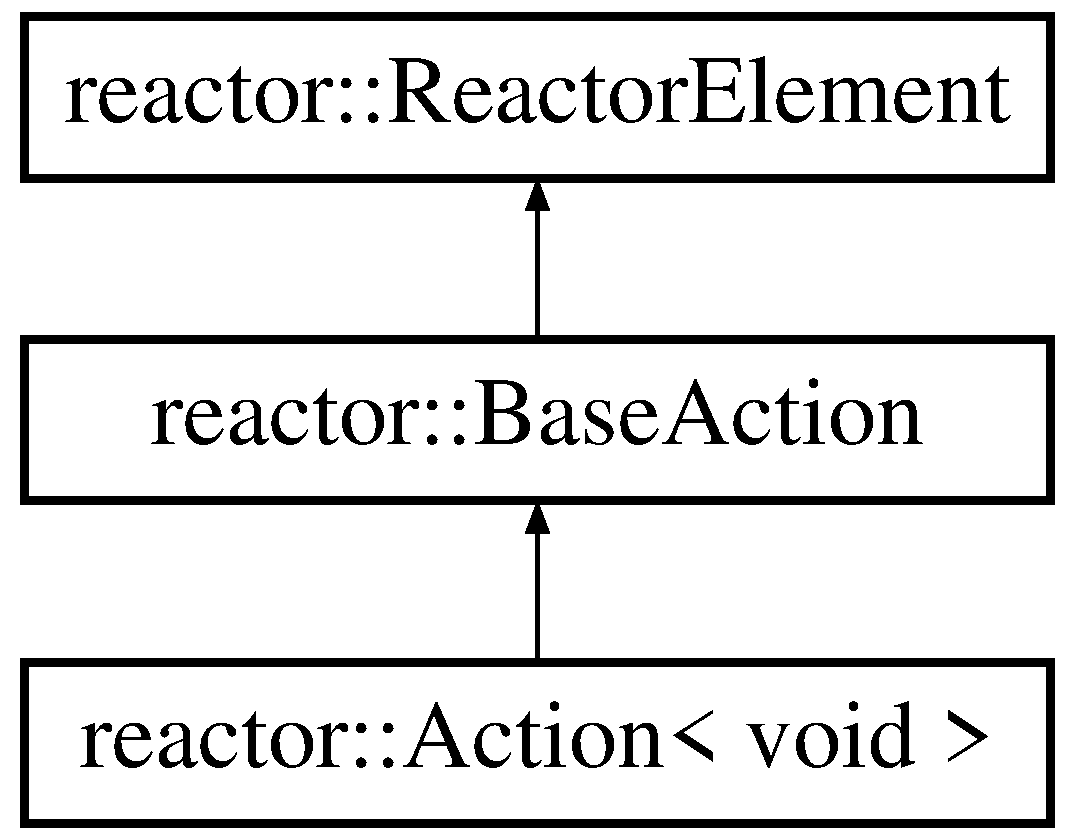
\includegraphics[height=3.000000cm]{classreactor_1_1Action_3_01void_01_4}
\end{center}
\end{figure}
\subsection*{Public Member Functions}
\begin{DoxyCompactItemize}
\item 
void \hyperlink{classreactor_1_1Action_3_01void_01_4_a6ba1aa14251401ebb7a4b13624d5ce92}{startup} () override final
\item 
void \hyperlink{classreactor_1_1Action_3_01void_01_4_a871645e568af7688eeacefbb65be4489}{shutdown} () override final
\item 
{\footnotesize template$<$class Dur  = Duration$>$ }\\void \hyperlink{classreactor_1_1Action_3_01void_01_4_aefb6d085020d1a60edbda6dce5dc033c}{schedule} (Dur delay=Dur\+::zero())
\item 
bool \hyperlink{classreactor_1_1Action_3_01void_01_4_a073662b60fddaebe09bba20082738120}{is\+\_\+present} () const
\end{DoxyCompactItemize}
\subsection*{Protected Member Functions}
\begin{DoxyCompactItemize}
\item 
\hyperlink{classreactor_1_1Action_3_01void_01_4_a74b23c4d882b046dc8e9aaad11e10eab}{Action} (const std\+::string \&\hyperlink{classreactor_1_1ReactorElement_a99579f61dbaf5d5d98aebfe26eb8bf77}{name}, \hyperlink{classreactor_1_1Reactor}{Reactor} $\ast$\hyperlink{classreactor_1_1ReactorElement_a25bf298de879a82eefc1ba426be05812}{container}, bool logical, \hyperlink{namespacereactor_aa8375b807a80703545664096c5b5b779}{Duration} \hyperlink{classreactor_1_1BaseAction_a98201db474f34cb9e38151a6960128f0}{min\+\_\+delay})
\end{DoxyCompactItemize}
\subsection*{Private Member Functions}
\begin{DoxyCompactItemize}
\item 
void \hyperlink{classreactor_1_1Action_3_01void_01_4_aa0306b1c370b15a324bac607e5f82f20}{cleanup} () override final
\end{DoxyCompactItemize}
\subsection*{Private Attributes}
\begin{DoxyCompactItemize}
\item 
bool \hyperlink{classreactor_1_1Action_3_01void_01_4_ad491b67ebfa70d65f04e6a0403a3cc51}{present} \{false\}
\end{DoxyCompactItemize}
\subsection*{Additional Inherited Members}


\subsection{Constructor \& Destructor Documentation}
\mbox{\Hypertarget{classreactor_1_1Action_3_01void_01_4_a74b23c4d882b046dc8e9aaad11e10eab}\label{classreactor_1_1Action_3_01void_01_4_a74b23c4d882b046dc8e9aaad11e10eab}} 
\index{reactor\+::\+Action$<$ void $>$@{reactor\+::\+Action$<$ void $>$}!Action@{Action}}
\index{Action@{Action}!reactor\+::\+Action$<$ void $>$@{reactor\+::\+Action$<$ void $>$}}
\subsubsection{\texorpdfstring{Action()}{Action()}}
{\footnotesize\ttfamily \hyperlink{classreactor_1_1Action}{reactor\+::\+Action}$<$ void $>$\+::\hyperlink{classreactor_1_1Action}{Action} (\begin{DoxyParamCaption}\item[{const std\+::string \&}]{name,  }\item[{\hyperlink{classreactor_1_1Reactor}{Reactor} $\ast$}]{container,  }\item[{bool}]{logical,  }\item[{\hyperlink{namespacereactor_aa8375b807a80703545664096c5b5b779}{Duration}}]{min\+\_\+delay }\end{DoxyParamCaption})\hspace{0.3cm}{\ttfamily [inline]}, {\ttfamily [protected]}}



\subsection{Member Function Documentation}
\mbox{\Hypertarget{classreactor_1_1Action_3_01void_01_4_aa0306b1c370b15a324bac607e5f82f20}\label{classreactor_1_1Action_3_01void_01_4_aa0306b1c370b15a324bac607e5f82f20}} 
\index{reactor\+::\+Action$<$ void $>$@{reactor\+::\+Action$<$ void $>$}!cleanup@{cleanup}}
\index{cleanup@{cleanup}!reactor\+::\+Action$<$ void $>$@{reactor\+::\+Action$<$ void $>$}}
\subsubsection{\texorpdfstring{cleanup()}{cleanup()}}
{\footnotesize\ttfamily void \hyperlink{classreactor_1_1Action}{reactor\+::\+Action}$<$ void $>$\+::cleanup (\begin{DoxyParamCaption}{ }\end{DoxyParamCaption})\hspace{0.3cm}{\ttfamily [inline]}, {\ttfamily [final]}, {\ttfamily [override]}, {\ttfamily [private]}, {\ttfamily [virtual]}}



Implements \hyperlink{classreactor_1_1BaseAction_a7e4ad7157e653054c7afa22b78e46923}{reactor\+::\+Base\+Action}.

\mbox{\Hypertarget{classreactor_1_1Action_3_01void_01_4_a073662b60fddaebe09bba20082738120}\label{classreactor_1_1Action_3_01void_01_4_a073662b60fddaebe09bba20082738120}} 
\index{reactor\+::\+Action$<$ void $>$@{reactor\+::\+Action$<$ void $>$}!is\+\_\+present@{is\+\_\+present}}
\index{is\+\_\+present@{is\+\_\+present}!reactor\+::\+Action$<$ void $>$@{reactor\+::\+Action$<$ void $>$}}
\subsubsection{\texorpdfstring{is\+\_\+present()}{is\_present()}}
{\footnotesize\ttfamily bool \hyperlink{classreactor_1_1Action}{reactor\+::\+Action}$<$ void $>$\+::is\+\_\+present (\begin{DoxyParamCaption}{ }\end{DoxyParamCaption}) const\hspace{0.3cm}{\ttfamily [inline]}}

\mbox{\Hypertarget{classreactor_1_1Action_3_01void_01_4_aefb6d085020d1a60edbda6dce5dc033c}\label{classreactor_1_1Action_3_01void_01_4_aefb6d085020d1a60edbda6dce5dc033c}} 
\index{reactor\+::\+Action$<$ void $>$@{reactor\+::\+Action$<$ void $>$}!schedule@{schedule}}
\index{schedule@{schedule}!reactor\+::\+Action$<$ void $>$@{reactor\+::\+Action$<$ void $>$}}
\subsubsection{\texorpdfstring{schedule()}{schedule()}}
{\footnotesize\ttfamily template$<$class Dur  = Duration$>$ \\
void \hyperlink{classreactor_1_1Action}{reactor\+::\+Action}$<$ void $>$\+::schedule (\begin{DoxyParamCaption}\item[{Dur}]{delay = {\ttfamily Dur\+:\+:zero()} }\end{DoxyParamCaption})}

\mbox{\Hypertarget{classreactor_1_1Action_3_01void_01_4_a871645e568af7688eeacefbb65be4489}\label{classreactor_1_1Action_3_01void_01_4_a871645e568af7688eeacefbb65be4489}} 
\index{reactor\+::\+Action$<$ void $>$@{reactor\+::\+Action$<$ void $>$}!shutdown@{shutdown}}
\index{shutdown@{shutdown}!reactor\+::\+Action$<$ void $>$@{reactor\+::\+Action$<$ void $>$}}
\subsubsection{\texorpdfstring{shutdown()}{shutdown()}}
{\footnotesize\ttfamily void \hyperlink{classreactor_1_1Action}{reactor\+::\+Action}$<$ void $>$\+::shutdown (\begin{DoxyParamCaption}{ }\end{DoxyParamCaption})\hspace{0.3cm}{\ttfamily [inline]}, {\ttfamily [final]}, {\ttfamily [override]}, {\ttfamily [virtual]}}



Implements \hyperlink{classreactor_1_1ReactorElement_a8fce084bef582156979ebba56737e907}{reactor\+::\+Reactor\+Element}.

\mbox{\Hypertarget{classreactor_1_1Action_3_01void_01_4_a6ba1aa14251401ebb7a4b13624d5ce92}\label{classreactor_1_1Action_3_01void_01_4_a6ba1aa14251401ebb7a4b13624d5ce92}} 
\index{reactor\+::\+Action$<$ void $>$@{reactor\+::\+Action$<$ void $>$}!startup@{startup}}
\index{startup@{startup}!reactor\+::\+Action$<$ void $>$@{reactor\+::\+Action$<$ void $>$}}
\subsubsection{\texorpdfstring{startup()}{startup()}}
{\footnotesize\ttfamily void \hyperlink{classreactor_1_1Action}{reactor\+::\+Action}$<$ void $>$\+::startup (\begin{DoxyParamCaption}{ }\end{DoxyParamCaption})\hspace{0.3cm}{\ttfamily [inline]}, {\ttfamily [final]}, {\ttfamily [override]}, {\ttfamily [virtual]}}



Implements \hyperlink{classreactor_1_1ReactorElement_a8cb574cb20ff963903ad905fb0a157e3}{reactor\+::\+Reactor\+Element}.



\subsection{Member Data Documentation}
\mbox{\Hypertarget{classreactor_1_1Action_3_01void_01_4_ad491b67ebfa70d65f04e6a0403a3cc51}\label{classreactor_1_1Action_3_01void_01_4_ad491b67ebfa70d65f04e6a0403a3cc51}} 
\index{reactor\+::\+Action$<$ void $>$@{reactor\+::\+Action$<$ void $>$}!present@{present}}
\index{present@{present}!reactor\+::\+Action$<$ void $>$@{reactor\+::\+Action$<$ void $>$}}
\subsubsection{\texorpdfstring{present}{present}}
{\footnotesize\ttfamily bool \hyperlink{classreactor_1_1Action}{reactor\+::\+Action}$<$ void $>$\+::present \{false\}\hspace{0.3cm}{\ttfamily [private]}}



The documentation for this class was generated from the following files\+:\begin{DoxyCompactItemize}
\item 
/home/runner/work/reactor-\/cpp/reactor-\/cpp/include/reactor-\/cpp/\hyperlink{action_8hh}{action.\+hh}\item 
/home/runner/work/reactor-\/cpp/reactor-\/cpp/include/reactor-\/cpp/impl/\hyperlink{action__impl_8hh}{action\+\_\+impl.\+hh}\end{DoxyCompactItemize}

\hypertarget{classreactor_1_1BaseAction}{}\section{reactor\+:\+:Base\+Action Class Reference}
\label{classreactor_1_1BaseAction}\index{reactor\+::\+Base\+Action@{reactor\+::\+Base\+Action}}


{\ttfamily \#include $<$action.\+hh$>$}

Inheritance diagram for reactor\+:\+:Base\+Action\+:\begin{figure}[H]
\begin{center}
\leavevmode
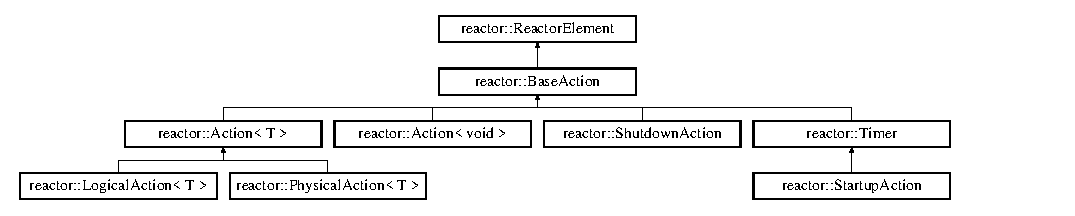
\includegraphics[height=2.461539cm]{classreactor_1_1BaseAction}
\end{center}
\end{figure}
\subsection*{Public Member Functions}
\begin{DoxyCompactItemize}
\item 
const auto \& \hyperlink{classreactor_1_1BaseAction_a330820b1a4bbe1b18d5b30773a690818}{triggers} () const
\item 
const auto \& \hyperlink{classreactor_1_1BaseAction_ac480015d4e2e2309fa7f9b2e2a7a59ab}{schedulers} () const
\item 
bool \hyperlink{classreactor_1_1BaseAction_abff8e7a40679e9f0d6d31eb795530279}{is\+\_\+logical} () const
\item 
bool \hyperlink{classreactor_1_1BaseAction_ae088220a837f00686793dd0a50629dc0}{is\+\_\+physical} () const
\end{DoxyCompactItemize}
\subsection*{Protected Member Functions}
\begin{DoxyCompactItemize}
\item 
void \hyperlink{classreactor_1_1BaseAction_a8ee41c1fd582f54518b6ca06b95a54ad}{register\+\_\+trigger} (\hyperlink{classreactor_1_1Reaction}{Reaction} $\ast$reaction)
\item 
void \hyperlink{classreactor_1_1BaseAction_a5cde20240a08d79c6c826d97f9a7f916}{register\+\_\+scheduler} (\hyperlink{classreactor_1_1Reaction}{Reaction} $\ast$reaction)
\item 
virtual void \hyperlink{classreactor_1_1BaseAction_a7e4ad7157e653054c7afa22b78e46923}{cleanup} ()=0
\item 
\hyperlink{classreactor_1_1BaseAction_a94dadf5eacb10e4e1d7bc99e53ac8599}{Base\+Action} (const std\+::string \&\hyperlink{classreactor_1_1ReactorElement_a99579f61dbaf5d5d98aebfe26eb8bf77}{name}, \hyperlink{classreactor_1_1Reactor}{Reactor} $\ast$\hyperlink{classreactor_1_1ReactorElement_a25bf298de879a82eefc1ba426be05812}{container}, bool logical, \hyperlink{namespacereactor_aa8375b807a80703545664096c5b5b779}{Duration} \hyperlink{classreactor_1_1BaseAction_a98201db474f34cb9e38151a6960128f0}{min\+\_\+delay})
\end{DoxyCompactItemize}
\subsection*{Protected Attributes}
\begin{DoxyCompactItemize}
\item 
const \hyperlink{namespacereactor_aa8375b807a80703545664096c5b5b779}{Duration} \hyperlink{classreactor_1_1BaseAction_a98201db474f34cb9e38151a6960128f0}{min\+\_\+delay}
\end{DoxyCompactItemize}
\subsection*{Private Attributes}
\begin{DoxyCompactItemize}
\item 
std\+::set$<$ \hyperlink{classreactor_1_1Reaction}{Reaction} $\ast$ $>$ \hyperlink{classreactor_1_1BaseAction_a90990090bd60f27c66b0cc7ddbc03b6e}{\+\_\+triggers}
\item 
std\+::set$<$ \hyperlink{classreactor_1_1Reaction}{Reaction} $\ast$ $>$ \hyperlink{classreactor_1_1BaseAction_a90459f877f25a143d9ad8c2fec8a402c}{\+\_\+schedulers}
\item 
const bool \hyperlink{classreactor_1_1BaseAction_adfef875bcf82270932d2a8648ea78796}{\+\_\+logical}
\end{DoxyCompactItemize}
\subsection*{Friends}
\begin{DoxyCompactItemize}
\item 
class \hyperlink{classreactor_1_1BaseAction_a5f86463029cca47f8aa15ff8cd5b9e51}{Reaction}
\item 
class \hyperlink{classreactor_1_1BaseAction_afb88c77ea5daaefa6c8fa6bc5b9aa5c1}{Scheduler}
\end{DoxyCompactItemize}
\subsection*{Additional Inherited Members}


\subsection{Constructor \& Destructor Documentation}
\mbox{\Hypertarget{classreactor_1_1BaseAction_a94dadf5eacb10e4e1d7bc99e53ac8599}\label{classreactor_1_1BaseAction_a94dadf5eacb10e4e1d7bc99e53ac8599}} 
\index{reactor\+::\+Base\+Action@{reactor\+::\+Base\+Action}!Base\+Action@{Base\+Action}}
\index{Base\+Action@{Base\+Action}!reactor\+::\+Base\+Action@{reactor\+::\+Base\+Action}}
\subsubsection{\texorpdfstring{Base\+Action()}{BaseAction()}}
{\footnotesize\ttfamily reactor\+::\+Base\+Action\+::\+Base\+Action (\begin{DoxyParamCaption}\item[{const std\+::string \&}]{name,  }\item[{\hyperlink{classreactor_1_1Reactor}{Reactor} $\ast$}]{container,  }\item[{bool}]{logical,  }\item[{\hyperlink{namespacereactor_aa8375b807a80703545664096c5b5b779}{Duration}}]{min\+\_\+delay }\end{DoxyParamCaption})\hspace{0.3cm}{\ttfamily [inline]}, {\ttfamily [protected]}}



\subsection{Member Function Documentation}
\mbox{\Hypertarget{classreactor_1_1BaseAction_a7e4ad7157e653054c7afa22b78e46923}\label{classreactor_1_1BaseAction_a7e4ad7157e653054c7afa22b78e46923}} 
\index{reactor\+::\+Base\+Action@{reactor\+::\+Base\+Action}!cleanup@{cleanup}}
\index{cleanup@{cleanup}!reactor\+::\+Base\+Action@{reactor\+::\+Base\+Action}}
\subsubsection{\texorpdfstring{cleanup()}{cleanup()}}
{\footnotesize\ttfamily virtual void reactor\+::\+Base\+Action\+::cleanup (\begin{DoxyParamCaption}{ }\end{DoxyParamCaption})\hspace{0.3cm}{\ttfamily [protected]}, {\ttfamily [pure virtual]}}



Implemented in \hyperlink{classreactor_1_1ShutdownAction_acbea47c7b7efb26cd10d6ac8c781901a}{reactor\+::\+Shutdown\+Action}, \hyperlink{classreactor_1_1Timer_ab01356b0c99de6a3bd9f46bfd0ce1c7b}{reactor\+::\+Timer}, \hyperlink{classreactor_1_1Action_3_01void_01_4_aa0306b1c370b15a324bac607e5f82f20}{reactor\+::\+Action$<$ void $>$}, and \hyperlink{classreactor_1_1Action_a4ae275c1b030d5e8111469cc0ca5e09d}{reactor\+::\+Action$<$ T $>$}.

\mbox{\Hypertarget{classreactor_1_1BaseAction_abff8e7a40679e9f0d6d31eb795530279}\label{classreactor_1_1BaseAction_abff8e7a40679e9f0d6d31eb795530279}} 
\index{reactor\+::\+Base\+Action@{reactor\+::\+Base\+Action}!is\+\_\+logical@{is\+\_\+logical}}
\index{is\+\_\+logical@{is\+\_\+logical}!reactor\+::\+Base\+Action@{reactor\+::\+Base\+Action}}
\subsubsection{\texorpdfstring{is\+\_\+logical()}{is\_logical()}}
{\footnotesize\ttfamily bool reactor\+::\+Base\+Action\+::is\+\_\+logical (\begin{DoxyParamCaption}{ }\end{DoxyParamCaption}) const\hspace{0.3cm}{\ttfamily [inline]}}

\mbox{\Hypertarget{classreactor_1_1BaseAction_ae088220a837f00686793dd0a50629dc0}\label{classreactor_1_1BaseAction_ae088220a837f00686793dd0a50629dc0}} 
\index{reactor\+::\+Base\+Action@{reactor\+::\+Base\+Action}!is\+\_\+physical@{is\+\_\+physical}}
\index{is\+\_\+physical@{is\+\_\+physical}!reactor\+::\+Base\+Action@{reactor\+::\+Base\+Action}}
\subsubsection{\texorpdfstring{is\+\_\+physical()}{is\_physical()}}
{\footnotesize\ttfamily bool reactor\+::\+Base\+Action\+::is\+\_\+physical (\begin{DoxyParamCaption}{ }\end{DoxyParamCaption}) const\hspace{0.3cm}{\ttfamily [inline]}}

\mbox{\Hypertarget{classreactor_1_1BaseAction_a5cde20240a08d79c6c826d97f9a7f916}\label{classreactor_1_1BaseAction_a5cde20240a08d79c6c826d97f9a7f916}} 
\index{reactor\+::\+Base\+Action@{reactor\+::\+Base\+Action}!register\+\_\+scheduler@{register\+\_\+scheduler}}
\index{register\+\_\+scheduler@{register\+\_\+scheduler}!reactor\+::\+Base\+Action@{reactor\+::\+Base\+Action}}
\subsubsection{\texorpdfstring{register\+\_\+scheduler()}{register\_scheduler()}}
{\footnotesize\ttfamily void reactor\+::\+Base\+Action\+::register\+\_\+scheduler (\begin{DoxyParamCaption}\item[{\hyperlink{classreactor_1_1Reaction}{Reaction} $\ast$}]{reaction }\end{DoxyParamCaption})\hspace{0.3cm}{\ttfamily [protected]}}

\mbox{\Hypertarget{classreactor_1_1BaseAction_a8ee41c1fd582f54518b6ca06b95a54ad}\label{classreactor_1_1BaseAction_a8ee41c1fd582f54518b6ca06b95a54ad}} 
\index{reactor\+::\+Base\+Action@{reactor\+::\+Base\+Action}!register\+\_\+trigger@{register\+\_\+trigger}}
\index{register\+\_\+trigger@{register\+\_\+trigger}!reactor\+::\+Base\+Action@{reactor\+::\+Base\+Action}}
\subsubsection{\texorpdfstring{register\+\_\+trigger()}{register\_trigger()}}
{\footnotesize\ttfamily void reactor\+::\+Base\+Action\+::register\+\_\+trigger (\begin{DoxyParamCaption}\item[{\hyperlink{classreactor_1_1Reaction}{Reaction} $\ast$}]{reaction }\end{DoxyParamCaption})\hspace{0.3cm}{\ttfamily [protected]}}

\mbox{\Hypertarget{classreactor_1_1BaseAction_ac480015d4e2e2309fa7f9b2e2a7a59ab}\label{classreactor_1_1BaseAction_ac480015d4e2e2309fa7f9b2e2a7a59ab}} 
\index{reactor\+::\+Base\+Action@{reactor\+::\+Base\+Action}!schedulers@{schedulers}}
\index{schedulers@{schedulers}!reactor\+::\+Base\+Action@{reactor\+::\+Base\+Action}}
\subsubsection{\texorpdfstring{schedulers()}{schedulers()}}
{\footnotesize\ttfamily const auto\& reactor\+::\+Base\+Action\+::schedulers (\begin{DoxyParamCaption}{ }\end{DoxyParamCaption}) const\hspace{0.3cm}{\ttfamily [inline]}}

\mbox{\Hypertarget{classreactor_1_1BaseAction_a330820b1a4bbe1b18d5b30773a690818}\label{classreactor_1_1BaseAction_a330820b1a4bbe1b18d5b30773a690818}} 
\index{reactor\+::\+Base\+Action@{reactor\+::\+Base\+Action}!triggers@{triggers}}
\index{triggers@{triggers}!reactor\+::\+Base\+Action@{reactor\+::\+Base\+Action}}
\subsubsection{\texorpdfstring{triggers()}{triggers()}}
{\footnotesize\ttfamily const auto\& reactor\+::\+Base\+Action\+::triggers (\begin{DoxyParamCaption}{ }\end{DoxyParamCaption}) const\hspace{0.3cm}{\ttfamily [inline]}}



\subsection{Friends And Related Function Documentation}
\mbox{\Hypertarget{classreactor_1_1BaseAction_a5f86463029cca47f8aa15ff8cd5b9e51}\label{classreactor_1_1BaseAction_a5f86463029cca47f8aa15ff8cd5b9e51}} 
\index{reactor\+::\+Base\+Action@{reactor\+::\+Base\+Action}!Reaction@{Reaction}}
\index{Reaction@{Reaction}!reactor\+::\+Base\+Action@{reactor\+::\+Base\+Action}}
\subsubsection{\texorpdfstring{Reaction}{Reaction}}
{\footnotesize\ttfamily friend class \hyperlink{classreactor_1_1Reaction}{Reaction}\hspace{0.3cm}{\ttfamily [friend]}}

\mbox{\Hypertarget{classreactor_1_1BaseAction_afb88c77ea5daaefa6c8fa6bc5b9aa5c1}\label{classreactor_1_1BaseAction_afb88c77ea5daaefa6c8fa6bc5b9aa5c1}} 
\index{reactor\+::\+Base\+Action@{reactor\+::\+Base\+Action}!Scheduler@{Scheduler}}
\index{Scheduler@{Scheduler}!reactor\+::\+Base\+Action@{reactor\+::\+Base\+Action}}
\subsubsection{\texorpdfstring{Scheduler}{Scheduler}}
{\footnotesize\ttfamily friend class \hyperlink{classreactor_1_1Scheduler}{Scheduler}\hspace{0.3cm}{\ttfamily [friend]}}



\subsection{Member Data Documentation}
\mbox{\Hypertarget{classreactor_1_1BaseAction_adfef875bcf82270932d2a8648ea78796}\label{classreactor_1_1BaseAction_adfef875bcf82270932d2a8648ea78796}} 
\index{reactor\+::\+Base\+Action@{reactor\+::\+Base\+Action}!\+\_\+logical@{\+\_\+logical}}
\index{\+\_\+logical@{\+\_\+logical}!reactor\+::\+Base\+Action@{reactor\+::\+Base\+Action}}
\subsubsection{\texorpdfstring{\+\_\+logical}{\_logical}}
{\footnotesize\ttfamily const bool reactor\+::\+Base\+Action\+::\+\_\+logical\hspace{0.3cm}{\ttfamily [private]}}

\mbox{\Hypertarget{classreactor_1_1BaseAction_a90459f877f25a143d9ad8c2fec8a402c}\label{classreactor_1_1BaseAction_a90459f877f25a143d9ad8c2fec8a402c}} 
\index{reactor\+::\+Base\+Action@{reactor\+::\+Base\+Action}!\+\_\+schedulers@{\+\_\+schedulers}}
\index{\+\_\+schedulers@{\+\_\+schedulers}!reactor\+::\+Base\+Action@{reactor\+::\+Base\+Action}}
\subsubsection{\texorpdfstring{\+\_\+schedulers}{\_schedulers}}
{\footnotesize\ttfamily std\+::set$<$\hyperlink{classreactor_1_1Reaction}{Reaction}$\ast$$>$ reactor\+::\+Base\+Action\+::\+\_\+schedulers\hspace{0.3cm}{\ttfamily [private]}}

\mbox{\Hypertarget{classreactor_1_1BaseAction_a90990090bd60f27c66b0cc7ddbc03b6e}\label{classreactor_1_1BaseAction_a90990090bd60f27c66b0cc7ddbc03b6e}} 
\index{reactor\+::\+Base\+Action@{reactor\+::\+Base\+Action}!\+\_\+triggers@{\+\_\+triggers}}
\index{\+\_\+triggers@{\+\_\+triggers}!reactor\+::\+Base\+Action@{reactor\+::\+Base\+Action}}
\subsubsection{\texorpdfstring{\+\_\+triggers}{\_triggers}}
{\footnotesize\ttfamily std\+::set$<$\hyperlink{classreactor_1_1Reaction}{Reaction}$\ast$$>$ reactor\+::\+Base\+Action\+::\+\_\+triggers\hspace{0.3cm}{\ttfamily [private]}}

\mbox{\Hypertarget{classreactor_1_1BaseAction_a98201db474f34cb9e38151a6960128f0}\label{classreactor_1_1BaseAction_a98201db474f34cb9e38151a6960128f0}} 
\index{reactor\+::\+Base\+Action@{reactor\+::\+Base\+Action}!min\+\_\+delay@{min\+\_\+delay}}
\index{min\+\_\+delay@{min\+\_\+delay}!reactor\+::\+Base\+Action@{reactor\+::\+Base\+Action}}
\subsubsection{\texorpdfstring{min\+\_\+delay}{min\_delay}}
{\footnotesize\ttfamily const \hyperlink{namespacereactor_aa8375b807a80703545664096c5b5b779}{Duration} reactor\+::\+Base\+Action\+::min\+\_\+delay\hspace{0.3cm}{\ttfamily [protected]}}



The documentation for this class was generated from the following files\+:\begin{DoxyCompactItemize}
\item 
/home/runner/work/reactor-\/cpp/reactor-\/cpp/include/reactor-\/cpp/\hyperlink{action_8hh}{action.\+hh}\item 
/home/runner/work/reactor-\/cpp/reactor-\/cpp/lib/\hyperlink{action_8cc}{action.\+cc}\end{DoxyCompactItemize}

\hypertarget{classreactor_1_1log_1_1BaseLogger}{}\section{reactor\+:\+:log\+:\+:Base\+Logger$<$ enabled $>$ Class Template Reference}
\label{classreactor_1_1log_1_1BaseLogger}\index{reactor\+::log\+::\+Base\+Logger$<$ enabled $>$@{reactor\+::log\+::\+Base\+Logger$<$ enabled $>$}}


{\ttfamily \#include $<$logging.\+hh$>$}



The documentation for this class was generated from the following file\+:\begin{DoxyCompactItemize}
\item 
/home/runner/work/reactor-\/cpp/reactor-\/cpp/include/reactor-\/cpp/\hyperlink{logging_8hh}{logging.\+hh}\end{DoxyCompactItemize}

\hypertarget{classreactor_1_1log_1_1BaseLogger_3_01false_01_4}{}\section{reactor\+:\+:log\+:\+:Base\+Logger$<$ false $>$ Class Template Reference}
\label{classreactor_1_1log_1_1BaseLogger_3_01false_01_4}\index{reactor\+::log\+::\+Base\+Logger$<$ false $>$@{reactor\+::log\+::\+Base\+Logger$<$ false $>$}}


{\ttfamily \#include $<$logging.\+hh$>$}

\subsection*{Public Member Functions}
\begin{DoxyCompactItemize}
\item 
\hyperlink{classreactor_1_1log_1_1BaseLogger_3_01false_01_4_a573e2132fc169e4187df6965c5702d30}{Base\+Logger} (const std\+::string \&)
\item 
{\footnotesize template$<$class T $>$ }\\const \hyperlink{classreactor_1_1log_1_1BaseLogger}{Base\+Logger} \& \hyperlink{classreactor_1_1log_1_1BaseLogger_3_01false_01_4_a871b558bb1f64ed564deb55a1286d56c}{operator$<$$<$} (const T \&) const
\item 
\hyperlink{classreactor_1_1log_1_1BaseLogger_3_01false_01_4_a3b4c1ce4ef1f745c151fbbafceba3013}{$\sim$\+Base\+Logger} ()
\end{DoxyCompactItemize}


\subsection{Constructor \& Destructor Documentation}
\mbox{\Hypertarget{classreactor_1_1log_1_1BaseLogger_3_01false_01_4_a573e2132fc169e4187df6965c5702d30}\label{classreactor_1_1log_1_1BaseLogger_3_01false_01_4_a573e2132fc169e4187df6965c5702d30}} 
\index{reactor\+::log\+::\+Base\+Logger$<$ false $>$@{reactor\+::log\+::\+Base\+Logger$<$ false $>$}!Base\+Logger@{Base\+Logger}}
\index{Base\+Logger@{Base\+Logger}!reactor\+::log\+::\+Base\+Logger$<$ false $>$@{reactor\+::log\+::\+Base\+Logger$<$ false $>$}}
\subsubsection{\texorpdfstring{Base\+Logger()}{BaseLogger()}}
{\footnotesize\ttfamily \hyperlink{classreactor_1_1log_1_1BaseLogger}{reactor\+::log\+::\+Base\+Logger}$<$ false $>$\+::\hyperlink{classreactor_1_1log_1_1BaseLogger}{Base\+Logger} (\begin{DoxyParamCaption}\item[{const std\+::string \&}]{ }\end{DoxyParamCaption})\hspace{0.3cm}{\ttfamily [inline]}}

\mbox{\Hypertarget{classreactor_1_1log_1_1BaseLogger_3_01false_01_4_a3b4c1ce4ef1f745c151fbbafceba3013}\label{classreactor_1_1log_1_1BaseLogger_3_01false_01_4_a3b4c1ce4ef1f745c151fbbafceba3013}} 
\index{reactor\+::log\+::\+Base\+Logger$<$ false $>$@{reactor\+::log\+::\+Base\+Logger$<$ false $>$}!````~Base\+Logger@{$\sim$\+Base\+Logger}}
\index{````~Base\+Logger@{$\sim$\+Base\+Logger}!reactor\+::log\+::\+Base\+Logger$<$ false $>$@{reactor\+::log\+::\+Base\+Logger$<$ false $>$}}
\subsubsection{\texorpdfstring{$\sim$\+Base\+Logger()}{~BaseLogger()}}
{\footnotesize\ttfamily \hyperlink{classreactor_1_1log_1_1BaseLogger}{reactor\+::log\+::\+Base\+Logger}$<$ false $>$\+::$\sim$\hyperlink{classreactor_1_1log_1_1BaseLogger}{Base\+Logger} (\begin{DoxyParamCaption}{ }\end{DoxyParamCaption})\hspace{0.3cm}{\ttfamily [inline]}}



\subsection{Member Function Documentation}
\mbox{\Hypertarget{classreactor_1_1log_1_1BaseLogger_3_01false_01_4_a871b558bb1f64ed564deb55a1286d56c}\label{classreactor_1_1log_1_1BaseLogger_3_01false_01_4_a871b558bb1f64ed564deb55a1286d56c}} 
\index{reactor\+::log\+::\+Base\+Logger$<$ false $>$@{reactor\+::log\+::\+Base\+Logger$<$ false $>$}!operator$<$$<$@{operator$<$$<$}}
\index{operator$<$$<$@{operator$<$$<$}!reactor\+::log\+::\+Base\+Logger$<$ false $>$@{reactor\+::log\+::\+Base\+Logger$<$ false $>$}}
\subsubsection{\texorpdfstring{operator$<$$<$()}{operator<<()}}
{\footnotesize\ttfamily template$<$class T $>$ \\
const \hyperlink{classreactor_1_1log_1_1BaseLogger}{Base\+Logger}\& \hyperlink{classreactor_1_1log_1_1BaseLogger}{reactor\+::log\+::\+Base\+Logger}$<$ false $>$\+::operator$<$$<$ (\begin{DoxyParamCaption}\item[{const T \&}]{ }\end{DoxyParamCaption}) const\hspace{0.3cm}{\ttfamily [inline]}}



The documentation for this class was generated from the following file\+:\begin{DoxyCompactItemize}
\item 
/home/runner/work/reactor-\/cpp/reactor-\/cpp/include/reactor-\/cpp/\hyperlink{logging_8hh}{logging.\+hh}\end{DoxyCompactItemize}

\hypertarget{classreactor_1_1log_1_1BaseLogger_3_01true_01_4}{}\section{reactor\+:\+:log\+:\+:Base\+Logger$<$ true $>$ Class Template Reference}
\label{classreactor_1_1log_1_1BaseLogger_3_01true_01_4}\index{reactor\+::log\+::\+Base\+Logger$<$ true $>$@{reactor\+::log\+::\+Base\+Logger$<$ true $>$}}


{\ttfamily \#include $<$logging.\+hh$>$}

\subsection*{Public Member Functions}
\begin{DoxyCompactItemize}
\item 
\hyperlink{classreactor_1_1log_1_1BaseLogger_3_01true_01_4_af11fb9ca0a141bdb7d5c14f3931735f9}{Base\+Logger} (const std\+::string \&\hyperlink{classreactor_1_1log_1_1BaseLogger_3_01true_01_4_ac12deb548273b6b993a0153ace1e6cdc}{log\+\_\+prefix})
\item 
{\footnotesize template$<$class T $>$ }\\\hyperlink{classreactor_1_1log_1_1BaseLogger}{Base\+Logger} \& \hyperlink{classreactor_1_1log_1_1BaseLogger_3_01true_01_4_a0ed6724c737335c58ddb1d3352ba58b9}{operator$<$$<$} (const T \&msg)
\item 
\hyperlink{classreactor_1_1log_1_1BaseLogger_3_01true_01_4_a1c4cf99b3f0d8c2f1c7761e7e5daa02e}{$\sim$\+Base\+Logger} ()
\end{DoxyCompactItemize}
\subsection*{Private Types}
\begin{DoxyCompactItemize}
\item 
using \hyperlink{classreactor_1_1log_1_1BaseLogger_3_01true_01_4_a145f94a8210bc4c9bbf54c3af61bd8ce}{Lock} = std\+::unique\+\_\+lock$<$ std\+::mutex $>$
\end{DoxyCompactItemize}
\subsection*{Private Attributes}
\begin{DoxyCompactItemize}
\item 
const std\+::string \hyperlink{classreactor_1_1log_1_1BaseLogger_3_01true_01_4_ac12deb548273b6b993a0153ace1e6cdc}{log\+\_\+prefix}
\item 
\hyperlink{classreactor_1_1log_1_1BaseLogger_3_01true_01_4_a145f94a8210bc4c9bbf54c3af61bd8ce}{Lock} \hyperlink{classreactor_1_1log_1_1BaseLogger_3_01true_01_4_a7a9e073069a113bdabc80230f9cefb12}{lock}
\end{DoxyCompactItemize}
\subsection*{Static Private Attributes}
\begin{DoxyCompactItemize}
\item 
static std\+::mutex \hyperlink{classreactor_1_1log_1_1BaseLogger_3_01true_01_4_a8991911bde1823d50152926e3241c186}{mutex}
\end{DoxyCompactItemize}


\subsection{Member Typedef Documentation}
\mbox{\Hypertarget{classreactor_1_1log_1_1BaseLogger_3_01true_01_4_a145f94a8210bc4c9bbf54c3af61bd8ce}\label{classreactor_1_1log_1_1BaseLogger_3_01true_01_4_a145f94a8210bc4c9bbf54c3af61bd8ce}} 
\index{reactor\+::log\+::\+Base\+Logger$<$ true $>$@{reactor\+::log\+::\+Base\+Logger$<$ true $>$}!Lock@{Lock}}
\index{Lock@{Lock}!reactor\+::log\+::\+Base\+Logger$<$ true $>$@{reactor\+::log\+::\+Base\+Logger$<$ true $>$}}
\subsubsection{\texorpdfstring{Lock}{Lock}}
{\footnotesize\ttfamily using \hyperlink{classreactor_1_1log_1_1BaseLogger}{reactor\+::log\+::\+Base\+Logger}$<$ true $>$\+::\hyperlink{classreactor_1_1log_1_1BaseLogger_3_01true_01_4_a145f94a8210bc4c9bbf54c3af61bd8ce}{Lock} =  std\+::unique\+\_\+lock$<$std\+::mutex$>$\hspace{0.3cm}{\ttfamily [private]}}



\subsection{Constructor \& Destructor Documentation}
\mbox{\Hypertarget{classreactor_1_1log_1_1BaseLogger_3_01true_01_4_af11fb9ca0a141bdb7d5c14f3931735f9}\label{classreactor_1_1log_1_1BaseLogger_3_01true_01_4_af11fb9ca0a141bdb7d5c14f3931735f9}} 
\index{reactor\+::log\+::\+Base\+Logger$<$ true $>$@{reactor\+::log\+::\+Base\+Logger$<$ true $>$}!Base\+Logger@{Base\+Logger}}
\index{Base\+Logger@{Base\+Logger}!reactor\+::log\+::\+Base\+Logger$<$ true $>$@{reactor\+::log\+::\+Base\+Logger$<$ true $>$}}
\subsubsection{\texorpdfstring{Base\+Logger()}{BaseLogger()}}
{\footnotesize\ttfamily \hyperlink{classreactor_1_1log_1_1BaseLogger}{reactor\+::log\+::\+Base\+Logger}$<$ true $>$\+::\hyperlink{classreactor_1_1log_1_1BaseLogger}{Base\+Logger} (\begin{DoxyParamCaption}\item[{const std\+::string \&}]{log\+\_\+prefix }\end{DoxyParamCaption})\hspace{0.3cm}{\ttfamily [inline]}}

\mbox{\Hypertarget{classreactor_1_1log_1_1BaseLogger_3_01true_01_4_a1c4cf99b3f0d8c2f1c7761e7e5daa02e}\label{classreactor_1_1log_1_1BaseLogger_3_01true_01_4_a1c4cf99b3f0d8c2f1c7761e7e5daa02e}} 
\index{reactor\+::log\+::\+Base\+Logger$<$ true $>$@{reactor\+::log\+::\+Base\+Logger$<$ true $>$}!````~Base\+Logger@{$\sim$\+Base\+Logger}}
\index{````~Base\+Logger@{$\sim$\+Base\+Logger}!reactor\+::log\+::\+Base\+Logger$<$ true $>$@{reactor\+::log\+::\+Base\+Logger$<$ true $>$}}
\subsubsection{\texorpdfstring{$\sim$\+Base\+Logger()}{~BaseLogger()}}
{\footnotesize\ttfamily \hyperlink{classreactor_1_1log_1_1BaseLogger}{reactor\+::log\+::\+Base\+Logger}$<$ true $>$\+::$\sim$\hyperlink{classreactor_1_1log_1_1BaseLogger}{Base\+Logger} (\begin{DoxyParamCaption}{ }\end{DoxyParamCaption})\hspace{0.3cm}{\ttfamily [inline]}}



\subsection{Member Function Documentation}
\mbox{\Hypertarget{classreactor_1_1log_1_1BaseLogger_3_01true_01_4_a0ed6724c737335c58ddb1d3352ba58b9}\label{classreactor_1_1log_1_1BaseLogger_3_01true_01_4_a0ed6724c737335c58ddb1d3352ba58b9}} 
\index{reactor\+::log\+::\+Base\+Logger$<$ true $>$@{reactor\+::log\+::\+Base\+Logger$<$ true $>$}!operator$<$$<$@{operator$<$$<$}}
\index{operator$<$$<$@{operator$<$$<$}!reactor\+::log\+::\+Base\+Logger$<$ true $>$@{reactor\+::log\+::\+Base\+Logger$<$ true $>$}}
\subsubsection{\texorpdfstring{operator$<$$<$()}{operator<<()}}
{\footnotesize\ttfamily template$<$class T $>$ \\
\hyperlink{classreactor_1_1log_1_1BaseLogger}{Base\+Logger}\& \hyperlink{classreactor_1_1log_1_1BaseLogger}{reactor\+::log\+::\+Base\+Logger}$<$ true $>$\+::operator$<$$<$ (\begin{DoxyParamCaption}\item[{const T \&}]{msg }\end{DoxyParamCaption})\hspace{0.3cm}{\ttfamily [inline]}}



\subsection{Member Data Documentation}
\mbox{\Hypertarget{classreactor_1_1log_1_1BaseLogger_3_01true_01_4_a7a9e073069a113bdabc80230f9cefb12}\label{classreactor_1_1log_1_1BaseLogger_3_01true_01_4_a7a9e073069a113bdabc80230f9cefb12}} 
\index{reactor\+::log\+::\+Base\+Logger$<$ true $>$@{reactor\+::log\+::\+Base\+Logger$<$ true $>$}!lock@{lock}}
\index{lock@{lock}!reactor\+::log\+::\+Base\+Logger$<$ true $>$@{reactor\+::log\+::\+Base\+Logger$<$ true $>$}}
\subsubsection{\texorpdfstring{lock}{lock}}
{\footnotesize\ttfamily \hyperlink{classreactor_1_1log_1_1BaseLogger_3_01true_01_4_a145f94a8210bc4c9bbf54c3af61bd8ce}{Lock} \hyperlink{classreactor_1_1log_1_1BaseLogger}{reactor\+::log\+::\+Base\+Logger}$<$ true $>$\+::lock\hspace{0.3cm}{\ttfamily [private]}}

\mbox{\Hypertarget{classreactor_1_1log_1_1BaseLogger_3_01true_01_4_ac12deb548273b6b993a0153ace1e6cdc}\label{classreactor_1_1log_1_1BaseLogger_3_01true_01_4_ac12deb548273b6b993a0153ace1e6cdc}} 
\index{reactor\+::log\+::\+Base\+Logger$<$ true $>$@{reactor\+::log\+::\+Base\+Logger$<$ true $>$}!log\+\_\+prefix@{log\+\_\+prefix}}
\index{log\+\_\+prefix@{log\+\_\+prefix}!reactor\+::log\+::\+Base\+Logger$<$ true $>$@{reactor\+::log\+::\+Base\+Logger$<$ true $>$}}
\subsubsection{\texorpdfstring{log\+\_\+prefix}{log\_prefix}}
{\footnotesize\ttfamily const std\+::string \hyperlink{classreactor_1_1log_1_1BaseLogger}{reactor\+::log\+::\+Base\+Logger}$<$ true $>$\+::log\+\_\+prefix\hspace{0.3cm}{\ttfamily [private]}}

\mbox{\Hypertarget{classreactor_1_1log_1_1BaseLogger_3_01true_01_4_a8991911bde1823d50152926e3241c186}\label{classreactor_1_1log_1_1BaseLogger_3_01true_01_4_a8991911bde1823d50152926e3241c186}} 
\index{reactor\+::log\+::\+Base\+Logger$<$ true $>$@{reactor\+::log\+::\+Base\+Logger$<$ true $>$}!mutex@{mutex}}
\index{mutex@{mutex}!reactor\+::log\+::\+Base\+Logger$<$ true $>$@{reactor\+::log\+::\+Base\+Logger$<$ true $>$}}
\subsubsection{\texorpdfstring{mutex}{mutex}}
{\footnotesize\ttfamily std\+::mutex \hyperlink{classreactor_1_1log_1_1BaseLogger}{reactor\+::log\+::\+Base\+Logger}$<$ true $>$\+::mutex\hspace{0.3cm}{\ttfamily [static]}, {\ttfamily [private]}}



The documentation for this class was generated from the following files\+:\begin{DoxyCompactItemize}
\item 
/home/runner/work/reactor-\/cpp/reactor-\/cpp/include/reactor-\/cpp/\hyperlink{logging_8hh}{logging.\+hh}\item 
/home/runner/work/reactor-\/cpp/reactor-\/cpp/lib/\hyperlink{logging_8cc}{logging.\+cc}\end{DoxyCompactItemize}

\hypertarget{classreactor_1_1BasePort}{}\section{reactor\+:\+:Base\+Port Class Reference}
\label{classreactor_1_1BasePort}\index{reactor\+::\+Base\+Port@{reactor\+::\+Base\+Port}}


{\ttfamily \#include $<$port.\+hh$>$}

Inheritance diagram for reactor\+:\+:Base\+Port\+:\begin{figure}[H]
\begin{center}
\leavevmode
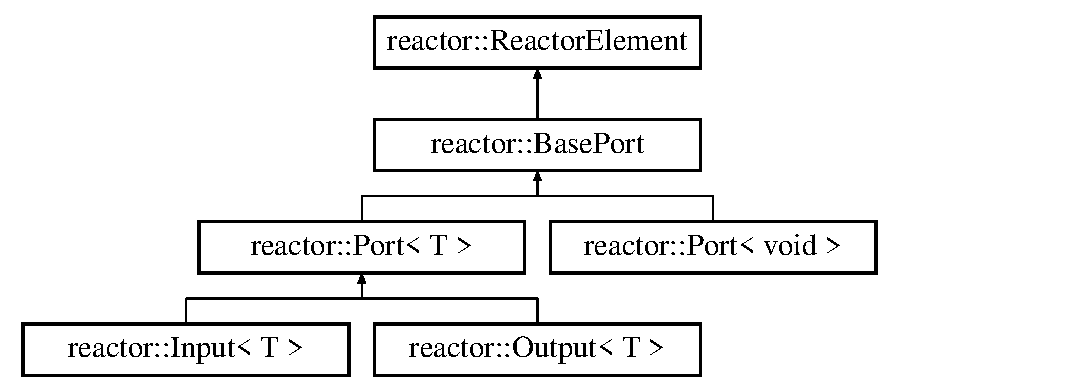
\includegraphics[height=4.000000cm]{classreactor_1_1BasePort}
\end{center}
\end{figure}
\subsection*{Public Member Functions}
\begin{DoxyCompactItemize}
\item 
bool \hyperlink{classreactor_1_1BasePort_ad488760a5ed50b9bbf137d4e52c053f7}{is\+\_\+input} () const
\item 
bool \hyperlink{classreactor_1_1BasePort_ad5ebded21426bfcf02359b1ab3fdf7d8}{is\+\_\+output} () const
\item 
bool \hyperlink{classreactor_1_1BasePort_a8d8a93a2d15683d29ec7a4ec483db01a}{has\+\_\+inward\+\_\+binding} () const
\item 
bool \hyperlink{classreactor_1_1BasePort_a397f8bbc24835a01bfad591abb85bcb4}{has\+\_\+outward\+\_\+bindings} () const
\item 
bool \hyperlink{classreactor_1_1BasePort_a687c0460c4823d90d150c6a363e256a9}{has\+\_\+dependencies} () const
\item 
bool \hyperlink{classreactor_1_1BasePort_a0c046ef79ccf68f8a68f788df774aed3}{has\+\_\+antidependencies} () const
\item 
\hyperlink{classreactor_1_1BasePort}{Base\+Port} $\ast$ \hyperlink{classreactor_1_1BasePort_af4a42f14f878509c00bb16d0c5b2c201}{inward\+\_\+binding} () const
\item 
const auto \& \hyperlink{classreactor_1_1BasePort_aaf404379c3908577b7fc7e394d5c972c}{outward\+\_\+bindings} () const
\item 
const auto \& \hyperlink{classreactor_1_1BasePort_a71208c7024e39242b1012091daf7b7ed}{triggers} () const
\item 
const auto \& \hyperlink{classreactor_1_1BasePort_aab124dee21981b289b55c2e2c8e3922d}{dependencies} () const
\item 
const auto \& \hyperlink{classreactor_1_1BasePort_a9158ab37ab600ea2b8a39749ca9404c4}{antidependencies} () const
\end{DoxyCompactItemize}
\subsection*{Protected Member Functions}
\begin{DoxyCompactItemize}
\item 
\hyperlink{classreactor_1_1BasePort_abf23bbb8fdd982044fca7d253ca1d851}{Base\+Port} (const std\+::string \&\hyperlink{classreactor_1_1ReactorElement_a99579f61dbaf5d5d98aebfe26eb8bf77}{name}, \hyperlink{namespacereactor_a08c8e2d85e5bc706b1af8a87e40eec6d}{Port\+Type} \hyperlink{classreactor_1_1BasePort_a9af5e0d55ee1a425b2c5975ab1ca871e}{type}, \hyperlink{classreactor_1_1Reactor}{Reactor} $\ast$\hyperlink{classreactor_1_1ReactorElement_a25bf298de879a82eefc1ba426be05812}{container})
\item 
void \hyperlink{classreactor_1_1BasePort_a58886ca9004547c85b06e7803d0530b1}{base\+\_\+bind\+\_\+to} (\hyperlink{classreactor_1_1BasePort}{Base\+Port} $\ast$port)
\item 
void \hyperlink{classreactor_1_1BasePort_a781809b23cbb205087867bddbd077e17}{register\+\_\+dependency} (\hyperlink{classreactor_1_1Reaction}{Reaction} $\ast$reaction, bool is\+\_\+trigger)
\item 
void \hyperlink{classreactor_1_1BasePort_a1a9831f2c5dfb36c1c0987ab7dcdd608}{register\+\_\+antidependency} (\hyperlink{classreactor_1_1Reaction}{Reaction} $\ast$reaction)
\item 
virtual void \hyperlink{classreactor_1_1BasePort_afe81e6747077349da4c420a873783579}{cleanup} ()=0
\end{DoxyCompactItemize}
\subsection*{Private Attributes}
\begin{DoxyCompactItemize}
\item 
\hyperlink{classreactor_1_1BasePort}{Base\+Port} $\ast$ \hyperlink{classreactor_1_1BasePort_a2a457c372d11a3d959a91f27139a4938}{\+\_\+inward\+\_\+binding} = nullptr
\item 
std\+::set$<$ \hyperlink{classreactor_1_1BasePort}{Base\+Port} $\ast$ $>$ \hyperlink{classreactor_1_1BasePort_ada6d7c004f6529f49428030dfec9b52d}{\+\_\+outward\+\_\+bindings}
\item 
const \hyperlink{namespacereactor_a08c8e2d85e5bc706b1af8a87e40eec6d}{Port\+Type} \hyperlink{classreactor_1_1BasePort_a9af5e0d55ee1a425b2c5975ab1ca871e}{type}
\item 
std\+::set$<$ \hyperlink{classreactor_1_1Reaction}{Reaction} $\ast$ $>$ \hyperlink{classreactor_1_1BasePort_ab6c05497d78f1462ea0969e3feb59137}{\+\_\+dependencies}
\item 
std\+::set$<$ \hyperlink{classreactor_1_1Reaction}{Reaction} $\ast$ $>$ \hyperlink{classreactor_1_1BasePort_a26cdf0eb1d25ebdcdbd576c78f56bf38}{\+\_\+triggers}
\item 
std\+::set$<$ \hyperlink{classreactor_1_1Reaction}{Reaction} $\ast$ $>$ \hyperlink{classreactor_1_1BasePort_ae323964a96ecb4e0d952d7632736464b}{\+\_\+antidependencies}
\end{DoxyCompactItemize}
\subsection*{Friends}
\begin{DoxyCompactItemize}
\item 
class \hyperlink{classreactor_1_1BasePort_a5f86463029cca47f8aa15ff8cd5b9e51}{Reaction}
\item 
class \hyperlink{classreactor_1_1BasePort_afb88c77ea5daaefa6c8fa6bc5b9aa5c1}{Scheduler}
\end{DoxyCompactItemize}
\subsection*{Additional Inherited Members}


\subsection{Constructor \& Destructor Documentation}
\mbox{\Hypertarget{classreactor_1_1BasePort_abf23bbb8fdd982044fca7d253ca1d851}\label{classreactor_1_1BasePort_abf23bbb8fdd982044fca7d253ca1d851}} 
\index{reactor\+::\+Base\+Port@{reactor\+::\+Base\+Port}!Base\+Port@{Base\+Port}}
\index{Base\+Port@{Base\+Port}!reactor\+::\+Base\+Port@{reactor\+::\+Base\+Port}}
\subsubsection{\texorpdfstring{Base\+Port()}{BasePort()}}
{\footnotesize\ttfamily reactor\+::\+Base\+Port\+::\+Base\+Port (\begin{DoxyParamCaption}\item[{const std\+::string \&}]{name,  }\item[{\hyperlink{namespacereactor_a08c8e2d85e5bc706b1af8a87e40eec6d}{Port\+Type}}]{type,  }\item[{\hyperlink{classreactor_1_1Reactor}{Reactor} $\ast$}]{container }\end{DoxyParamCaption})\hspace{0.3cm}{\ttfamily [inline]}, {\ttfamily [protected]}}



\subsection{Member Function Documentation}
\mbox{\Hypertarget{classreactor_1_1BasePort_a9158ab37ab600ea2b8a39749ca9404c4}\label{classreactor_1_1BasePort_a9158ab37ab600ea2b8a39749ca9404c4}} 
\index{reactor\+::\+Base\+Port@{reactor\+::\+Base\+Port}!antidependencies@{antidependencies}}
\index{antidependencies@{antidependencies}!reactor\+::\+Base\+Port@{reactor\+::\+Base\+Port}}
\subsubsection{\texorpdfstring{antidependencies()}{antidependencies()}}
{\footnotesize\ttfamily const auto\& reactor\+::\+Base\+Port\+::antidependencies (\begin{DoxyParamCaption}{ }\end{DoxyParamCaption}) const\hspace{0.3cm}{\ttfamily [inline]}}

\mbox{\Hypertarget{classreactor_1_1BasePort_a58886ca9004547c85b06e7803d0530b1}\label{classreactor_1_1BasePort_a58886ca9004547c85b06e7803d0530b1}} 
\index{reactor\+::\+Base\+Port@{reactor\+::\+Base\+Port}!base\+\_\+bind\+\_\+to@{base\+\_\+bind\+\_\+to}}
\index{base\+\_\+bind\+\_\+to@{base\+\_\+bind\+\_\+to}!reactor\+::\+Base\+Port@{reactor\+::\+Base\+Port}}
\subsubsection{\texorpdfstring{base\+\_\+bind\+\_\+to()}{base\_bind\_to()}}
{\footnotesize\ttfamily void reactor\+::\+Base\+Port\+::base\+\_\+bind\+\_\+to (\begin{DoxyParamCaption}\item[{\hyperlink{classreactor_1_1BasePort}{Base\+Port} $\ast$}]{port }\end{DoxyParamCaption})\hspace{0.3cm}{\ttfamily [protected]}}

\mbox{\Hypertarget{classreactor_1_1BasePort_afe81e6747077349da4c420a873783579}\label{classreactor_1_1BasePort_afe81e6747077349da4c420a873783579}} 
\index{reactor\+::\+Base\+Port@{reactor\+::\+Base\+Port}!cleanup@{cleanup}}
\index{cleanup@{cleanup}!reactor\+::\+Base\+Port@{reactor\+::\+Base\+Port}}
\subsubsection{\texorpdfstring{cleanup()}{cleanup()}}
{\footnotesize\ttfamily virtual void reactor\+::\+Base\+Port\+::cleanup (\begin{DoxyParamCaption}{ }\end{DoxyParamCaption})\hspace{0.3cm}{\ttfamily [protected]}, {\ttfamily [pure virtual]}}



Implemented in \hyperlink{classreactor_1_1Port_3_01void_01_4_aedf8266554cde75e236451d8c512e4c8}{reactor\+::\+Port$<$ void $>$}, and \hyperlink{classreactor_1_1Port_a05fdfca6fac003412700103e04ee66fd}{reactor\+::\+Port$<$ T $>$}.

\mbox{\Hypertarget{classreactor_1_1BasePort_aab124dee21981b289b55c2e2c8e3922d}\label{classreactor_1_1BasePort_aab124dee21981b289b55c2e2c8e3922d}} 
\index{reactor\+::\+Base\+Port@{reactor\+::\+Base\+Port}!dependencies@{dependencies}}
\index{dependencies@{dependencies}!reactor\+::\+Base\+Port@{reactor\+::\+Base\+Port}}
\subsubsection{\texorpdfstring{dependencies()}{dependencies()}}
{\footnotesize\ttfamily const auto\& reactor\+::\+Base\+Port\+::dependencies (\begin{DoxyParamCaption}{ }\end{DoxyParamCaption}) const\hspace{0.3cm}{\ttfamily [inline]}}

\mbox{\Hypertarget{classreactor_1_1BasePort_a0c046ef79ccf68f8a68f788df774aed3}\label{classreactor_1_1BasePort_a0c046ef79ccf68f8a68f788df774aed3}} 
\index{reactor\+::\+Base\+Port@{reactor\+::\+Base\+Port}!has\+\_\+antidependencies@{has\+\_\+antidependencies}}
\index{has\+\_\+antidependencies@{has\+\_\+antidependencies}!reactor\+::\+Base\+Port@{reactor\+::\+Base\+Port}}
\subsubsection{\texorpdfstring{has\+\_\+antidependencies()}{has\_antidependencies()}}
{\footnotesize\ttfamily bool reactor\+::\+Base\+Port\+::has\+\_\+antidependencies (\begin{DoxyParamCaption}{ }\end{DoxyParamCaption}) const\hspace{0.3cm}{\ttfamily [inline]}}

\mbox{\Hypertarget{classreactor_1_1BasePort_a687c0460c4823d90d150c6a363e256a9}\label{classreactor_1_1BasePort_a687c0460c4823d90d150c6a363e256a9}} 
\index{reactor\+::\+Base\+Port@{reactor\+::\+Base\+Port}!has\+\_\+dependencies@{has\+\_\+dependencies}}
\index{has\+\_\+dependencies@{has\+\_\+dependencies}!reactor\+::\+Base\+Port@{reactor\+::\+Base\+Port}}
\subsubsection{\texorpdfstring{has\+\_\+dependencies()}{has\_dependencies()}}
{\footnotesize\ttfamily bool reactor\+::\+Base\+Port\+::has\+\_\+dependencies (\begin{DoxyParamCaption}{ }\end{DoxyParamCaption}) const\hspace{0.3cm}{\ttfamily [inline]}}

\mbox{\Hypertarget{classreactor_1_1BasePort_a8d8a93a2d15683d29ec7a4ec483db01a}\label{classreactor_1_1BasePort_a8d8a93a2d15683d29ec7a4ec483db01a}} 
\index{reactor\+::\+Base\+Port@{reactor\+::\+Base\+Port}!has\+\_\+inward\+\_\+binding@{has\+\_\+inward\+\_\+binding}}
\index{has\+\_\+inward\+\_\+binding@{has\+\_\+inward\+\_\+binding}!reactor\+::\+Base\+Port@{reactor\+::\+Base\+Port}}
\subsubsection{\texorpdfstring{has\+\_\+inward\+\_\+binding()}{has\_inward\_binding()}}
{\footnotesize\ttfamily bool reactor\+::\+Base\+Port\+::has\+\_\+inward\+\_\+binding (\begin{DoxyParamCaption}{ }\end{DoxyParamCaption}) const\hspace{0.3cm}{\ttfamily [inline]}}

\mbox{\Hypertarget{classreactor_1_1BasePort_a397f8bbc24835a01bfad591abb85bcb4}\label{classreactor_1_1BasePort_a397f8bbc24835a01bfad591abb85bcb4}} 
\index{reactor\+::\+Base\+Port@{reactor\+::\+Base\+Port}!has\+\_\+outward\+\_\+bindings@{has\+\_\+outward\+\_\+bindings}}
\index{has\+\_\+outward\+\_\+bindings@{has\+\_\+outward\+\_\+bindings}!reactor\+::\+Base\+Port@{reactor\+::\+Base\+Port}}
\subsubsection{\texorpdfstring{has\+\_\+outward\+\_\+bindings()}{has\_outward\_bindings()}}
{\footnotesize\ttfamily bool reactor\+::\+Base\+Port\+::has\+\_\+outward\+\_\+bindings (\begin{DoxyParamCaption}{ }\end{DoxyParamCaption}) const\hspace{0.3cm}{\ttfamily [inline]}}

\mbox{\Hypertarget{classreactor_1_1BasePort_af4a42f14f878509c00bb16d0c5b2c201}\label{classreactor_1_1BasePort_af4a42f14f878509c00bb16d0c5b2c201}} 
\index{reactor\+::\+Base\+Port@{reactor\+::\+Base\+Port}!inward\+\_\+binding@{inward\+\_\+binding}}
\index{inward\+\_\+binding@{inward\+\_\+binding}!reactor\+::\+Base\+Port@{reactor\+::\+Base\+Port}}
\subsubsection{\texorpdfstring{inward\+\_\+binding()}{inward\_binding()}}
{\footnotesize\ttfamily \hyperlink{classreactor_1_1BasePort}{Base\+Port}$\ast$ reactor\+::\+Base\+Port\+::inward\+\_\+binding (\begin{DoxyParamCaption}{ }\end{DoxyParamCaption}) const\hspace{0.3cm}{\ttfamily [inline]}}

\mbox{\Hypertarget{classreactor_1_1BasePort_ad488760a5ed50b9bbf137d4e52c053f7}\label{classreactor_1_1BasePort_ad488760a5ed50b9bbf137d4e52c053f7}} 
\index{reactor\+::\+Base\+Port@{reactor\+::\+Base\+Port}!is\+\_\+input@{is\+\_\+input}}
\index{is\+\_\+input@{is\+\_\+input}!reactor\+::\+Base\+Port@{reactor\+::\+Base\+Port}}
\subsubsection{\texorpdfstring{is\+\_\+input()}{is\_input()}}
{\footnotesize\ttfamily bool reactor\+::\+Base\+Port\+::is\+\_\+input (\begin{DoxyParamCaption}{ }\end{DoxyParamCaption}) const\hspace{0.3cm}{\ttfamily [inline]}}

\mbox{\Hypertarget{classreactor_1_1BasePort_ad5ebded21426bfcf02359b1ab3fdf7d8}\label{classreactor_1_1BasePort_ad5ebded21426bfcf02359b1ab3fdf7d8}} 
\index{reactor\+::\+Base\+Port@{reactor\+::\+Base\+Port}!is\+\_\+output@{is\+\_\+output}}
\index{is\+\_\+output@{is\+\_\+output}!reactor\+::\+Base\+Port@{reactor\+::\+Base\+Port}}
\subsubsection{\texorpdfstring{is\+\_\+output()}{is\_output()}}
{\footnotesize\ttfamily bool reactor\+::\+Base\+Port\+::is\+\_\+output (\begin{DoxyParamCaption}{ }\end{DoxyParamCaption}) const\hspace{0.3cm}{\ttfamily [inline]}}

\mbox{\Hypertarget{classreactor_1_1BasePort_aaf404379c3908577b7fc7e394d5c972c}\label{classreactor_1_1BasePort_aaf404379c3908577b7fc7e394d5c972c}} 
\index{reactor\+::\+Base\+Port@{reactor\+::\+Base\+Port}!outward\+\_\+bindings@{outward\+\_\+bindings}}
\index{outward\+\_\+bindings@{outward\+\_\+bindings}!reactor\+::\+Base\+Port@{reactor\+::\+Base\+Port}}
\subsubsection{\texorpdfstring{outward\+\_\+bindings()}{outward\_bindings()}}
{\footnotesize\ttfamily const auto\& reactor\+::\+Base\+Port\+::outward\+\_\+bindings (\begin{DoxyParamCaption}{ }\end{DoxyParamCaption}) const\hspace{0.3cm}{\ttfamily [inline]}}

\mbox{\Hypertarget{classreactor_1_1BasePort_a1a9831f2c5dfb36c1c0987ab7dcdd608}\label{classreactor_1_1BasePort_a1a9831f2c5dfb36c1c0987ab7dcdd608}} 
\index{reactor\+::\+Base\+Port@{reactor\+::\+Base\+Port}!register\+\_\+antidependency@{register\+\_\+antidependency}}
\index{register\+\_\+antidependency@{register\+\_\+antidependency}!reactor\+::\+Base\+Port@{reactor\+::\+Base\+Port}}
\subsubsection{\texorpdfstring{register\+\_\+antidependency()}{register\_antidependency()}}
{\footnotesize\ttfamily void reactor\+::\+Base\+Port\+::register\+\_\+antidependency (\begin{DoxyParamCaption}\item[{\hyperlink{classreactor_1_1Reaction}{Reaction} $\ast$}]{reaction }\end{DoxyParamCaption})\hspace{0.3cm}{\ttfamily [protected]}}

\mbox{\Hypertarget{classreactor_1_1BasePort_a781809b23cbb205087867bddbd077e17}\label{classreactor_1_1BasePort_a781809b23cbb205087867bddbd077e17}} 
\index{reactor\+::\+Base\+Port@{reactor\+::\+Base\+Port}!register\+\_\+dependency@{register\+\_\+dependency}}
\index{register\+\_\+dependency@{register\+\_\+dependency}!reactor\+::\+Base\+Port@{reactor\+::\+Base\+Port}}
\subsubsection{\texorpdfstring{register\+\_\+dependency()}{register\_dependency()}}
{\footnotesize\ttfamily void reactor\+::\+Base\+Port\+::register\+\_\+dependency (\begin{DoxyParamCaption}\item[{\hyperlink{classreactor_1_1Reaction}{Reaction} $\ast$}]{reaction,  }\item[{bool}]{is\+\_\+trigger }\end{DoxyParamCaption})\hspace{0.3cm}{\ttfamily [protected]}}

\mbox{\Hypertarget{classreactor_1_1BasePort_a71208c7024e39242b1012091daf7b7ed}\label{classreactor_1_1BasePort_a71208c7024e39242b1012091daf7b7ed}} 
\index{reactor\+::\+Base\+Port@{reactor\+::\+Base\+Port}!triggers@{triggers}}
\index{triggers@{triggers}!reactor\+::\+Base\+Port@{reactor\+::\+Base\+Port}}
\subsubsection{\texorpdfstring{triggers()}{triggers()}}
{\footnotesize\ttfamily const auto\& reactor\+::\+Base\+Port\+::triggers (\begin{DoxyParamCaption}{ }\end{DoxyParamCaption}) const\hspace{0.3cm}{\ttfamily [inline]}}



\subsection{Friends And Related Function Documentation}
\mbox{\Hypertarget{classreactor_1_1BasePort_a5f86463029cca47f8aa15ff8cd5b9e51}\label{classreactor_1_1BasePort_a5f86463029cca47f8aa15ff8cd5b9e51}} 
\index{reactor\+::\+Base\+Port@{reactor\+::\+Base\+Port}!Reaction@{Reaction}}
\index{Reaction@{Reaction}!reactor\+::\+Base\+Port@{reactor\+::\+Base\+Port}}
\subsubsection{\texorpdfstring{Reaction}{Reaction}}
{\footnotesize\ttfamily friend class \hyperlink{classreactor_1_1Reaction}{Reaction}\hspace{0.3cm}{\ttfamily [friend]}}

\mbox{\Hypertarget{classreactor_1_1BasePort_afb88c77ea5daaefa6c8fa6bc5b9aa5c1}\label{classreactor_1_1BasePort_afb88c77ea5daaefa6c8fa6bc5b9aa5c1}} 
\index{reactor\+::\+Base\+Port@{reactor\+::\+Base\+Port}!Scheduler@{Scheduler}}
\index{Scheduler@{Scheduler}!reactor\+::\+Base\+Port@{reactor\+::\+Base\+Port}}
\subsubsection{\texorpdfstring{Scheduler}{Scheduler}}
{\footnotesize\ttfamily friend class \hyperlink{classreactor_1_1Scheduler}{Scheduler}\hspace{0.3cm}{\ttfamily [friend]}}



\subsection{Member Data Documentation}
\mbox{\Hypertarget{classreactor_1_1BasePort_ae323964a96ecb4e0d952d7632736464b}\label{classreactor_1_1BasePort_ae323964a96ecb4e0d952d7632736464b}} 
\index{reactor\+::\+Base\+Port@{reactor\+::\+Base\+Port}!\+\_\+antidependencies@{\+\_\+antidependencies}}
\index{\+\_\+antidependencies@{\+\_\+antidependencies}!reactor\+::\+Base\+Port@{reactor\+::\+Base\+Port}}
\subsubsection{\texorpdfstring{\+\_\+antidependencies}{\_antidependencies}}
{\footnotesize\ttfamily std\+::set$<$\hyperlink{classreactor_1_1Reaction}{Reaction}$\ast$$>$ reactor\+::\+Base\+Port\+::\+\_\+antidependencies\hspace{0.3cm}{\ttfamily [private]}}

\mbox{\Hypertarget{classreactor_1_1BasePort_ab6c05497d78f1462ea0969e3feb59137}\label{classreactor_1_1BasePort_ab6c05497d78f1462ea0969e3feb59137}} 
\index{reactor\+::\+Base\+Port@{reactor\+::\+Base\+Port}!\+\_\+dependencies@{\+\_\+dependencies}}
\index{\+\_\+dependencies@{\+\_\+dependencies}!reactor\+::\+Base\+Port@{reactor\+::\+Base\+Port}}
\subsubsection{\texorpdfstring{\+\_\+dependencies}{\_dependencies}}
{\footnotesize\ttfamily std\+::set$<$\hyperlink{classreactor_1_1Reaction}{Reaction}$\ast$$>$ reactor\+::\+Base\+Port\+::\+\_\+dependencies\hspace{0.3cm}{\ttfamily [private]}}

\mbox{\Hypertarget{classreactor_1_1BasePort_a2a457c372d11a3d959a91f27139a4938}\label{classreactor_1_1BasePort_a2a457c372d11a3d959a91f27139a4938}} 
\index{reactor\+::\+Base\+Port@{reactor\+::\+Base\+Port}!\+\_\+inward\+\_\+binding@{\+\_\+inward\+\_\+binding}}
\index{\+\_\+inward\+\_\+binding@{\+\_\+inward\+\_\+binding}!reactor\+::\+Base\+Port@{reactor\+::\+Base\+Port}}
\subsubsection{\texorpdfstring{\+\_\+inward\+\_\+binding}{\_inward\_binding}}
{\footnotesize\ttfamily \hyperlink{classreactor_1_1BasePort}{Base\+Port}$\ast$ reactor\+::\+Base\+Port\+::\+\_\+inward\+\_\+binding = nullptr\hspace{0.3cm}{\ttfamily [private]}}

\mbox{\Hypertarget{classreactor_1_1BasePort_ada6d7c004f6529f49428030dfec9b52d}\label{classreactor_1_1BasePort_ada6d7c004f6529f49428030dfec9b52d}} 
\index{reactor\+::\+Base\+Port@{reactor\+::\+Base\+Port}!\+\_\+outward\+\_\+bindings@{\+\_\+outward\+\_\+bindings}}
\index{\+\_\+outward\+\_\+bindings@{\+\_\+outward\+\_\+bindings}!reactor\+::\+Base\+Port@{reactor\+::\+Base\+Port}}
\subsubsection{\texorpdfstring{\+\_\+outward\+\_\+bindings}{\_outward\_bindings}}
{\footnotesize\ttfamily std\+::set$<$\hyperlink{classreactor_1_1BasePort}{Base\+Port}$\ast$$>$ reactor\+::\+Base\+Port\+::\+\_\+outward\+\_\+bindings\hspace{0.3cm}{\ttfamily [private]}}

\mbox{\Hypertarget{classreactor_1_1BasePort_a26cdf0eb1d25ebdcdbd576c78f56bf38}\label{classreactor_1_1BasePort_a26cdf0eb1d25ebdcdbd576c78f56bf38}} 
\index{reactor\+::\+Base\+Port@{reactor\+::\+Base\+Port}!\+\_\+triggers@{\+\_\+triggers}}
\index{\+\_\+triggers@{\+\_\+triggers}!reactor\+::\+Base\+Port@{reactor\+::\+Base\+Port}}
\subsubsection{\texorpdfstring{\+\_\+triggers}{\_triggers}}
{\footnotesize\ttfamily std\+::set$<$\hyperlink{classreactor_1_1Reaction}{Reaction}$\ast$$>$ reactor\+::\+Base\+Port\+::\+\_\+triggers\hspace{0.3cm}{\ttfamily [private]}}

\mbox{\Hypertarget{classreactor_1_1BasePort_a9af5e0d55ee1a425b2c5975ab1ca871e}\label{classreactor_1_1BasePort_a9af5e0d55ee1a425b2c5975ab1ca871e}} 
\index{reactor\+::\+Base\+Port@{reactor\+::\+Base\+Port}!type@{type}}
\index{type@{type}!reactor\+::\+Base\+Port@{reactor\+::\+Base\+Port}}
\subsubsection{\texorpdfstring{type}{type}}
{\footnotesize\ttfamily const \hyperlink{namespacereactor_a08c8e2d85e5bc706b1af8a87e40eec6d}{Port\+Type} reactor\+::\+Base\+Port\+::type\hspace{0.3cm}{\ttfamily [private]}}



The documentation for this class was generated from the following files\+:\begin{DoxyCompactItemize}
\item 
/home/runner/work/reactor-\/cpp/reactor-\/cpp/include/reactor-\/cpp/\hyperlink{port_8hh}{port.\+hh}\item 
/home/runner/work/reactor-\/cpp/reactor-\/cpp/lib/\hyperlink{port_8cc}{port.\+cc}\end{DoxyCompactItemize}

\hypertarget{structreactor_1_1log_1_1Debug}{}\section{reactor\+:\+:log\+:\+:Debug Struct Reference}
\label{structreactor_1_1log_1_1Debug}\index{reactor\+::log\+::\+Debug@{reactor\+::log\+::\+Debug}}


{\ttfamily \#include $<$logging.\+hh$>$}

Inheritance diagram for reactor\+:\+:log\+:\+:Debug\+:\begin{figure}[H]
\begin{center}
\leavevmode
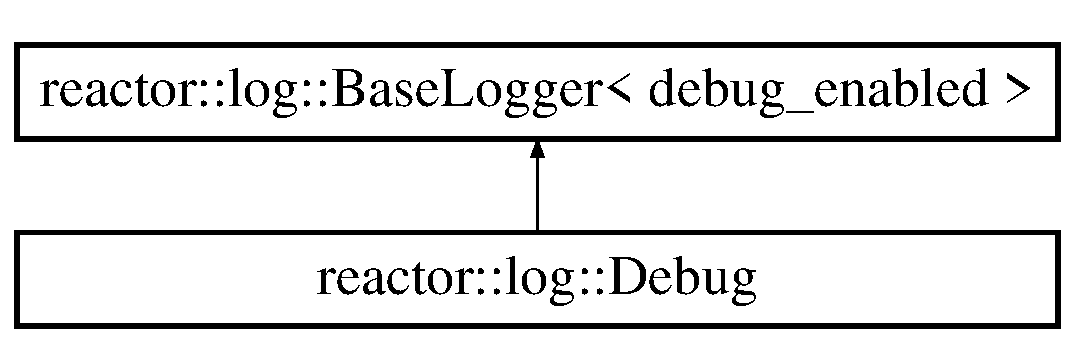
\includegraphics[height=2.000000cm]{structreactor_1_1log_1_1Debug}
\end{center}
\end{figure}
\subsection*{Public Member Functions}
\begin{DoxyCompactItemize}
\item 
\hyperlink{structreactor_1_1log_1_1Debug_a7675a74aaae5b2c062dfd88840b7c1ac}{Debug} ()
\end{DoxyCompactItemize}


\subsection{Constructor \& Destructor Documentation}
\mbox{\Hypertarget{structreactor_1_1log_1_1Debug_a7675a74aaae5b2c062dfd88840b7c1ac}\label{structreactor_1_1log_1_1Debug_a7675a74aaae5b2c062dfd88840b7c1ac}} 
\index{reactor\+::log\+::\+Debug@{reactor\+::log\+::\+Debug}!Debug@{Debug}}
\index{Debug@{Debug}!reactor\+::log\+::\+Debug@{reactor\+::log\+::\+Debug}}
\subsubsection{\texorpdfstring{Debug()}{Debug()}}
{\footnotesize\ttfamily reactor\+::log\+::\+Debug\+::\+Debug (\begin{DoxyParamCaption}{ }\end{DoxyParamCaption})\hspace{0.3cm}{\ttfamily [inline]}}



The documentation for this struct was generated from the following file\+:\begin{DoxyCompactItemize}
\item 
/home/runner/work/reactor-\/cpp/reactor-\/cpp/include/reactor-\/cpp/\hyperlink{logging_8hh}{logging.\+hh}\end{DoxyCompactItemize}

\hypertarget{classreactor_1_1Environment}{}\section{reactor\+:\+:Environment Class Reference}
\label{classreactor_1_1Environment}\index{reactor\+::\+Environment@{reactor\+::\+Environment}}


{\ttfamily \#include $<$environment.\+hh$>$}

\subsection*{Public Types}
\begin{DoxyCompactItemize}
\item 
enum \hyperlink{classreactor_1_1Environment_a2f0bcf10490e174246fc14b456fb0755}{Phase} \{ \newline
\hyperlink{classreactor_1_1Environment_a2f0bcf10490e174246fc14b456fb0755a2a0d30cb1153031c3dfc239c6e0407ea}{Phase\+::\+Construction}, 
\hyperlink{classreactor_1_1Environment_a2f0bcf10490e174246fc14b456fb0755ad75c45e11c8aeb13494dba59a388a164}{Phase\+::\+Assembly}, 
\hyperlink{classreactor_1_1Environment_a2f0bcf10490e174246fc14b456fb0755a13e685964c2548aa748f7ea263bad4e5}{Phase\+::\+Startup}, 
\hyperlink{classreactor_1_1Environment_a2f0bcf10490e174246fc14b456fb0755a8f44785c8c19412c5b6611db30984514}{Phase\+::\+Execution}, 
\newline
\hyperlink{classreactor_1_1Environment_a2f0bcf10490e174246fc14b456fb0755a1a4ebb180ba59b067782515ffee6e975}{Phase\+::\+Shutdown}, 
\hyperlink{classreactor_1_1Environment_a2f0bcf10490e174246fc14b456fb0755a7629cb3f7fc48e33116e336bdfd141fd}{Phase\+::\+Deconstruction}
 \}
\end{DoxyCompactItemize}
\subsection*{Public Member Functions}
\begin{DoxyCompactItemize}
\item 
\hyperlink{classreactor_1_1Environment_add3e14bfed87d544bac849fced7f30f8}{Environment} (unsigned \hyperlink{classreactor_1_1Environment_a3348b53c1d45a315920832d7505f9057}{num\+\_\+workers}, bool \hyperlink{classreactor_1_1Environment_a7a83a769b141d23297912e7588eb4495}{run\+\_\+forever}=false, bool \hyperlink{classreactor_1_1Environment_a4f6e899d401fc1238143de9d725c247d}{fast\+\_\+fwd\+\_\+execution}=false)
\item 
void \hyperlink{classreactor_1_1Environment_afa74eb3e5dd5a7a4b1629f9dd63a168f}{register\+\_\+reactor} (\hyperlink{classreactor_1_1Reactor}{Reactor} $\ast$reactor)
\item 
const auto \& \hyperlink{classreactor_1_1Environment_a89de40b92defdcde2e090a6f244c1eab}{top\+\_\+level\+\_\+reactors} () const
\item 
void \hyperlink{classreactor_1_1Environment_afd2ce93dd4fae7a1c6c93a8a274bf618}{assemble} ()
\item 
std\+::thread \hyperlink{classreactor_1_1Environment_a978f39f3609ed3889db10961505a61d9}{startup} ()
\item 
void \hyperlink{classreactor_1_1Environment_a7bc165b2d7a3a6bc6c4573c26170dc50}{sync\+\_\+shutdown} ()
\item 
void \hyperlink{classreactor_1_1Environment_a78cc13dcc68f71867e967da1c7cca001}{async\+\_\+shutdown} ()
\item 
void \hyperlink{classreactor_1_1Environment_a5f80b554cf21643375ad1202c8aea85c}{export\+\_\+dependency\+\_\+graph} (const std\+::string \&path)
\item 
\hyperlink{classreactor_1_1Environment_a2f0bcf10490e174246fc14b456fb0755}{Phase} \hyperlink{classreactor_1_1Environment_ab0cc703268b97b54e0a9e0927f0738d4}{phase} () const
\item 
const \hyperlink{classreactor_1_1Scheduler}{Scheduler} $\ast$ \hyperlink{classreactor_1_1Environment_a2a4cf2150b314a18db041e8a06086904}{scheduler} () const
\item 
\hyperlink{classreactor_1_1Scheduler}{Scheduler} $\ast$ \hyperlink{classreactor_1_1Environment_a4ac32b7f7f9a420bb689d7f5c5ce48da}{scheduler} ()
\item 
const \hyperlink{classreactor_1_1LogicalTime}{Logical\+Time} \& \hyperlink{classreactor_1_1Environment_a09aa23da721fffd3bb0b62f879d167b0}{logical\+\_\+time} () const
\item 
const \hyperlink{namespacereactor_ad950f8d1a46612500286a4af0f167080}{Time\+Point} \& \hyperlink{classreactor_1_1Environment_af7643c6bf796bd083ff4976af19e8838}{start\+\_\+time} () const
\item 
\hyperlink{namespacereactor_ad950f8d1a46612500286a4af0f167080}{Time\+Point} \hyperlink{classreactor_1_1Environment_aaf28ead7b6e2a273f000f71524d81a11}{physical\+\_\+time} () const
\item 
unsigned \hyperlink{classreactor_1_1Environment_a3348b53c1d45a315920832d7505f9057}{num\+\_\+workers} () const
\item 
bool \hyperlink{classreactor_1_1Environment_a4f6e899d401fc1238143de9d725c247d}{fast\+\_\+fwd\+\_\+execution} () const
\item 
bool \hyperlink{classreactor_1_1Environment_a7a83a769b141d23297912e7588eb4495}{run\+\_\+forever} () const
\item 
unsigned \hyperlink{classreactor_1_1Environment_a2d50de0d09d5aa56a9876441233590f0}{max\+\_\+reaction\+\_\+index} () const
\end{DoxyCompactItemize}
\subsection*{Private Types}
\begin{DoxyCompactItemize}
\item 
using \hyperlink{classreactor_1_1Environment_aefeb24b3f7a321c7dc8309cac1ed176d}{Dependency} = std\+::pair$<$ \hyperlink{classreactor_1_1Reaction}{Reaction} $\ast$, \hyperlink{classreactor_1_1Reaction}{Reaction} $\ast$ $>$
\end{DoxyCompactItemize}
\subsection*{Private Member Functions}
\begin{DoxyCompactItemize}
\item 
void \hyperlink{classreactor_1_1Environment_a25e3210c41ddd193223c63adc454358a}{build\+\_\+dependency\+\_\+graph} (\hyperlink{classreactor_1_1Reactor}{Reactor} $\ast$reactor)
\item 
void \hyperlink{classreactor_1_1Environment_a8b832858f8c20d36ffc8331ef9f9ac14}{calculate\+\_\+indexes} ()
\end{DoxyCompactItemize}
\subsection*{Private Attributes}
\begin{DoxyCompactItemize}
\item 
const unsigned \hyperlink{classreactor_1_1Environment_a01fac164f06a9f97bb2ee5b0b6d4a368}{\+\_\+num\+\_\+workers}
\item 
\hyperlink{classreactor_1_1Scheduler}{Scheduler} \hyperlink{classreactor_1_1Environment_ae07319eb6bc85a9c00ac324db4891217}{\+\_\+scheduler}
\item 
const bool \hyperlink{classreactor_1_1Environment_ad842507a720c670f9a51dbee020ed08b}{\+\_\+run\+\_\+forever}
\item 
const bool \hyperlink{classreactor_1_1Environment_ad49bd4d74a5fdf2132a4ca9933135b99}{\+\_\+fast\+\_\+fwd\+\_\+execution}
\item 
std\+::set$<$ \hyperlink{classreactor_1_1Reactor}{Reactor} $\ast$ $>$ \hyperlink{classreactor_1_1Environment_a15707bfeefc0200d2956e3b52c8270db}{\+\_\+top\+\_\+level\+\_\+reactors}
\item 
std\+::set$<$ \hyperlink{classreactor_1_1Reaction}{Reaction} $\ast$ $>$ \hyperlink{classreactor_1_1Environment_abaca5b55047bbf45f4280eeeb8cd38c4}{reactions}
\item 
std\+::vector$<$ \hyperlink{classreactor_1_1Environment_aefeb24b3f7a321c7dc8309cac1ed176d}{Dependency} $>$ \hyperlink{classreactor_1_1Environment_ac67e4fbe9d7365e4570fc9667c003f41}{dependencies}
\item 
\hyperlink{classreactor_1_1Environment_a2f0bcf10490e174246fc14b456fb0755}{Phase} \hyperlink{classreactor_1_1Environment_a15d6118f5ae312ad7665418969cc831a}{\+\_\+phase} \{\hyperlink{classreactor_1_1Environment_a2f0bcf10490e174246fc14b456fb0755a2a0d30cb1153031c3dfc239c6e0407ea}{Phase\+::\+Construction}\}
\item 
\hyperlink{namespacereactor_ad950f8d1a46612500286a4af0f167080}{Time\+Point} \hyperlink{classreactor_1_1Environment_adcc50c30d8fb1ad1dca3033e6819e3b8}{\+\_\+start\+\_\+time}
\item 
unsigned \hyperlink{classreactor_1_1Environment_aaacf54f45077c2c90e2c2ba628f088e8}{\+\_\+max\+\_\+reaction\+\_\+index}
\end{DoxyCompactItemize}


\subsection{Member Typedef Documentation}
\mbox{\Hypertarget{classreactor_1_1Environment_aefeb24b3f7a321c7dc8309cac1ed176d}\label{classreactor_1_1Environment_aefeb24b3f7a321c7dc8309cac1ed176d}} 
\index{reactor\+::\+Environment@{reactor\+::\+Environment}!Dependency@{Dependency}}
\index{Dependency@{Dependency}!reactor\+::\+Environment@{reactor\+::\+Environment}}
\subsubsection{\texorpdfstring{Dependency}{Dependency}}
{\footnotesize\ttfamily using \hyperlink{classreactor_1_1Environment_aefeb24b3f7a321c7dc8309cac1ed176d}{reactor\+::\+Environment\+::\+Dependency} =  std\+::pair$<$\hyperlink{classreactor_1_1Reaction}{Reaction}$\ast$, \hyperlink{classreactor_1_1Reaction}{Reaction}$\ast$$>$\hspace{0.3cm}{\ttfamily [private]}}



\subsection{Member Enumeration Documentation}
\mbox{\Hypertarget{classreactor_1_1Environment_a2f0bcf10490e174246fc14b456fb0755}\label{classreactor_1_1Environment_a2f0bcf10490e174246fc14b456fb0755}} 
\index{reactor\+::\+Environment@{reactor\+::\+Environment}!Phase@{Phase}}
\index{Phase@{Phase}!reactor\+::\+Environment@{reactor\+::\+Environment}}
\subsubsection{\texorpdfstring{Phase}{Phase}}
{\footnotesize\ttfamily enum \hyperlink{classreactor_1_1Environment_a2f0bcf10490e174246fc14b456fb0755}{reactor\+::\+Environment\+::\+Phase}\hspace{0.3cm}{\ttfamily [strong]}}

\begin{DoxyEnumFields}{Enumerator}
\raisebox{\heightof{T}}[0pt][0pt]{\index{Construction@{Construction}!reactor\+::\+Environment@{reactor\+::\+Environment}}\index{reactor\+::\+Environment@{reactor\+::\+Environment}!Construction@{Construction}}}\mbox{\Hypertarget{classreactor_1_1Environment_a2f0bcf10490e174246fc14b456fb0755a2a0d30cb1153031c3dfc239c6e0407ea}\label{classreactor_1_1Environment_a2f0bcf10490e174246fc14b456fb0755a2a0d30cb1153031c3dfc239c6e0407ea}} 
Construction&\\
\hline

\raisebox{\heightof{T}}[0pt][0pt]{\index{Assembly@{Assembly}!reactor\+::\+Environment@{reactor\+::\+Environment}}\index{reactor\+::\+Environment@{reactor\+::\+Environment}!Assembly@{Assembly}}}\mbox{\Hypertarget{classreactor_1_1Environment_a2f0bcf10490e174246fc14b456fb0755ad75c45e11c8aeb13494dba59a388a164}\label{classreactor_1_1Environment_a2f0bcf10490e174246fc14b456fb0755ad75c45e11c8aeb13494dba59a388a164}} 
Assembly&\\
\hline

\raisebox{\heightof{T}}[0pt][0pt]{\index{Startup@{Startup}!reactor\+::\+Environment@{reactor\+::\+Environment}}\index{reactor\+::\+Environment@{reactor\+::\+Environment}!Startup@{Startup}}}\mbox{\Hypertarget{classreactor_1_1Environment_a2f0bcf10490e174246fc14b456fb0755a13e685964c2548aa748f7ea263bad4e5}\label{classreactor_1_1Environment_a2f0bcf10490e174246fc14b456fb0755a13e685964c2548aa748f7ea263bad4e5}} 
Startup&\\
\hline

\raisebox{\heightof{T}}[0pt][0pt]{\index{Execution@{Execution}!reactor\+::\+Environment@{reactor\+::\+Environment}}\index{reactor\+::\+Environment@{reactor\+::\+Environment}!Execution@{Execution}}}\mbox{\Hypertarget{classreactor_1_1Environment_a2f0bcf10490e174246fc14b456fb0755a8f44785c8c19412c5b6611db30984514}\label{classreactor_1_1Environment_a2f0bcf10490e174246fc14b456fb0755a8f44785c8c19412c5b6611db30984514}} 
Execution&\\
\hline

\raisebox{\heightof{T}}[0pt][0pt]{\index{Shutdown@{Shutdown}!reactor\+::\+Environment@{reactor\+::\+Environment}}\index{reactor\+::\+Environment@{reactor\+::\+Environment}!Shutdown@{Shutdown}}}\mbox{\Hypertarget{classreactor_1_1Environment_a2f0bcf10490e174246fc14b456fb0755a1a4ebb180ba59b067782515ffee6e975}\label{classreactor_1_1Environment_a2f0bcf10490e174246fc14b456fb0755a1a4ebb180ba59b067782515ffee6e975}} 
Shutdown&\\
\hline

\raisebox{\heightof{T}}[0pt][0pt]{\index{Deconstruction@{Deconstruction}!reactor\+::\+Environment@{reactor\+::\+Environment}}\index{reactor\+::\+Environment@{reactor\+::\+Environment}!Deconstruction@{Deconstruction}}}\mbox{\Hypertarget{classreactor_1_1Environment_a2f0bcf10490e174246fc14b456fb0755a7629cb3f7fc48e33116e336bdfd141fd}\label{classreactor_1_1Environment_a2f0bcf10490e174246fc14b456fb0755a7629cb3f7fc48e33116e336bdfd141fd}} 
Deconstruction&\\
\hline

\end{DoxyEnumFields}


\subsection{Constructor \& Destructor Documentation}
\mbox{\Hypertarget{classreactor_1_1Environment_add3e14bfed87d544bac849fced7f30f8}\label{classreactor_1_1Environment_add3e14bfed87d544bac849fced7f30f8}} 
\index{reactor\+::\+Environment@{reactor\+::\+Environment}!Environment@{Environment}}
\index{Environment@{Environment}!reactor\+::\+Environment@{reactor\+::\+Environment}}
\subsubsection{\texorpdfstring{Environment()}{Environment()}}
{\footnotesize\ttfamily reactor\+::\+Environment\+::\+Environment (\begin{DoxyParamCaption}\item[{unsigned}]{num\+\_\+workers,  }\item[{bool}]{run\+\_\+forever = {\ttfamily false},  }\item[{bool}]{fast\+\_\+fwd\+\_\+execution = {\ttfamily false} }\end{DoxyParamCaption})\hspace{0.3cm}{\ttfamily [inline]}}



\subsection{Member Function Documentation}
\mbox{\Hypertarget{classreactor_1_1Environment_afd2ce93dd4fae7a1c6c93a8a274bf618}\label{classreactor_1_1Environment_afd2ce93dd4fae7a1c6c93a8a274bf618}} 
\index{reactor\+::\+Environment@{reactor\+::\+Environment}!assemble@{assemble}}
\index{assemble@{assemble}!reactor\+::\+Environment@{reactor\+::\+Environment}}
\subsubsection{\texorpdfstring{assemble()}{assemble()}}
{\footnotesize\ttfamily void reactor\+::\+Environment\+::assemble (\begin{DoxyParamCaption}{ }\end{DoxyParamCaption})}

\mbox{\Hypertarget{classreactor_1_1Environment_a78cc13dcc68f71867e967da1c7cca001}\label{classreactor_1_1Environment_a78cc13dcc68f71867e967da1c7cca001}} 
\index{reactor\+::\+Environment@{reactor\+::\+Environment}!async\+\_\+shutdown@{async\+\_\+shutdown}}
\index{async\+\_\+shutdown@{async\+\_\+shutdown}!reactor\+::\+Environment@{reactor\+::\+Environment}}
\subsubsection{\texorpdfstring{async\+\_\+shutdown()}{async\_shutdown()}}
{\footnotesize\ttfamily void reactor\+::\+Environment\+::async\+\_\+shutdown (\begin{DoxyParamCaption}{ }\end{DoxyParamCaption})}

\mbox{\Hypertarget{classreactor_1_1Environment_a25e3210c41ddd193223c63adc454358a}\label{classreactor_1_1Environment_a25e3210c41ddd193223c63adc454358a}} 
\index{reactor\+::\+Environment@{reactor\+::\+Environment}!build\+\_\+dependency\+\_\+graph@{build\+\_\+dependency\+\_\+graph}}
\index{build\+\_\+dependency\+\_\+graph@{build\+\_\+dependency\+\_\+graph}!reactor\+::\+Environment@{reactor\+::\+Environment}}
\subsubsection{\texorpdfstring{build\+\_\+dependency\+\_\+graph()}{build\_dependency\_graph()}}
{\footnotesize\ttfamily void reactor\+::\+Environment\+::build\+\_\+dependency\+\_\+graph (\begin{DoxyParamCaption}\item[{\hyperlink{classreactor_1_1Reactor}{Reactor} $\ast$}]{reactor }\end{DoxyParamCaption})\hspace{0.3cm}{\ttfamily [private]}}

\mbox{\Hypertarget{classreactor_1_1Environment_a8b832858f8c20d36ffc8331ef9f9ac14}\label{classreactor_1_1Environment_a8b832858f8c20d36ffc8331ef9f9ac14}} 
\index{reactor\+::\+Environment@{reactor\+::\+Environment}!calculate\+\_\+indexes@{calculate\+\_\+indexes}}
\index{calculate\+\_\+indexes@{calculate\+\_\+indexes}!reactor\+::\+Environment@{reactor\+::\+Environment}}
\subsubsection{\texorpdfstring{calculate\+\_\+indexes()}{calculate\_indexes()}}
{\footnotesize\ttfamily void reactor\+::\+Environment\+::calculate\+\_\+indexes (\begin{DoxyParamCaption}{ }\end{DoxyParamCaption})\hspace{0.3cm}{\ttfamily [private]}}

\mbox{\Hypertarget{classreactor_1_1Environment_a5f80b554cf21643375ad1202c8aea85c}\label{classreactor_1_1Environment_a5f80b554cf21643375ad1202c8aea85c}} 
\index{reactor\+::\+Environment@{reactor\+::\+Environment}!export\+\_\+dependency\+\_\+graph@{export\+\_\+dependency\+\_\+graph}}
\index{export\+\_\+dependency\+\_\+graph@{export\+\_\+dependency\+\_\+graph}!reactor\+::\+Environment@{reactor\+::\+Environment}}
\subsubsection{\texorpdfstring{export\+\_\+dependency\+\_\+graph()}{export\_dependency\_graph()}}
{\footnotesize\ttfamily void reactor\+::\+Environment\+::export\+\_\+dependency\+\_\+graph (\begin{DoxyParamCaption}\item[{const std\+::string \&}]{path }\end{DoxyParamCaption})}

\mbox{\Hypertarget{classreactor_1_1Environment_a4f6e899d401fc1238143de9d725c247d}\label{classreactor_1_1Environment_a4f6e899d401fc1238143de9d725c247d}} 
\index{reactor\+::\+Environment@{reactor\+::\+Environment}!fast\+\_\+fwd\+\_\+execution@{fast\+\_\+fwd\+\_\+execution}}
\index{fast\+\_\+fwd\+\_\+execution@{fast\+\_\+fwd\+\_\+execution}!reactor\+::\+Environment@{reactor\+::\+Environment}}
\subsubsection{\texorpdfstring{fast\+\_\+fwd\+\_\+execution()}{fast\_fwd\_execution()}}
{\footnotesize\ttfamily bool reactor\+::\+Environment\+::fast\+\_\+fwd\+\_\+execution (\begin{DoxyParamCaption}{ }\end{DoxyParamCaption}) const\hspace{0.3cm}{\ttfamily [inline]}}

\mbox{\Hypertarget{classreactor_1_1Environment_a09aa23da721fffd3bb0b62f879d167b0}\label{classreactor_1_1Environment_a09aa23da721fffd3bb0b62f879d167b0}} 
\index{reactor\+::\+Environment@{reactor\+::\+Environment}!logical\+\_\+time@{logical\+\_\+time}}
\index{logical\+\_\+time@{logical\+\_\+time}!reactor\+::\+Environment@{reactor\+::\+Environment}}
\subsubsection{\texorpdfstring{logical\+\_\+time()}{logical\_time()}}
{\footnotesize\ttfamily const \hyperlink{classreactor_1_1LogicalTime}{Logical\+Time}\& reactor\+::\+Environment\+::logical\+\_\+time (\begin{DoxyParamCaption}{ }\end{DoxyParamCaption}) const\hspace{0.3cm}{\ttfamily [inline]}}

\mbox{\Hypertarget{classreactor_1_1Environment_a2d50de0d09d5aa56a9876441233590f0}\label{classreactor_1_1Environment_a2d50de0d09d5aa56a9876441233590f0}} 
\index{reactor\+::\+Environment@{reactor\+::\+Environment}!max\+\_\+reaction\+\_\+index@{max\+\_\+reaction\+\_\+index}}
\index{max\+\_\+reaction\+\_\+index@{max\+\_\+reaction\+\_\+index}!reactor\+::\+Environment@{reactor\+::\+Environment}}
\subsubsection{\texorpdfstring{max\+\_\+reaction\+\_\+index()}{max\_reaction\_index()}}
{\footnotesize\ttfamily unsigned reactor\+::\+Environment\+::max\+\_\+reaction\+\_\+index (\begin{DoxyParamCaption}{ }\end{DoxyParamCaption}) const\hspace{0.3cm}{\ttfamily [inline]}}

\mbox{\Hypertarget{classreactor_1_1Environment_a3348b53c1d45a315920832d7505f9057}\label{classreactor_1_1Environment_a3348b53c1d45a315920832d7505f9057}} 
\index{reactor\+::\+Environment@{reactor\+::\+Environment}!num\+\_\+workers@{num\+\_\+workers}}
\index{num\+\_\+workers@{num\+\_\+workers}!reactor\+::\+Environment@{reactor\+::\+Environment}}
\subsubsection{\texorpdfstring{num\+\_\+workers()}{num\_workers()}}
{\footnotesize\ttfamily unsigned reactor\+::\+Environment\+::num\+\_\+workers (\begin{DoxyParamCaption}{ }\end{DoxyParamCaption}) const\hspace{0.3cm}{\ttfamily [inline]}}

\mbox{\Hypertarget{classreactor_1_1Environment_ab0cc703268b97b54e0a9e0927f0738d4}\label{classreactor_1_1Environment_ab0cc703268b97b54e0a9e0927f0738d4}} 
\index{reactor\+::\+Environment@{reactor\+::\+Environment}!phase@{phase}}
\index{phase@{phase}!reactor\+::\+Environment@{reactor\+::\+Environment}}
\subsubsection{\texorpdfstring{phase()}{phase()}}
{\footnotesize\ttfamily \hyperlink{classreactor_1_1Environment_a2f0bcf10490e174246fc14b456fb0755}{Phase} reactor\+::\+Environment\+::phase (\begin{DoxyParamCaption}{ }\end{DoxyParamCaption}) const\hspace{0.3cm}{\ttfamily [inline]}}

\mbox{\Hypertarget{classreactor_1_1Environment_aaf28ead7b6e2a273f000f71524d81a11}\label{classreactor_1_1Environment_aaf28ead7b6e2a273f000f71524d81a11}} 
\index{reactor\+::\+Environment@{reactor\+::\+Environment}!physical\+\_\+time@{physical\+\_\+time}}
\index{physical\+\_\+time@{physical\+\_\+time}!reactor\+::\+Environment@{reactor\+::\+Environment}}
\subsubsection{\texorpdfstring{physical\+\_\+time()}{physical\_time()}}
{\footnotesize\ttfamily \hyperlink{namespacereactor_ad950f8d1a46612500286a4af0f167080}{Time\+Point} reactor\+::\+Environment\+::physical\+\_\+time (\begin{DoxyParamCaption}{ }\end{DoxyParamCaption}) const\hspace{0.3cm}{\ttfamily [inline]}}

\mbox{\Hypertarget{classreactor_1_1Environment_afa74eb3e5dd5a7a4b1629f9dd63a168f}\label{classreactor_1_1Environment_afa74eb3e5dd5a7a4b1629f9dd63a168f}} 
\index{reactor\+::\+Environment@{reactor\+::\+Environment}!register\+\_\+reactor@{register\+\_\+reactor}}
\index{register\+\_\+reactor@{register\+\_\+reactor}!reactor\+::\+Environment@{reactor\+::\+Environment}}
\subsubsection{\texorpdfstring{register\+\_\+reactor()}{register\_reactor()}}
{\footnotesize\ttfamily void reactor\+::\+Environment\+::register\+\_\+reactor (\begin{DoxyParamCaption}\item[{\hyperlink{classreactor_1_1Reactor}{Reactor} $\ast$}]{reactor }\end{DoxyParamCaption})}

\mbox{\Hypertarget{classreactor_1_1Environment_a7a83a769b141d23297912e7588eb4495}\label{classreactor_1_1Environment_a7a83a769b141d23297912e7588eb4495}} 
\index{reactor\+::\+Environment@{reactor\+::\+Environment}!run\+\_\+forever@{run\+\_\+forever}}
\index{run\+\_\+forever@{run\+\_\+forever}!reactor\+::\+Environment@{reactor\+::\+Environment}}
\subsubsection{\texorpdfstring{run\+\_\+forever()}{run\_forever()}}
{\footnotesize\ttfamily bool reactor\+::\+Environment\+::run\+\_\+forever (\begin{DoxyParamCaption}{ }\end{DoxyParamCaption}) const\hspace{0.3cm}{\ttfamily [inline]}}

\mbox{\Hypertarget{classreactor_1_1Environment_a2a4cf2150b314a18db041e8a06086904}\label{classreactor_1_1Environment_a2a4cf2150b314a18db041e8a06086904}} 
\index{reactor\+::\+Environment@{reactor\+::\+Environment}!scheduler@{scheduler}}
\index{scheduler@{scheduler}!reactor\+::\+Environment@{reactor\+::\+Environment}}
\subsubsection{\texorpdfstring{scheduler()}{scheduler()}\hspace{0.1cm}{\footnotesize\ttfamily [1/2]}}
{\footnotesize\ttfamily const \hyperlink{classreactor_1_1Scheduler}{Scheduler}$\ast$ reactor\+::\+Environment\+::scheduler (\begin{DoxyParamCaption}{ }\end{DoxyParamCaption}) const\hspace{0.3cm}{\ttfamily [inline]}}

\mbox{\Hypertarget{classreactor_1_1Environment_a4ac32b7f7f9a420bb689d7f5c5ce48da}\label{classreactor_1_1Environment_a4ac32b7f7f9a420bb689d7f5c5ce48da}} 
\index{reactor\+::\+Environment@{reactor\+::\+Environment}!scheduler@{scheduler}}
\index{scheduler@{scheduler}!reactor\+::\+Environment@{reactor\+::\+Environment}}
\subsubsection{\texorpdfstring{scheduler()}{scheduler()}\hspace{0.1cm}{\footnotesize\ttfamily [2/2]}}
{\footnotesize\ttfamily \hyperlink{classreactor_1_1Scheduler}{Scheduler}$\ast$ reactor\+::\+Environment\+::scheduler (\begin{DoxyParamCaption}{ }\end{DoxyParamCaption})\hspace{0.3cm}{\ttfamily [inline]}}

\mbox{\Hypertarget{classreactor_1_1Environment_af7643c6bf796bd083ff4976af19e8838}\label{classreactor_1_1Environment_af7643c6bf796bd083ff4976af19e8838}} 
\index{reactor\+::\+Environment@{reactor\+::\+Environment}!start\+\_\+time@{start\+\_\+time}}
\index{start\+\_\+time@{start\+\_\+time}!reactor\+::\+Environment@{reactor\+::\+Environment}}
\subsubsection{\texorpdfstring{start\+\_\+time()}{start\_time()}}
{\footnotesize\ttfamily const \hyperlink{namespacereactor_ad950f8d1a46612500286a4af0f167080}{Time\+Point}\& reactor\+::\+Environment\+::start\+\_\+time (\begin{DoxyParamCaption}{ }\end{DoxyParamCaption}) const\hspace{0.3cm}{\ttfamily [inline]}}

\mbox{\Hypertarget{classreactor_1_1Environment_a978f39f3609ed3889db10961505a61d9}\label{classreactor_1_1Environment_a978f39f3609ed3889db10961505a61d9}} 
\index{reactor\+::\+Environment@{reactor\+::\+Environment}!startup@{startup}}
\index{startup@{startup}!reactor\+::\+Environment@{reactor\+::\+Environment}}
\subsubsection{\texorpdfstring{startup()}{startup()}}
{\footnotesize\ttfamily std\+::thread reactor\+::\+Environment\+::startup (\begin{DoxyParamCaption}{ }\end{DoxyParamCaption})}

\mbox{\Hypertarget{classreactor_1_1Environment_a7bc165b2d7a3a6bc6c4573c26170dc50}\label{classreactor_1_1Environment_a7bc165b2d7a3a6bc6c4573c26170dc50}} 
\index{reactor\+::\+Environment@{reactor\+::\+Environment}!sync\+\_\+shutdown@{sync\+\_\+shutdown}}
\index{sync\+\_\+shutdown@{sync\+\_\+shutdown}!reactor\+::\+Environment@{reactor\+::\+Environment}}
\subsubsection{\texorpdfstring{sync\+\_\+shutdown()}{sync\_shutdown()}}
{\footnotesize\ttfamily void reactor\+::\+Environment\+::sync\+\_\+shutdown (\begin{DoxyParamCaption}{ }\end{DoxyParamCaption})}

\mbox{\Hypertarget{classreactor_1_1Environment_a89de40b92defdcde2e090a6f244c1eab}\label{classreactor_1_1Environment_a89de40b92defdcde2e090a6f244c1eab}} 
\index{reactor\+::\+Environment@{reactor\+::\+Environment}!top\+\_\+level\+\_\+reactors@{top\+\_\+level\+\_\+reactors}}
\index{top\+\_\+level\+\_\+reactors@{top\+\_\+level\+\_\+reactors}!reactor\+::\+Environment@{reactor\+::\+Environment}}
\subsubsection{\texorpdfstring{top\+\_\+level\+\_\+reactors()}{top\_level\_reactors()}}
{\footnotesize\ttfamily const auto\& reactor\+::\+Environment\+::top\+\_\+level\+\_\+reactors (\begin{DoxyParamCaption}{ }\end{DoxyParamCaption}) const\hspace{0.3cm}{\ttfamily [inline]}}



\subsection{Member Data Documentation}
\mbox{\Hypertarget{classreactor_1_1Environment_ad49bd4d74a5fdf2132a4ca9933135b99}\label{classreactor_1_1Environment_ad49bd4d74a5fdf2132a4ca9933135b99}} 
\index{reactor\+::\+Environment@{reactor\+::\+Environment}!\+\_\+fast\+\_\+fwd\+\_\+execution@{\+\_\+fast\+\_\+fwd\+\_\+execution}}
\index{\+\_\+fast\+\_\+fwd\+\_\+execution@{\+\_\+fast\+\_\+fwd\+\_\+execution}!reactor\+::\+Environment@{reactor\+::\+Environment}}
\subsubsection{\texorpdfstring{\+\_\+fast\+\_\+fwd\+\_\+execution}{\_fast\_fwd\_execution}}
{\footnotesize\ttfamily const bool reactor\+::\+Environment\+::\+\_\+fast\+\_\+fwd\+\_\+execution\hspace{0.3cm}{\ttfamily [private]}}

\mbox{\Hypertarget{classreactor_1_1Environment_aaacf54f45077c2c90e2c2ba628f088e8}\label{classreactor_1_1Environment_aaacf54f45077c2c90e2c2ba628f088e8}} 
\index{reactor\+::\+Environment@{reactor\+::\+Environment}!\+\_\+max\+\_\+reaction\+\_\+index@{\+\_\+max\+\_\+reaction\+\_\+index}}
\index{\+\_\+max\+\_\+reaction\+\_\+index@{\+\_\+max\+\_\+reaction\+\_\+index}!reactor\+::\+Environment@{reactor\+::\+Environment}}
\subsubsection{\texorpdfstring{\+\_\+max\+\_\+reaction\+\_\+index}{\_max\_reaction\_index}}
{\footnotesize\ttfamily unsigned reactor\+::\+Environment\+::\+\_\+max\+\_\+reaction\+\_\+index\hspace{0.3cm}{\ttfamily [private]}}

\mbox{\Hypertarget{classreactor_1_1Environment_a01fac164f06a9f97bb2ee5b0b6d4a368}\label{classreactor_1_1Environment_a01fac164f06a9f97bb2ee5b0b6d4a368}} 
\index{reactor\+::\+Environment@{reactor\+::\+Environment}!\+\_\+num\+\_\+workers@{\+\_\+num\+\_\+workers}}
\index{\+\_\+num\+\_\+workers@{\+\_\+num\+\_\+workers}!reactor\+::\+Environment@{reactor\+::\+Environment}}
\subsubsection{\texorpdfstring{\+\_\+num\+\_\+workers}{\_num\_workers}}
{\footnotesize\ttfamily const unsigned reactor\+::\+Environment\+::\+\_\+num\+\_\+workers\hspace{0.3cm}{\ttfamily [private]}}

\mbox{\Hypertarget{classreactor_1_1Environment_a15d6118f5ae312ad7665418969cc831a}\label{classreactor_1_1Environment_a15d6118f5ae312ad7665418969cc831a}} 
\index{reactor\+::\+Environment@{reactor\+::\+Environment}!\+\_\+phase@{\+\_\+phase}}
\index{\+\_\+phase@{\+\_\+phase}!reactor\+::\+Environment@{reactor\+::\+Environment}}
\subsubsection{\texorpdfstring{\+\_\+phase}{\_phase}}
{\footnotesize\ttfamily \hyperlink{classreactor_1_1Environment_a2f0bcf10490e174246fc14b456fb0755}{Phase} reactor\+::\+Environment\+::\+\_\+phase \{\hyperlink{classreactor_1_1Environment_a2f0bcf10490e174246fc14b456fb0755a2a0d30cb1153031c3dfc239c6e0407ea}{Phase\+::\+Construction}\}\hspace{0.3cm}{\ttfamily [private]}}

\mbox{\Hypertarget{classreactor_1_1Environment_ad842507a720c670f9a51dbee020ed08b}\label{classreactor_1_1Environment_ad842507a720c670f9a51dbee020ed08b}} 
\index{reactor\+::\+Environment@{reactor\+::\+Environment}!\+\_\+run\+\_\+forever@{\+\_\+run\+\_\+forever}}
\index{\+\_\+run\+\_\+forever@{\+\_\+run\+\_\+forever}!reactor\+::\+Environment@{reactor\+::\+Environment}}
\subsubsection{\texorpdfstring{\+\_\+run\+\_\+forever}{\_run\_forever}}
{\footnotesize\ttfamily const bool reactor\+::\+Environment\+::\+\_\+run\+\_\+forever\hspace{0.3cm}{\ttfamily [private]}}

\mbox{\Hypertarget{classreactor_1_1Environment_ae07319eb6bc85a9c00ac324db4891217}\label{classreactor_1_1Environment_ae07319eb6bc85a9c00ac324db4891217}} 
\index{reactor\+::\+Environment@{reactor\+::\+Environment}!\+\_\+scheduler@{\+\_\+scheduler}}
\index{\+\_\+scheduler@{\+\_\+scheduler}!reactor\+::\+Environment@{reactor\+::\+Environment}}
\subsubsection{\texorpdfstring{\+\_\+scheduler}{\_scheduler}}
{\footnotesize\ttfamily \hyperlink{classreactor_1_1Scheduler}{Scheduler} reactor\+::\+Environment\+::\+\_\+scheduler\hspace{0.3cm}{\ttfamily [private]}}

\mbox{\Hypertarget{classreactor_1_1Environment_adcc50c30d8fb1ad1dca3033e6819e3b8}\label{classreactor_1_1Environment_adcc50c30d8fb1ad1dca3033e6819e3b8}} 
\index{reactor\+::\+Environment@{reactor\+::\+Environment}!\+\_\+start\+\_\+time@{\+\_\+start\+\_\+time}}
\index{\+\_\+start\+\_\+time@{\+\_\+start\+\_\+time}!reactor\+::\+Environment@{reactor\+::\+Environment}}
\subsubsection{\texorpdfstring{\+\_\+start\+\_\+time}{\_start\_time}}
{\footnotesize\ttfamily \hyperlink{namespacereactor_ad950f8d1a46612500286a4af0f167080}{Time\+Point} reactor\+::\+Environment\+::\+\_\+start\+\_\+time\hspace{0.3cm}{\ttfamily [private]}}

\mbox{\Hypertarget{classreactor_1_1Environment_a15707bfeefc0200d2956e3b52c8270db}\label{classreactor_1_1Environment_a15707bfeefc0200d2956e3b52c8270db}} 
\index{reactor\+::\+Environment@{reactor\+::\+Environment}!\+\_\+top\+\_\+level\+\_\+reactors@{\+\_\+top\+\_\+level\+\_\+reactors}}
\index{\+\_\+top\+\_\+level\+\_\+reactors@{\+\_\+top\+\_\+level\+\_\+reactors}!reactor\+::\+Environment@{reactor\+::\+Environment}}
\subsubsection{\texorpdfstring{\+\_\+top\+\_\+level\+\_\+reactors}{\_top\_level\_reactors}}
{\footnotesize\ttfamily std\+::set$<$\hyperlink{classreactor_1_1Reactor}{Reactor}$\ast$$>$ reactor\+::\+Environment\+::\+\_\+top\+\_\+level\+\_\+reactors\hspace{0.3cm}{\ttfamily [private]}}

\mbox{\Hypertarget{classreactor_1_1Environment_ac67e4fbe9d7365e4570fc9667c003f41}\label{classreactor_1_1Environment_ac67e4fbe9d7365e4570fc9667c003f41}} 
\index{reactor\+::\+Environment@{reactor\+::\+Environment}!dependencies@{dependencies}}
\index{dependencies@{dependencies}!reactor\+::\+Environment@{reactor\+::\+Environment}}
\subsubsection{\texorpdfstring{dependencies}{dependencies}}
{\footnotesize\ttfamily std\+::vector$<$\hyperlink{classreactor_1_1Environment_aefeb24b3f7a321c7dc8309cac1ed176d}{Dependency}$>$ reactor\+::\+Environment\+::dependencies\hspace{0.3cm}{\ttfamily [private]}}

\mbox{\Hypertarget{classreactor_1_1Environment_abaca5b55047bbf45f4280eeeb8cd38c4}\label{classreactor_1_1Environment_abaca5b55047bbf45f4280eeeb8cd38c4}} 
\index{reactor\+::\+Environment@{reactor\+::\+Environment}!reactions@{reactions}}
\index{reactions@{reactions}!reactor\+::\+Environment@{reactor\+::\+Environment}}
\subsubsection{\texorpdfstring{reactions}{reactions}}
{\footnotesize\ttfamily std\+::set$<$\hyperlink{classreactor_1_1Reaction}{Reaction}$\ast$$>$ reactor\+::\+Environment\+::reactions\hspace{0.3cm}{\ttfamily [private]}}



The documentation for this class was generated from the following files\+:\begin{DoxyCompactItemize}
\item 
/home/runner/work/reactor-\/cpp/reactor-\/cpp/include/reactor-\/cpp/\hyperlink{environment_8hh}{environment.\+hh}\item 
/home/runner/work/reactor-\/cpp/reactor-\/cpp/lib/\hyperlink{environment_8cc}{environment.\+cc}\end{DoxyCompactItemize}

\hypertarget{structreactor_1_1log_1_1Error}{}\section{reactor\+:\+:log\+:\+:Error Struct Reference}
\label{structreactor_1_1log_1_1Error}\index{reactor\+::log\+::\+Error@{reactor\+::log\+::\+Error}}


{\ttfamily \#include $<$logging.\+hh$>$}

Inheritance diagram for reactor\+:\+:log\+:\+:Error\+:\begin{figure}[H]
\begin{center}
\leavevmode
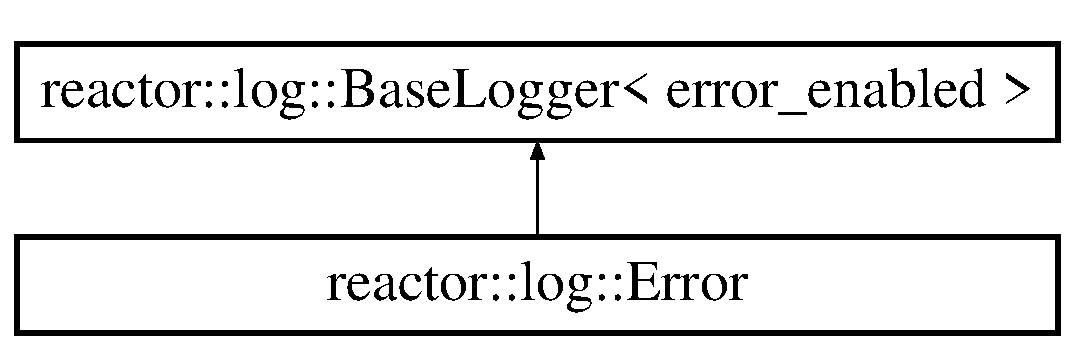
\includegraphics[height=2.000000cm]{structreactor_1_1log_1_1Error}
\end{center}
\end{figure}
\subsection*{Public Member Functions}
\begin{DoxyCompactItemize}
\item 
\hyperlink{structreactor_1_1log_1_1Error_adf478efdd9543d086e970afd9d63de04}{Error} ()
\end{DoxyCompactItemize}


\subsection{Constructor \& Destructor Documentation}
\mbox{\Hypertarget{structreactor_1_1log_1_1Error_adf478efdd9543d086e970afd9d63de04}\label{structreactor_1_1log_1_1Error_adf478efdd9543d086e970afd9d63de04}} 
\index{reactor\+::log\+::\+Error@{reactor\+::log\+::\+Error}!Error@{Error}}
\index{Error@{Error}!reactor\+::log\+::\+Error@{reactor\+::log\+::\+Error}}
\subsubsection{\texorpdfstring{Error()}{Error()}}
{\footnotesize\ttfamily reactor\+::log\+::\+Error\+::\+Error (\begin{DoxyParamCaption}{ }\end{DoxyParamCaption})\hspace{0.3cm}{\ttfamily [inline]}}



The documentation for this struct was generated from the following file\+:\begin{DoxyCompactItemize}
\item 
/home/runner/work/reactor-\/cpp/reactor-\/cpp/include/reactor-\/cpp/\hyperlink{logging_8hh}{logging.\+hh}\end{DoxyCompactItemize}

\hypertarget{classreactor_1_1ImmutableValuePtr}{}\section{reactor\+:\+:Immutable\+Value\+Ptr$<$ T $>$ Class Template Reference}
\label{classreactor_1_1ImmutableValuePtr}\index{reactor\+::\+Immutable\+Value\+Ptr$<$ T $>$@{reactor\+::\+Immutable\+Value\+Ptr$<$ T $>$}}


{\ttfamily \#include $<$value\+\_\+ptr.\+hh$>$}

\subsection*{Public Types}
\begin{DoxyCompactItemize}
\item 
using \hyperlink{classreactor_1_1ImmutableValuePtr_a88dbe82ff9b732b87e054ee37254bdfa}{type} = T
\end{DoxyCompactItemize}
\subsection*{Public Member Functions}
\begin{DoxyCompactItemize}
\item 
constexpr \hyperlink{classreactor_1_1ImmutableValuePtr_aa7bbdefa52d839dbf71a1b8369754356}{Immutable\+Value\+Ptr} ()
\item 
\hyperlink{classreactor_1_1ImmutableValuePtr_a607b854e71fd1ec5333ae97b15b8fc8d}{Immutable\+Value\+Ptr} (const \hyperlink{classreactor_1_1ImmutableValuePtr}{Immutable\+Value\+Ptr} \&)=default
\item 
\hyperlink{classreactor_1_1ImmutableValuePtr_acd518265a1c01dd99d48254922264f23}{Immutable\+Value\+Ptr} (\hyperlink{classreactor_1_1ImmutableValuePtr}{Immutable\+Value\+Ptr} \&\&)=default
\item 
constexpr \hyperlink{classreactor_1_1ImmutableValuePtr_aec3f1f481dc495293453c32f8654b5bc}{Immutable\+Value\+Ptr} (std\+::nullptr\+\_\+t)
\item 
\hyperlink{classreactor_1_1ImmutableValuePtr_a7b1b937ccd6dd4875c3737ba2780019f}{Immutable\+Value\+Ptr} (\hyperlink{classreactor_1_1MutableValuePtr}{Mutable\+Value\+Ptr}$<$ T $>$ \&\&ptr)
\item 
\hyperlink{classreactor_1_1ImmutableValuePtr}{Immutable\+Value\+Ptr} \& \hyperlink{classreactor_1_1ImmutableValuePtr_a94521923de3774c88536498461c5fd6b}{operator=} (std\+::nullptr\+\_\+t)
\item 
\hyperlink{classreactor_1_1ImmutableValuePtr}{Immutable\+Value\+Ptr} \& \hyperlink{classreactor_1_1ImmutableValuePtr_a0cf1105a09d40db7ceae985f9b329a9f}{operator=} (const \hyperlink{classreactor_1_1ImmutableValuePtr}{Immutable\+Value\+Ptr} \&ptr)
\item 
\hyperlink{classreactor_1_1ImmutableValuePtr}{Immutable\+Value\+Ptr} \& \hyperlink{classreactor_1_1ImmutableValuePtr_adeb3de5c3f0dc27613a4b3915f9747e7}{operator=} (\hyperlink{classreactor_1_1ImmutableValuePtr}{Immutable\+Value\+Ptr} \&\&ptr)
\item 
\hyperlink{classreactor_1_1ImmutableValuePtr_a88dbe82ff9b732b87e054ee37254bdfa}{type} $\ast$ \hyperlink{classreactor_1_1ImmutableValuePtr_a65630b7319b433ce022e660866bc27d1}{get} () const
\item 
\hyperlink{classreactor_1_1ImmutableValuePtr_a214067c64b236305411402aa0f332228}{operator bool} () const
\item 
\hyperlink{classreactor_1_1ImmutableValuePtr_a88dbe82ff9b732b87e054ee37254bdfa}{type} \& \hyperlink{classreactor_1_1ImmutableValuePtr_a1cbbf368f886f35c63604424f9b3b393}{operator$\ast$} () const
\item 
\hyperlink{classreactor_1_1ImmutableValuePtr_a88dbe82ff9b732b87e054ee37254bdfa}{type} $\ast$ \hyperlink{classreactor_1_1ImmutableValuePtr_af547b7a43033f0fbe383665c10335173}{operator-\/$>$} () const
\item 
\hyperlink{classreactor_1_1MutableValuePtr}{Mutable\+Value\+Ptr}$<$ T $>$ \hyperlink{classreactor_1_1ImmutableValuePtr_a642520ceaad885335b2e03e319c59749}{get\+\_\+mutable\+\_\+copy} () const
\end{DoxyCompactItemize}
\subsection*{Private Member Functions}
\begin{DoxyCompactItemize}
\item 
\hyperlink{classreactor_1_1ImmutableValuePtr_ae0d6edc13d77e9a68811d200c02fef84}{Immutable\+Value\+Ptr} (\hyperlink{classreactor_1_1ImmutableValuePtr_a88dbe82ff9b732b87e054ee37254bdfa}{type} $\ast$ptr)
\end{DoxyCompactItemize}
\subsection*{Private Attributes}
\begin{DoxyCompactItemize}
\item 
std\+::shared\+\_\+ptr$<$ \hyperlink{classreactor_1_1ImmutableValuePtr_a88dbe82ff9b732b87e054ee37254bdfa}{type} $>$ \hyperlink{classreactor_1_1ImmutableValuePtr_afe0edfdeed222658f79ce58dc2d8a0d6}{internal\+\_\+ptr}
\end{DoxyCompactItemize}
\subsection*{Friends}
\begin{DoxyCompactItemize}
\item 
{\footnotesize template$<$class U , class... Args$>$ }\\\hyperlink{classreactor_1_1ImmutableValuePtr}{Immutable\+Value\+Ptr}$<$ U $>$ \hyperlink{classreactor_1_1ImmutableValuePtr_a9fe212a2e336629d1f6df1b337f58c3f}{make\+\_\+immutable\+\_\+value} (Args \&\&... args)
\end{DoxyCompactItemize}


\subsection{Member Typedef Documentation}
\mbox{\Hypertarget{classreactor_1_1ImmutableValuePtr_a88dbe82ff9b732b87e054ee37254bdfa}\label{classreactor_1_1ImmutableValuePtr_a88dbe82ff9b732b87e054ee37254bdfa}} 
\index{reactor\+::\+Immutable\+Value\+Ptr@{reactor\+::\+Immutable\+Value\+Ptr}!type@{type}}
\index{type@{type}!reactor\+::\+Immutable\+Value\+Ptr@{reactor\+::\+Immutable\+Value\+Ptr}}
\subsubsection{\texorpdfstring{type}{type}}
{\footnotesize\ttfamily template$<$class T$>$ \\
using \hyperlink{classreactor_1_1ImmutableValuePtr}{reactor\+::\+Immutable\+Value\+Ptr}$<$ T $>$\+::\hyperlink{classreactor_1_1ImmutableValuePtr_a88dbe82ff9b732b87e054ee37254bdfa}{type} =  T}



\subsection{Constructor \& Destructor Documentation}
\mbox{\Hypertarget{classreactor_1_1ImmutableValuePtr_ae0d6edc13d77e9a68811d200c02fef84}\label{classreactor_1_1ImmutableValuePtr_ae0d6edc13d77e9a68811d200c02fef84}} 
\index{reactor\+::\+Immutable\+Value\+Ptr@{reactor\+::\+Immutable\+Value\+Ptr}!Immutable\+Value\+Ptr@{Immutable\+Value\+Ptr}}
\index{Immutable\+Value\+Ptr@{Immutable\+Value\+Ptr}!reactor\+::\+Immutable\+Value\+Ptr@{reactor\+::\+Immutable\+Value\+Ptr}}
\subsubsection{\texorpdfstring{Immutable\+Value\+Ptr()}{ImmutableValuePtr()}\hspace{0.1cm}{\footnotesize\ttfamily [1/6]}}
{\footnotesize\ttfamily template$<$class T$>$ \\
\hyperlink{classreactor_1_1ImmutableValuePtr}{reactor\+::\+Immutable\+Value\+Ptr}$<$ T $>$\+::\hyperlink{classreactor_1_1ImmutableValuePtr}{Immutable\+Value\+Ptr} (\begin{DoxyParamCaption}\item[{\hyperlink{classreactor_1_1ImmutableValuePtr_a88dbe82ff9b732b87e054ee37254bdfa}{type} $\ast$}]{ptr }\end{DoxyParamCaption})\hspace{0.3cm}{\ttfamily [inline]}, {\ttfamily [explicit]}, {\ttfamily [private]}}

\mbox{\Hypertarget{classreactor_1_1ImmutableValuePtr_aa7bbdefa52d839dbf71a1b8369754356}\label{classreactor_1_1ImmutableValuePtr_aa7bbdefa52d839dbf71a1b8369754356}} 
\index{reactor\+::\+Immutable\+Value\+Ptr@{reactor\+::\+Immutable\+Value\+Ptr}!Immutable\+Value\+Ptr@{Immutable\+Value\+Ptr}}
\index{Immutable\+Value\+Ptr@{Immutable\+Value\+Ptr}!reactor\+::\+Immutable\+Value\+Ptr@{reactor\+::\+Immutable\+Value\+Ptr}}
\subsubsection{\texorpdfstring{Immutable\+Value\+Ptr()}{ImmutableValuePtr()}\hspace{0.1cm}{\footnotesize\ttfamily [2/6]}}
{\footnotesize\ttfamily template$<$class T$>$ \\
constexpr \hyperlink{classreactor_1_1ImmutableValuePtr}{reactor\+::\+Immutable\+Value\+Ptr}$<$ T $>$\+::\hyperlink{classreactor_1_1ImmutableValuePtr}{Immutable\+Value\+Ptr} (\begin{DoxyParamCaption}{ }\end{DoxyParamCaption})\hspace{0.3cm}{\ttfamily [inline]}}

\mbox{\Hypertarget{classreactor_1_1ImmutableValuePtr_a607b854e71fd1ec5333ae97b15b8fc8d}\label{classreactor_1_1ImmutableValuePtr_a607b854e71fd1ec5333ae97b15b8fc8d}} 
\index{reactor\+::\+Immutable\+Value\+Ptr@{reactor\+::\+Immutable\+Value\+Ptr}!Immutable\+Value\+Ptr@{Immutable\+Value\+Ptr}}
\index{Immutable\+Value\+Ptr@{Immutable\+Value\+Ptr}!reactor\+::\+Immutable\+Value\+Ptr@{reactor\+::\+Immutable\+Value\+Ptr}}
\subsubsection{\texorpdfstring{Immutable\+Value\+Ptr()}{ImmutableValuePtr()}\hspace{0.1cm}{\footnotesize\ttfamily [3/6]}}
{\footnotesize\ttfamily template$<$class T$>$ \\
\hyperlink{classreactor_1_1ImmutableValuePtr}{reactor\+::\+Immutable\+Value\+Ptr}$<$ T $>$\+::\hyperlink{classreactor_1_1ImmutableValuePtr}{Immutable\+Value\+Ptr} (\begin{DoxyParamCaption}\item[{const \hyperlink{classreactor_1_1ImmutableValuePtr}{Immutable\+Value\+Ptr}$<$ T $>$ \&}]{ }\end{DoxyParamCaption})\hspace{0.3cm}{\ttfamily [default]}}

\mbox{\Hypertarget{classreactor_1_1ImmutableValuePtr_acd518265a1c01dd99d48254922264f23}\label{classreactor_1_1ImmutableValuePtr_acd518265a1c01dd99d48254922264f23}} 
\index{reactor\+::\+Immutable\+Value\+Ptr@{reactor\+::\+Immutable\+Value\+Ptr}!Immutable\+Value\+Ptr@{Immutable\+Value\+Ptr}}
\index{Immutable\+Value\+Ptr@{Immutable\+Value\+Ptr}!reactor\+::\+Immutable\+Value\+Ptr@{reactor\+::\+Immutable\+Value\+Ptr}}
\subsubsection{\texorpdfstring{Immutable\+Value\+Ptr()}{ImmutableValuePtr()}\hspace{0.1cm}{\footnotesize\ttfamily [4/6]}}
{\footnotesize\ttfamily template$<$class T$>$ \\
\hyperlink{classreactor_1_1ImmutableValuePtr}{reactor\+::\+Immutable\+Value\+Ptr}$<$ T $>$\+::\hyperlink{classreactor_1_1ImmutableValuePtr}{Immutable\+Value\+Ptr} (\begin{DoxyParamCaption}\item[{\hyperlink{classreactor_1_1ImmutableValuePtr}{Immutable\+Value\+Ptr}$<$ T $>$ \&\&}]{ }\end{DoxyParamCaption})\hspace{0.3cm}{\ttfamily [default]}}

\mbox{\Hypertarget{classreactor_1_1ImmutableValuePtr_aec3f1f481dc495293453c32f8654b5bc}\label{classreactor_1_1ImmutableValuePtr_aec3f1f481dc495293453c32f8654b5bc}} 
\index{reactor\+::\+Immutable\+Value\+Ptr@{reactor\+::\+Immutable\+Value\+Ptr}!Immutable\+Value\+Ptr@{Immutable\+Value\+Ptr}}
\index{Immutable\+Value\+Ptr@{Immutable\+Value\+Ptr}!reactor\+::\+Immutable\+Value\+Ptr@{reactor\+::\+Immutable\+Value\+Ptr}}
\subsubsection{\texorpdfstring{Immutable\+Value\+Ptr()}{ImmutableValuePtr()}\hspace{0.1cm}{\footnotesize\ttfamily [5/6]}}
{\footnotesize\ttfamily template$<$class T$>$ \\
constexpr \hyperlink{classreactor_1_1ImmutableValuePtr}{reactor\+::\+Immutable\+Value\+Ptr}$<$ T $>$\+::\hyperlink{classreactor_1_1ImmutableValuePtr}{Immutable\+Value\+Ptr} (\begin{DoxyParamCaption}\item[{std\+::nullptr\+\_\+t}]{ }\end{DoxyParamCaption})\hspace{0.3cm}{\ttfamily [inline]}, {\ttfamily [explicit]}}

\mbox{\Hypertarget{classreactor_1_1ImmutableValuePtr_a7b1b937ccd6dd4875c3737ba2780019f}\label{classreactor_1_1ImmutableValuePtr_a7b1b937ccd6dd4875c3737ba2780019f}} 
\index{reactor\+::\+Immutable\+Value\+Ptr@{reactor\+::\+Immutable\+Value\+Ptr}!Immutable\+Value\+Ptr@{Immutable\+Value\+Ptr}}
\index{Immutable\+Value\+Ptr@{Immutable\+Value\+Ptr}!reactor\+::\+Immutable\+Value\+Ptr@{reactor\+::\+Immutable\+Value\+Ptr}}
\subsubsection{\texorpdfstring{Immutable\+Value\+Ptr()}{ImmutableValuePtr()}\hspace{0.1cm}{\footnotesize\ttfamily [6/6]}}
{\footnotesize\ttfamily template$<$class T$>$ \\
\hyperlink{classreactor_1_1ImmutableValuePtr}{reactor\+::\+Immutable\+Value\+Ptr}$<$ T $>$\+::\hyperlink{classreactor_1_1ImmutableValuePtr}{Immutable\+Value\+Ptr} (\begin{DoxyParamCaption}\item[{\hyperlink{classreactor_1_1MutableValuePtr}{Mutable\+Value\+Ptr}$<$ T $>$ \&\&}]{ptr }\end{DoxyParamCaption})\hspace{0.3cm}{\ttfamily [inline]}, {\ttfamily [explicit]}}



\subsection{Member Function Documentation}
\mbox{\Hypertarget{classreactor_1_1ImmutableValuePtr_a65630b7319b433ce022e660866bc27d1}\label{classreactor_1_1ImmutableValuePtr_a65630b7319b433ce022e660866bc27d1}} 
\index{reactor\+::\+Immutable\+Value\+Ptr@{reactor\+::\+Immutable\+Value\+Ptr}!get@{get}}
\index{get@{get}!reactor\+::\+Immutable\+Value\+Ptr@{reactor\+::\+Immutable\+Value\+Ptr}}
\subsubsection{\texorpdfstring{get()}{get()}}
{\footnotesize\ttfamily template$<$class T$>$ \\
\hyperlink{classreactor_1_1ImmutableValuePtr_a88dbe82ff9b732b87e054ee37254bdfa}{type}$\ast$ \hyperlink{classreactor_1_1ImmutableValuePtr}{reactor\+::\+Immutable\+Value\+Ptr}$<$ T $>$\+::get (\begin{DoxyParamCaption}{ }\end{DoxyParamCaption}) const\hspace{0.3cm}{\ttfamily [inline]}}

\mbox{\Hypertarget{classreactor_1_1ImmutableValuePtr_a642520ceaad885335b2e03e319c59749}\label{classreactor_1_1ImmutableValuePtr_a642520ceaad885335b2e03e319c59749}} 
\index{reactor\+::\+Immutable\+Value\+Ptr@{reactor\+::\+Immutable\+Value\+Ptr}!get\+\_\+mutable\+\_\+copy@{get\+\_\+mutable\+\_\+copy}}
\index{get\+\_\+mutable\+\_\+copy@{get\+\_\+mutable\+\_\+copy}!reactor\+::\+Immutable\+Value\+Ptr@{reactor\+::\+Immutable\+Value\+Ptr}}
\subsubsection{\texorpdfstring{get\+\_\+mutable\+\_\+copy()}{get\_mutable\_copy()}}
{\footnotesize\ttfamily template$<$class T$>$ \\
\hyperlink{classreactor_1_1MutableValuePtr}{Mutable\+Value\+Ptr}$<$T$>$ \hyperlink{classreactor_1_1ImmutableValuePtr}{reactor\+::\+Immutable\+Value\+Ptr}$<$ T $>$\+::get\+\_\+mutable\+\_\+copy (\begin{DoxyParamCaption}{ }\end{DoxyParamCaption}) const\hspace{0.3cm}{\ttfamily [inline]}}

\mbox{\Hypertarget{classreactor_1_1ImmutableValuePtr_a214067c64b236305411402aa0f332228}\label{classreactor_1_1ImmutableValuePtr_a214067c64b236305411402aa0f332228}} 
\index{reactor\+::\+Immutable\+Value\+Ptr@{reactor\+::\+Immutable\+Value\+Ptr}!operator bool@{operator bool}}
\index{operator bool@{operator bool}!reactor\+::\+Immutable\+Value\+Ptr@{reactor\+::\+Immutable\+Value\+Ptr}}
\subsubsection{\texorpdfstring{operator bool()}{operator bool()}}
{\footnotesize\ttfamily template$<$class T$>$ \\
\hyperlink{classreactor_1_1ImmutableValuePtr}{reactor\+::\+Immutable\+Value\+Ptr}$<$ T $>$\+::operator bool (\begin{DoxyParamCaption}{ }\end{DoxyParamCaption}) const\hspace{0.3cm}{\ttfamily [inline]}, {\ttfamily [explicit]}}

\mbox{\Hypertarget{classreactor_1_1ImmutableValuePtr_a1cbbf368f886f35c63604424f9b3b393}\label{classreactor_1_1ImmutableValuePtr_a1cbbf368f886f35c63604424f9b3b393}} 
\index{reactor\+::\+Immutable\+Value\+Ptr@{reactor\+::\+Immutable\+Value\+Ptr}!operator$\ast$@{operator$\ast$}}
\index{operator$\ast$@{operator$\ast$}!reactor\+::\+Immutable\+Value\+Ptr@{reactor\+::\+Immutable\+Value\+Ptr}}
\subsubsection{\texorpdfstring{operator$\ast$()}{operator*()}}
{\footnotesize\ttfamily template$<$class T$>$ \\
\hyperlink{classreactor_1_1ImmutableValuePtr_a88dbe82ff9b732b87e054ee37254bdfa}{type}\& \hyperlink{classreactor_1_1ImmutableValuePtr}{reactor\+::\+Immutable\+Value\+Ptr}$<$ T $>$\+::operator$\ast$ (\begin{DoxyParamCaption}{ }\end{DoxyParamCaption}) const\hspace{0.3cm}{\ttfamily [inline]}}

\mbox{\Hypertarget{classreactor_1_1ImmutableValuePtr_af547b7a43033f0fbe383665c10335173}\label{classreactor_1_1ImmutableValuePtr_af547b7a43033f0fbe383665c10335173}} 
\index{reactor\+::\+Immutable\+Value\+Ptr@{reactor\+::\+Immutable\+Value\+Ptr}!operator-\/$>$@{operator-\/$>$}}
\index{operator-\/$>$@{operator-\/$>$}!reactor\+::\+Immutable\+Value\+Ptr@{reactor\+::\+Immutable\+Value\+Ptr}}
\subsubsection{\texorpdfstring{operator-\/$>$()}{operator->()}}
{\footnotesize\ttfamily template$<$class T$>$ \\
\hyperlink{classreactor_1_1ImmutableValuePtr_a88dbe82ff9b732b87e054ee37254bdfa}{type}$\ast$ \hyperlink{classreactor_1_1ImmutableValuePtr}{reactor\+::\+Immutable\+Value\+Ptr}$<$ T $>$\+::operator-\/$>$ (\begin{DoxyParamCaption}{ }\end{DoxyParamCaption}) const\hspace{0.3cm}{\ttfamily [inline]}}

\mbox{\Hypertarget{classreactor_1_1ImmutableValuePtr_a94521923de3774c88536498461c5fd6b}\label{classreactor_1_1ImmutableValuePtr_a94521923de3774c88536498461c5fd6b}} 
\index{reactor\+::\+Immutable\+Value\+Ptr@{reactor\+::\+Immutable\+Value\+Ptr}!operator=@{operator=}}
\index{operator=@{operator=}!reactor\+::\+Immutable\+Value\+Ptr@{reactor\+::\+Immutable\+Value\+Ptr}}
\subsubsection{\texorpdfstring{operator=()}{operator=()}\hspace{0.1cm}{\footnotesize\ttfamily [1/3]}}
{\footnotesize\ttfamily template$<$class T$>$ \\
\hyperlink{classreactor_1_1ImmutableValuePtr}{Immutable\+Value\+Ptr}\& \hyperlink{classreactor_1_1ImmutableValuePtr}{reactor\+::\+Immutable\+Value\+Ptr}$<$ T $>$\+::operator= (\begin{DoxyParamCaption}\item[{std\+::nullptr\+\_\+t}]{ }\end{DoxyParamCaption})\hspace{0.3cm}{\ttfamily [inline]}}

\mbox{\Hypertarget{classreactor_1_1ImmutableValuePtr_a0cf1105a09d40db7ceae985f9b329a9f}\label{classreactor_1_1ImmutableValuePtr_a0cf1105a09d40db7ceae985f9b329a9f}} 
\index{reactor\+::\+Immutable\+Value\+Ptr@{reactor\+::\+Immutable\+Value\+Ptr}!operator=@{operator=}}
\index{operator=@{operator=}!reactor\+::\+Immutable\+Value\+Ptr@{reactor\+::\+Immutable\+Value\+Ptr}}
\subsubsection{\texorpdfstring{operator=()}{operator=()}\hspace{0.1cm}{\footnotesize\ttfamily [2/3]}}
{\footnotesize\ttfamily template$<$class T$>$ \\
\hyperlink{classreactor_1_1ImmutableValuePtr}{Immutable\+Value\+Ptr}\& \hyperlink{classreactor_1_1ImmutableValuePtr}{reactor\+::\+Immutable\+Value\+Ptr}$<$ T $>$\+::operator= (\begin{DoxyParamCaption}\item[{const \hyperlink{classreactor_1_1ImmutableValuePtr}{Immutable\+Value\+Ptr}$<$ T $>$ \&}]{ptr }\end{DoxyParamCaption})\hspace{0.3cm}{\ttfamily [inline]}}

\mbox{\Hypertarget{classreactor_1_1ImmutableValuePtr_adeb3de5c3f0dc27613a4b3915f9747e7}\label{classreactor_1_1ImmutableValuePtr_adeb3de5c3f0dc27613a4b3915f9747e7}} 
\index{reactor\+::\+Immutable\+Value\+Ptr@{reactor\+::\+Immutable\+Value\+Ptr}!operator=@{operator=}}
\index{operator=@{operator=}!reactor\+::\+Immutable\+Value\+Ptr@{reactor\+::\+Immutable\+Value\+Ptr}}
\subsubsection{\texorpdfstring{operator=()}{operator=()}\hspace{0.1cm}{\footnotesize\ttfamily [3/3]}}
{\footnotesize\ttfamily template$<$class T$>$ \\
\hyperlink{classreactor_1_1ImmutableValuePtr}{Immutable\+Value\+Ptr}\& \hyperlink{classreactor_1_1ImmutableValuePtr}{reactor\+::\+Immutable\+Value\+Ptr}$<$ T $>$\+::operator= (\begin{DoxyParamCaption}\item[{\hyperlink{classreactor_1_1ImmutableValuePtr}{Immutable\+Value\+Ptr}$<$ T $>$ \&\&}]{ptr }\end{DoxyParamCaption})\hspace{0.3cm}{\ttfamily [inline]}}



\subsection{Friends And Related Function Documentation}
\mbox{\Hypertarget{classreactor_1_1ImmutableValuePtr_a9fe212a2e336629d1f6df1b337f58c3f}\label{classreactor_1_1ImmutableValuePtr_a9fe212a2e336629d1f6df1b337f58c3f}} 
\index{reactor\+::\+Immutable\+Value\+Ptr@{reactor\+::\+Immutable\+Value\+Ptr}!make\+\_\+immutable\+\_\+value@{make\+\_\+immutable\+\_\+value}}
\index{make\+\_\+immutable\+\_\+value@{make\+\_\+immutable\+\_\+value}!reactor\+::\+Immutable\+Value\+Ptr@{reactor\+::\+Immutable\+Value\+Ptr}}
\subsubsection{\texorpdfstring{make\+\_\+immutable\+\_\+value}{make\_immutable\_value}}
{\footnotesize\ttfamily template$<$class T$>$ \\
template$<$class U , class... Args$>$ \\
\hyperlink{classreactor_1_1ImmutableValuePtr}{Immutable\+Value\+Ptr}$<$U$>$ make\+\_\+immutable\+\_\+value (\begin{DoxyParamCaption}\item[{Args \&\&...}]{args }\end{DoxyParamCaption})\hspace{0.3cm}{\ttfamily [friend]}}



\subsection{Member Data Documentation}
\mbox{\Hypertarget{classreactor_1_1ImmutableValuePtr_afe0edfdeed222658f79ce58dc2d8a0d6}\label{classreactor_1_1ImmutableValuePtr_afe0edfdeed222658f79ce58dc2d8a0d6}} 
\index{reactor\+::\+Immutable\+Value\+Ptr@{reactor\+::\+Immutable\+Value\+Ptr}!internal\+\_\+ptr@{internal\+\_\+ptr}}
\index{internal\+\_\+ptr@{internal\+\_\+ptr}!reactor\+::\+Immutable\+Value\+Ptr@{reactor\+::\+Immutable\+Value\+Ptr}}
\subsubsection{\texorpdfstring{internal\+\_\+ptr}{internal\_ptr}}
{\footnotesize\ttfamily template$<$class T$>$ \\
std\+::shared\+\_\+ptr$<$\hyperlink{classreactor_1_1ImmutableValuePtr_a88dbe82ff9b732b87e054ee37254bdfa}{type}$>$ \hyperlink{classreactor_1_1ImmutableValuePtr}{reactor\+::\+Immutable\+Value\+Ptr}$<$ T $>$\+::internal\+\_\+ptr\hspace{0.3cm}{\ttfamily [private]}}



The documentation for this class was generated from the following file\+:\begin{DoxyCompactItemize}
\item 
/home/runner/work/reactor-\/cpp/reactor-\/cpp/include/reactor-\/cpp/\hyperlink{value__ptr_8hh}{value\+\_\+ptr.\+hh}\end{DoxyCompactItemize}

\hypertarget{structreactor_1_1log_1_1Info}{}\section{reactor\+:\+:log\+:\+:Info Struct Reference}
\label{structreactor_1_1log_1_1Info}\index{reactor\+::log\+::\+Info@{reactor\+::log\+::\+Info}}


{\ttfamily \#include $<$logging.\+hh$>$}

Inheritance diagram for reactor\+:\+:log\+:\+:Info\+:\begin{figure}[H]
\begin{center}
\leavevmode
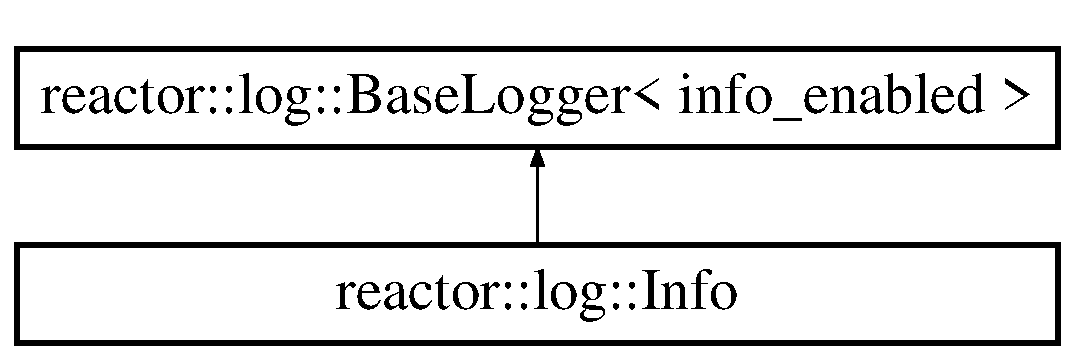
\includegraphics[height=2.000000cm]{structreactor_1_1log_1_1Info}
\end{center}
\end{figure}
\subsection*{Public Member Functions}
\begin{DoxyCompactItemize}
\item 
\hyperlink{structreactor_1_1log_1_1Info_abad3878de5e3c6e752d926c78e7da194}{Info} ()
\end{DoxyCompactItemize}


\subsection{Constructor \& Destructor Documentation}
\mbox{\Hypertarget{structreactor_1_1log_1_1Info_abad3878de5e3c6e752d926c78e7da194}\label{structreactor_1_1log_1_1Info_abad3878de5e3c6e752d926c78e7da194}} 
\index{reactor\+::log\+::\+Info@{reactor\+::log\+::\+Info}!Info@{Info}}
\index{Info@{Info}!reactor\+::log\+::\+Info@{reactor\+::log\+::\+Info}}
\subsubsection{\texorpdfstring{Info()}{Info()}}
{\footnotesize\ttfamily reactor\+::log\+::\+Info\+::\+Info (\begin{DoxyParamCaption}{ }\end{DoxyParamCaption})\hspace{0.3cm}{\ttfamily [inline]}}



The documentation for this struct was generated from the following file\+:\begin{DoxyCompactItemize}
\item 
/home/runner/work/reactor-\/cpp/reactor-\/cpp/include/reactor-\/cpp/\hyperlink{logging_8hh}{logging.\+hh}\end{DoxyCompactItemize}

\hypertarget{classreactor_1_1Input}{}\section{reactor\+:\+:Input$<$ T $>$ Class Template Reference}
\label{classreactor_1_1Input}\index{reactor\+::\+Input$<$ T $>$@{reactor\+::\+Input$<$ T $>$}}


{\ttfamily \#include $<$port.\+hh$>$}

Inheritance diagram for reactor\+:\+:Input$<$ T $>$\+:\begin{figure}[H]
\begin{center}
\leavevmode
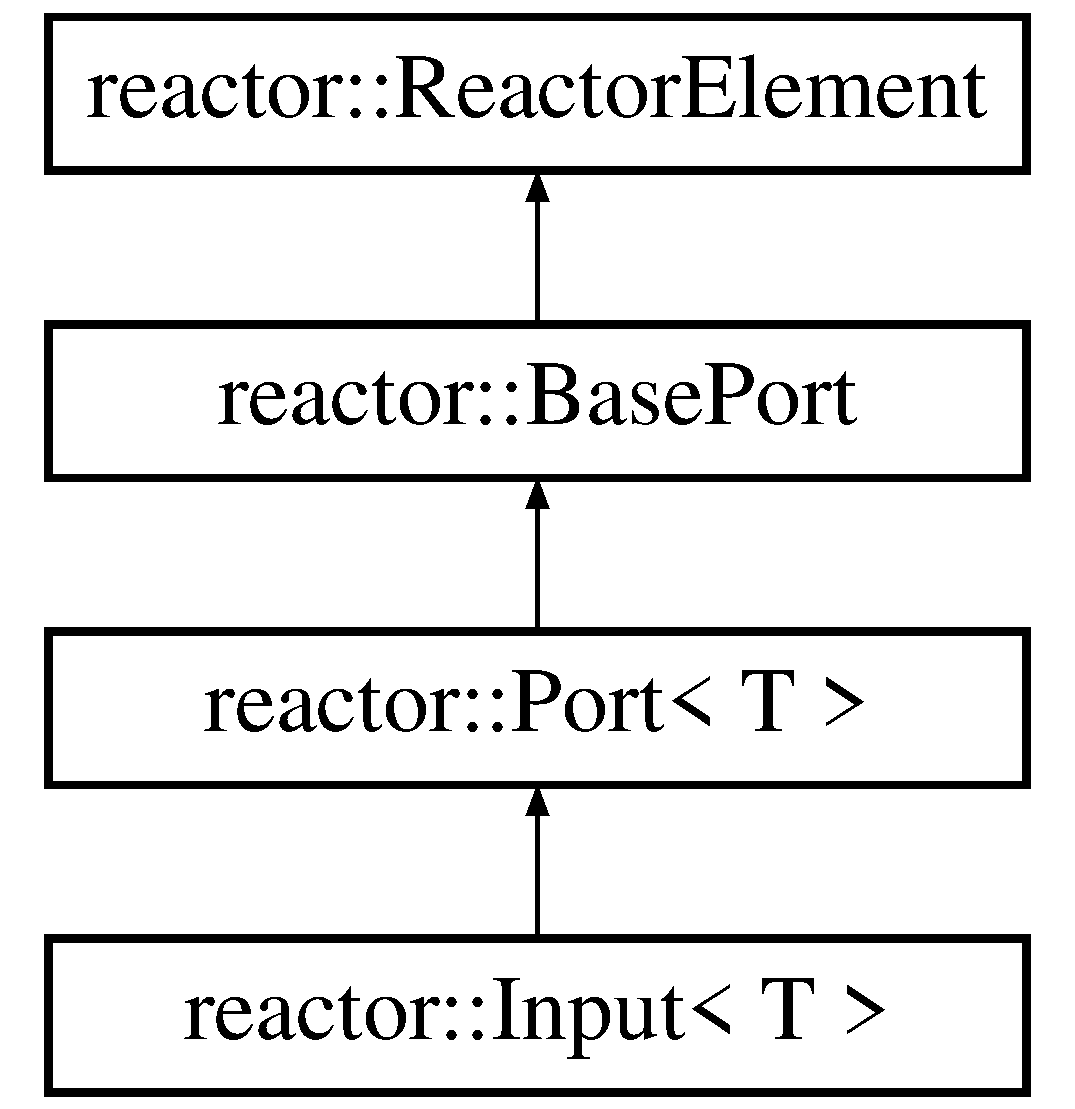
\includegraphics[height=4.000000cm]{classreactor_1_1Input}
\end{center}
\end{figure}
\subsection*{Public Member Functions}
\begin{DoxyCompactItemize}
\item 
\hyperlink{classreactor_1_1Input_a1c035f6840e363d515d92a4a20cd3b6a}{Input} (const std\+::string \&\hyperlink{classreactor_1_1ReactorElement_a99579f61dbaf5d5d98aebfe26eb8bf77}{name}, \hyperlink{classreactor_1_1Reactor}{Reactor} $\ast$\hyperlink{classreactor_1_1ReactorElement_a25bf298de879a82eefc1ba426be05812}{container})
\end{DoxyCompactItemize}
\subsection*{Additional Inherited Members}


\subsection{Constructor \& Destructor Documentation}
\mbox{\Hypertarget{classreactor_1_1Input_a1c035f6840e363d515d92a4a20cd3b6a}\label{classreactor_1_1Input_a1c035f6840e363d515d92a4a20cd3b6a}} 
\index{reactor\+::\+Input@{reactor\+::\+Input}!Input@{Input}}
\index{Input@{Input}!reactor\+::\+Input@{reactor\+::\+Input}}
\subsubsection{\texorpdfstring{Input()}{Input()}}
{\footnotesize\ttfamily template$<$class T $>$ \\
\hyperlink{classreactor_1_1Input}{reactor\+::\+Input}$<$ T $>$\+::\hyperlink{classreactor_1_1Input}{Input} (\begin{DoxyParamCaption}\item[{const std\+::string \&}]{name,  }\item[{\hyperlink{classreactor_1_1Reactor}{Reactor} $\ast$}]{container }\end{DoxyParamCaption})\hspace{0.3cm}{\ttfamily [inline]}}



The documentation for this class was generated from the following file\+:\begin{DoxyCompactItemize}
\item 
/home/runner/work/reactor-\/cpp/reactor-\/cpp/include/reactor-\/cpp/\hyperlink{port_8hh}{port.\+hh}\end{DoxyCompactItemize}

\hypertarget{classreactor_1_1LogicalAction}{}\section{reactor\+:\+:Logical\+Action$<$ T $>$ Class Template Reference}
\label{classreactor_1_1LogicalAction}\index{reactor\+::\+Logical\+Action$<$ T $>$@{reactor\+::\+Logical\+Action$<$ T $>$}}


{\ttfamily \#include $<$action.\+hh$>$}

Inheritance diagram for reactor\+:\+:Logical\+Action$<$ T $>$\+:\begin{figure}[H]
\begin{center}
\leavevmode
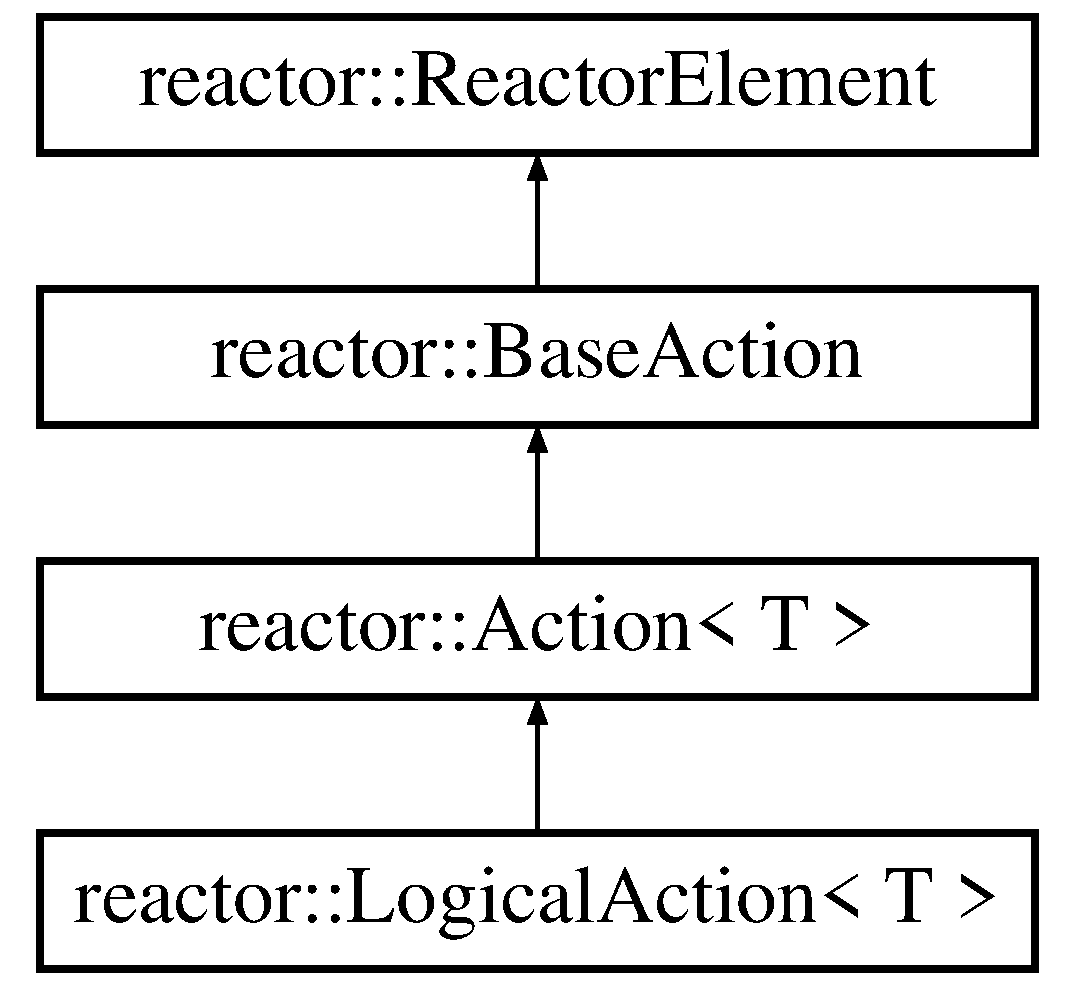
\includegraphics[height=4.000000cm]{classreactor_1_1LogicalAction}
\end{center}
\end{figure}
\subsection*{Public Member Functions}
\begin{DoxyCompactItemize}
\item 
\hyperlink{classreactor_1_1LogicalAction_abb4c5b2637a33f13be3aa182758bb510}{Logical\+Action} (const std\+::string \&\hyperlink{classreactor_1_1ReactorElement_a99579f61dbaf5d5d98aebfe26eb8bf77}{name}, \hyperlink{classreactor_1_1Reactor}{Reactor} $\ast$\hyperlink{classreactor_1_1ReactorElement_a25bf298de879a82eefc1ba426be05812}{container}, \hyperlink{namespacereactor_aa8375b807a80703545664096c5b5b779}{Duration} \hyperlink{classreactor_1_1BaseAction_a98201db474f34cb9e38151a6960128f0}{min\+\_\+delay}=Duration\+::zero())
\end{DoxyCompactItemize}
\subsection*{Additional Inherited Members}


\subsection{Constructor \& Destructor Documentation}
\mbox{\Hypertarget{classreactor_1_1LogicalAction_abb4c5b2637a33f13be3aa182758bb510}\label{classreactor_1_1LogicalAction_abb4c5b2637a33f13be3aa182758bb510}} 
\index{reactor\+::\+Logical\+Action@{reactor\+::\+Logical\+Action}!Logical\+Action@{Logical\+Action}}
\index{Logical\+Action@{Logical\+Action}!reactor\+::\+Logical\+Action@{reactor\+::\+Logical\+Action}}
\subsubsection{\texorpdfstring{Logical\+Action()}{LogicalAction()}}
{\footnotesize\ttfamily template$<$class T $>$ \\
\hyperlink{classreactor_1_1LogicalAction}{reactor\+::\+Logical\+Action}$<$ T $>$\+::\hyperlink{classreactor_1_1LogicalAction}{Logical\+Action} (\begin{DoxyParamCaption}\item[{const std\+::string \&}]{name,  }\item[{\hyperlink{classreactor_1_1Reactor}{Reactor} $\ast$}]{container,  }\item[{\hyperlink{namespacereactor_aa8375b807a80703545664096c5b5b779}{Duration}}]{min\+\_\+delay = {\ttfamily Duration\+:\+:zero()} }\end{DoxyParamCaption})\hspace{0.3cm}{\ttfamily [inline]}}



The documentation for this class was generated from the following file\+:\begin{DoxyCompactItemize}
\item 
/home/runner/work/reactor-\/cpp/reactor-\/cpp/include/reactor-\/cpp/\hyperlink{action_8hh}{action.\+hh}\end{DoxyCompactItemize}

\hypertarget{classreactor_1_1LogicalTime}{}\section{reactor\+:\+:Logical\+Time Class Reference}
\label{classreactor_1_1LogicalTime}\index{reactor\+::\+Logical\+Time@{reactor\+::\+Logical\+Time}}


{\ttfamily \#include $<$logical\+\_\+time.\+hh$>$}

\subsection*{Public Member Functions}
\begin{DoxyCompactItemize}
\item 
void \hyperlink{classreactor_1_1LogicalTime_a50fa399e89e28bece4a1198efe626110}{advance\+\_\+to} (const \hyperlink{classreactor_1_1Tag}{Tag} \&tag)
\item 
const \hyperlink{namespacereactor_ad950f8d1a46612500286a4af0f167080}{Time\+Point} \& \hyperlink{classreactor_1_1LogicalTime_a94567626de1241161edfb41c34d6b09e}{time\+\_\+point} () const
\item 
const \hyperlink{namespacereactor_aaea1189d617982457b74127ba74a7340}{mstep\+\_\+t} \& \hyperlink{classreactor_1_1LogicalTime_a59d2ded3742c8bcec0d9af22a45bd133}{micro\+\_\+step} () const
\end{DoxyCompactItemize}
\subsection*{Private Attributes}
\begin{DoxyCompactItemize}
\item 
\hyperlink{namespacereactor_ad950f8d1a46612500286a4af0f167080}{Time\+Point} \hyperlink{classreactor_1_1LogicalTime_a00ea2389e8dd656986c559690343d963}{\+\_\+time\+\_\+point} \{\}
\item 
\hyperlink{namespacereactor_aaea1189d617982457b74127ba74a7340}{mstep\+\_\+t} \hyperlink{classreactor_1_1LogicalTime_a54b9d7e8cd2af3523b92efbbac1969e9}{\+\_\+micro\+\_\+step} \{0\}
\end{DoxyCompactItemize}


\subsection{Member Function Documentation}
\mbox{\Hypertarget{classreactor_1_1LogicalTime_a50fa399e89e28bece4a1198efe626110}\label{classreactor_1_1LogicalTime_a50fa399e89e28bece4a1198efe626110}} 
\index{reactor\+::\+Logical\+Time@{reactor\+::\+Logical\+Time}!advance\+\_\+to@{advance\+\_\+to}}
\index{advance\+\_\+to@{advance\+\_\+to}!reactor\+::\+Logical\+Time@{reactor\+::\+Logical\+Time}}
\subsubsection{\texorpdfstring{advance\+\_\+to()}{advance\_to()}}
{\footnotesize\ttfamily void reactor\+::\+Logical\+Time\+::advance\+\_\+to (\begin{DoxyParamCaption}\item[{const \hyperlink{classreactor_1_1Tag}{Tag} \&}]{tag }\end{DoxyParamCaption})}

\mbox{\Hypertarget{classreactor_1_1LogicalTime_a59d2ded3742c8bcec0d9af22a45bd133}\label{classreactor_1_1LogicalTime_a59d2ded3742c8bcec0d9af22a45bd133}} 
\index{reactor\+::\+Logical\+Time@{reactor\+::\+Logical\+Time}!micro\+\_\+step@{micro\+\_\+step}}
\index{micro\+\_\+step@{micro\+\_\+step}!reactor\+::\+Logical\+Time@{reactor\+::\+Logical\+Time}}
\subsubsection{\texorpdfstring{micro\+\_\+step()}{micro\_step()}}
{\footnotesize\ttfamily const \hyperlink{namespacereactor_aaea1189d617982457b74127ba74a7340}{mstep\+\_\+t}\& reactor\+::\+Logical\+Time\+::micro\+\_\+step (\begin{DoxyParamCaption}{ }\end{DoxyParamCaption}) const\hspace{0.3cm}{\ttfamily [inline]}}

\mbox{\Hypertarget{classreactor_1_1LogicalTime_a94567626de1241161edfb41c34d6b09e}\label{classreactor_1_1LogicalTime_a94567626de1241161edfb41c34d6b09e}} 
\index{reactor\+::\+Logical\+Time@{reactor\+::\+Logical\+Time}!time\+\_\+point@{time\+\_\+point}}
\index{time\+\_\+point@{time\+\_\+point}!reactor\+::\+Logical\+Time@{reactor\+::\+Logical\+Time}}
\subsubsection{\texorpdfstring{time\+\_\+point()}{time\_point()}}
{\footnotesize\ttfamily const \hyperlink{namespacereactor_ad950f8d1a46612500286a4af0f167080}{Time\+Point}\& reactor\+::\+Logical\+Time\+::time\+\_\+point (\begin{DoxyParamCaption}{ }\end{DoxyParamCaption}) const\hspace{0.3cm}{\ttfamily [inline]}}



\subsection{Member Data Documentation}
\mbox{\Hypertarget{classreactor_1_1LogicalTime_a54b9d7e8cd2af3523b92efbbac1969e9}\label{classreactor_1_1LogicalTime_a54b9d7e8cd2af3523b92efbbac1969e9}} 
\index{reactor\+::\+Logical\+Time@{reactor\+::\+Logical\+Time}!\+\_\+micro\+\_\+step@{\+\_\+micro\+\_\+step}}
\index{\+\_\+micro\+\_\+step@{\+\_\+micro\+\_\+step}!reactor\+::\+Logical\+Time@{reactor\+::\+Logical\+Time}}
\subsubsection{\texorpdfstring{\+\_\+micro\+\_\+step}{\_micro\_step}}
{\footnotesize\ttfamily \hyperlink{namespacereactor_aaea1189d617982457b74127ba74a7340}{mstep\+\_\+t} reactor\+::\+Logical\+Time\+::\+\_\+micro\+\_\+step \{0\}\hspace{0.3cm}{\ttfamily [private]}}

\mbox{\Hypertarget{classreactor_1_1LogicalTime_a00ea2389e8dd656986c559690343d963}\label{classreactor_1_1LogicalTime_a00ea2389e8dd656986c559690343d963}} 
\index{reactor\+::\+Logical\+Time@{reactor\+::\+Logical\+Time}!\+\_\+time\+\_\+point@{\+\_\+time\+\_\+point}}
\index{\+\_\+time\+\_\+point@{\+\_\+time\+\_\+point}!reactor\+::\+Logical\+Time@{reactor\+::\+Logical\+Time}}
\subsubsection{\texorpdfstring{\+\_\+time\+\_\+point}{\_time\_point}}
{\footnotesize\ttfamily \hyperlink{namespacereactor_ad950f8d1a46612500286a4af0f167080}{Time\+Point} reactor\+::\+Logical\+Time\+::\+\_\+time\+\_\+point \{\}\hspace{0.3cm}{\ttfamily [private]}}



The documentation for this class was generated from the following files\+:\begin{DoxyCompactItemize}
\item 
/home/runner/work/reactor-\/cpp/reactor-\/cpp/include/reactor-\/cpp/\hyperlink{logical__time_8hh}{logical\+\_\+time.\+hh}\item 
/home/runner/work/reactor-\/cpp/reactor-\/cpp/lib/\hyperlink{logical__time_8cc}{logical\+\_\+time.\+cc}\end{DoxyCompactItemize}

\hypertarget{classreactor_1_1MutableValuePtr}{}\section{reactor\+:\+:Mutable\+Value\+Ptr$<$ T $>$ Class Template Reference}
\label{classreactor_1_1MutableValuePtr}\index{reactor\+::\+Mutable\+Value\+Ptr$<$ T $>$@{reactor\+::\+Mutable\+Value\+Ptr$<$ T $>$}}


{\ttfamily \#include $<$value\+\_\+ptr.\+hh$>$}

\subsection*{Public Types}
\begin{DoxyCompactItemize}
\item 
using \hyperlink{classreactor_1_1MutableValuePtr_a6dfaa60279549db876d8ea8b1135b46a}{type} = T
\end{DoxyCompactItemize}
\subsection*{Public Member Functions}
\begin{DoxyCompactItemize}
\item 
\hyperlink{classreactor_1_1MutableValuePtr_a57b5bbf2f04f30649ed7629400cfc962}{Mutable\+Value\+Ptr} (const \hyperlink{classreactor_1_1MutableValuePtr}{Mutable\+Value\+Ptr} \&)=delete
\item 
\hyperlink{classreactor_1_1MutableValuePtr_a309629a23ff5d3c5d462a26fbf5bb2bf}{Mutable\+Value\+Ptr} (\hyperlink{classreactor_1_1MutableValuePtr}{Mutable\+Value\+Ptr} \&\&)=default
\item 
constexpr \hyperlink{classreactor_1_1MutableValuePtr_ac12cb01a82f7c7f4d5097d76713a7a42}{Mutable\+Value\+Ptr} ()
\item 
constexpr \hyperlink{classreactor_1_1MutableValuePtr_a74f7e76c461da95e9215be4e5ae9704b}{Mutable\+Value\+Ptr} (std\+::nullptr\+\_\+t)
\item 
\hyperlink{classreactor_1_1MutableValuePtr}{Mutable\+Value\+Ptr} \& \hyperlink{classreactor_1_1MutableValuePtr_ace0a7bdb60d0da1c13726522485fbe98}{operator=} (std\+::nullptr\+\_\+t)
\item 
\hyperlink{classreactor_1_1MutableValuePtr_a6dfaa60279549db876d8ea8b1135b46a}{type} $\ast$ \hyperlink{classreactor_1_1MutableValuePtr_ad379c13d736742a08f8b1f31cb9d4426}{get} () const
\item 
\hyperlink{classreactor_1_1MutableValuePtr_a334c0a48458c92a312a02bb7993f221a}{operator bool} () const
\item 
\hyperlink{classreactor_1_1MutableValuePtr_a6dfaa60279549db876d8ea8b1135b46a}{type} \& \hyperlink{classreactor_1_1MutableValuePtr_aed84a12ae50d8c549b021967b375b85d}{operator$\ast$} () const
\item 
\hyperlink{classreactor_1_1MutableValuePtr_a6dfaa60279549db876d8ea8b1135b46a}{type} $\ast$ \hyperlink{classreactor_1_1MutableValuePtr_a67d119e3f850a5384589bbdbd00eb899}{operator-\/$>$} () const
\end{DoxyCompactItemize}
\subsection*{Private Member Functions}
\begin{DoxyCompactItemize}
\item 
\hyperlink{classreactor_1_1MutableValuePtr_a574ef3eecbb139aa2c814c394d753d4a}{Mutable\+Value\+Ptr} (\hyperlink{classreactor_1_1MutableValuePtr_a6dfaa60279549db876d8ea8b1135b46a}{type} $\ast$ptr)
\end{DoxyCompactItemize}
\subsection*{Private Attributes}
\begin{DoxyCompactItemize}
\item 
std\+::unique\+\_\+ptr$<$ \hyperlink{classreactor_1_1MutableValuePtr_a6dfaa60279549db876d8ea8b1135b46a}{type} $>$ \hyperlink{classreactor_1_1MutableValuePtr_aa141f1a246bb58b3047eb0d6ac54e2e9}{internal\+\_\+ptr}
\end{DoxyCompactItemize}
\subsection*{Friends}
\begin{DoxyCompactItemize}
\item 
class \hyperlink{classreactor_1_1MutableValuePtr_a4308f7dd79d565a0aa8bfb1375caa412}{Immutable\+Value\+Ptr$<$ T $>$}
\item 
{\footnotesize template$<$class U , class... Args$>$ }\\\hyperlink{classreactor_1_1MutableValuePtr}{Mutable\+Value\+Ptr}$<$ U $>$ \hyperlink{classreactor_1_1MutableValuePtr_ace4c49f73d7fc11f60f4979c5b1efbd2}{make\+\_\+mutable\+\_\+value} (Args \&\&... args)
\end{DoxyCompactItemize}


\subsection{Member Typedef Documentation}
\mbox{\Hypertarget{classreactor_1_1MutableValuePtr_a6dfaa60279549db876d8ea8b1135b46a}\label{classreactor_1_1MutableValuePtr_a6dfaa60279549db876d8ea8b1135b46a}} 
\index{reactor\+::\+Mutable\+Value\+Ptr@{reactor\+::\+Mutable\+Value\+Ptr}!type@{type}}
\index{type@{type}!reactor\+::\+Mutable\+Value\+Ptr@{reactor\+::\+Mutable\+Value\+Ptr}}
\subsubsection{\texorpdfstring{type}{type}}
{\footnotesize\ttfamily template$<$class T$>$ \\
using \hyperlink{classreactor_1_1MutableValuePtr}{reactor\+::\+Mutable\+Value\+Ptr}$<$ T $>$\+::\hyperlink{classreactor_1_1MutableValuePtr_a6dfaa60279549db876d8ea8b1135b46a}{type} =  T}



\subsection{Constructor \& Destructor Documentation}
\mbox{\Hypertarget{classreactor_1_1MutableValuePtr_a574ef3eecbb139aa2c814c394d753d4a}\label{classreactor_1_1MutableValuePtr_a574ef3eecbb139aa2c814c394d753d4a}} 
\index{reactor\+::\+Mutable\+Value\+Ptr@{reactor\+::\+Mutable\+Value\+Ptr}!Mutable\+Value\+Ptr@{Mutable\+Value\+Ptr}}
\index{Mutable\+Value\+Ptr@{Mutable\+Value\+Ptr}!reactor\+::\+Mutable\+Value\+Ptr@{reactor\+::\+Mutable\+Value\+Ptr}}
\subsubsection{\texorpdfstring{Mutable\+Value\+Ptr()}{MutableValuePtr()}\hspace{0.1cm}{\footnotesize\ttfamily [1/5]}}
{\footnotesize\ttfamily template$<$class T$>$ \\
\hyperlink{classreactor_1_1MutableValuePtr}{reactor\+::\+Mutable\+Value\+Ptr}$<$ T $>$\+::\hyperlink{classreactor_1_1MutableValuePtr}{Mutable\+Value\+Ptr} (\begin{DoxyParamCaption}\item[{\hyperlink{classreactor_1_1MutableValuePtr_a6dfaa60279549db876d8ea8b1135b46a}{type} $\ast$}]{ptr }\end{DoxyParamCaption})\hspace{0.3cm}{\ttfamily [inline]}, {\ttfamily [explicit]}, {\ttfamily [private]}}

\mbox{\Hypertarget{classreactor_1_1MutableValuePtr_a57b5bbf2f04f30649ed7629400cfc962}\label{classreactor_1_1MutableValuePtr_a57b5bbf2f04f30649ed7629400cfc962}} 
\index{reactor\+::\+Mutable\+Value\+Ptr@{reactor\+::\+Mutable\+Value\+Ptr}!Mutable\+Value\+Ptr@{Mutable\+Value\+Ptr}}
\index{Mutable\+Value\+Ptr@{Mutable\+Value\+Ptr}!reactor\+::\+Mutable\+Value\+Ptr@{reactor\+::\+Mutable\+Value\+Ptr}}
\subsubsection{\texorpdfstring{Mutable\+Value\+Ptr()}{MutableValuePtr()}\hspace{0.1cm}{\footnotesize\ttfamily [2/5]}}
{\footnotesize\ttfamily template$<$class T$>$ \\
\hyperlink{classreactor_1_1MutableValuePtr}{reactor\+::\+Mutable\+Value\+Ptr}$<$ T $>$\+::\hyperlink{classreactor_1_1MutableValuePtr}{Mutable\+Value\+Ptr} (\begin{DoxyParamCaption}\item[{const \hyperlink{classreactor_1_1MutableValuePtr}{Mutable\+Value\+Ptr}$<$ T $>$ \&}]{ }\end{DoxyParamCaption})\hspace{0.3cm}{\ttfamily [delete]}}

\mbox{\Hypertarget{classreactor_1_1MutableValuePtr_a309629a23ff5d3c5d462a26fbf5bb2bf}\label{classreactor_1_1MutableValuePtr_a309629a23ff5d3c5d462a26fbf5bb2bf}} 
\index{reactor\+::\+Mutable\+Value\+Ptr@{reactor\+::\+Mutable\+Value\+Ptr}!Mutable\+Value\+Ptr@{Mutable\+Value\+Ptr}}
\index{Mutable\+Value\+Ptr@{Mutable\+Value\+Ptr}!reactor\+::\+Mutable\+Value\+Ptr@{reactor\+::\+Mutable\+Value\+Ptr}}
\subsubsection{\texorpdfstring{Mutable\+Value\+Ptr()}{MutableValuePtr()}\hspace{0.1cm}{\footnotesize\ttfamily [3/5]}}
{\footnotesize\ttfamily template$<$class T$>$ \\
\hyperlink{classreactor_1_1MutableValuePtr}{reactor\+::\+Mutable\+Value\+Ptr}$<$ T $>$\+::\hyperlink{classreactor_1_1MutableValuePtr}{Mutable\+Value\+Ptr} (\begin{DoxyParamCaption}\item[{\hyperlink{classreactor_1_1MutableValuePtr}{Mutable\+Value\+Ptr}$<$ T $>$ \&\&}]{ }\end{DoxyParamCaption})\hspace{0.3cm}{\ttfamily [default]}}

\mbox{\Hypertarget{classreactor_1_1MutableValuePtr_ac12cb01a82f7c7f4d5097d76713a7a42}\label{classreactor_1_1MutableValuePtr_ac12cb01a82f7c7f4d5097d76713a7a42}} 
\index{reactor\+::\+Mutable\+Value\+Ptr@{reactor\+::\+Mutable\+Value\+Ptr}!Mutable\+Value\+Ptr@{Mutable\+Value\+Ptr}}
\index{Mutable\+Value\+Ptr@{Mutable\+Value\+Ptr}!reactor\+::\+Mutable\+Value\+Ptr@{reactor\+::\+Mutable\+Value\+Ptr}}
\subsubsection{\texorpdfstring{Mutable\+Value\+Ptr()}{MutableValuePtr()}\hspace{0.1cm}{\footnotesize\ttfamily [4/5]}}
{\footnotesize\ttfamily template$<$class T$>$ \\
constexpr \hyperlink{classreactor_1_1MutableValuePtr}{reactor\+::\+Mutable\+Value\+Ptr}$<$ T $>$\+::\hyperlink{classreactor_1_1MutableValuePtr}{Mutable\+Value\+Ptr} (\begin{DoxyParamCaption}{ }\end{DoxyParamCaption})\hspace{0.3cm}{\ttfamily [inline]}}

\mbox{\Hypertarget{classreactor_1_1MutableValuePtr_a74f7e76c461da95e9215be4e5ae9704b}\label{classreactor_1_1MutableValuePtr_a74f7e76c461da95e9215be4e5ae9704b}} 
\index{reactor\+::\+Mutable\+Value\+Ptr@{reactor\+::\+Mutable\+Value\+Ptr}!Mutable\+Value\+Ptr@{Mutable\+Value\+Ptr}}
\index{Mutable\+Value\+Ptr@{Mutable\+Value\+Ptr}!reactor\+::\+Mutable\+Value\+Ptr@{reactor\+::\+Mutable\+Value\+Ptr}}
\subsubsection{\texorpdfstring{Mutable\+Value\+Ptr()}{MutableValuePtr()}\hspace{0.1cm}{\footnotesize\ttfamily [5/5]}}
{\footnotesize\ttfamily template$<$class T$>$ \\
constexpr \hyperlink{classreactor_1_1MutableValuePtr}{reactor\+::\+Mutable\+Value\+Ptr}$<$ T $>$\+::\hyperlink{classreactor_1_1MutableValuePtr}{Mutable\+Value\+Ptr} (\begin{DoxyParamCaption}\item[{std\+::nullptr\+\_\+t}]{ }\end{DoxyParamCaption})\hspace{0.3cm}{\ttfamily [inline]}, {\ttfamily [explicit]}}



\subsection{Member Function Documentation}
\mbox{\Hypertarget{classreactor_1_1MutableValuePtr_ad379c13d736742a08f8b1f31cb9d4426}\label{classreactor_1_1MutableValuePtr_ad379c13d736742a08f8b1f31cb9d4426}} 
\index{reactor\+::\+Mutable\+Value\+Ptr@{reactor\+::\+Mutable\+Value\+Ptr}!get@{get}}
\index{get@{get}!reactor\+::\+Mutable\+Value\+Ptr@{reactor\+::\+Mutable\+Value\+Ptr}}
\subsubsection{\texorpdfstring{get()}{get()}}
{\footnotesize\ttfamily template$<$class T$>$ \\
\hyperlink{classreactor_1_1MutableValuePtr_a6dfaa60279549db876d8ea8b1135b46a}{type}$\ast$ \hyperlink{classreactor_1_1MutableValuePtr}{reactor\+::\+Mutable\+Value\+Ptr}$<$ T $>$\+::get (\begin{DoxyParamCaption}{ }\end{DoxyParamCaption}) const\hspace{0.3cm}{\ttfamily [inline]}}

\mbox{\Hypertarget{classreactor_1_1MutableValuePtr_a334c0a48458c92a312a02bb7993f221a}\label{classreactor_1_1MutableValuePtr_a334c0a48458c92a312a02bb7993f221a}} 
\index{reactor\+::\+Mutable\+Value\+Ptr@{reactor\+::\+Mutable\+Value\+Ptr}!operator bool@{operator bool}}
\index{operator bool@{operator bool}!reactor\+::\+Mutable\+Value\+Ptr@{reactor\+::\+Mutable\+Value\+Ptr}}
\subsubsection{\texorpdfstring{operator bool()}{operator bool()}}
{\footnotesize\ttfamily template$<$class T$>$ \\
\hyperlink{classreactor_1_1MutableValuePtr}{reactor\+::\+Mutable\+Value\+Ptr}$<$ T $>$\+::operator bool (\begin{DoxyParamCaption}{ }\end{DoxyParamCaption}) const\hspace{0.3cm}{\ttfamily [inline]}, {\ttfamily [explicit]}}

\mbox{\Hypertarget{classreactor_1_1MutableValuePtr_aed84a12ae50d8c549b021967b375b85d}\label{classreactor_1_1MutableValuePtr_aed84a12ae50d8c549b021967b375b85d}} 
\index{reactor\+::\+Mutable\+Value\+Ptr@{reactor\+::\+Mutable\+Value\+Ptr}!operator$\ast$@{operator$\ast$}}
\index{operator$\ast$@{operator$\ast$}!reactor\+::\+Mutable\+Value\+Ptr@{reactor\+::\+Mutable\+Value\+Ptr}}
\subsubsection{\texorpdfstring{operator$\ast$()}{operator*()}}
{\footnotesize\ttfamily template$<$class T$>$ \\
\hyperlink{classreactor_1_1MutableValuePtr_a6dfaa60279549db876d8ea8b1135b46a}{type}\& \hyperlink{classreactor_1_1MutableValuePtr}{reactor\+::\+Mutable\+Value\+Ptr}$<$ T $>$\+::operator$\ast$ (\begin{DoxyParamCaption}{ }\end{DoxyParamCaption}) const\hspace{0.3cm}{\ttfamily [inline]}}

\mbox{\Hypertarget{classreactor_1_1MutableValuePtr_a67d119e3f850a5384589bbdbd00eb899}\label{classreactor_1_1MutableValuePtr_a67d119e3f850a5384589bbdbd00eb899}} 
\index{reactor\+::\+Mutable\+Value\+Ptr@{reactor\+::\+Mutable\+Value\+Ptr}!operator-\/$>$@{operator-\/$>$}}
\index{operator-\/$>$@{operator-\/$>$}!reactor\+::\+Mutable\+Value\+Ptr@{reactor\+::\+Mutable\+Value\+Ptr}}
\subsubsection{\texorpdfstring{operator-\/$>$()}{operator->()}}
{\footnotesize\ttfamily template$<$class T$>$ \\
\hyperlink{classreactor_1_1MutableValuePtr_a6dfaa60279549db876d8ea8b1135b46a}{type}$\ast$ \hyperlink{classreactor_1_1MutableValuePtr}{reactor\+::\+Mutable\+Value\+Ptr}$<$ T $>$\+::operator-\/$>$ (\begin{DoxyParamCaption}{ }\end{DoxyParamCaption}) const\hspace{0.3cm}{\ttfamily [inline]}}

\mbox{\Hypertarget{classreactor_1_1MutableValuePtr_ace0a7bdb60d0da1c13726522485fbe98}\label{classreactor_1_1MutableValuePtr_ace0a7bdb60d0da1c13726522485fbe98}} 
\index{reactor\+::\+Mutable\+Value\+Ptr@{reactor\+::\+Mutable\+Value\+Ptr}!operator=@{operator=}}
\index{operator=@{operator=}!reactor\+::\+Mutable\+Value\+Ptr@{reactor\+::\+Mutable\+Value\+Ptr}}
\subsubsection{\texorpdfstring{operator=()}{operator=()}}
{\footnotesize\ttfamily template$<$class T$>$ \\
\hyperlink{classreactor_1_1MutableValuePtr}{Mutable\+Value\+Ptr}\& \hyperlink{classreactor_1_1MutableValuePtr}{reactor\+::\+Mutable\+Value\+Ptr}$<$ T $>$\+::operator= (\begin{DoxyParamCaption}\item[{std\+::nullptr\+\_\+t}]{ }\end{DoxyParamCaption})\hspace{0.3cm}{\ttfamily [inline]}}



\subsection{Friends And Related Function Documentation}
\mbox{\Hypertarget{classreactor_1_1MutableValuePtr_a4308f7dd79d565a0aa8bfb1375caa412}\label{classreactor_1_1MutableValuePtr_a4308f7dd79d565a0aa8bfb1375caa412}} 
\index{reactor\+::\+Mutable\+Value\+Ptr@{reactor\+::\+Mutable\+Value\+Ptr}!Immutable\+Value\+Ptr$<$ T $>$@{Immutable\+Value\+Ptr$<$ T $>$}}
\index{Immutable\+Value\+Ptr$<$ T $>$@{Immutable\+Value\+Ptr$<$ T $>$}!reactor\+::\+Mutable\+Value\+Ptr@{reactor\+::\+Mutable\+Value\+Ptr}}
\subsubsection{\texorpdfstring{Immutable\+Value\+Ptr$<$ T $>$}{ImmutableValuePtr< T >}}
{\footnotesize\ttfamily template$<$class T$>$ \\
friend class \hyperlink{classreactor_1_1ImmutableValuePtr}{Immutable\+Value\+Ptr}$<$ T $>$\hspace{0.3cm}{\ttfamily [friend]}}

\mbox{\Hypertarget{classreactor_1_1MutableValuePtr_ace4c49f73d7fc11f60f4979c5b1efbd2}\label{classreactor_1_1MutableValuePtr_ace4c49f73d7fc11f60f4979c5b1efbd2}} 
\index{reactor\+::\+Mutable\+Value\+Ptr@{reactor\+::\+Mutable\+Value\+Ptr}!make\+\_\+mutable\+\_\+value@{make\+\_\+mutable\+\_\+value}}
\index{make\+\_\+mutable\+\_\+value@{make\+\_\+mutable\+\_\+value}!reactor\+::\+Mutable\+Value\+Ptr@{reactor\+::\+Mutable\+Value\+Ptr}}
\subsubsection{\texorpdfstring{make\+\_\+mutable\+\_\+value}{make\_mutable\_value}}
{\footnotesize\ttfamily template$<$class T$>$ \\
template$<$class U , class... Args$>$ \\
\hyperlink{classreactor_1_1MutableValuePtr}{Mutable\+Value\+Ptr}$<$U$>$ make\+\_\+mutable\+\_\+value (\begin{DoxyParamCaption}\item[{Args \&\&...}]{args }\end{DoxyParamCaption})\hspace{0.3cm}{\ttfamily [friend]}}



\subsection{Member Data Documentation}
\mbox{\Hypertarget{classreactor_1_1MutableValuePtr_aa141f1a246bb58b3047eb0d6ac54e2e9}\label{classreactor_1_1MutableValuePtr_aa141f1a246bb58b3047eb0d6ac54e2e9}} 
\index{reactor\+::\+Mutable\+Value\+Ptr@{reactor\+::\+Mutable\+Value\+Ptr}!internal\+\_\+ptr@{internal\+\_\+ptr}}
\index{internal\+\_\+ptr@{internal\+\_\+ptr}!reactor\+::\+Mutable\+Value\+Ptr@{reactor\+::\+Mutable\+Value\+Ptr}}
\subsubsection{\texorpdfstring{internal\+\_\+ptr}{internal\_ptr}}
{\footnotesize\ttfamily template$<$class T$>$ \\
std\+::unique\+\_\+ptr$<$\hyperlink{classreactor_1_1MutableValuePtr_a6dfaa60279549db876d8ea8b1135b46a}{type}$>$ \hyperlink{classreactor_1_1MutableValuePtr}{reactor\+::\+Mutable\+Value\+Ptr}$<$ T $>$\+::internal\+\_\+ptr\hspace{0.3cm}{\ttfamily [private]}}



The documentation for this class was generated from the following file\+:\begin{DoxyCompactItemize}
\item 
/home/runner/work/reactor-\/cpp/reactor-\/cpp/include/reactor-\/cpp/\hyperlink{value__ptr_8hh}{value\+\_\+ptr.\+hh}\end{DoxyCompactItemize}

\hypertarget{classreactor_1_1Output}{}\section{reactor\+:\+:Output$<$ T $>$ Class Template Reference}
\label{classreactor_1_1Output}\index{reactor\+::\+Output$<$ T $>$@{reactor\+::\+Output$<$ T $>$}}


{\ttfamily \#include $<$port.\+hh$>$}

Inheritance diagram for reactor\+:\+:Output$<$ T $>$\+:\begin{figure}[H]
\begin{center}
\leavevmode
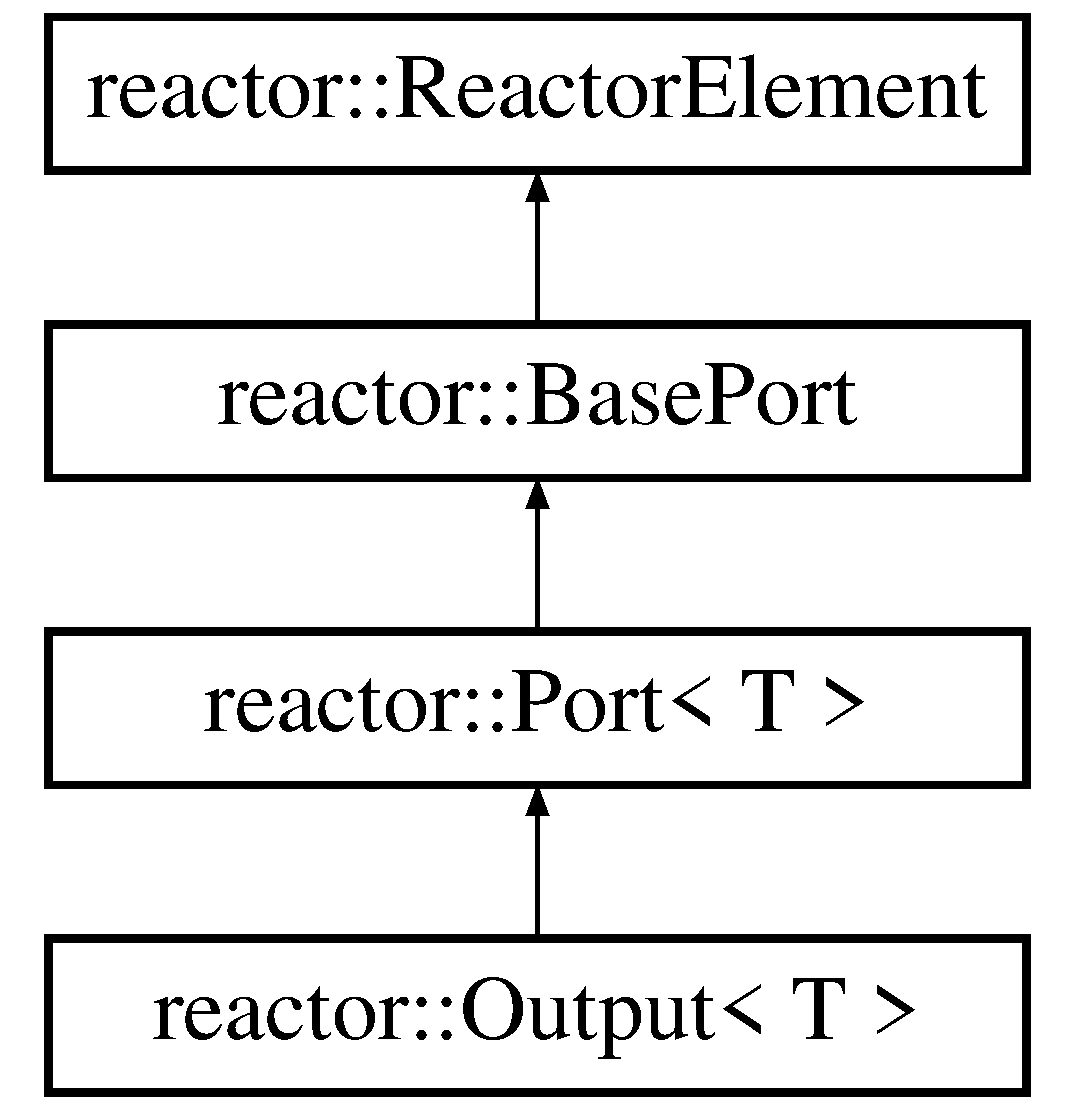
\includegraphics[height=4.000000cm]{classreactor_1_1Output}
\end{center}
\end{figure}
\subsection*{Public Member Functions}
\begin{DoxyCompactItemize}
\item 
\hyperlink{classreactor_1_1Output_a82e2c12d69313c406bf2e0e710295670}{Output} (const std\+::string \&\hyperlink{classreactor_1_1ReactorElement_a99579f61dbaf5d5d98aebfe26eb8bf77}{name}, \hyperlink{classreactor_1_1Reactor}{Reactor} $\ast$\hyperlink{classreactor_1_1ReactorElement_a25bf298de879a82eefc1ba426be05812}{container})
\end{DoxyCompactItemize}
\subsection*{Additional Inherited Members}


\subsection{Constructor \& Destructor Documentation}
\mbox{\Hypertarget{classreactor_1_1Output_a82e2c12d69313c406bf2e0e710295670}\label{classreactor_1_1Output_a82e2c12d69313c406bf2e0e710295670}} 
\index{reactor\+::\+Output@{reactor\+::\+Output}!Output@{Output}}
\index{Output@{Output}!reactor\+::\+Output@{reactor\+::\+Output}}
\subsubsection{\texorpdfstring{Output()}{Output()}}
{\footnotesize\ttfamily template$<$class T $>$ \\
\hyperlink{classreactor_1_1Output}{reactor\+::\+Output}$<$ T $>$\+::\hyperlink{classreactor_1_1Output}{Output} (\begin{DoxyParamCaption}\item[{const std\+::string \&}]{name,  }\item[{\hyperlink{classreactor_1_1Reactor}{Reactor} $\ast$}]{container }\end{DoxyParamCaption})\hspace{0.3cm}{\ttfamily [inline]}}



The documentation for this class was generated from the following file\+:\begin{DoxyCompactItemize}
\item 
/home/runner/work/reactor-\/cpp/reactor-\/cpp/include/reactor-\/cpp/\hyperlink{port_8hh}{port.\+hh}\end{DoxyCompactItemize}

\hypertarget{classreactor_1_1PhysicalAction}{}\section{reactor\+:\+:Physical\+Action$<$ T $>$ Class Template Reference}
\label{classreactor_1_1PhysicalAction}\index{reactor\+::\+Physical\+Action$<$ T $>$@{reactor\+::\+Physical\+Action$<$ T $>$}}


{\ttfamily \#include $<$action.\+hh$>$}

Inheritance diagram for reactor\+:\+:Physical\+Action$<$ T $>$\+:\begin{figure}[H]
\begin{center}
\leavevmode
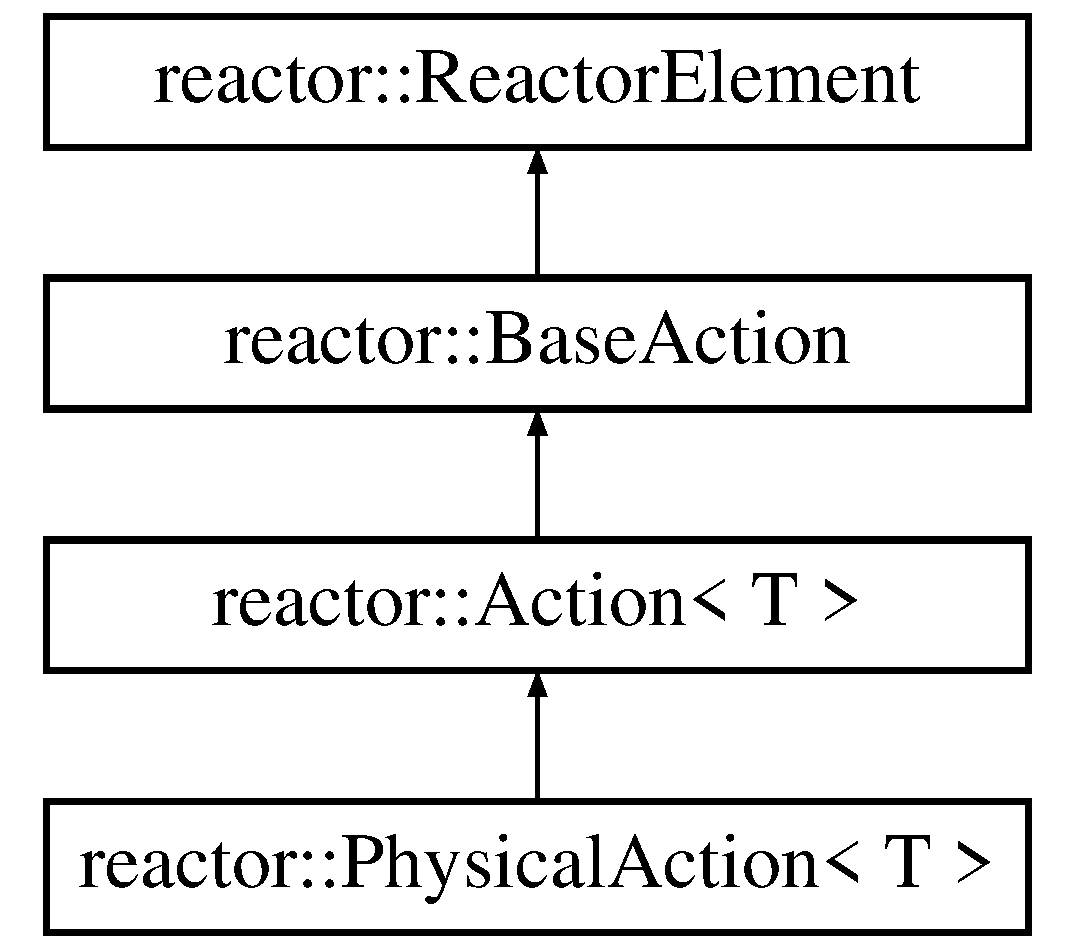
\includegraphics[height=4.000000cm]{classreactor_1_1PhysicalAction}
\end{center}
\end{figure}
\subsection*{Public Member Functions}
\begin{DoxyCompactItemize}
\item 
\hyperlink{classreactor_1_1PhysicalAction_a8b8b1c1b6c701f1cc60254e65e059ec0}{Physical\+Action} (const std\+::string \&\hyperlink{classreactor_1_1ReactorElement_a99579f61dbaf5d5d98aebfe26eb8bf77}{name}, \hyperlink{classreactor_1_1Reactor}{Reactor} $\ast$\hyperlink{classreactor_1_1ReactorElement_a25bf298de879a82eefc1ba426be05812}{container})
\end{DoxyCompactItemize}
\subsection*{Additional Inherited Members}


\subsection{Constructor \& Destructor Documentation}
\mbox{\Hypertarget{classreactor_1_1PhysicalAction_a8b8b1c1b6c701f1cc60254e65e059ec0}\label{classreactor_1_1PhysicalAction_a8b8b1c1b6c701f1cc60254e65e059ec0}} 
\index{reactor\+::\+Physical\+Action@{reactor\+::\+Physical\+Action}!Physical\+Action@{Physical\+Action}}
\index{Physical\+Action@{Physical\+Action}!reactor\+::\+Physical\+Action@{reactor\+::\+Physical\+Action}}
\subsubsection{\texorpdfstring{Physical\+Action()}{PhysicalAction()}}
{\footnotesize\ttfamily template$<$class T $>$ \\
\hyperlink{classreactor_1_1PhysicalAction}{reactor\+::\+Physical\+Action}$<$ T $>$\+::\hyperlink{classreactor_1_1PhysicalAction}{Physical\+Action} (\begin{DoxyParamCaption}\item[{const std\+::string \&}]{name,  }\item[{\hyperlink{classreactor_1_1Reactor}{Reactor} $\ast$}]{container }\end{DoxyParamCaption})\hspace{0.3cm}{\ttfamily [inline]}}



The documentation for this class was generated from the following file\+:\begin{DoxyCompactItemize}
\item 
/home/runner/work/reactor-\/cpp/reactor-\/cpp/include/reactor-\/cpp/\hyperlink{action_8hh}{action.\+hh}\end{DoxyCompactItemize}

\hypertarget{classreactor_1_1Port}{}\section{reactor\+:\+:Port$<$ T $>$ Class Template Reference}
\label{classreactor_1_1Port}\index{reactor\+::\+Port$<$ T $>$@{reactor\+::\+Port$<$ T $>$}}


{\ttfamily \#include $<$fwd.\+hh$>$}

Inheritance diagram for reactor\+:\+:Port$<$ T $>$\+:\begin{figure}[H]
\begin{center}
\leavevmode
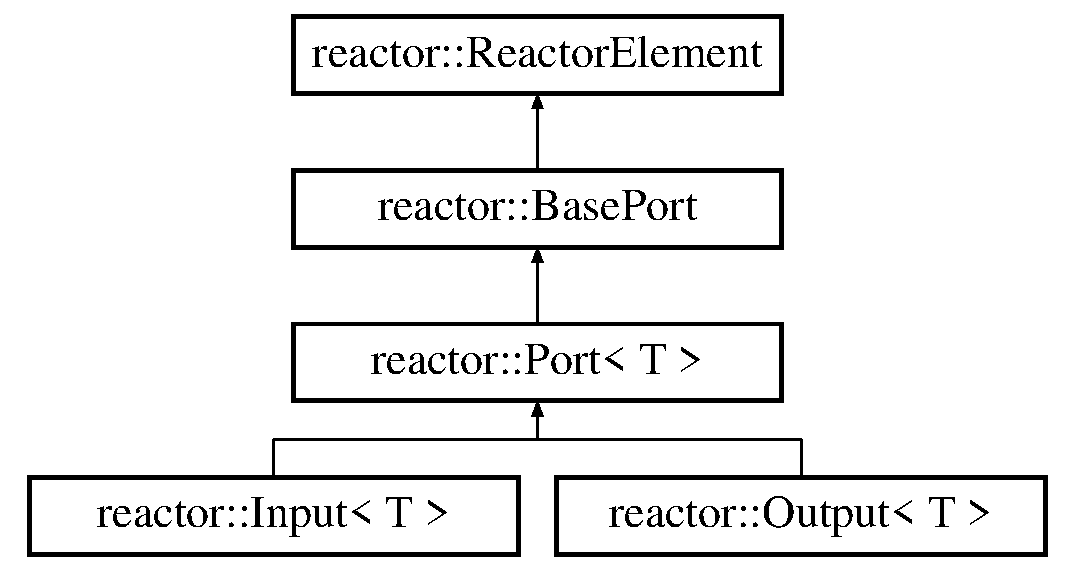
\includegraphics[height=4.000000cm]{classreactor_1_1Port}
\end{center}
\end{figure}
\subsection*{Public Member Functions}
\begin{DoxyCompactItemize}
\item 
\hyperlink{classreactor_1_1Port_a5cd32eff95f2606d94adc482bf6944af}{Port} (const std\+::string \&\hyperlink{classreactor_1_1ReactorElement_a99579f61dbaf5d5d98aebfe26eb8bf77}{name}, \hyperlink{namespacereactor_a08c8e2d85e5bc706b1af8a87e40eec6d}{Port\+Type} \hyperlink{classreactor_1_1BasePort_a9af5e0d55ee1a425b2c5975ab1ca871e}{type}, \hyperlink{classreactor_1_1Reactor}{Reactor} $\ast$\hyperlink{classreactor_1_1ReactorElement_a25bf298de879a82eefc1ba426be05812}{container})
\item 
void \hyperlink{classreactor_1_1Port_a71e1c6fe14a7a6566bc5d5342fa9d16d}{bind\+\_\+to} (\hyperlink{classreactor_1_1Port}{Port}$<$ T $>$ $\ast$port)
\item 
\hyperlink{classreactor_1_1Port}{Port}$<$ T $>$ $\ast$ \hyperlink{classreactor_1_1Port_a22d0ef9cd82989e03a669aeccf8e694a}{typed\+\_\+inward\+\_\+binding} () const
\item 
const std\+::set$<$ \hyperlink{classreactor_1_1Port}{Port}$<$ T $>$ $\ast$ $>$ \& \hyperlink{classreactor_1_1Port_a4d3f681f3f3e0ef75988c3790eb24a17}{typed\+\_\+outward\+\_\+bindings} () const
\item 
void \hyperlink{classreactor_1_1Port_ac3d03f90b425a8656911ed3acf462a4d}{set} (const \hyperlink{classreactor_1_1ImmutableValuePtr}{Immutable\+Value\+Ptr}$<$ T $>$ \&\hyperlink{classreactor_1_1Port_adb40730eea54b529168a70cf8ed933c7}{value\+\_\+ptr})
\item 
void \hyperlink{classreactor_1_1Port_a041b16e47f5b67305ec215513ea92b23}{set} (\hyperlink{classreactor_1_1MutableValuePtr}{Mutable\+Value\+Ptr}$<$ T $>$ \&\&\hyperlink{classreactor_1_1Port_adb40730eea54b529168a70cf8ed933c7}{value\+\_\+ptr})
\item 
void \hyperlink{classreactor_1_1Port_ac75bc82e495f182037d5f7273fc75491}{set} (const T \&value)
\item 
void \hyperlink{classreactor_1_1Port_a9f742e8839c5061c21f890c1ca5fca6b}{set} (T \&\&value)
\item 
void \hyperlink{classreactor_1_1Port_ae182b2b10c53f2a21c424437dfc2b40e}{startup} () override final
\item 
void \hyperlink{classreactor_1_1Port_a3d440102c643fd98d17b4cf8714c910d}{shutdown} () override final
\item 
const \hyperlink{classreactor_1_1ImmutableValuePtr}{Immutable\+Value\+Ptr}$<$ T $>$ \& \hyperlink{classreactor_1_1Port_aac7650bcd4a119063858a0dddb5d58aa}{get} () const
\item 
bool \hyperlink{classreactor_1_1Port_ab4ab58fa62258a9e79b061ecd3f55946}{is\+\_\+present} () const
\end{DoxyCompactItemize}
\subsection*{Private Member Functions}
\begin{DoxyCompactItemize}
\item 
void \hyperlink{classreactor_1_1Port_a05fdfca6fac003412700103e04ee66fd}{cleanup} () override final
\end{DoxyCompactItemize}
\subsection*{Private Attributes}
\begin{DoxyCompactItemize}
\item 
\hyperlink{classreactor_1_1ImmutableValuePtr}{Immutable\+Value\+Ptr}$<$ T $>$ \hyperlink{classreactor_1_1Port_adb40730eea54b529168a70cf8ed933c7}{value\+\_\+ptr} \{nullptr\}
\end{DoxyCompactItemize}
\subsection*{Additional Inherited Members}


\subsection{Constructor \& Destructor Documentation}
\mbox{\Hypertarget{classreactor_1_1Port_a5cd32eff95f2606d94adc482bf6944af}\label{classreactor_1_1Port_a5cd32eff95f2606d94adc482bf6944af}} 
\index{reactor\+::\+Port@{reactor\+::\+Port}!Port@{Port}}
\index{Port@{Port}!reactor\+::\+Port@{reactor\+::\+Port}}
\subsubsection{\texorpdfstring{Port()}{Port()}}
{\footnotesize\ttfamily template$<$class T$>$ \\
\hyperlink{classreactor_1_1Port}{reactor\+::\+Port}$<$ T $>$\+::\hyperlink{classreactor_1_1Port}{Port} (\begin{DoxyParamCaption}\item[{const std\+::string \&}]{name,  }\item[{\hyperlink{namespacereactor_a08c8e2d85e5bc706b1af8a87e40eec6d}{Port\+Type}}]{type,  }\item[{\hyperlink{classreactor_1_1Reactor}{Reactor} $\ast$}]{container }\end{DoxyParamCaption})\hspace{0.3cm}{\ttfamily [inline]}}



\subsection{Member Function Documentation}
\mbox{\Hypertarget{classreactor_1_1Port_a71e1c6fe14a7a6566bc5d5342fa9d16d}\label{classreactor_1_1Port_a71e1c6fe14a7a6566bc5d5342fa9d16d}} 
\index{reactor\+::\+Port@{reactor\+::\+Port}!bind\+\_\+to@{bind\+\_\+to}}
\index{bind\+\_\+to@{bind\+\_\+to}!reactor\+::\+Port@{reactor\+::\+Port}}
\subsubsection{\texorpdfstring{bind\+\_\+to()}{bind\_to()}}
{\footnotesize\ttfamily template$<$class T$>$ \\
void \hyperlink{classreactor_1_1Port}{reactor\+::\+Port}$<$ T $>$\+::bind\+\_\+to (\begin{DoxyParamCaption}\item[{\hyperlink{classreactor_1_1Port}{Port}$<$ T $>$ $\ast$}]{port }\end{DoxyParamCaption})\hspace{0.3cm}{\ttfamily [inline]}}

\mbox{\Hypertarget{classreactor_1_1Port_a05fdfca6fac003412700103e04ee66fd}\label{classreactor_1_1Port_a05fdfca6fac003412700103e04ee66fd}} 
\index{reactor\+::\+Port@{reactor\+::\+Port}!cleanup@{cleanup}}
\index{cleanup@{cleanup}!reactor\+::\+Port@{reactor\+::\+Port}}
\subsubsection{\texorpdfstring{cleanup()}{cleanup()}}
{\footnotesize\ttfamily template$<$class T$>$ \\
void \hyperlink{classreactor_1_1Port}{reactor\+::\+Port}$<$ T $>$\+::cleanup (\begin{DoxyParamCaption}{ }\end{DoxyParamCaption})\hspace{0.3cm}{\ttfamily [inline]}, {\ttfamily [final]}, {\ttfamily [override]}, {\ttfamily [private]}, {\ttfamily [virtual]}}



Implements \hyperlink{classreactor_1_1BasePort_afe81e6747077349da4c420a873783579}{reactor\+::\+Base\+Port}.

\mbox{\Hypertarget{classreactor_1_1Port_aac7650bcd4a119063858a0dddb5d58aa}\label{classreactor_1_1Port_aac7650bcd4a119063858a0dddb5d58aa}} 
\index{reactor\+::\+Port@{reactor\+::\+Port}!get@{get}}
\index{get@{get}!reactor\+::\+Port@{reactor\+::\+Port}}
\subsubsection{\texorpdfstring{get()}{get()}}
{\footnotesize\ttfamily template$<$class T $>$ \\
const \hyperlink{classreactor_1_1ImmutableValuePtr}{Immutable\+Value\+Ptr}$<$ T $>$ \& \hyperlink{classreactor_1_1Port}{reactor\+::\+Port}$<$ T $>$\+::get (\begin{DoxyParamCaption}{ }\end{DoxyParamCaption}) const}

\mbox{\Hypertarget{classreactor_1_1Port_ab4ab58fa62258a9e79b061ecd3f55946}\label{classreactor_1_1Port_ab4ab58fa62258a9e79b061ecd3f55946}} 
\index{reactor\+::\+Port@{reactor\+::\+Port}!is\+\_\+present@{is\+\_\+present}}
\index{is\+\_\+present@{is\+\_\+present}!reactor\+::\+Port@{reactor\+::\+Port}}
\subsubsection{\texorpdfstring{is\+\_\+present()}{is\_present()}}
{\footnotesize\ttfamily template$<$class T $>$ \\
bool \hyperlink{classreactor_1_1Port}{reactor\+::\+Port}$<$ T $>$\+::is\+\_\+present (\begin{DoxyParamCaption}{ }\end{DoxyParamCaption}) const}

\mbox{\Hypertarget{classreactor_1_1Port_ac3d03f90b425a8656911ed3acf462a4d}\label{classreactor_1_1Port_ac3d03f90b425a8656911ed3acf462a4d}} 
\index{reactor\+::\+Port@{reactor\+::\+Port}!set@{set}}
\index{set@{set}!reactor\+::\+Port@{reactor\+::\+Port}}
\subsubsection{\texorpdfstring{set()}{set()}\hspace{0.1cm}{\footnotesize\ttfamily [1/4]}}
{\footnotesize\ttfamily template$<$class T $>$ \\
void \hyperlink{classreactor_1_1Port}{reactor\+::\+Port}$<$ T $>$\+::set (\begin{DoxyParamCaption}\item[{const \hyperlink{classreactor_1_1ImmutableValuePtr}{Immutable\+Value\+Ptr}$<$ T $>$ \&}]{value\+\_\+ptr }\end{DoxyParamCaption})}

\mbox{\Hypertarget{classreactor_1_1Port_a041b16e47f5b67305ec215513ea92b23}\label{classreactor_1_1Port_a041b16e47f5b67305ec215513ea92b23}} 
\index{reactor\+::\+Port@{reactor\+::\+Port}!set@{set}}
\index{set@{set}!reactor\+::\+Port@{reactor\+::\+Port}}
\subsubsection{\texorpdfstring{set()}{set()}\hspace{0.1cm}{\footnotesize\ttfamily [2/4]}}
{\footnotesize\ttfamily template$<$class T$>$ \\
void \hyperlink{classreactor_1_1Port}{reactor\+::\+Port}$<$ T $>$\+::set (\begin{DoxyParamCaption}\item[{\hyperlink{classreactor_1_1MutableValuePtr}{Mutable\+Value\+Ptr}$<$ T $>$ \&\&}]{value\+\_\+ptr }\end{DoxyParamCaption})\hspace{0.3cm}{\ttfamily [inline]}}

\mbox{\Hypertarget{classreactor_1_1Port_ac75bc82e495f182037d5f7273fc75491}\label{classreactor_1_1Port_ac75bc82e495f182037d5f7273fc75491}} 
\index{reactor\+::\+Port@{reactor\+::\+Port}!set@{set}}
\index{set@{set}!reactor\+::\+Port@{reactor\+::\+Port}}
\subsubsection{\texorpdfstring{set()}{set()}\hspace{0.1cm}{\footnotesize\ttfamily [3/4]}}
{\footnotesize\ttfamily template$<$class T$>$ \\
void \hyperlink{classreactor_1_1Port}{reactor\+::\+Port}$<$ T $>$\+::set (\begin{DoxyParamCaption}\item[{const T \&}]{value }\end{DoxyParamCaption})\hspace{0.3cm}{\ttfamily [inline]}}

\mbox{\Hypertarget{classreactor_1_1Port_a9f742e8839c5061c21f890c1ca5fca6b}\label{classreactor_1_1Port_a9f742e8839c5061c21f890c1ca5fca6b}} 
\index{reactor\+::\+Port@{reactor\+::\+Port}!set@{set}}
\index{set@{set}!reactor\+::\+Port@{reactor\+::\+Port}}
\subsubsection{\texorpdfstring{set()}{set()}\hspace{0.1cm}{\footnotesize\ttfamily [4/4]}}
{\footnotesize\ttfamily template$<$class T$>$ \\
void \hyperlink{classreactor_1_1Port}{reactor\+::\+Port}$<$ T $>$\+::set (\begin{DoxyParamCaption}\item[{T \&\&}]{value }\end{DoxyParamCaption})\hspace{0.3cm}{\ttfamily [inline]}}

\mbox{\Hypertarget{classreactor_1_1Port_a3d440102c643fd98d17b4cf8714c910d}\label{classreactor_1_1Port_a3d440102c643fd98d17b4cf8714c910d}} 
\index{reactor\+::\+Port@{reactor\+::\+Port}!shutdown@{shutdown}}
\index{shutdown@{shutdown}!reactor\+::\+Port@{reactor\+::\+Port}}
\subsubsection{\texorpdfstring{shutdown()}{shutdown()}}
{\footnotesize\ttfamily template$<$class T$>$ \\
void \hyperlink{classreactor_1_1Port}{reactor\+::\+Port}$<$ T $>$\+::shutdown (\begin{DoxyParamCaption}{ }\end{DoxyParamCaption})\hspace{0.3cm}{\ttfamily [inline]}, {\ttfamily [final]}, {\ttfamily [override]}, {\ttfamily [virtual]}}



Implements \hyperlink{classreactor_1_1ReactorElement_a8fce084bef582156979ebba56737e907}{reactor\+::\+Reactor\+Element}.

\mbox{\Hypertarget{classreactor_1_1Port_ae182b2b10c53f2a21c424437dfc2b40e}\label{classreactor_1_1Port_ae182b2b10c53f2a21c424437dfc2b40e}} 
\index{reactor\+::\+Port@{reactor\+::\+Port}!startup@{startup}}
\index{startup@{startup}!reactor\+::\+Port@{reactor\+::\+Port}}
\subsubsection{\texorpdfstring{startup()}{startup()}}
{\footnotesize\ttfamily template$<$class T$>$ \\
void \hyperlink{classreactor_1_1Port}{reactor\+::\+Port}$<$ T $>$\+::startup (\begin{DoxyParamCaption}{ }\end{DoxyParamCaption})\hspace{0.3cm}{\ttfamily [inline]}, {\ttfamily [final]}, {\ttfamily [override]}, {\ttfamily [virtual]}}



Implements \hyperlink{classreactor_1_1ReactorElement_a8cb574cb20ff963903ad905fb0a157e3}{reactor\+::\+Reactor\+Element}.

\mbox{\Hypertarget{classreactor_1_1Port_a22d0ef9cd82989e03a669aeccf8e694a}\label{classreactor_1_1Port_a22d0ef9cd82989e03a669aeccf8e694a}} 
\index{reactor\+::\+Port@{reactor\+::\+Port}!typed\+\_\+inward\+\_\+binding@{typed\+\_\+inward\+\_\+binding}}
\index{typed\+\_\+inward\+\_\+binding@{typed\+\_\+inward\+\_\+binding}!reactor\+::\+Port@{reactor\+::\+Port}}
\subsubsection{\texorpdfstring{typed\+\_\+inward\+\_\+binding()}{typed\_inward\_binding()}}
{\footnotesize\ttfamily template$<$class T $>$ \\
\hyperlink{classreactor_1_1Port}{Port}$<$ T $>$ $\ast$ \hyperlink{classreactor_1_1Port}{reactor\+::\+Port}$<$ T $>$\+::typed\+\_\+inward\+\_\+binding (\begin{DoxyParamCaption}{ }\end{DoxyParamCaption}) const}

\mbox{\Hypertarget{classreactor_1_1Port_a4d3f681f3f3e0ef75988c3790eb24a17}\label{classreactor_1_1Port_a4d3f681f3f3e0ef75988c3790eb24a17}} 
\index{reactor\+::\+Port@{reactor\+::\+Port}!typed\+\_\+outward\+\_\+bindings@{typed\+\_\+outward\+\_\+bindings}}
\index{typed\+\_\+outward\+\_\+bindings@{typed\+\_\+outward\+\_\+bindings}!reactor\+::\+Port@{reactor\+::\+Port}}
\subsubsection{\texorpdfstring{typed\+\_\+outward\+\_\+bindings()}{typed\_outward\_bindings()}}
{\footnotesize\ttfamily template$<$class T $>$ \\
const std\+::set$<$ \hyperlink{classreactor_1_1Port}{Port}$<$ T $>$ $\ast$ $>$ \& \hyperlink{classreactor_1_1Port}{reactor\+::\+Port}$<$ T $>$\+::typed\+\_\+outward\+\_\+bindings (\begin{DoxyParamCaption}{ }\end{DoxyParamCaption}) const}



\subsection{Member Data Documentation}
\mbox{\Hypertarget{classreactor_1_1Port_adb40730eea54b529168a70cf8ed933c7}\label{classreactor_1_1Port_adb40730eea54b529168a70cf8ed933c7}} 
\index{reactor\+::\+Port@{reactor\+::\+Port}!value\+\_\+ptr@{value\+\_\+ptr}}
\index{value\+\_\+ptr@{value\+\_\+ptr}!reactor\+::\+Port@{reactor\+::\+Port}}
\subsubsection{\texorpdfstring{value\+\_\+ptr}{value\_ptr}}
{\footnotesize\ttfamily template$<$class T$>$ \\
\hyperlink{classreactor_1_1ImmutableValuePtr}{Immutable\+Value\+Ptr}$<$T$>$ \hyperlink{classreactor_1_1Port}{reactor\+::\+Port}$<$ T $>$\+::value\+\_\+ptr \{nullptr\}\hspace{0.3cm}{\ttfamily [private]}}



The documentation for this class was generated from the following files\+:\begin{DoxyCompactItemize}
\item 
/home/runner/work/reactor-\/cpp/reactor-\/cpp/include/reactor-\/cpp/\hyperlink{fwd_8hh}{fwd.\+hh}\item 
/home/runner/work/reactor-\/cpp/reactor-\/cpp/include/reactor-\/cpp/\hyperlink{port_8hh}{port.\+hh}\item 
/home/runner/work/reactor-\/cpp/reactor-\/cpp/include/reactor-\/cpp/impl/\hyperlink{port__impl_8hh}{port\+\_\+impl.\+hh}\end{DoxyCompactItemize}

\hypertarget{classreactor_1_1Port_3_01void_01_4}{}\section{reactor\+:\+:Port$<$ void $>$ Class Template Reference}
\label{classreactor_1_1Port_3_01void_01_4}\index{reactor\+::\+Port$<$ void $>$@{reactor\+::\+Port$<$ void $>$}}


{\ttfamily \#include $<$port.\+hh$>$}

Inheritance diagram for reactor\+:\+:Port$<$ void $>$\+:\begin{figure}[H]
\begin{center}
\leavevmode
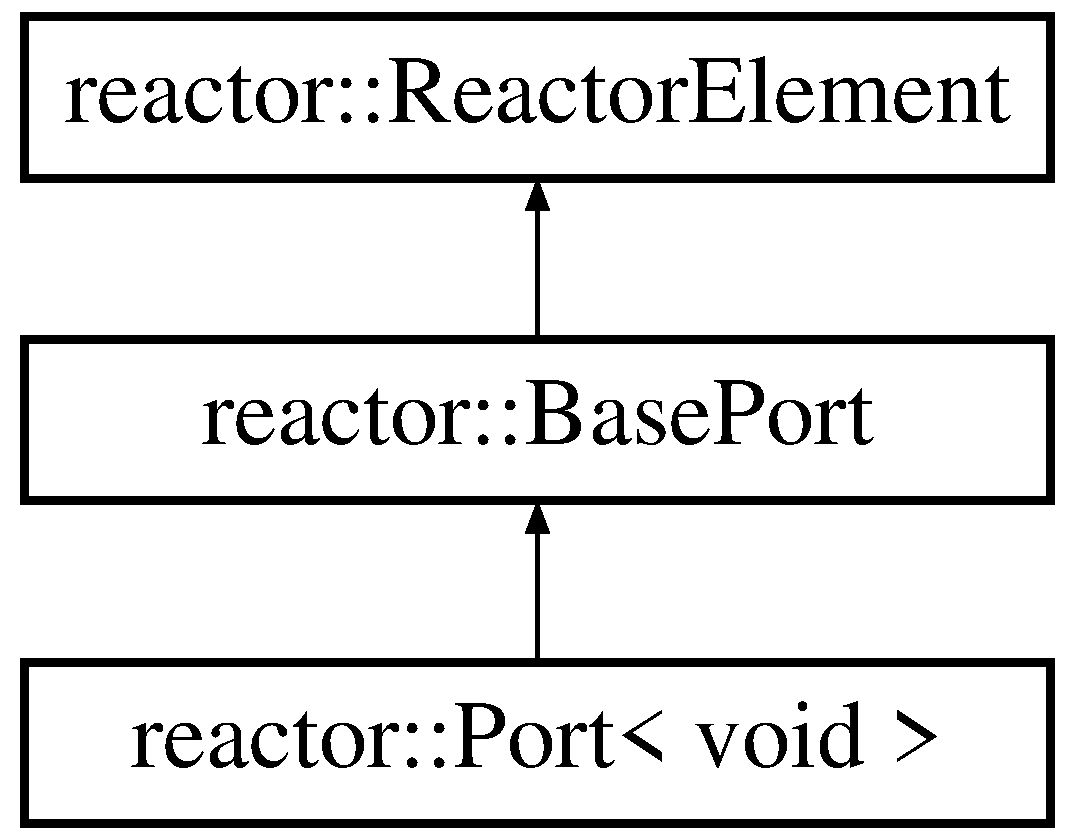
\includegraphics[height=3.000000cm]{classreactor_1_1Port_3_01void_01_4}
\end{center}
\end{figure}
\subsection*{Public Member Functions}
\begin{DoxyCompactItemize}
\item 
\hyperlink{classreactor_1_1Port_3_01void_01_4_a2114887bc779a8f035dcf0e21eabd5fd}{Port} (const std\+::string \&\hyperlink{classreactor_1_1ReactorElement_a99579f61dbaf5d5d98aebfe26eb8bf77}{name}, \hyperlink{namespacereactor_a08c8e2d85e5bc706b1af8a87e40eec6d}{Port\+Type} \hyperlink{classreactor_1_1BasePort_a9af5e0d55ee1a425b2c5975ab1ca871e}{type}, \hyperlink{classreactor_1_1Reactor}{Reactor} $\ast$\hyperlink{classreactor_1_1ReactorElement_a25bf298de879a82eefc1ba426be05812}{container})
\item 
void \hyperlink{classreactor_1_1Port_3_01void_01_4_a86c25528d080fe3d1bba83878fd53860}{bind\+\_\+to} (\hyperlink{classreactor_1_1Port}{Port}$<$ void $>$ $\ast$port)
\item 
\hyperlink{classreactor_1_1Port}{Port}$<$ void $>$ $\ast$ \hyperlink{classreactor_1_1Port_3_01void_01_4_aa50594b9d98fa93219adf8330ed76131}{typed\+\_\+inward\+\_\+binding} () const
\item 
const std\+::set$<$ \hyperlink{classreactor_1_1Port}{Port}$<$ void $>$ $\ast$ $>$ \& \hyperlink{classreactor_1_1Port_3_01void_01_4_a8f9bdc0b6bace7d1a05615b28cf43717}{typed\+\_\+outward\+\_\+bindings} () const
\item 
void \hyperlink{classreactor_1_1Port_3_01void_01_4_afe579f1f5b555a15703c9a05d28bea03}{set} ()
\item 
bool \hyperlink{classreactor_1_1Port_3_01void_01_4_a9f7a92606f6f4600b85fd4680de7007d}{is\+\_\+present} () const
\item 
void \hyperlink{classreactor_1_1Port_3_01void_01_4_a3a84b8d17b1a43197a753847b0df1777}{startup} () override final
\item 
void \hyperlink{classreactor_1_1Port_3_01void_01_4_ad7d9028d091509215b3685e4af95cb03}{shutdown} () override final
\end{DoxyCompactItemize}
\subsection*{Private Member Functions}
\begin{DoxyCompactItemize}
\item 
void \hyperlink{classreactor_1_1Port_3_01void_01_4_aedf8266554cde75e236451d8c512e4c8}{cleanup} () override final
\end{DoxyCompactItemize}
\subsection*{Private Attributes}
\begin{DoxyCompactItemize}
\item 
bool \hyperlink{classreactor_1_1Port_3_01void_01_4_aa9ab4e50d097ed98354eb6508f4e7085}{present} \{false\}
\end{DoxyCompactItemize}
\subsection*{Additional Inherited Members}


\subsection{Constructor \& Destructor Documentation}
\mbox{\Hypertarget{classreactor_1_1Port_3_01void_01_4_a2114887bc779a8f035dcf0e21eabd5fd}\label{classreactor_1_1Port_3_01void_01_4_a2114887bc779a8f035dcf0e21eabd5fd}} 
\index{reactor\+::\+Port$<$ void $>$@{reactor\+::\+Port$<$ void $>$}!Port@{Port}}
\index{Port@{Port}!reactor\+::\+Port$<$ void $>$@{reactor\+::\+Port$<$ void $>$}}
\subsubsection{\texorpdfstring{Port()}{Port()}}
{\footnotesize\ttfamily \hyperlink{classreactor_1_1Port}{reactor\+::\+Port}$<$ void $>$\+::\hyperlink{classreactor_1_1Port}{Port} (\begin{DoxyParamCaption}\item[{const std\+::string \&}]{name,  }\item[{\hyperlink{namespacereactor_a08c8e2d85e5bc706b1af8a87e40eec6d}{Port\+Type}}]{type,  }\item[{\hyperlink{classreactor_1_1Reactor}{Reactor} $\ast$}]{container }\end{DoxyParamCaption})\hspace{0.3cm}{\ttfamily [inline]}}



\subsection{Member Function Documentation}
\mbox{\Hypertarget{classreactor_1_1Port_3_01void_01_4_a86c25528d080fe3d1bba83878fd53860}\label{classreactor_1_1Port_3_01void_01_4_a86c25528d080fe3d1bba83878fd53860}} 
\index{reactor\+::\+Port$<$ void $>$@{reactor\+::\+Port$<$ void $>$}!bind\+\_\+to@{bind\+\_\+to}}
\index{bind\+\_\+to@{bind\+\_\+to}!reactor\+::\+Port$<$ void $>$@{reactor\+::\+Port$<$ void $>$}}
\subsubsection{\texorpdfstring{bind\+\_\+to()}{bind\_to()}}
{\footnotesize\ttfamily void \hyperlink{classreactor_1_1Port}{reactor\+::\+Port}$<$ void $>$\+::bind\+\_\+to (\begin{DoxyParamCaption}\item[{\hyperlink{classreactor_1_1Port}{Port}$<$ void $>$ $\ast$}]{port }\end{DoxyParamCaption})\hspace{0.3cm}{\ttfamily [inline]}}

\mbox{\Hypertarget{classreactor_1_1Port_3_01void_01_4_aedf8266554cde75e236451d8c512e4c8}\label{classreactor_1_1Port_3_01void_01_4_aedf8266554cde75e236451d8c512e4c8}} 
\index{reactor\+::\+Port$<$ void $>$@{reactor\+::\+Port$<$ void $>$}!cleanup@{cleanup}}
\index{cleanup@{cleanup}!reactor\+::\+Port$<$ void $>$@{reactor\+::\+Port$<$ void $>$}}
\subsubsection{\texorpdfstring{cleanup()}{cleanup()}}
{\footnotesize\ttfamily void \hyperlink{classreactor_1_1Port}{reactor\+::\+Port}$<$ void $>$\+::cleanup (\begin{DoxyParamCaption}{ }\end{DoxyParamCaption})\hspace{0.3cm}{\ttfamily [inline]}, {\ttfamily [final]}, {\ttfamily [override]}, {\ttfamily [private]}, {\ttfamily [virtual]}}



Implements \hyperlink{classreactor_1_1BasePort_afe81e6747077349da4c420a873783579}{reactor\+::\+Base\+Port}.

\mbox{\Hypertarget{classreactor_1_1Port_3_01void_01_4_a9f7a92606f6f4600b85fd4680de7007d}\label{classreactor_1_1Port_3_01void_01_4_a9f7a92606f6f4600b85fd4680de7007d}} 
\index{reactor\+::\+Port$<$ void $>$@{reactor\+::\+Port$<$ void $>$}!is\+\_\+present@{is\+\_\+present}}
\index{is\+\_\+present@{is\+\_\+present}!reactor\+::\+Port$<$ void $>$@{reactor\+::\+Port$<$ void $>$}}
\subsubsection{\texorpdfstring{is\+\_\+present()}{is\_present()}}
{\footnotesize\ttfamily bool \hyperlink{classreactor_1_1Port}{reactor\+::\+Port}$<$ void $>$\+::is\+\_\+present (\begin{DoxyParamCaption}{ }\end{DoxyParamCaption}) const}

\mbox{\Hypertarget{classreactor_1_1Port_3_01void_01_4_afe579f1f5b555a15703c9a05d28bea03}\label{classreactor_1_1Port_3_01void_01_4_afe579f1f5b555a15703c9a05d28bea03}} 
\index{reactor\+::\+Port$<$ void $>$@{reactor\+::\+Port$<$ void $>$}!set@{set}}
\index{set@{set}!reactor\+::\+Port$<$ void $>$@{reactor\+::\+Port$<$ void $>$}}
\subsubsection{\texorpdfstring{set()}{set()}}
{\footnotesize\ttfamily void \hyperlink{classreactor_1_1Port}{reactor\+::\+Port}$<$ void $>$\+::set (\begin{DoxyParamCaption}{ }\end{DoxyParamCaption})}

\mbox{\Hypertarget{classreactor_1_1Port_3_01void_01_4_ad7d9028d091509215b3685e4af95cb03}\label{classreactor_1_1Port_3_01void_01_4_ad7d9028d091509215b3685e4af95cb03}} 
\index{reactor\+::\+Port$<$ void $>$@{reactor\+::\+Port$<$ void $>$}!shutdown@{shutdown}}
\index{shutdown@{shutdown}!reactor\+::\+Port$<$ void $>$@{reactor\+::\+Port$<$ void $>$}}
\subsubsection{\texorpdfstring{shutdown()}{shutdown()}}
{\footnotesize\ttfamily void \hyperlink{classreactor_1_1Port}{reactor\+::\+Port}$<$ void $>$\+::shutdown (\begin{DoxyParamCaption}{ }\end{DoxyParamCaption})\hspace{0.3cm}{\ttfamily [inline]}, {\ttfamily [final]}, {\ttfamily [override]}, {\ttfamily [virtual]}}



Implements \hyperlink{classreactor_1_1ReactorElement_a8fce084bef582156979ebba56737e907}{reactor\+::\+Reactor\+Element}.

\mbox{\Hypertarget{classreactor_1_1Port_3_01void_01_4_a3a84b8d17b1a43197a753847b0df1777}\label{classreactor_1_1Port_3_01void_01_4_a3a84b8d17b1a43197a753847b0df1777}} 
\index{reactor\+::\+Port$<$ void $>$@{reactor\+::\+Port$<$ void $>$}!startup@{startup}}
\index{startup@{startup}!reactor\+::\+Port$<$ void $>$@{reactor\+::\+Port$<$ void $>$}}
\subsubsection{\texorpdfstring{startup()}{startup()}}
{\footnotesize\ttfamily void \hyperlink{classreactor_1_1Port}{reactor\+::\+Port}$<$ void $>$\+::startup (\begin{DoxyParamCaption}{ }\end{DoxyParamCaption})\hspace{0.3cm}{\ttfamily [inline]}, {\ttfamily [final]}, {\ttfamily [override]}, {\ttfamily [virtual]}}



Implements \hyperlink{classreactor_1_1ReactorElement_a8cb574cb20ff963903ad905fb0a157e3}{reactor\+::\+Reactor\+Element}.

\mbox{\Hypertarget{classreactor_1_1Port_3_01void_01_4_aa50594b9d98fa93219adf8330ed76131}\label{classreactor_1_1Port_3_01void_01_4_aa50594b9d98fa93219adf8330ed76131}} 
\index{reactor\+::\+Port$<$ void $>$@{reactor\+::\+Port$<$ void $>$}!typed\+\_\+inward\+\_\+binding@{typed\+\_\+inward\+\_\+binding}}
\index{typed\+\_\+inward\+\_\+binding@{typed\+\_\+inward\+\_\+binding}!reactor\+::\+Port$<$ void $>$@{reactor\+::\+Port$<$ void $>$}}
\subsubsection{\texorpdfstring{typed\+\_\+inward\+\_\+binding()}{typed\_inward\_binding()}}
{\footnotesize\ttfamily \hyperlink{classreactor_1_1Port}{Port}$<$ void $>$ $\ast$ \hyperlink{classreactor_1_1Port}{reactor\+::\+Port}$<$ void $>$\+::typed\+\_\+inward\+\_\+binding (\begin{DoxyParamCaption}{ }\end{DoxyParamCaption}) const}

\mbox{\Hypertarget{classreactor_1_1Port_3_01void_01_4_a8f9bdc0b6bace7d1a05615b28cf43717}\label{classreactor_1_1Port_3_01void_01_4_a8f9bdc0b6bace7d1a05615b28cf43717}} 
\index{reactor\+::\+Port$<$ void $>$@{reactor\+::\+Port$<$ void $>$}!typed\+\_\+outward\+\_\+bindings@{typed\+\_\+outward\+\_\+bindings}}
\index{typed\+\_\+outward\+\_\+bindings@{typed\+\_\+outward\+\_\+bindings}!reactor\+::\+Port$<$ void $>$@{reactor\+::\+Port$<$ void $>$}}
\subsubsection{\texorpdfstring{typed\+\_\+outward\+\_\+bindings()}{typed\_outward\_bindings()}}
{\footnotesize\ttfamily const std\+::set$<$ \hyperlink{classreactor_1_1Port}{Port}$<$ void $>$ $\ast$ $>$ \& \hyperlink{classreactor_1_1Port}{reactor\+::\+Port}$<$ void $>$\+::typed\+\_\+outward\+\_\+bindings (\begin{DoxyParamCaption}{ }\end{DoxyParamCaption}) const}



\subsection{Member Data Documentation}
\mbox{\Hypertarget{classreactor_1_1Port_3_01void_01_4_aa9ab4e50d097ed98354eb6508f4e7085}\label{classreactor_1_1Port_3_01void_01_4_aa9ab4e50d097ed98354eb6508f4e7085}} 
\index{reactor\+::\+Port$<$ void $>$@{reactor\+::\+Port$<$ void $>$}!present@{present}}
\index{present@{present}!reactor\+::\+Port$<$ void $>$@{reactor\+::\+Port$<$ void $>$}}
\subsubsection{\texorpdfstring{present}{present}}
{\footnotesize\ttfamily bool \hyperlink{classreactor_1_1Port}{reactor\+::\+Port}$<$ void $>$\+::present \{false\}\hspace{0.3cm}{\ttfamily [private]}}



The documentation for this class was generated from the following files\+:\begin{DoxyCompactItemize}
\item 
/home/runner/work/reactor-\/cpp/reactor-\/cpp/include/reactor-\/cpp/\hyperlink{port_8hh}{port.\+hh}\item 
/home/runner/work/reactor-\/cpp/reactor-\/cpp/lib/\hyperlink{port_8cc}{port.\+cc}\end{DoxyCompactItemize}

\hypertarget{classreactor_1_1Reaction}{}\section{reactor\+:\+:Reaction Class Reference}
\label{classreactor_1_1Reaction}\index{reactor\+::\+Reaction@{reactor\+::\+Reaction}}


{\ttfamily \#include $<$reaction.\+hh$>$}

Inheritance diagram for reactor\+:\+:Reaction\+:\begin{figure}[H]
\begin{center}
\leavevmode
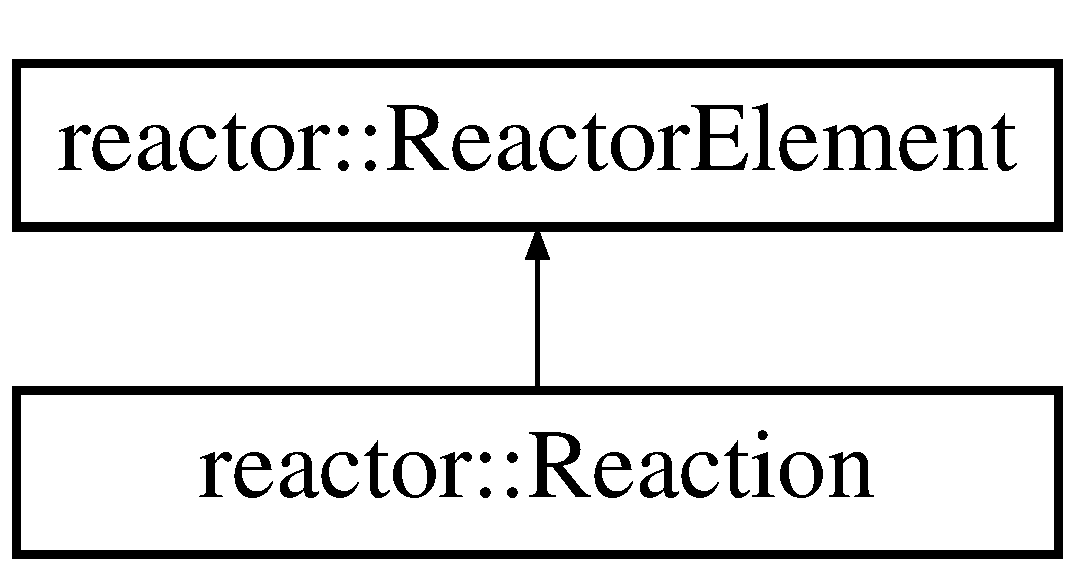
\includegraphics[height=2.000000cm]{classreactor_1_1Reaction}
\end{center}
\end{figure}
\subsection*{Public Member Functions}
\begin{DoxyCompactItemize}
\item 
\hyperlink{classreactor_1_1Reaction_a5d6b7249352ddb4c0fdde855fea2b191}{Reaction} (const std\+::string \&\hyperlink{classreactor_1_1ReactorElement_a99579f61dbaf5d5d98aebfe26eb8bf77}{name}, int \hyperlink{classreactor_1_1Reaction_a5fb22f21bbdf4f0303bb036d8afdf91e}{priority}, \hyperlink{classreactor_1_1Reactor}{Reactor} $\ast$\hyperlink{classreactor_1_1ReactorElement_a25bf298de879a82eefc1ba426be05812}{container}, std\+::function$<$ void(void)$>$ \hyperlink{classreactor_1_1Reaction_aca4e15066e159bf9c009c87f5ec11180}{body})
\item 
virtual \hyperlink{classreactor_1_1Reaction_aa532060472706da66267b8a6ac6a88ad}{$\sim$\+Reaction} ()
\item 
void \hyperlink{classreactor_1_1Reaction_a5733b0fa4559a2221f3b32f2ce12947a}{declare\+\_\+trigger} (\hyperlink{classreactor_1_1BaseAction}{Base\+Action} $\ast$action)
\item 
void \hyperlink{classreactor_1_1Reaction_a8e4980f5e05c8bedef5d8c7f9c7ec142}{declare\+\_\+trigger} (\hyperlink{classreactor_1_1BasePort}{Base\+Port} $\ast$port)
\item 
void \hyperlink{classreactor_1_1Reaction_acf9c9897530f4a02bdec524456965315}{declare\+\_\+scheduable\+\_\+action} (\hyperlink{classreactor_1_1BaseAction}{Base\+Action} $\ast$action)
\item 
void \hyperlink{classreactor_1_1Reaction_a9808e5479e13e76d2d7151c7afef280b}{declare\+\_\+antidependency} (\hyperlink{classreactor_1_1BasePort}{Base\+Port} $\ast$port)
\item 
void \hyperlink{classreactor_1_1Reaction_a1c0a84a9e241998cfb19377052fff856}{declare\+\_\+dependency} (\hyperlink{classreactor_1_1BasePort}{Base\+Port} $\ast$port)
\item 
const auto \& \hyperlink{classreactor_1_1Reaction_a1f2f04c900ead25ec920bdede95fd8fd}{action\+\_\+triggers} () const
\item 
const auto \& \hyperlink{classreactor_1_1Reaction_af722cdf4be08668017a783ceccdcfa5a}{port\+\_\+triggers} () const
\item 
const auto \& \hyperlink{classreactor_1_1Reaction_aacb42127c5fe2f11f166169ae6ebc56b}{antidependencies} () const
\item 
const auto \& \hyperlink{classreactor_1_1Reaction_a3cc0fd73eab307c5f4110213cc9e2b20}{dependencies} () const
\item 
const auto \& \hyperlink{classreactor_1_1Reaction_a0d7ebde1c7684c553925185299b4a872}{scheduable\+\_\+actions} () const
\item 
int \hyperlink{classreactor_1_1Reaction_a5fb22f21bbdf4f0303bb036d8afdf91e}{priority} () const
\item 
void \hyperlink{classreactor_1_1Reaction_a504359d36ac61662668787c9b650c314}{startup} () override final
\item 
void \hyperlink{classreactor_1_1Reaction_ae4011cf04c0d7158ffd1360fb00bcc29}{shutdown} () override final
\item 
void \hyperlink{classreactor_1_1Reaction_a33e0f5fff73c2908547dd1c65219ded6}{trigger} ()
\item 
{\footnotesize template$<$class Dur $>$ }\\void \hyperlink{classreactor_1_1Reaction_a2fc16f7109c4dddc894d54477fd96aed}{set\+\_\+deadline} (Dur dl, std\+::function$<$ void(void)$>$ handler)
\item 
bool \hyperlink{classreactor_1_1Reaction_a783267d5eeaba65163c5be768930ce05}{has\+\_\+deadline} () const
\item 
void \hyperlink{classreactor_1_1Reaction_a17c9cece9fe948cc5b85e8b9bd8f77c3}{set\+\_\+index} (unsigned \hyperlink{classreactor_1_1Reaction_a3bff1f3f5ad6094ba8d121c1657b3ef2}{index})
\item 
unsigned \hyperlink{classreactor_1_1Reaction_a3bff1f3f5ad6094ba8d121c1657b3ef2}{index} () const
\end{DoxyCompactItemize}
\subsection*{Private Member Functions}
\begin{DoxyCompactItemize}
\item 
void \hyperlink{classreactor_1_1Reaction_a8fee209cdb1d77185b0e9a992c044b71}{set\+\_\+deadline\+\_\+impl} (\hyperlink{namespacereactor_aa8375b807a80703545664096c5b5b779}{Duration} \hyperlink{classreactor_1_1Reaction_aa8704882695ff4a0b9ab7d866b2f79b1}{deadline}, std\+::function$<$ void(void)$>$ handler)
\end{DoxyCompactItemize}
\subsection*{Private Attributes}
\begin{DoxyCompactItemize}
\item 
std\+::set$<$ \hyperlink{classreactor_1_1BaseAction}{Base\+Action} $\ast$ $>$ \hyperlink{classreactor_1_1Reaction_ae78a33de1d45afcfecf0297d79841028}{\+\_\+action\+\_\+triggers}
\item 
std\+::set$<$ \hyperlink{classreactor_1_1BaseAction}{Base\+Action} $\ast$ $>$ \hyperlink{classreactor_1_1Reaction_af5baa35846e71e7c0fc2f0fc4de14c84}{\+\_\+scheduable\+\_\+actions}
\item 
std\+::set$<$ \hyperlink{classreactor_1_1BasePort}{Base\+Port} $\ast$ $>$ \hyperlink{classreactor_1_1Reaction_a963d6a24063a5dae91f5e74ec9db00bd}{\+\_\+port\+\_\+triggers}
\item 
std\+::set$<$ \hyperlink{classreactor_1_1BasePort}{Base\+Port} $\ast$ $>$ \hyperlink{classreactor_1_1Reaction_aed9f1447027533b2b0c2ae77b933e546}{\+\_\+antidependencies}
\item 
std\+::set$<$ \hyperlink{classreactor_1_1BasePort}{Base\+Port} $\ast$ $>$ \hyperlink{classreactor_1_1Reaction_a5f1411deb1e0d3ab353f4e332a027556}{\+\_\+dependencies}
\item 
const int \hyperlink{classreactor_1_1Reaction_aea5d30c041bc7adb9ab986212bed6af4}{\+\_\+priority}
\item 
unsigned \hyperlink{classreactor_1_1Reaction_a833e6769a31f10fd46399bcaa3b54038}{\+\_\+index}
\item 
std\+::function$<$ void(void)$>$ \hyperlink{classreactor_1_1Reaction_aca4e15066e159bf9c009c87f5ec11180}{body}
\item 
\hyperlink{namespacereactor_aa8375b807a80703545664096c5b5b779}{Duration} \hyperlink{classreactor_1_1Reaction_aa8704882695ff4a0b9ab7d866b2f79b1}{deadline} \{Duration\+::zero()\}
\item 
std\+::function$<$ void(void)$>$ \hyperlink{classreactor_1_1Reaction_aaa6466268aa7e9ba823a7a45b7c75667}{deadline\+\_\+handler} \{nullptr\}
\end{DoxyCompactItemize}
\subsection*{Additional Inherited Members}


\subsection{Constructor \& Destructor Documentation}
\mbox{\Hypertarget{classreactor_1_1Reaction_a5d6b7249352ddb4c0fdde855fea2b191}\label{classreactor_1_1Reaction_a5d6b7249352ddb4c0fdde855fea2b191}} 
\index{reactor\+::\+Reaction@{reactor\+::\+Reaction}!Reaction@{Reaction}}
\index{Reaction@{Reaction}!reactor\+::\+Reaction@{reactor\+::\+Reaction}}
\subsubsection{\texorpdfstring{Reaction()}{Reaction()}}
{\footnotesize\ttfamily reactor\+::\+Reaction\+::\+Reaction (\begin{DoxyParamCaption}\item[{const std\+::string \&}]{name,  }\item[{int}]{priority,  }\item[{\hyperlink{classreactor_1_1Reactor}{Reactor} $\ast$}]{container,  }\item[{std\+::function$<$ void(void)$>$}]{body }\end{DoxyParamCaption})}

\mbox{\Hypertarget{classreactor_1_1Reaction_aa532060472706da66267b8a6ac6a88ad}\label{classreactor_1_1Reaction_aa532060472706da66267b8a6ac6a88ad}} 
\index{reactor\+::\+Reaction@{reactor\+::\+Reaction}!````~Reaction@{$\sim$\+Reaction}}
\index{````~Reaction@{$\sim$\+Reaction}!reactor\+::\+Reaction@{reactor\+::\+Reaction}}
\subsubsection{\texorpdfstring{$\sim$\+Reaction()}{~Reaction()}}
{\footnotesize\ttfamily virtual reactor\+::\+Reaction\+::$\sim$\+Reaction (\begin{DoxyParamCaption}{ }\end{DoxyParamCaption})\hspace{0.3cm}{\ttfamily [inline]}, {\ttfamily [virtual]}}



\subsection{Member Function Documentation}
\mbox{\Hypertarget{classreactor_1_1Reaction_a1f2f04c900ead25ec920bdede95fd8fd}\label{classreactor_1_1Reaction_a1f2f04c900ead25ec920bdede95fd8fd}} 
\index{reactor\+::\+Reaction@{reactor\+::\+Reaction}!action\+\_\+triggers@{action\+\_\+triggers}}
\index{action\+\_\+triggers@{action\+\_\+triggers}!reactor\+::\+Reaction@{reactor\+::\+Reaction}}
\subsubsection{\texorpdfstring{action\+\_\+triggers()}{action\_triggers()}}
{\footnotesize\ttfamily const auto\& reactor\+::\+Reaction\+::action\+\_\+triggers (\begin{DoxyParamCaption}{ }\end{DoxyParamCaption}) const\hspace{0.3cm}{\ttfamily [inline]}}

\mbox{\Hypertarget{classreactor_1_1Reaction_aacb42127c5fe2f11f166169ae6ebc56b}\label{classreactor_1_1Reaction_aacb42127c5fe2f11f166169ae6ebc56b}} 
\index{reactor\+::\+Reaction@{reactor\+::\+Reaction}!antidependencies@{antidependencies}}
\index{antidependencies@{antidependencies}!reactor\+::\+Reaction@{reactor\+::\+Reaction}}
\subsubsection{\texorpdfstring{antidependencies()}{antidependencies()}}
{\footnotesize\ttfamily const auto\& reactor\+::\+Reaction\+::antidependencies (\begin{DoxyParamCaption}{ }\end{DoxyParamCaption}) const\hspace{0.3cm}{\ttfamily [inline]}}

\mbox{\Hypertarget{classreactor_1_1Reaction_a9808e5479e13e76d2d7151c7afef280b}\label{classreactor_1_1Reaction_a9808e5479e13e76d2d7151c7afef280b}} 
\index{reactor\+::\+Reaction@{reactor\+::\+Reaction}!declare\+\_\+antidependency@{declare\+\_\+antidependency}}
\index{declare\+\_\+antidependency@{declare\+\_\+antidependency}!reactor\+::\+Reaction@{reactor\+::\+Reaction}}
\subsubsection{\texorpdfstring{declare\+\_\+antidependency()}{declare\_antidependency()}}
{\footnotesize\ttfamily void reactor\+::\+Reaction\+::declare\+\_\+antidependency (\begin{DoxyParamCaption}\item[{\hyperlink{classreactor_1_1BasePort}{Base\+Port} $\ast$}]{port }\end{DoxyParamCaption})}

\mbox{\Hypertarget{classreactor_1_1Reaction_a1c0a84a9e241998cfb19377052fff856}\label{classreactor_1_1Reaction_a1c0a84a9e241998cfb19377052fff856}} 
\index{reactor\+::\+Reaction@{reactor\+::\+Reaction}!declare\+\_\+dependency@{declare\+\_\+dependency}}
\index{declare\+\_\+dependency@{declare\+\_\+dependency}!reactor\+::\+Reaction@{reactor\+::\+Reaction}}
\subsubsection{\texorpdfstring{declare\+\_\+dependency()}{declare\_dependency()}}
{\footnotesize\ttfamily void reactor\+::\+Reaction\+::declare\+\_\+dependency (\begin{DoxyParamCaption}\item[{\hyperlink{classreactor_1_1BasePort}{Base\+Port} $\ast$}]{port }\end{DoxyParamCaption})}

\mbox{\Hypertarget{classreactor_1_1Reaction_acf9c9897530f4a02bdec524456965315}\label{classreactor_1_1Reaction_acf9c9897530f4a02bdec524456965315}} 
\index{reactor\+::\+Reaction@{reactor\+::\+Reaction}!declare\+\_\+scheduable\+\_\+action@{declare\+\_\+scheduable\+\_\+action}}
\index{declare\+\_\+scheduable\+\_\+action@{declare\+\_\+scheduable\+\_\+action}!reactor\+::\+Reaction@{reactor\+::\+Reaction}}
\subsubsection{\texorpdfstring{declare\+\_\+scheduable\+\_\+action()}{declare\_scheduable\_action()}}
{\footnotesize\ttfamily void reactor\+::\+Reaction\+::declare\+\_\+scheduable\+\_\+action (\begin{DoxyParamCaption}\item[{\hyperlink{classreactor_1_1BaseAction}{Base\+Action} $\ast$}]{action }\end{DoxyParamCaption})}

\mbox{\Hypertarget{classreactor_1_1Reaction_a5733b0fa4559a2221f3b32f2ce12947a}\label{classreactor_1_1Reaction_a5733b0fa4559a2221f3b32f2ce12947a}} 
\index{reactor\+::\+Reaction@{reactor\+::\+Reaction}!declare\+\_\+trigger@{declare\+\_\+trigger}}
\index{declare\+\_\+trigger@{declare\+\_\+trigger}!reactor\+::\+Reaction@{reactor\+::\+Reaction}}
\subsubsection{\texorpdfstring{declare\+\_\+trigger()}{declare\_trigger()}\hspace{0.1cm}{\footnotesize\ttfamily [1/2]}}
{\footnotesize\ttfamily void reactor\+::\+Reaction\+::declare\+\_\+trigger (\begin{DoxyParamCaption}\item[{\hyperlink{classreactor_1_1BaseAction}{Base\+Action} $\ast$}]{action }\end{DoxyParamCaption})}

\mbox{\Hypertarget{classreactor_1_1Reaction_a8e4980f5e05c8bedef5d8c7f9c7ec142}\label{classreactor_1_1Reaction_a8e4980f5e05c8bedef5d8c7f9c7ec142}} 
\index{reactor\+::\+Reaction@{reactor\+::\+Reaction}!declare\+\_\+trigger@{declare\+\_\+trigger}}
\index{declare\+\_\+trigger@{declare\+\_\+trigger}!reactor\+::\+Reaction@{reactor\+::\+Reaction}}
\subsubsection{\texorpdfstring{declare\+\_\+trigger()}{declare\_trigger()}\hspace{0.1cm}{\footnotesize\ttfamily [2/2]}}
{\footnotesize\ttfamily void reactor\+::\+Reaction\+::declare\+\_\+trigger (\begin{DoxyParamCaption}\item[{\hyperlink{classreactor_1_1BasePort}{Base\+Port} $\ast$}]{port }\end{DoxyParamCaption})}

\mbox{\Hypertarget{classreactor_1_1Reaction_a3cc0fd73eab307c5f4110213cc9e2b20}\label{classreactor_1_1Reaction_a3cc0fd73eab307c5f4110213cc9e2b20}} 
\index{reactor\+::\+Reaction@{reactor\+::\+Reaction}!dependencies@{dependencies}}
\index{dependencies@{dependencies}!reactor\+::\+Reaction@{reactor\+::\+Reaction}}
\subsubsection{\texorpdfstring{dependencies()}{dependencies()}}
{\footnotesize\ttfamily const auto\& reactor\+::\+Reaction\+::dependencies (\begin{DoxyParamCaption}{ }\end{DoxyParamCaption}) const\hspace{0.3cm}{\ttfamily [inline]}}

\mbox{\Hypertarget{classreactor_1_1Reaction_a783267d5eeaba65163c5be768930ce05}\label{classreactor_1_1Reaction_a783267d5eeaba65163c5be768930ce05}} 
\index{reactor\+::\+Reaction@{reactor\+::\+Reaction}!has\+\_\+deadline@{has\+\_\+deadline}}
\index{has\+\_\+deadline@{has\+\_\+deadline}!reactor\+::\+Reaction@{reactor\+::\+Reaction}}
\subsubsection{\texorpdfstring{has\+\_\+deadline()}{has\_deadline()}}
{\footnotesize\ttfamily bool reactor\+::\+Reaction\+::has\+\_\+deadline (\begin{DoxyParamCaption}{ }\end{DoxyParamCaption}) const\hspace{0.3cm}{\ttfamily [inline]}}

\mbox{\Hypertarget{classreactor_1_1Reaction_a3bff1f3f5ad6094ba8d121c1657b3ef2}\label{classreactor_1_1Reaction_a3bff1f3f5ad6094ba8d121c1657b3ef2}} 
\index{reactor\+::\+Reaction@{reactor\+::\+Reaction}!index@{index}}
\index{index@{index}!reactor\+::\+Reaction@{reactor\+::\+Reaction}}
\subsubsection{\texorpdfstring{index()}{index()}}
{\footnotesize\ttfamily unsigned reactor\+::\+Reaction\+::index (\begin{DoxyParamCaption}{ }\end{DoxyParamCaption}) const\hspace{0.3cm}{\ttfamily [inline]}}

\mbox{\Hypertarget{classreactor_1_1Reaction_af722cdf4be08668017a783ceccdcfa5a}\label{classreactor_1_1Reaction_af722cdf4be08668017a783ceccdcfa5a}} 
\index{reactor\+::\+Reaction@{reactor\+::\+Reaction}!port\+\_\+triggers@{port\+\_\+triggers}}
\index{port\+\_\+triggers@{port\+\_\+triggers}!reactor\+::\+Reaction@{reactor\+::\+Reaction}}
\subsubsection{\texorpdfstring{port\+\_\+triggers()}{port\_triggers()}}
{\footnotesize\ttfamily const auto\& reactor\+::\+Reaction\+::port\+\_\+triggers (\begin{DoxyParamCaption}{ }\end{DoxyParamCaption}) const\hspace{0.3cm}{\ttfamily [inline]}}

\mbox{\Hypertarget{classreactor_1_1Reaction_a5fb22f21bbdf4f0303bb036d8afdf91e}\label{classreactor_1_1Reaction_a5fb22f21bbdf4f0303bb036d8afdf91e}} 
\index{reactor\+::\+Reaction@{reactor\+::\+Reaction}!priority@{priority}}
\index{priority@{priority}!reactor\+::\+Reaction@{reactor\+::\+Reaction}}
\subsubsection{\texorpdfstring{priority()}{priority()}}
{\footnotesize\ttfamily int reactor\+::\+Reaction\+::priority (\begin{DoxyParamCaption}{ }\end{DoxyParamCaption}) const\hspace{0.3cm}{\ttfamily [inline]}}

\mbox{\Hypertarget{classreactor_1_1Reaction_a0d7ebde1c7684c553925185299b4a872}\label{classreactor_1_1Reaction_a0d7ebde1c7684c553925185299b4a872}} 
\index{reactor\+::\+Reaction@{reactor\+::\+Reaction}!scheduable\+\_\+actions@{scheduable\+\_\+actions}}
\index{scheduable\+\_\+actions@{scheduable\+\_\+actions}!reactor\+::\+Reaction@{reactor\+::\+Reaction}}
\subsubsection{\texorpdfstring{scheduable\+\_\+actions()}{scheduable\_actions()}}
{\footnotesize\ttfamily const auto\& reactor\+::\+Reaction\+::scheduable\+\_\+actions (\begin{DoxyParamCaption}{ }\end{DoxyParamCaption}) const\hspace{0.3cm}{\ttfamily [inline]}}

\mbox{\Hypertarget{classreactor_1_1Reaction_a2fc16f7109c4dddc894d54477fd96aed}\label{classreactor_1_1Reaction_a2fc16f7109c4dddc894d54477fd96aed}} 
\index{reactor\+::\+Reaction@{reactor\+::\+Reaction}!set\+\_\+deadline@{set\+\_\+deadline}}
\index{set\+\_\+deadline@{set\+\_\+deadline}!reactor\+::\+Reaction@{reactor\+::\+Reaction}}
\subsubsection{\texorpdfstring{set\+\_\+deadline()}{set\_deadline()}}
{\footnotesize\ttfamily template$<$class Dur $>$ \\
void reactor\+::\+Reaction\+::set\+\_\+deadline (\begin{DoxyParamCaption}\item[{Dur}]{dl,  }\item[{std\+::function$<$ void(void)$>$}]{handler }\end{DoxyParamCaption})\hspace{0.3cm}{\ttfamily [inline]}}

\mbox{\Hypertarget{classreactor_1_1Reaction_a8fee209cdb1d77185b0e9a992c044b71}\label{classreactor_1_1Reaction_a8fee209cdb1d77185b0e9a992c044b71}} 
\index{reactor\+::\+Reaction@{reactor\+::\+Reaction}!set\+\_\+deadline\+\_\+impl@{set\+\_\+deadline\+\_\+impl}}
\index{set\+\_\+deadline\+\_\+impl@{set\+\_\+deadline\+\_\+impl}!reactor\+::\+Reaction@{reactor\+::\+Reaction}}
\subsubsection{\texorpdfstring{set\+\_\+deadline\+\_\+impl()}{set\_deadline\_impl()}}
{\footnotesize\ttfamily void reactor\+::\+Reaction\+::set\+\_\+deadline\+\_\+impl (\begin{DoxyParamCaption}\item[{\hyperlink{namespacereactor_aa8375b807a80703545664096c5b5b779}{Duration}}]{deadline,  }\item[{std\+::function$<$ void(void)$>$}]{handler }\end{DoxyParamCaption})\hspace{0.3cm}{\ttfamily [private]}}

\mbox{\Hypertarget{classreactor_1_1Reaction_a17c9cece9fe948cc5b85e8b9bd8f77c3}\label{classreactor_1_1Reaction_a17c9cece9fe948cc5b85e8b9bd8f77c3}} 
\index{reactor\+::\+Reaction@{reactor\+::\+Reaction}!set\+\_\+index@{set\+\_\+index}}
\index{set\+\_\+index@{set\+\_\+index}!reactor\+::\+Reaction@{reactor\+::\+Reaction}}
\subsubsection{\texorpdfstring{set\+\_\+index()}{set\_index()}}
{\footnotesize\ttfamily void reactor\+::\+Reaction\+::set\+\_\+index (\begin{DoxyParamCaption}\item[{unsigned}]{index }\end{DoxyParamCaption})}

\mbox{\Hypertarget{classreactor_1_1Reaction_ae4011cf04c0d7158ffd1360fb00bcc29}\label{classreactor_1_1Reaction_ae4011cf04c0d7158ffd1360fb00bcc29}} 
\index{reactor\+::\+Reaction@{reactor\+::\+Reaction}!shutdown@{shutdown}}
\index{shutdown@{shutdown}!reactor\+::\+Reaction@{reactor\+::\+Reaction}}
\subsubsection{\texorpdfstring{shutdown()}{shutdown()}}
{\footnotesize\ttfamily void reactor\+::\+Reaction\+::shutdown (\begin{DoxyParamCaption}{ }\end{DoxyParamCaption})\hspace{0.3cm}{\ttfamily [inline]}, {\ttfamily [final]}, {\ttfamily [override]}, {\ttfamily [virtual]}}



Implements \hyperlink{classreactor_1_1ReactorElement_a8fce084bef582156979ebba56737e907}{reactor\+::\+Reactor\+Element}.

\mbox{\Hypertarget{classreactor_1_1Reaction_a504359d36ac61662668787c9b650c314}\label{classreactor_1_1Reaction_a504359d36ac61662668787c9b650c314}} 
\index{reactor\+::\+Reaction@{reactor\+::\+Reaction}!startup@{startup}}
\index{startup@{startup}!reactor\+::\+Reaction@{reactor\+::\+Reaction}}
\subsubsection{\texorpdfstring{startup()}{startup()}}
{\footnotesize\ttfamily void reactor\+::\+Reaction\+::startup (\begin{DoxyParamCaption}{ }\end{DoxyParamCaption})\hspace{0.3cm}{\ttfamily [inline]}, {\ttfamily [final]}, {\ttfamily [override]}, {\ttfamily [virtual]}}



Implements \hyperlink{classreactor_1_1ReactorElement_a8cb574cb20ff963903ad905fb0a157e3}{reactor\+::\+Reactor\+Element}.

\mbox{\Hypertarget{classreactor_1_1Reaction_a33e0f5fff73c2908547dd1c65219ded6}\label{classreactor_1_1Reaction_a33e0f5fff73c2908547dd1c65219ded6}} 
\index{reactor\+::\+Reaction@{reactor\+::\+Reaction}!trigger@{trigger}}
\index{trigger@{trigger}!reactor\+::\+Reaction@{reactor\+::\+Reaction}}
\subsubsection{\texorpdfstring{trigger()}{trigger()}}
{\footnotesize\ttfamily void reactor\+::\+Reaction\+::trigger (\begin{DoxyParamCaption}{ }\end{DoxyParamCaption})}



\subsection{Member Data Documentation}
\mbox{\Hypertarget{classreactor_1_1Reaction_ae78a33de1d45afcfecf0297d79841028}\label{classreactor_1_1Reaction_ae78a33de1d45afcfecf0297d79841028}} 
\index{reactor\+::\+Reaction@{reactor\+::\+Reaction}!\+\_\+action\+\_\+triggers@{\+\_\+action\+\_\+triggers}}
\index{\+\_\+action\+\_\+triggers@{\+\_\+action\+\_\+triggers}!reactor\+::\+Reaction@{reactor\+::\+Reaction}}
\subsubsection{\texorpdfstring{\+\_\+action\+\_\+triggers}{\_action\_triggers}}
{\footnotesize\ttfamily std\+::set$<$\hyperlink{classreactor_1_1BaseAction}{Base\+Action}$\ast$$>$ reactor\+::\+Reaction\+::\+\_\+action\+\_\+triggers\hspace{0.3cm}{\ttfamily [private]}}

\mbox{\Hypertarget{classreactor_1_1Reaction_aed9f1447027533b2b0c2ae77b933e546}\label{classreactor_1_1Reaction_aed9f1447027533b2b0c2ae77b933e546}} 
\index{reactor\+::\+Reaction@{reactor\+::\+Reaction}!\+\_\+antidependencies@{\+\_\+antidependencies}}
\index{\+\_\+antidependencies@{\+\_\+antidependencies}!reactor\+::\+Reaction@{reactor\+::\+Reaction}}
\subsubsection{\texorpdfstring{\+\_\+antidependencies}{\_antidependencies}}
{\footnotesize\ttfamily std\+::set$<$\hyperlink{classreactor_1_1BasePort}{Base\+Port}$\ast$$>$ reactor\+::\+Reaction\+::\+\_\+antidependencies\hspace{0.3cm}{\ttfamily [private]}}

\mbox{\Hypertarget{classreactor_1_1Reaction_a5f1411deb1e0d3ab353f4e332a027556}\label{classreactor_1_1Reaction_a5f1411deb1e0d3ab353f4e332a027556}} 
\index{reactor\+::\+Reaction@{reactor\+::\+Reaction}!\+\_\+dependencies@{\+\_\+dependencies}}
\index{\+\_\+dependencies@{\+\_\+dependencies}!reactor\+::\+Reaction@{reactor\+::\+Reaction}}
\subsubsection{\texorpdfstring{\+\_\+dependencies}{\_dependencies}}
{\footnotesize\ttfamily std\+::set$<$\hyperlink{classreactor_1_1BasePort}{Base\+Port}$\ast$$>$ reactor\+::\+Reaction\+::\+\_\+dependencies\hspace{0.3cm}{\ttfamily [private]}}

\mbox{\Hypertarget{classreactor_1_1Reaction_a833e6769a31f10fd46399bcaa3b54038}\label{classreactor_1_1Reaction_a833e6769a31f10fd46399bcaa3b54038}} 
\index{reactor\+::\+Reaction@{reactor\+::\+Reaction}!\+\_\+index@{\+\_\+index}}
\index{\+\_\+index@{\+\_\+index}!reactor\+::\+Reaction@{reactor\+::\+Reaction}}
\subsubsection{\texorpdfstring{\+\_\+index}{\_index}}
{\footnotesize\ttfamily unsigned reactor\+::\+Reaction\+::\+\_\+index\hspace{0.3cm}{\ttfamily [private]}}

\mbox{\Hypertarget{classreactor_1_1Reaction_a963d6a24063a5dae91f5e74ec9db00bd}\label{classreactor_1_1Reaction_a963d6a24063a5dae91f5e74ec9db00bd}} 
\index{reactor\+::\+Reaction@{reactor\+::\+Reaction}!\+\_\+port\+\_\+triggers@{\+\_\+port\+\_\+triggers}}
\index{\+\_\+port\+\_\+triggers@{\+\_\+port\+\_\+triggers}!reactor\+::\+Reaction@{reactor\+::\+Reaction}}
\subsubsection{\texorpdfstring{\+\_\+port\+\_\+triggers}{\_port\_triggers}}
{\footnotesize\ttfamily std\+::set$<$\hyperlink{classreactor_1_1BasePort}{Base\+Port}$\ast$$>$ reactor\+::\+Reaction\+::\+\_\+port\+\_\+triggers\hspace{0.3cm}{\ttfamily [private]}}

\mbox{\Hypertarget{classreactor_1_1Reaction_aea5d30c041bc7adb9ab986212bed6af4}\label{classreactor_1_1Reaction_aea5d30c041bc7adb9ab986212bed6af4}} 
\index{reactor\+::\+Reaction@{reactor\+::\+Reaction}!\+\_\+priority@{\+\_\+priority}}
\index{\+\_\+priority@{\+\_\+priority}!reactor\+::\+Reaction@{reactor\+::\+Reaction}}
\subsubsection{\texorpdfstring{\+\_\+priority}{\_priority}}
{\footnotesize\ttfamily const int reactor\+::\+Reaction\+::\+\_\+priority\hspace{0.3cm}{\ttfamily [private]}}

\mbox{\Hypertarget{classreactor_1_1Reaction_af5baa35846e71e7c0fc2f0fc4de14c84}\label{classreactor_1_1Reaction_af5baa35846e71e7c0fc2f0fc4de14c84}} 
\index{reactor\+::\+Reaction@{reactor\+::\+Reaction}!\+\_\+scheduable\+\_\+actions@{\+\_\+scheduable\+\_\+actions}}
\index{\+\_\+scheduable\+\_\+actions@{\+\_\+scheduable\+\_\+actions}!reactor\+::\+Reaction@{reactor\+::\+Reaction}}
\subsubsection{\texorpdfstring{\+\_\+scheduable\+\_\+actions}{\_scheduable\_actions}}
{\footnotesize\ttfamily std\+::set$<$\hyperlink{classreactor_1_1BaseAction}{Base\+Action}$\ast$$>$ reactor\+::\+Reaction\+::\+\_\+scheduable\+\_\+actions\hspace{0.3cm}{\ttfamily [private]}}

\mbox{\Hypertarget{classreactor_1_1Reaction_aca4e15066e159bf9c009c87f5ec11180}\label{classreactor_1_1Reaction_aca4e15066e159bf9c009c87f5ec11180}} 
\index{reactor\+::\+Reaction@{reactor\+::\+Reaction}!body@{body}}
\index{body@{body}!reactor\+::\+Reaction@{reactor\+::\+Reaction}}
\subsubsection{\texorpdfstring{body}{body}}
{\footnotesize\ttfamily std\+::function$<$void(void)$>$ reactor\+::\+Reaction\+::body\hspace{0.3cm}{\ttfamily [private]}}

\mbox{\Hypertarget{classreactor_1_1Reaction_aa8704882695ff4a0b9ab7d866b2f79b1}\label{classreactor_1_1Reaction_aa8704882695ff4a0b9ab7d866b2f79b1}} 
\index{reactor\+::\+Reaction@{reactor\+::\+Reaction}!deadline@{deadline}}
\index{deadline@{deadline}!reactor\+::\+Reaction@{reactor\+::\+Reaction}}
\subsubsection{\texorpdfstring{deadline}{deadline}}
{\footnotesize\ttfamily \hyperlink{namespacereactor_aa8375b807a80703545664096c5b5b779}{Duration} reactor\+::\+Reaction\+::deadline \{Duration\+::zero()\}\hspace{0.3cm}{\ttfamily [private]}}

\mbox{\Hypertarget{classreactor_1_1Reaction_aaa6466268aa7e9ba823a7a45b7c75667}\label{classreactor_1_1Reaction_aaa6466268aa7e9ba823a7a45b7c75667}} 
\index{reactor\+::\+Reaction@{reactor\+::\+Reaction}!deadline\+\_\+handler@{deadline\+\_\+handler}}
\index{deadline\+\_\+handler@{deadline\+\_\+handler}!reactor\+::\+Reaction@{reactor\+::\+Reaction}}
\subsubsection{\texorpdfstring{deadline\+\_\+handler}{deadline\_handler}}
{\footnotesize\ttfamily std\+::function$<$void(void)$>$ reactor\+::\+Reaction\+::deadline\+\_\+handler \{nullptr\}\hspace{0.3cm}{\ttfamily [private]}}



The documentation for this class was generated from the following files\+:\begin{DoxyCompactItemize}
\item 
/home/runner/work/reactor-\/cpp/reactor-\/cpp/include/reactor-\/cpp/\hyperlink{reaction_8hh}{reaction.\+hh}\item 
/home/runner/work/reactor-\/cpp/reactor-\/cpp/lib/\hyperlink{reaction_8cc}{reaction.\+cc}\end{DoxyCompactItemize}

\hypertarget{classreactor_1_1Reactor}{}\section{reactor\+:\+:Reactor Class Reference}
\label{classreactor_1_1Reactor}\index{reactor\+::\+Reactor@{reactor\+::\+Reactor}}


{\ttfamily \#include $<$reactor.\+hh$>$}

Inheritance diagram for reactor\+:\+:Reactor\+:\begin{figure}[H]
\begin{center}
\leavevmode
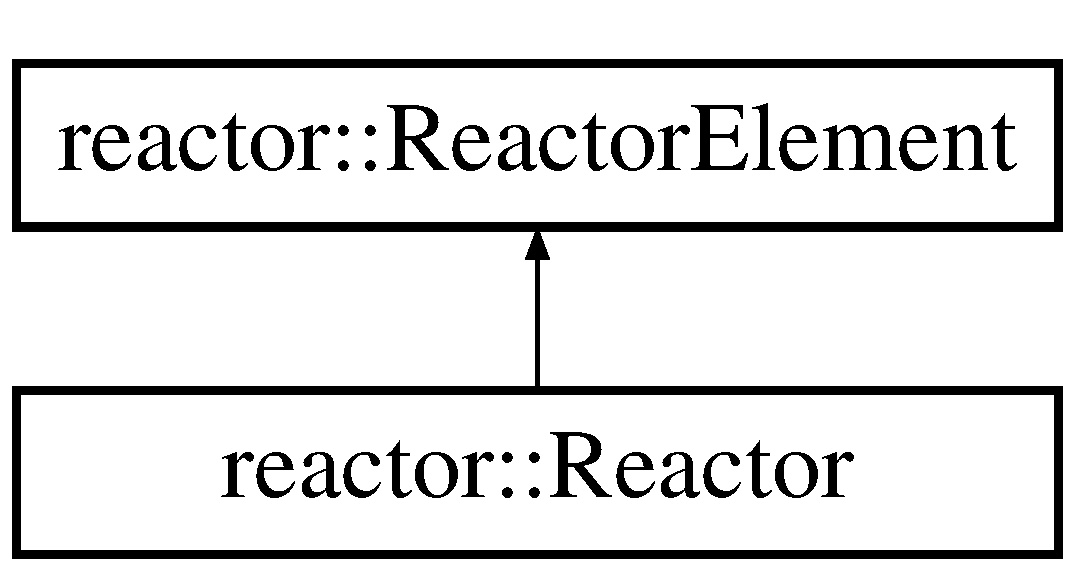
\includegraphics[height=2.000000cm]{classreactor_1_1Reactor}
\end{center}
\end{figure}
\subsection*{Public Member Functions}
\begin{DoxyCompactItemize}
\item 
\hyperlink{classreactor_1_1Reactor_a277765a261141f60ea6e8565533eb71c}{Reactor} (const std\+::string \&\hyperlink{classreactor_1_1ReactorElement_a99579f61dbaf5d5d98aebfe26eb8bf77}{name}, \hyperlink{classreactor_1_1Reactor}{Reactor} $\ast$\hyperlink{classreactor_1_1ReactorElement_a25bf298de879a82eefc1ba426be05812}{container})
\item 
\hyperlink{classreactor_1_1Reactor_af00ec5a8d0efcca675fc06d474181371}{Reactor} (const std\+::string \&\hyperlink{classreactor_1_1ReactorElement_a99579f61dbaf5d5d98aebfe26eb8bf77}{name}, \hyperlink{classreactor_1_1Environment}{Environment} $\ast$\hyperlink{classreactor_1_1ReactorElement_a895b09f977450723c59b67b41e643db8}{environment})
\item 
virtual \hyperlink{classreactor_1_1Reactor_a71a86bb46592e350cf173db091be6d50}{$\sim$\+Reactor} ()
\item 
const auto \& \hyperlink{classreactor_1_1Reactor_a6d4a4847eaf1da2ee81d1bf43ace739f}{actions} () const
\item 
const auto \& \hyperlink{classreactor_1_1Reactor_a9907a15d57a068a9785f1f5e74d0802a}{inputs} () const
\item 
const auto \& \hyperlink{classreactor_1_1Reactor_a6ee91ecde81bbffbb04773f1ae9b97dd}{outputs} () const
\item 
const auto \& \hyperlink{classreactor_1_1Reactor_a8667762f07039e52bfa7925a2a0fefc4}{reactions} () const
\item 
const auto \& \hyperlink{classreactor_1_1Reactor_ac69d7467dc9ec3db24a0c71e249d7eba}{reactors} () const
\item 
void \hyperlink{classreactor_1_1Reactor_ad254458867114f09a72e1e285ffc03d2}{startup} () override final
\item 
void \hyperlink{classreactor_1_1Reactor_ac65caf31e633bd76c45c794072afb56e}{shutdown} () override final
\item 
virtual void \hyperlink{classreactor_1_1Reactor_ac9d30ad0bc15043f154a59a4a390ab9f}{assemble} ()=0
\item 
\hyperlink{namespacereactor_ad950f8d1a46612500286a4af0f167080}{Time\+Point} \hyperlink{classreactor_1_1Reactor_abfdf519fd67c4fc13debc60dbc68bec3}{get\+\_\+physical\+\_\+time} () const
\item 
\hyperlink{namespacereactor_ad950f8d1a46612500286a4af0f167080}{Time\+Point} \hyperlink{classreactor_1_1Reactor_ae3b8bb1187b16901c8a140090579e6c9}{get\+\_\+logical\+\_\+time} () const
\item 
\hyperlink{namespacereactor_aa8375b807a80703545664096c5b5b779}{Duration} \hyperlink{classreactor_1_1Reactor_a4983e0e04f14212630b0a7da1f463239}{get\+\_\+elapsed\+\_\+logical\+\_\+time} () const
\item 
\hyperlink{namespacereactor_aa8375b807a80703545664096c5b5b779}{Duration} \hyperlink{classreactor_1_1Reactor_a206bd63d5ad7c2c39a89d9220f0acbbc}{get\+\_\+elapsed\+\_\+physical\+\_\+time} () const
\end{DoxyCompactItemize}
\subsection*{Public Attributes}
\begin{DoxyCompactItemize}
\item 
friend \hyperlink{classreactor_1_1Reactor_abd595c37f2e89b0bd53db2c0f18b1ad7}{Reactor\+Element}
\end{DoxyCompactItemize}
\subsection*{Private Member Functions}
\begin{DoxyCompactItemize}
\item 
void \hyperlink{classreactor_1_1Reactor_af03410009a1cac736179774282212219}{register\+\_\+action} (\hyperlink{classreactor_1_1BaseAction}{Base\+Action} $\ast$action)
\item 
void \hyperlink{classreactor_1_1Reactor_a026ca6574effbb38c4769c10efaef06d}{register\+\_\+port} (\hyperlink{classreactor_1_1BasePort}{Base\+Port} $\ast$port)
\item 
void \hyperlink{classreactor_1_1Reactor_a728acca5f61851ae9252df17e4b5e0ad}{register\+\_\+reaction} (\hyperlink{classreactor_1_1Reaction}{Reaction} $\ast$reaction)
\item 
void \hyperlink{classreactor_1_1Reactor_a120b7977b590c87b94066ff87c233650}{register\+\_\+reactor} (\hyperlink{classreactor_1_1Reactor}{Reactor} $\ast$reactor)
\end{DoxyCompactItemize}
\subsection*{Private Attributes}
\begin{DoxyCompactItemize}
\item 
std\+::set$<$ \hyperlink{classreactor_1_1BaseAction}{Base\+Action} $\ast$ $>$ \hyperlink{classreactor_1_1Reactor_a08956f27d0316095058663a1e234854c}{\+\_\+actions}
\item 
std\+::set$<$ \hyperlink{classreactor_1_1BasePort}{Base\+Port} $\ast$ $>$ \hyperlink{classreactor_1_1Reactor_a58b3ea8a7be4ff65de173fc8df01c8b1}{\+\_\+inputs}
\item 
std\+::set$<$ \hyperlink{classreactor_1_1BasePort}{Base\+Port} $\ast$ $>$ \hyperlink{classreactor_1_1Reactor_a925d1c0f776a963e9aac01084bdaedc2}{\+\_\+outputs}
\item 
std\+::set$<$ \hyperlink{classreactor_1_1Reaction}{Reaction} $\ast$ $>$ \hyperlink{classreactor_1_1Reactor_a894dedef16b5d6e927eecc223b0748ba}{\+\_\+reactions}
\item 
std\+::set$<$ \hyperlink{classreactor_1_1Reactor}{Reactor} $\ast$ $>$ \hyperlink{classreactor_1_1Reactor_aac609122effff608df6b5f3e5a1dc05b}{\+\_\+reactors}
\end{DoxyCompactItemize}
\subsection*{Additional Inherited Members}


\subsection{Constructor \& Destructor Documentation}
\mbox{\Hypertarget{classreactor_1_1Reactor_a277765a261141f60ea6e8565533eb71c}\label{classreactor_1_1Reactor_a277765a261141f60ea6e8565533eb71c}} 
\index{reactor\+::\+Reactor@{reactor\+::\+Reactor}!Reactor@{Reactor}}
\index{Reactor@{Reactor}!reactor\+::\+Reactor@{reactor\+::\+Reactor}}
\subsubsection{\texorpdfstring{Reactor()}{Reactor()}\hspace{0.1cm}{\footnotesize\ttfamily [1/2]}}
{\footnotesize\ttfamily reactor\+::\+Reactor\+::\+Reactor (\begin{DoxyParamCaption}\item[{const std\+::string \&}]{name,  }\item[{\hyperlink{classreactor_1_1Reactor}{Reactor} $\ast$}]{container }\end{DoxyParamCaption})}

\mbox{\Hypertarget{classreactor_1_1Reactor_af00ec5a8d0efcca675fc06d474181371}\label{classreactor_1_1Reactor_af00ec5a8d0efcca675fc06d474181371}} 
\index{reactor\+::\+Reactor@{reactor\+::\+Reactor}!Reactor@{Reactor}}
\index{Reactor@{Reactor}!reactor\+::\+Reactor@{reactor\+::\+Reactor}}
\subsubsection{\texorpdfstring{Reactor()}{Reactor()}\hspace{0.1cm}{\footnotesize\ttfamily [2/2]}}
{\footnotesize\ttfamily reactor\+::\+Reactor\+::\+Reactor (\begin{DoxyParamCaption}\item[{const std\+::string \&}]{name,  }\item[{\hyperlink{classreactor_1_1Environment}{Environment} $\ast$}]{environment }\end{DoxyParamCaption})}

\mbox{\Hypertarget{classreactor_1_1Reactor_a71a86bb46592e350cf173db091be6d50}\label{classreactor_1_1Reactor_a71a86bb46592e350cf173db091be6d50}} 
\index{reactor\+::\+Reactor@{reactor\+::\+Reactor}!````~Reactor@{$\sim$\+Reactor}}
\index{````~Reactor@{$\sim$\+Reactor}!reactor\+::\+Reactor@{reactor\+::\+Reactor}}
\subsubsection{\texorpdfstring{$\sim$\+Reactor()}{~Reactor()}}
{\footnotesize\ttfamily virtual reactor\+::\+Reactor\+::$\sim$\+Reactor (\begin{DoxyParamCaption}{ }\end{DoxyParamCaption})\hspace{0.3cm}{\ttfamily [inline]}, {\ttfamily [virtual]}}



\subsection{Member Function Documentation}
\mbox{\Hypertarget{classreactor_1_1Reactor_a6d4a4847eaf1da2ee81d1bf43ace739f}\label{classreactor_1_1Reactor_a6d4a4847eaf1da2ee81d1bf43ace739f}} 
\index{reactor\+::\+Reactor@{reactor\+::\+Reactor}!actions@{actions}}
\index{actions@{actions}!reactor\+::\+Reactor@{reactor\+::\+Reactor}}
\subsubsection{\texorpdfstring{actions()}{actions()}}
{\footnotesize\ttfamily const auto\& reactor\+::\+Reactor\+::actions (\begin{DoxyParamCaption}{ }\end{DoxyParamCaption}) const\hspace{0.3cm}{\ttfamily [inline]}}

\mbox{\Hypertarget{classreactor_1_1Reactor_ac9d30ad0bc15043f154a59a4a390ab9f}\label{classreactor_1_1Reactor_ac9d30ad0bc15043f154a59a4a390ab9f}} 
\index{reactor\+::\+Reactor@{reactor\+::\+Reactor}!assemble@{assemble}}
\index{assemble@{assemble}!reactor\+::\+Reactor@{reactor\+::\+Reactor}}
\subsubsection{\texorpdfstring{assemble()}{assemble()}}
{\footnotesize\ttfamily virtual void reactor\+::\+Reactor\+::assemble (\begin{DoxyParamCaption}{ }\end{DoxyParamCaption})\hspace{0.3cm}{\ttfamily [pure virtual]}}

\mbox{\Hypertarget{classreactor_1_1Reactor_a4983e0e04f14212630b0a7da1f463239}\label{classreactor_1_1Reactor_a4983e0e04f14212630b0a7da1f463239}} 
\index{reactor\+::\+Reactor@{reactor\+::\+Reactor}!get\+\_\+elapsed\+\_\+logical\+\_\+time@{get\+\_\+elapsed\+\_\+logical\+\_\+time}}
\index{get\+\_\+elapsed\+\_\+logical\+\_\+time@{get\+\_\+elapsed\+\_\+logical\+\_\+time}!reactor\+::\+Reactor@{reactor\+::\+Reactor}}
\subsubsection{\texorpdfstring{get\+\_\+elapsed\+\_\+logical\+\_\+time()}{get\_elapsed\_logical\_time()}}
{\footnotesize\ttfamily \hyperlink{namespacereactor_aa8375b807a80703545664096c5b5b779}{Duration} reactor\+::\+Reactor\+::get\+\_\+elapsed\+\_\+logical\+\_\+time (\begin{DoxyParamCaption}{ }\end{DoxyParamCaption}) const}

\mbox{\Hypertarget{classreactor_1_1Reactor_a206bd63d5ad7c2c39a89d9220f0acbbc}\label{classreactor_1_1Reactor_a206bd63d5ad7c2c39a89d9220f0acbbc}} 
\index{reactor\+::\+Reactor@{reactor\+::\+Reactor}!get\+\_\+elapsed\+\_\+physical\+\_\+time@{get\+\_\+elapsed\+\_\+physical\+\_\+time}}
\index{get\+\_\+elapsed\+\_\+physical\+\_\+time@{get\+\_\+elapsed\+\_\+physical\+\_\+time}!reactor\+::\+Reactor@{reactor\+::\+Reactor}}
\subsubsection{\texorpdfstring{get\+\_\+elapsed\+\_\+physical\+\_\+time()}{get\_elapsed\_physical\_time()}}
{\footnotesize\ttfamily \hyperlink{namespacereactor_aa8375b807a80703545664096c5b5b779}{Duration} reactor\+::\+Reactor\+::get\+\_\+elapsed\+\_\+physical\+\_\+time (\begin{DoxyParamCaption}{ }\end{DoxyParamCaption}) const}

\mbox{\Hypertarget{classreactor_1_1Reactor_ae3b8bb1187b16901c8a140090579e6c9}\label{classreactor_1_1Reactor_ae3b8bb1187b16901c8a140090579e6c9}} 
\index{reactor\+::\+Reactor@{reactor\+::\+Reactor}!get\+\_\+logical\+\_\+time@{get\+\_\+logical\+\_\+time}}
\index{get\+\_\+logical\+\_\+time@{get\+\_\+logical\+\_\+time}!reactor\+::\+Reactor@{reactor\+::\+Reactor}}
\subsubsection{\texorpdfstring{get\+\_\+logical\+\_\+time()}{get\_logical\_time()}}
{\footnotesize\ttfamily \hyperlink{namespacereactor_ad950f8d1a46612500286a4af0f167080}{Time\+Point} reactor\+::\+Reactor\+::get\+\_\+logical\+\_\+time (\begin{DoxyParamCaption}{ }\end{DoxyParamCaption}) const}

\mbox{\Hypertarget{classreactor_1_1Reactor_abfdf519fd67c4fc13debc60dbc68bec3}\label{classreactor_1_1Reactor_abfdf519fd67c4fc13debc60dbc68bec3}} 
\index{reactor\+::\+Reactor@{reactor\+::\+Reactor}!get\+\_\+physical\+\_\+time@{get\+\_\+physical\+\_\+time}}
\index{get\+\_\+physical\+\_\+time@{get\+\_\+physical\+\_\+time}!reactor\+::\+Reactor@{reactor\+::\+Reactor}}
\subsubsection{\texorpdfstring{get\+\_\+physical\+\_\+time()}{get\_physical\_time()}}
{\footnotesize\ttfamily \hyperlink{namespacereactor_ad950f8d1a46612500286a4af0f167080}{Time\+Point} reactor\+::\+Reactor\+::get\+\_\+physical\+\_\+time (\begin{DoxyParamCaption}{ }\end{DoxyParamCaption}) const}

\mbox{\Hypertarget{classreactor_1_1Reactor_a9907a15d57a068a9785f1f5e74d0802a}\label{classreactor_1_1Reactor_a9907a15d57a068a9785f1f5e74d0802a}} 
\index{reactor\+::\+Reactor@{reactor\+::\+Reactor}!inputs@{inputs}}
\index{inputs@{inputs}!reactor\+::\+Reactor@{reactor\+::\+Reactor}}
\subsubsection{\texorpdfstring{inputs()}{inputs()}}
{\footnotesize\ttfamily const auto\& reactor\+::\+Reactor\+::inputs (\begin{DoxyParamCaption}{ }\end{DoxyParamCaption}) const\hspace{0.3cm}{\ttfamily [inline]}}

\mbox{\Hypertarget{classreactor_1_1Reactor_a6ee91ecde81bbffbb04773f1ae9b97dd}\label{classreactor_1_1Reactor_a6ee91ecde81bbffbb04773f1ae9b97dd}} 
\index{reactor\+::\+Reactor@{reactor\+::\+Reactor}!outputs@{outputs}}
\index{outputs@{outputs}!reactor\+::\+Reactor@{reactor\+::\+Reactor}}
\subsubsection{\texorpdfstring{outputs()}{outputs()}}
{\footnotesize\ttfamily const auto\& reactor\+::\+Reactor\+::outputs (\begin{DoxyParamCaption}{ }\end{DoxyParamCaption}) const\hspace{0.3cm}{\ttfamily [inline]}}

\mbox{\Hypertarget{classreactor_1_1Reactor_a8667762f07039e52bfa7925a2a0fefc4}\label{classreactor_1_1Reactor_a8667762f07039e52bfa7925a2a0fefc4}} 
\index{reactor\+::\+Reactor@{reactor\+::\+Reactor}!reactions@{reactions}}
\index{reactions@{reactions}!reactor\+::\+Reactor@{reactor\+::\+Reactor}}
\subsubsection{\texorpdfstring{reactions()}{reactions()}}
{\footnotesize\ttfamily const auto\& reactor\+::\+Reactor\+::reactions (\begin{DoxyParamCaption}{ }\end{DoxyParamCaption}) const\hspace{0.3cm}{\ttfamily [inline]}}

\mbox{\Hypertarget{classreactor_1_1Reactor_ac69d7467dc9ec3db24a0c71e249d7eba}\label{classreactor_1_1Reactor_ac69d7467dc9ec3db24a0c71e249d7eba}} 
\index{reactor\+::\+Reactor@{reactor\+::\+Reactor}!reactors@{reactors}}
\index{reactors@{reactors}!reactor\+::\+Reactor@{reactor\+::\+Reactor}}
\subsubsection{\texorpdfstring{reactors()}{reactors()}}
{\footnotesize\ttfamily const auto\& reactor\+::\+Reactor\+::reactors (\begin{DoxyParamCaption}{ }\end{DoxyParamCaption}) const\hspace{0.3cm}{\ttfamily [inline]}}

\mbox{\Hypertarget{classreactor_1_1Reactor_af03410009a1cac736179774282212219}\label{classreactor_1_1Reactor_af03410009a1cac736179774282212219}} 
\index{reactor\+::\+Reactor@{reactor\+::\+Reactor}!register\+\_\+action@{register\+\_\+action}}
\index{register\+\_\+action@{register\+\_\+action}!reactor\+::\+Reactor@{reactor\+::\+Reactor}}
\subsubsection{\texorpdfstring{register\+\_\+action()}{register\_action()}}
{\footnotesize\ttfamily void reactor\+::\+Reactor\+::register\+\_\+action (\begin{DoxyParamCaption}\item[{\hyperlink{classreactor_1_1BaseAction}{Base\+Action} $\ast$}]{action }\end{DoxyParamCaption})\hspace{0.3cm}{\ttfamily [private]}}

\mbox{\Hypertarget{classreactor_1_1Reactor_a026ca6574effbb38c4769c10efaef06d}\label{classreactor_1_1Reactor_a026ca6574effbb38c4769c10efaef06d}} 
\index{reactor\+::\+Reactor@{reactor\+::\+Reactor}!register\+\_\+port@{register\+\_\+port}}
\index{register\+\_\+port@{register\+\_\+port}!reactor\+::\+Reactor@{reactor\+::\+Reactor}}
\subsubsection{\texorpdfstring{register\+\_\+port()}{register\_port()}}
{\footnotesize\ttfamily void reactor\+::\+Reactor\+::register\+\_\+port (\begin{DoxyParamCaption}\item[{\hyperlink{classreactor_1_1BasePort}{Base\+Port} $\ast$}]{port }\end{DoxyParamCaption})\hspace{0.3cm}{\ttfamily [private]}}

\mbox{\Hypertarget{classreactor_1_1Reactor_a728acca5f61851ae9252df17e4b5e0ad}\label{classreactor_1_1Reactor_a728acca5f61851ae9252df17e4b5e0ad}} 
\index{reactor\+::\+Reactor@{reactor\+::\+Reactor}!register\+\_\+reaction@{register\+\_\+reaction}}
\index{register\+\_\+reaction@{register\+\_\+reaction}!reactor\+::\+Reactor@{reactor\+::\+Reactor}}
\subsubsection{\texorpdfstring{register\+\_\+reaction()}{register\_reaction()}}
{\footnotesize\ttfamily void reactor\+::\+Reactor\+::register\+\_\+reaction (\begin{DoxyParamCaption}\item[{\hyperlink{classreactor_1_1Reaction}{Reaction} $\ast$}]{reaction }\end{DoxyParamCaption})\hspace{0.3cm}{\ttfamily [private]}}

\mbox{\Hypertarget{classreactor_1_1Reactor_a120b7977b590c87b94066ff87c233650}\label{classreactor_1_1Reactor_a120b7977b590c87b94066ff87c233650}} 
\index{reactor\+::\+Reactor@{reactor\+::\+Reactor}!register\+\_\+reactor@{register\+\_\+reactor}}
\index{register\+\_\+reactor@{register\+\_\+reactor}!reactor\+::\+Reactor@{reactor\+::\+Reactor}}
\subsubsection{\texorpdfstring{register\+\_\+reactor()}{register\_reactor()}}
{\footnotesize\ttfamily void reactor\+::\+Reactor\+::register\+\_\+reactor (\begin{DoxyParamCaption}\item[{\hyperlink{classreactor_1_1Reactor}{Reactor} $\ast$}]{reactor }\end{DoxyParamCaption})\hspace{0.3cm}{\ttfamily [private]}}

\mbox{\Hypertarget{classreactor_1_1Reactor_ac65caf31e633bd76c45c794072afb56e}\label{classreactor_1_1Reactor_ac65caf31e633bd76c45c794072afb56e}} 
\index{reactor\+::\+Reactor@{reactor\+::\+Reactor}!shutdown@{shutdown}}
\index{shutdown@{shutdown}!reactor\+::\+Reactor@{reactor\+::\+Reactor}}
\subsubsection{\texorpdfstring{shutdown()}{shutdown()}}
{\footnotesize\ttfamily void reactor\+::\+Reactor\+::shutdown (\begin{DoxyParamCaption}{ }\end{DoxyParamCaption})\hspace{0.3cm}{\ttfamily [final]}, {\ttfamily [override]}, {\ttfamily [virtual]}}



Implements \hyperlink{classreactor_1_1ReactorElement_a8fce084bef582156979ebba56737e907}{reactor\+::\+Reactor\+Element}.

\mbox{\Hypertarget{classreactor_1_1Reactor_ad254458867114f09a72e1e285ffc03d2}\label{classreactor_1_1Reactor_ad254458867114f09a72e1e285ffc03d2}} 
\index{reactor\+::\+Reactor@{reactor\+::\+Reactor}!startup@{startup}}
\index{startup@{startup}!reactor\+::\+Reactor@{reactor\+::\+Reactor}}
\subsubsection{\texorpdfstring{startup()}{startup()}}
{\footnotesize\ttfamily void reactor\+::\+Reactor\+::startup (\begin{DoxyParamCaption}{ }\end{DoxyParamCaption})\hspace{0.3cm}{\ttfamily [final]}, {\ttfamily [override]}, {\ttfamily [virtual]}}



Implements \hyperlink{classreactor_1_1ReactorElement_a8cb574cb20ff963903ad905fb0a157e3}{reactor\+::\+Reactor\+Element}.



\subsection{Member Data Documentation}
\mbox{\Hypertarget{classreactor_1_1Reactor_a08956f27d0316095058663a1e234854c}\label{classreactor_1_1Reactor_a08956f27d0316095058663a1e234854c}} 
\index{reactor\+::\+Reactor@{reactor\+::\+Reactor}!\+\_\+actions@{\+\_\+actions}}
\index{\+\_\+actions@{\+\_\+actions}!reactor\+::\+Reactor@{reactor\+::\+Reactor}}
\subsubsection{\texorpdfstring{\+\_\+actions}{\_actions}}
{\footnotesize\ttfamily std\+::set$<$\hyperlink{classreactor_1_1BaseAction}{Base\+Action}$\ast$$>$ reactor\+::\+Reactor\+::\+\_\+actions\hspace{0.3cm}{\ttfamily [private]}}

\mbox{\Hypertarget{classreactor_1_1Reactor_a58b3ea8a7be4ff65de173fc8df01c8b1}\label{classreactor_1_1Reactor_a58b3ea8a7be4ff65de173fc8df01c8b1}} 
\index{reactor\+::\+Reactor@{reactor\+::\+Reactor}!\+\_\+inputs@{\+\_\+inputs}}
\index{\+\_\+inputs@{\+\_\+inputs}!reactor\+::\+Reactor@{reactor\+::\+Reactor}}
\subsubsection{\texorpdfstring{\+\_\+inputs}{\_inputs}}
{\footnotesize\ttfamily std\+::set$<$\hyperlink{classreactor_1_1BasePort}{Base\+Port}$\ast$$>$ reactor\+::\+Reactor\+::\+\_\+inputs\hspace{0.3cm}{\ttfamily [private]}}

\mbox{\Hypertarget{classreactor_1_1Reactor_a925d1c0f776a963e9aac01084bdaedc2}\label{classreactor_1_1Reactor_a925d1c0f776a963e9aac01084bdaedc2}} 
\index{reactor\+::\+Reactor@{reactor\+::\+Reactor}!\+\_\+outputs@{\+\_\+outputs}}
\index{\+\_\+outputs@{\+\_\+outputs}!reactor\+::\+Reactor@{reactor\+::\+Reactor}}
\subsubsection{\texorpdfstring{\+\_\+outputs}{\_outputs}}
{\footnotesize\ttfamily std\+::set$<$\hyperlink{classreactor_1_1BasePort}{Base\+Port}$\ast$$>$ reactor\+::\+Reactor\+::\+\_\+outputs\hspace{0.3cm}{\ttfamily [private]}}

\mbox{\Hypertarget{classreactor_1_1Reactor_a894dedef16b5d6e927eecc223b0748ba}\label{classreactor_1_1Reactor_a894dedef16b5d6e927eecc223b0748ba}} 
\index{reactor\+::\+Reactor@{reactor\+::\+Reactor}!\+\_\+reactions@{\+\_\+reactions}}
\index{\+\_\+reactions@{\+\_\+reactions}!reactor\+::\+Reactor@{reactor\+::\+Reactor}}
\subsubsection{\texorpdfstring{\+\_\+reactions}{\_reactions}}
{\footnotesize\ttfamily std\+::set$<$\hyperlink{classreactor_1_1Reaction}{Reaction}$\ast$$>$ reactor\+::\+Reactor\+::\+\_\+reactions\hspace{0.3cm}{\ttfamily [private]}}

\mbox{\Hypertarget{classreactor_1_1Reactor_aac609122effff608df6b5f3e5a1dc05b}\label{classreactor_1_1Reactor_aac609122effff608df6b5f3e5a1dc05b}} 
\index{reactor\+::\+Reactor@{reactor\+::\+Reactor}!\+\_\+reactors@{\+\_\+reactors}}
\index{\+\_\+reactors@{\+\_\+reactors}!reactor\+::\+Reactor@{reactor\+::\+Reactor}}
\subsubsection{\texorpdfstring{\+\_\+reactors}{\_reactors}}
{\footnotesize\ttfamily std\+::set$<$\hyperlink{classreactor_1_1Reactor}{Reactor}$\ast$$>$ reactor\+::\+Reactor\+::\+\_\+reactors\hspace{0.3cm}{\ttfamily [private]}}

\mbox{\Hypertarget{classreactor_1_1Reactor_abd595c37f2e89b0bd53db2c0f18b1ad7}\label{classreactor_1_1Reactor_abd595c37f2e89b0bd53db2c0f18b1ad7}} 
\index{reactor\+::\+Reactor@{reactor\+::\+Reactor}!Reactor\+Element@{Reactor\+Element}}
\index{Reactor\+Element@{Reactor\+Element}!reactor\+::\+Reactor@{reactor\+::\+Reactor}}
\subsubsection{\texorpdfstring{Reactor\+Element}{ReactorElement}}
{\footnotesize\ttfamily friend reactor\+::\+Reactor\+::\+Reactor\+Element}



The documentation for this class was generated from the following files\+:\begin{DoxyCompactItemize}
\item 
/home/runner/work/reactor-\/cpp/reactor-\/cpp/include/reactor-\/cpp/\hyperlink{reactor_8hh}{reactor.\+hh}\item 
/home/runner/work/reactor-\/cpp/reactor-\/cpp/lib/\hyperlink{reactor_8cc}{reactor.\+cc}\end{DoxyCompactItemize}

\hypertarget{classreactor_1_1ReactorElement}{}\section{reactor\+:\+:Reactor\+Element Class Reference}
\label{classreactor_1_1ReactorElement}\index{reactor\+::\+Reactor\+Element@{reactor\+::\+Reactor\+Element}}


{\ttfamily \#include $<$reactor.\+hh$>$}

Inheritance diagram for reactor\+:\+:Reactor\+Element\+:\begin{figure}[H]
\begin{center}
\leavevmode
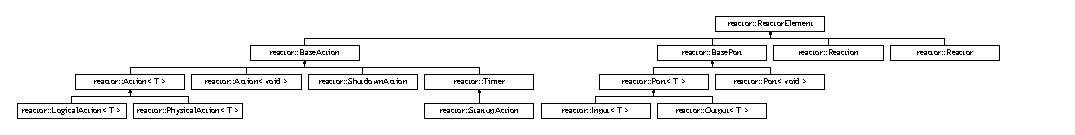
\includegraphics[height=1.367521cm]{classreactor_1_1ReactorElement}
\end{center}
\end{figure}
\subsection*{Public Types}
\begin{DoxyCompactItemize}
\item 
enum \hyperlink{classreactor_1_1ReactorElement_a9291659e2893372cfea42ffccfd487b2}{Type} \{ \hyperlink{classreactor_1_1ReactorElement_a9291659e2893372cfea42ffccfd487b2a004bf6c9a40003140292e97330236c53}{Type\+::\+Action}, 
\hyperlink{classreactor_1_1ReactorElement_a9291659e2893372cfea42ffccfd487b2a60aaf44d4b562252c04db7f98497e9aa}{Type\+::\+Port}, 
\hyperlink{classreactor_1_1ReactorElement_a9291659e2893372cfea42ffccfd487b2aa87198fb6a6b4fe0b70c03fc2a43a8f4}{Type\+::\+Reaction}, 
\hyperlink{classreactor_1_1ReactorElement_a9291659e2893372cfea42ffccfd487b2a1436185f7342e0210be86e7e17963250}{Type\+::\+Reactor}
 \}
\end{DoxyCompactItemize}
\subsection*{Public Member Functions}
\begin{DoxyCompactItemize}
\item 
\hyperlink{classreactor_1_1ReactorElement_aebc8c1cabcadca08400284fdb05ce746}{Reactor\+Element} (const std\+::string \&\hyperlink{classreactor_1_1ReactorElement_a99579f61dbaf5d5d98aebfe26eb8bf77}{name}, \hyperlink{classreactor_1_1ReactorElement_a9291659e2893372cfea42ffccfd487b2}{Type} type, \hyperlink{classreactor_1_1Reactor}{Reactor} $\ast$\hyperlink{classreactor_1_1ReactorElement_a25bf298de879a82eefc1ba426be05812}{container})
\item 
\hyperlink{classreactor_1_1ReactorElement_ac5f85a8322de3fad7191a8f749b507fd}{Reactor\+Element} (const std\+::string \&\hyperlink{classreactor_1_1ReactorElement_a99579f61dbaf5d5d98aebfe26eb8bf77}{name}, \hyperlink{classreactor_1_1ReactorElement_a9291659e2893372cfea42ffccfd487b2}{Type} type, \hyperlink{classreactor_1_1Environment}{Environment} $\ast$\hyperlink{classreactor_1_1ReactorElement_a895b09f977450723c59b67b41e643db8}{environment})
\item 
virtual \hyperlink{classreactor_1_1ReactorElement_ac9075040ad83b1945f75f3065c0405fa}{$\sim$\+Reactor\+Element} ()
\item 
\hyperlink{classreactor_1_1ReactorElement_aa975574e21f5f7a4bb761f04ed57dfa4}{Reactor\+Element} (const \hyperlink{classreactor_1_1ReactorElement}{Reactor\+Element} \&)=delete
\item 
\hyperlink{classreactor_1_1ReactorElement_a2ba6e1e309233db7cfc124563f9f8f9f}{Reactor\+Element} (\hyperlink{classreactor_1_1ReactorElement}{Reactor\+Element} \&\&)=delete
\item 
\hyperlink{classreactor_1_1Reactor}{Reactor} $\ast$ \hyperlink{classreactor_1_1ReactorElement_a25bf298de879a82eefc1ba426be05812}{container} () const
\item 
const std\+::string \& \hyperlink{classreactor_1_1ReactorElement_a99579f61dbaf5d5d98aebfe26eb8bf77}{name} () const
\item 
const std\+::string \& \hyperlink{classreactor_1_1ReactorElement_af57b89113cd189208ea95668ad5bd141}{fqn} () const
\item 
\hyperlink{classreactor_1_1Environment}{Environment} $\ast$ \hyperlink{classreactor_1_1ReactorElement_a895b09f977450723c59b67b41e643db8}{environment} () const
\item 
bool \hyperlink{classreactor_1_1ReactorElement_a29c516a59fd1ccc43fa0023c550b6964}{is\+\_\+top\+\_\+level} () const
\item 
virtual void \hyperlink{classreactor_1_1ReactorElement_a8cb574cb20ff963903ad905fb0a157e3}{startup} ()=0
\item 
virtual void \hyperlink{classreactor_1_1ReactorElement_a8fce084bef582156979ebba56737e907}{shutdown} ()=0
\end{DoxyCompactItemize}
\subsection*{Private Member Functions}
\begin{DoxyCompactItemize}
\item 
std\+::stringstream \& \hyperlink{classreactor_1_1ReactorElement_a8adcf9dcdd516372915527106a263273}{fqn\+\_\+detail} (std\+::stringstream \&ss) const
\end{DoxyCompactItemize}
\subsection*{Private Attributes}
\begin{DoxyCompactItemize}
\item 
const std\+::string \hyperlink{classreactor_1_1ReactorElement_a228fa190e96b14e7ea08bb18e7a95ae7}{\+\_\+name}
\item 
std\+::string \hyperlink{classreactor_1_1ReactorElement_a4c82246281c31e97b3d18c25670f8072}{\+\_\+fqn}
\item 
\hyperlink{classreactor_1_1Reactor}{Reactor} $\ast$const \hyperlink{classreactor_1_1ReactorElement_a247c6863a035b15938b4bbc0a07b664d}{\+\_\+container}
\begin{DoxyCompactList}\small\item\em The reactor owning this element. \end{DoxyCompactList}\item 
\hyperlink{classreactor_1_1Environment}{Environment} $\ast$ \hyperlink{classreactor_1_1ReactorElement_a07b433591c3e20916b46ecd6ef3c2bf8}{\+\_\+environment}
\end{DoxyCompactItemize}


\subsection{Member Enumeration Documentation}
\mbox{\Hypertarget{classreactor_1_1ReactorElement_a9291659e2893372cfea42ffccfd487b2}\label{classreactor_1_1ReactorElement_a9291659e2893372cfea42ffccfd487b2}} 
\index{reactor\+::\+Reactor\+Element@{reactor\+::\+Reactor\+Element}!Type@{Type}}
\index{Type@{Type}!reactor\+::\+Reactor\+Element@{reactor\+::\+Reactor\+Element}}
\subsubsection{\texorpdfstring{Type}{Type}}
{\footnotesize\ttfamily enum \hyperlink{classreactor_1_1ReactorElement_a9291659e2893372cfea42ffccfd487b2}{reactor\+::\+Reactor\+Element\+::\+Type}\hspace{0.3cm}{\ttfamily [strong]}}

\begin{DoxyEnumFields}{Enumerator}
\raisebox{\heightof{T}}[0pt][0pt]{\index{Action@{Action}!reactor\+::\+Reactor\+Element@{reactor\+::\+Reactor\+Element}}\index{reactor\+::\+Reactor\+Element@{reactor\+::\+Reactor\+Element}!Action@{Action}}}\mbox{\Hypertarget{classreactor_1_1ReactorElement_a9291659e2893372cfea42ffccfd487b2a004bf6c9a40003140292e97330236c53}\label{classreactor_1_1ReactorElement_a9291659e2893372cfea42ffccfd487b2a004bf6c9a40003140292e97330236c53}} 
Action&\\
\hline

\raisebox{\heightof{T}}[0pt][0pt]{\index{Port@{Port}!reactor\+::\+Reactor\+Element@{reactor\+::\+Reactor\+Element}}\index{reactor\+::\+Reactor\+Element@{reactor\+::\+Reactor\+Element}!Port@{Port}}}\mbox{\Hypertarget{classreactor_1_1ReactorElement_a9291659e2893372cfea42ffccfd487b2a60aaf44d4b562252c04db7f98497e9aa}\label{classreactor_1_1ReactorElement_a9291659e2893372cfea42ffccfd487b2a60aaf44d4b562252c04db7f98497e9aa}} 
Port&\\
\hline

\raisebox{\heightof{T}}[0pt][0pt]{\index{Reaction@{Reaction}!reactor\+::\+Reactor\+Element@{reactor\+::\+Reactor\+Element}}\index{reactor\+::\+Reactor\+Element@{reactor\+::\+Reactor\+Element}!Reaction@{Reaction}}}\mbox{\Hypertarget{classreactor_1_1ReactorElement_a9291659e2893372cfea42ffccfd487b2aa87198fb6a6b4fe0b70c03fc2a43a8f4}\label{classreactor_1_1ReactorElement_a9291659e2893372cfea42ffccfd487b2aa87198fb6a6b4fe0b70c03fc2a43a8f4}} 
Reaction&\\
\hline

\raisebox{\heightof{T}}[0pt][0pt]{\index{Reactor@{Reactor}!reactor\+::\+Reactor\+Element@{reactor\+::\+Reactor\+Element}}\index{reactor\+::\+Reactor\+Element@{reactor\+::\+Reactor\+Element}!Reactor@{Reactor}}}\mbox{\Hypertarget{classreactor_1_1ReactorElement_a9291659e2893372cfea42ffccfd487b2a1436185f7342e0210be86e7e17963250}\label{classreactor_1_1ReactorElement_a9291659e2893372cfea42ffccfd487b2a1436185f7342e0210be86e7e17963250}} 
Reactor&\\
\hline

\end{DoxyEnumFields}


\subsection{Constructor \& Destructor Documentation}
\mbox{\Hypertarget{classreactor_1_1ReactorElement_aebc8c1cabcadca08400284fdb05ce746}\label{classreactor_1_1ReactorElement_aebc8c1cabcadca08400284fdb05ce746}} 
\index{reactor\+::\+Reactor\+Element@{reactor\+::\+Reactor\+Element}!Reactor\+Element@{Reactor\+Element}}
\index{Reactor\+Element@{Reactor\+Element}!reactor\+::\+Reactor\+Element@{reactor\+::\+Reactor\+Element}}
\subsubsection{\texorpdfstring{Reactor\+Element()}{ReactorElement()}\hspace{0.1cm}{\footnotesize\ttfamily [1/4]}}
{\footnotesize\ttfamily reactor\+::\+Reactor\+Element\+::\+Reactor\+Element (\begin{DoxyParamCaption}\item[{const std\+::string \&}]{name,  }\item[{\hyperlink{classreactor_1_1ReactorElement_a9291659e2893372cfea42ffccfd487b2}{Reactor\+Element\+::\+Type}}]{type,  }\item[{\hyperlink{classreactor_1_1Reactor}{Reactor} $\ast$}]{container }\end{DoxyParamCaption})}

\mbox{\Hypertarget{classreactor_1_1ReactorElement_ac5f85a8322de3fad7191a8f749b507fd}\label{classreactor_1_1ReactorElement_ac5f85a8322de3fad7191a8f749b507fd}} 
\index{reactor\+::\+Reactor\+Element@{reactor\+::\+Reactor\+Element}!Reactor\+Element@{Reactor\+Element}}
\index{Reactor\+Element@{Reactor\+Element}!reactor\+::\+Reactor\+Element@{reactor\+::\+Reactor\+Element}}
\subsubsection{\texorpdfstring{Reactor\+Element()}{ReactorElement()}\hspace{0.1cm}{\footnotesize\ttfamily [2/4]}}
{\footnotesize\ttfamily reactor\+::\+Reactor\+Element\+::\+Reactor\+Element (\begin{DoxyParamCaption}\item[{const std\+::string \&}]{name,  }\item[{\hyperlink{classreactor_1_1ReactorElement_a9291659e2893372cfea42ffccfd487b2}{Reactor\+Element\+::\+Type}}]{type,  }\item[{\hyperlink{classreactor_1_1Environment}{Environment} $\ast$}]{environment }\end{DoxyParamCaption})}

\mbox{\Hypertarget{classreactor_1_1ReactorElement_ac9075040ad83b1945f75f3065c0405fa}\label{classreactor_1_1ReactorElement_ac9075040ad83b1945f75f3065c0405fa}} 
\index{reactor\+::\+Reactor\+Element@{reactor\+::\+Reactor\+Element}!````~Reactor\+Element@{$\sim$\+Reactor\+Element}}
\index{````~Reactor\+Element@{$\sim$\+Reactor\+Element}!reactor\+::\+Reactor\+Element@{reactor\+::\+Reactor\+Element}}
\subsubsection{\texorpdfstring{$\sim$\+Reactor\+Element()}{~ReactorElement()}}
{\footnotesize\ttfamily virtual reactor\+::\+Reactor\+Element\+::$\sim$\+Reactor\+Element (\begin{DoxyParamCaption}{ }\end{DoxyParamCaption})\hspace{0.3cm}{\ttfamily [inline]}, {\ttfamily [virtual]}}

\mbox{\Hypertarget{classreactor_1_1ReactorElement_aa975574e21f5f7a4bb761f04ed57dfa4}\label{classreactor_1_1ReactorElement_aa975574e21f5f7a4bb761f04ed57dfa4}} 
\index{reactor\+::\+Reactor\+Element@{reactor\+::\+Reactor\+Element}!Reactor\+Element@{Reactor\+Element}}
\index{Reactor\+Element@{Reactor\+Element}!reactor\+::\+Reactor\+Element@{reactor\+::\+Reactor\+Element}}
\subsubsection{\texorpdfstring{Reactor\+Element()}{ReactorElement()}\hspace{0.1cm}{\footnotesize\ttfamily [3/4]}}
{\footnotesize\ttfamily reactor\+::\+Reactor\+Element\+::\+Reactor\+Element (\begin{DoxyParamCaption}\item[{const \hyperlink{classreactor_1_1ReactorElement}{Reactor\+Element} \&}]{ }\end{DoxyParamCaption})\hspace{0.3cm}{\ttfamily [delete]}}

\mbox{\Hypertarget{classreactor_1_1ReactorElement_a2ba6e1e309233db7cfc124563f9f8f9f}\label{classreactor_1_1ReactorElement_a2ba6e1e309233db7cfc124563f9f8f9f}} 
\index{reactor\+::\+Reactor\+Element@{reactor\+::\+Reactor\+Element}!Reactor\+Element@{Reactor\+Element}}
\index{Reactor\+Element@{Reactor\+Element}!reactor\+::\+Reactor\+Element@{reactor\+::\+Reactor\+Element}}
\subsubsection{\texorpdfstring{Reactor\+Element()}{ReactorElement()}\hspace{0.1cm}{\footnotesize\ttfamily [4/4]}}
{\footnotesize\ttfamily reactor\+::\+Reactor\+Element\+::\+Reactor\+Element (\begin{DoxyParamCaption}\item[{\hyperlink{classreactor_1_1ReactorElement}{Reactor\+Element} \&\&}]{ }\end{DoxyParamCaption})\hspace{0.3cm}{\ttfamily [delete]}}



\subsection{Member Function Documentation}
\mbox{\Hypertarget{classreactor_1_1ReactorElement_a25bf298de879a82eefc1ba426be05812}\label{classreactor_1_1ReactorElement_a25bf298de879a82eefc1ba426be05812}} 
\index{reactor\+::\+Reactor\+Element@{reactor\+::\+Reactor\+Element}!container@{container}}
\index{container@{container}!reactor\+::\+Reactor\+Element@{reactor\+::\+Reactor\+Element}}
\subsubsection{\texorpdfstring{container()}{container()}}
{\footnotesize\ttfamily \hyperlink{classreactor_1_1Reactor}{Reactor}$\ast$ reactor\+::\+Reactor\+Element\+::container (\begin{DoxyParamCaption}{ }\end{DoxyParamCaption}) const\hspace{0.3cm}{\ttfamily [inline]}}

\mbox{\Hypertarget{classreactor_1_1ReactorElement_a895b09f977450723c59b67b41e643db8}\label{classreactor_1_1ReactorElement_a895b09f977450723c59b67b41e643db8}} 
\index{reactor\+::\+Reactor\+Element@{reactor\+::\+Reactor\+Element}!environment@{environment}}
\index{environment@{environment}!reactor\+::\+Reactor\+Element@{reactor\+::\+Reactor\+Element}}
\subsubsection{\texorpdfstring{environment()}{environment()}}
{\footnotesize\ttfamily \hyperlink{classreactor_1_1Environment}{Environment}$\ast$ reactor\+::\+Reactor\+Element\+::environment (\begin{DoxyParamCaption}{ }\end{DoxyParamCaption}) const\hspace{0.3cm}{\ttfamily [inline]}}

\mbox{\Hypertarget{classreactor_1_1ReactorElement_af57b89113cd189208ea95668ad5bd141}\label{classreactor_1_1ReactorElement_af57b89113cd189208ea95668ad5bd141}} 
\index{reactor\+::\+Reactor\+Element@{reactor\+::\+Reactor\+Element}!fqn@{fqn}}
\index{fqn@{fqn}!reactor\+::\+Reactor\+Element@{reactor\+::\+Reactor\+Element}}
\subsubsection{\texorpdfstring{fqn()}{fqn()}}
{\footnotesize\ttfamily const std\+::string\& reactor\+::\+Reactor\+Element\+::fqn (\begin{DoxyParamCaption}{ }\end{DoxyParamCaption}) const\hspace{0.3cm}{\ttfamily [inline]}}

\mbox{\Hypertarget{classreactor_1_1ReactorElement_a8adcf9dcdd516372915527106a263273}\label{classreactor_1_1ReactorElement_a8adcf9dcdd516372915527106a263273}} 
\index{reactor\+::\+Reactor\+Element@{reactor\+::\+Reactor\+Element}!fqn\+\_\+detail@{fqn\+\_\+detail}}
\index{fqn\+\_\+detail@{fqn\+\_\+detail}!reactor\+::\+Reactor\+Element@{reactor\+::\+Reactor\+Element}}
\subsubsection{\texorpdfstring{fqn\+\_\+detail()}{fqn\_detail()}}
{\footnotesize\ttfamily std\+::stringstream\& reactor\+::\+Reactor\+Element\+::fqn\+\_\+detail (\begin{DoxyParamCaption}\item[{std\+::stringstream \&}]{ss }\end{DoxyParamCaption}) const\hspace{0.3cm}{\ttfamily [private]}}

\mbox{\Hypertarget{classreactor_1_1ReactorElement_a29c516a59fd1ccc43fa0023c550b6964}\label{classreactor_1_1ReactorElement_a29c516a59fd1ccc43fa0023c550b6964}} 
\index{reactor\+::\+Reactor\+Element@{reactor\+::\+Reactor\+Element}!is\+\_\+top\+\_\+level@{is\+\_\+top\+\_\+level}}
\index{is\+\_\+top\+\_\+level@{is\+\_\+top\+\_\+level}!reactor\+::\+Reactor\+Element@{reactor\+::\+Reactor\+Element}}
\subsubsection{\texorpdfstring{is\+\_\+top\+\_\+level()}{is\_top\_level()}}
{\footnotesize\ttfamily bool reactor\+::\+Reactor\+Element\+::is\+\_\+top\+\_\+level (\begin{DoxyParamCaption}{ }\end{DoxyParamCaption}) const\hspace{0.3cm}{\ttfamily [inline]}}

\mbox{\Hypertarget{classreactor_1_1ReactorElement_a99579f61dbaf5d5d98aebfe26eb8bf77}\label{classreactor_1_1ReactorElement_a99579f61dbaf5d5d98aebfe26eb8bf77}} 
\index{reactor\+::\+Reactor\+Element@{reactor\+::\+Reactor\+Element}!name@{name}}
\index{name@{name}!reactor\+::\+Reactor\+Element@{reactor\+::\+Reactor\+Element}}
\subsubsection{\texorpdfstring{name()}{name()}}
{\footnotesize\ttfamily const std\+::string\& reactor\+::\+Reactor\+Element\+::name (\begin{DoxyParamCaption}{ }\end{DoxyParamCaption}) const\hspace{0.3cm}{\ttfamily [inline]}}

\mbox{\Hypertarget{classreactor_1_1ReactorElement_a8fce084bef582156979ebba56737e907}\label{classreactor_1_1ReactorElement_a8fce084bef582156979ebba56737e907}} 
\index{reactor\+::\+Reactor\+Element@{reactor\+::\+Reactor\+Element}!shutdown@{shutdown}}
\index{shutdown@{shutdown}!reactor\+::\+Reactor\+Element@{reactor\+::\+Reactor\+Element}}
\subsubsection{\texorpdfstring{shutdown()}{shutdown()}}
{\footnotesize\ttfamily virtual void reactor\+::\+Reactor\+Element\+::shutdown (\begin{DoxyParamCaption}{ }\end{DoxyParamCaption})\hspace{0.3cm}{\ttfamily [pure virtual]}}



Implemented in \hyperlink{classreactor_1_1ShutdownAction_a8950ffd9b67f4800b75a95af92c4fd2a}{reactor\+::\+Shutdown\+Action}, \hyperlink{classreactor_1_1Timer_a35f218aab3bf72b87cff4aa984dee991}{reactor\+::\+Timer}, \hyperlink{classreactor_1_1Port_3_01void_01_4_ad7d9028d091509215b3685e4af95cb03}{reactor\+::\+Port$<$ void $>$}, \hyperlink{classreactor_1_1Action_3_01void_01_4_a871645e568af7688eeacefbb65be4489}{reactor\+::\+Action$<$ void $>$}, \hyperlink{classreactor_1_1Port_a3d440102c643fd98d17b4cf8714c910d}{reactor\+::\+Port$<$ T $>$}, \hyperlink{classreactor_1_1Reactor_ac65caf31e633bd76c45c794072afb56e}{reactor\+::\+Reactor}, \hyperlink{classreactor_1_1Action_a5e6698cc0893efca3a088f2158345b9c}{reactor\+::\+Action$<$ T $>$}, and \hyperlink{classreactor_1_1Reaction_ae4011cf04c0d7158ffd1360fb00bcc29}{reactor\+::\+Reaction}.

\mbox{\Hypertarget{classreactor_1_1ReactorElement_a8cb574cb20ff963903ad905fb0a157e3}\label{classreactor_1_1ReactorElement_a8cb574cb20ff963903ad905fb0a157e3}} 
\index{reactor\+::\+Reactor\+Element@{reactor\+::\+Reactor\+Element}!startup@{startup}}
\index{startup@{startup}!reactor\+::\+Reactor\+Element@{reactor\+::\+Reactor\+Element}}
\subsubsection{\texorpdfstring{startup()}{startup()}}
{\footnotesize\ttfamily virtual void reactor\+::\+Reactor\+Element\+::startup (\begin{DoxyParamCaption}{ }\end{DoxyParamCaption})\hspace{0.3cm}{\ttfamily [pure virtual]}}



Implemented in \hyperlink{classreactor_1_1ShutdownAction_a21c23857012b384cd06f55e002291824}{reactor\+::\+Shutdown\+Action}, \hyperlink{classreactor_1_1Timer_af820c0879317afb9b98ddc890ac96271}{reactor\+::\+Timer}, \hyperlink{classreactor_1_1Port_3_01void_01_4_a3a84b8d17b1a43197a753847b0df1777}{reactor\+::\+Port$<$ void $>$}, \hyperlink{classreactor_1_1Action_3_01void_01_4_a6ba1aa14251401ebb7a4b13624d5ce92}{reactor\+::\+Action$<$ void $>$}, \hyperlink{classreactor_1_1Port_ae182b2b10c53f2a21c424437dfc2b40e}{reactor\+::\+Port$<$ T $>$}, \hyperlink{classreactor_1_1Reactor_ad254458867114f09a72e1e285ffc03d2}{reactor\+::\+Reactor}, \hyperlink{classreactor_1_1Action_a60364e6742fb14dd515ff355abc5f3db}{reactor\+::\+Action$<$ T $>$}, and \hyperlink{classreactor_1_1Reaction_a504359d36ac61662668787c9b650c314}{reactor\+::\+Reaction}.



\subsection{Member Data Documentation}
\mbox{\Hypertarget{classreactor_1_1ReactorElement_a247c6863a035b15938b4bbc0a07b664d}\label{classreactor_1_1ReactorElement_a247c6863a035b15938b4bbc0a07b664d}} 
\index{reactor\+::\+Reactor\+Element@{reactor\+::\+Reactor\+Element}!\+\_\+container@{\+\_\+container}}
\index{\+\_\+container@{\+\_\+container}!reactor\+::\+Reactor\+Element@{reactor\+::\+Reactor\+Element}}
\subsubsection{\texorpdfstring{\+\_\+container}{\_container}}
{\footnotesize\ttfamily \hyperlink{classreactor_1_1Reactor}{Reactor}$\ast$ const reactor\+::\+Reactor\+Element\+::\+\_\+container\hspace{0.3cm}{\ttfamily [private]}}



The reactor owning this element. 

\mbox{\Hypertarget{classreactor_1_1ReactorElement_a07b433591c3e20916b46ecd6ef3c2bf8}\label{classreactor_1_1ReactorElement_a07b433591c3e20916b46ecd6ef3c2bf8}} 
\index{reactor\+::\+Reactor\+Element@{reactor\+::\+Reactor\+Element}!\+\_\+environment@{\+\_\+environment}}
\index{\+\_\+environment@{\+\_\+environment}!reactor\+::\+Reactor\+Element@{reactor\+::\+Reactor\+Element}}
\subsubsection{\texorpdfstring{\+\_\+environment}{\_environment}}
{\footnotesize\ttfamily \hyperlink{classreactor_1_1Environment}{Environment}$\ast$ reactor\+::\+Reactor\+Element\+::\+\_\+environment\hspace{0.3cm}{\ttfamily [private]}}

\mbox{\Hypertarget{classreactor_1_1ReactorElement_a4c82246281c31e97b3d18c25670f8072}\label{classreactor_1_1ReactorElement_a4c82246281c31e97b3d18c25670f8072}} 
\index{reactor\+::\+Reactor\+Element@{reactor\+::\+Reactor\+Element}!\+\_\+fqn@{\+\_\+fqn}}
\index{\+\_\+fqn@{\+\_\+fqn}!reactor\+::\+Reactor\+Element@{reactor\+::\+Reactor\+Element}}
\subsubsection{\texorpdfstring{\+\_\+fqn}{\_fqn}}
{\footnotesize\ttfamily std\+::string reactor\+::\+Reactor\+Element\+::\+\_\+fqn\hspace{0.3cm}{\ttfamily [private]}}

\mbox{\Hypertarget{classreactor_1_1ReactorElement_a228fa190e96b14e7ea08bb18e7a95ae7}\label{classreactor_1_1ReactorElement_a228fa190e96b14e7ea08bb18e7a95ae7}} 
\index{reactor\+::\+Reactor\+Element@{reactor\+::\+Reactor\+Element}!\+\_\+name@{\+\_\+name}}
\index{\+\_\+name@{\+\_\+name}!reactor\+::\+Reactor\+Element@{reactor\+::\+Reactor\+Element}}
\subsubsection{\texorpdfstring{\+\_\+name}{\_name}}
{\footnotesize\ttfamily const std\+::string reactor\+::\+Reactor\+Element\+::\+\_\+name\hspace{0.3cm}{\ttfamily [private]}}



The documentation for this class was generated from the following files\+:\begin{DoxyCompactItemize}
\item 
/home/runner/work/reactor-\/cpp/reactor-\/cpp/include/reactor-\/cpp/\hyperlink{reactor_8hh}{reactor.\+hh}\item 
/home/runner/work/reactor-\/cpp/reactor-\/cpp/lib/\hyperlink{reactor_8cc}{reactor.\+cc}\end{DoxyCompactItemize}

\hypertarget{classreactor_1_1Scheduler}{}\section{reactor\+:\+:Scheduler Class Reference}
\label{classreactor_1_1Scheduler}\index{reactor\+::\+Scheduler@{reactor\+::\+Scheduler}}


{\ttfamily \#include $<$scheduler.\+hh$>$}

\subsection*{Public Types}
\begin{DoxyCompactItemize}
\item 
using \hyperlink{classreactor_1_1Scheduler_a5a4a25635fcb20f268876a0bf70eb68e}{Work\+Item} = std\+::packaged\+\_\+task$<$ void(void)$>$
\item 
using \hyperlink{classreactor_1_1Scheduler_a4a4934dc58f294069b8c64435cdfe564}{Work\+Ptr} = std\+::unique\+\_\+ptr$<$ \hyperlink{classreactor_1_1Scheduler_a5a4a25635fcb20f268876a0bf70eb68e}{Work\+Item} $>$
\item 
using \hyperlink{classreactor_1_1Scheduler_aa32e06a71b7406a238616cc5d7b55610}{Event\+Map} = std\+::map$<$ \hyperlink{classreactor_1_1BaseAction}{Base\+Action} $\ast$, std\+::function$<$ void(void)$>$ $>$
\end{DoxyCompactItemize}
\subsection*{Public Member Functions}
\begin{DoxyCompactItemize}
\item 
\hyperlink{classreactor_1_1Scheduler_a58fbbd0e02d4fc8ef0bcf9330d010c2e}{Scheduler} (\hyperlink{classreactor_1_1Environment}{Environment} $\ast$env)
\item 
\hyperlink{classreactor_1_1Scheduler_ad6f0cfcd7f07fa81392ab62f172fbd68}{$\sim$\+Scheduler} ()
\item 
void \hyperlink{classreactor_1_1Scheduler_ab77f16103f0eb0631886805bc94f231c}{schedule\+\_\+sync} (const \hyperlink{classreactor_1_1Tag}{Tag} \&tag, \hyperlink{classreactor_1_1BaseAction}{Base\+Action} $\ast$action, std\+::function$<$ void(void)$>$ pre\+\_\+handler)
\item 
void \hyperlink{classreactor_1_1Scheduler_a1ca117318ce71ab3c63b7b8160d413af}{schedule\+\_\+async} (const \hyperlink{classreactor_1_1Tag}{Tag} \&tag, \hyperlink{classreactor_1_1BaseAction}{Base\+Action} $\ast$action, std\+::function$<$ void(void)$>$ pre\+\_\+handler)
\item 
void \hyperlink{classreactor_1_1Scheduler_a970ac74510f7cce25fd7e9994b11dad6}{lock} ()
\item 
void \hyperlink{classreactor_1_1Scheduler_a8787186c85529782cf95fd58050f3af2}{unlock} ()
\item 
void \hyperlink{classreactor_1_1Scheduler_a344df614ab8590273a2682eed1d7aa12}{set\+\_\+port} (\hyperlink{classreactor_1_1BasePort}{Base\+Port} $\ast$)
\item 
const \hyperlink{classreactor_1_1LogicalTime}{Logical\+Time} \& \hyperlink{classreactor_1_1Scheduler_a347fccd0368f7d36b8b9a13fec647f03}{logical\+\_\+time} () const
\item 
void \hyperlink{classreactor_1_1Scheduler_a2366bac3be216dbba49e110a69250ece}{start} ()
\item 
void \hyperlink{classreactor_1_1Scheduler_a0ef1f93067b868fcf0c26031b7567054}{stop} ()
\end{DoxyCompactItemize}
\subsection*{Private Member Functions}
\begin{DoxyCompactItemize}
\item 
void \hyperlink{classreactor_1_1Scheduler_a0ba1d794dc627f7927e5c0457f612960}{work} (unsigned id)
\item 
bool \hyperlink{classreactor_1_1Scheduler_ad1c1bbd55c9933b9e5886d378419185c}{next} ()
\item 
void \hyperlink{classreactor_1_1Scheduler_a09d04a0906b272908481b48ef12fc3f3}{set\+\_\+port\+\_\+helper} (\hyperlink{classreactor_1_1BasePort}{Base\+Port} $\ast$p)
\item 
void \hyperlink{classreactor_1_1Scheduler_a726e2f27cb5fc21f9b276a20e7f47192}{dispatch\+\_\+reactions\+\_\+to\+\_\+workers} (const std\+::vector$<$ \hyperlink{classreactor_1_1Reaction}{Reaction} $\ast$$>$ \&reactions)
\item 
void \hyperlink{classreactor_1_1Scheduler_a776074d94dcd54cc093c295b3359d5eb}{execute\+\_\+reactions\+\_\+inline} (const std\+::vector$<$ \hyperlink{classreactor_1_1Reaction}{Reaction} $\ast$$>$ \&reactions)
\end{DoxyCompactItemize}
\subsection*{Private Attributes}
\begin{DoxyCompactItemize}
\item 
const bool \hyperlink{classreactor_1_1Scheduler_ac4b787be81d8b6d7a72ce987d24a2261}{using\+\_\+workers}
\item 
bool \hyperlink{classreactor_1_1Scheduler_a25e5b848efc680452eef58a0fc0b773c}{terminate} \{false\}
\item 
\hyperlink{classreactor_1_1LogicalTime}{Logical\+Time} \hyperlink{classreactor_1_1Scheduler_a68b0b490d08d5db7890c337d4250ad1c}{\+\_\+logical\+\_\+time} \{\}
\item 
\hyperlink{classreactor_1_1Environment}{Environment} $\ast$ \hyperlink{classreactor_1_1Scheduler_a7c9c2365d7b10cedb335c81d14610149}{\+\_\+environment}
\item 
std\+::vector$<$ std\+::thread $>$ \hyperlink{classreactor_1_1Scheduler_aad3a17b14df9166b175a3d5baf5afd14}{worker\+\_\+threads}
\item 
std\+::mutex \hyperlink{classreactor_1_1Scheduler_adbf93f069a826ffe49c8d890c5af8ff3}{m\+\_\+schedule}
\item 
std\+::unique\+\_\+lock$<$ std\+::mutex $>$ \hyperlink{classreactor_1_1Scheduler_a338d396352878baec7c8ecd2e1e7b202}{schedule\+\_\+lock} \{\hyperlink{classreactor_1_1Scheduler_adbf93f069a826ffe49c8d890c5af8ff3}{m\+\_\+schedule}, std\+::defer\+\_\+lock\}
\item 
std\+::condition\+\_\+variable \hyperlink{classreactor_1_1Scheduler_a75e7baf3e6f17cedca2f23690af7b61d}{cv\+\_\+schedule}
\item 
std\+::mutex \hyperlink{classreactor_1_1Scheduler_a2ff891940d9bc4af41858e1c31ec2922}{m\+\_\+event\+\_\+queue}
\item 
std\+::map$<$ \hyperlink{classreactor_1_1Tag}{Tag}, std\+::unique\+\_\+ptr$<$ \hyperlink{classreactor_1_1Scheduler_aa32e06a71b7406a238616cc5d7b55610}{Event\+Map} $>$ $>$ \hyperlink{classreactor_1_1Scheduler_aad84798ec7af707837594ed335532829}{event\+\_\+queue}
\item 
std\+::vector$<$ \hyperlink{classreactor_1_1BasePort}{Base\+Port} $\ast$ $>$ \hyperlink{classreactor_1_1Scheduler_a19bbe962eab2b7a6c4a25312e4479739}{set\+\_\+ports}
\item 
std\+::mutex \hyperlink{classreactor_1_1Scheduler_a3f06ec50b64251aeca469a137b3fdf9b}{m\+\_\+reaction\+\_\+queue}
\item 
std\+::vector$<$ std\+::vector$<$ \hyperlink{classreactor_1_1Reaction}{Reaction} $\ast$ $>$ $>$ \hyperlink{classreactor_1_1Scheduler_a65b74e5e2d64189fe30010140a2f8dad}{reaction\+\_\+queue}
\item 
std\+::vector$<$ \hyperlink{classreactor_1_1Reaction}{Reaction} $\ast$ $>$ \hyperlink{classreactor_1_1Scheduler_a03e5a171cbb041f02fd10fedf7f2f7de}{ready\+\_\+reactions}
\item 
std\+::set$<$ \hyperlink{classreactor_1_1Reaction}{Reaction} $\ast$ $>$ \hyperlink{classreactor_1_1Scheduler_a606c5c5af3e45a75b7304fdfd0283e14}{executing\+\_\+reactions}
\item 
std\+::condition\+\_\+variable \hyperlink{classreactor_1_1Scheduler_ae0b036e6af4ebf47f619bf6ac4b7120d}{cv\+\_\+ready\+\_\+reactions}
\item 
std\+::condition\+\_\+variable \hyperlink{classreactor_1_1Scheduler_a5ce0b7fa5a71eaf46b1d423c1ff90557}{cv\+\_\+done\+\_\+reactions}
\item 
std\+::atomic$<$ bool $>$ \hyperlink{classreactor_1_1Scheduler_a77d3790a2a37875efc1980ba55824561}{\+\_\+stop} \{false\}
\end{DoxyCompactItemize}


\subsection{Member Typedef Documentation}
\mbox{\Hypertarget{classreactor_1_1Scheduler_aa32e06a71b7406a238616cc5d7b55610}\label{classreactor_1_1Scheduler_aa32e06a71b7406a238616cc5d7b55610}} 
\index{reactor\+::\+Scheduler@{reactor\+::\+Scheduler}!Event\+Map@{Event\+Map}}
\index{Event\+Map@{Event\+Map}!reactor\+::\+Scheduler@{reactor\+::\+Scheduler}}
\subsubsection{\texorpdfstring{Event\+Map}{EventMap}}
{\footnotesize\ttfamily using \hyperlink{classreactor_1_1Scheduler_aa32e06a71b7406a238616cc5d7b55610}{reactor\+::\+Scheduler\+::\+Event\+Map} =  std\+::map$<$\hyperlink{classreactor_1_1BaseAction}{Base\+Action}$\ast$, std\+::function$<$void(void)$>$ $>$}

\mbox{\Hypertarget{classreactor_1_1Scheduler_a5a4a25635fcb20f268876a0bf70eb68e}\label{classreactor_1_1Scheduler_a5a4a25635fcb20f268876a0bf70eb68e}} 
\index{reactor\+::\+Scheduler@{reactor\+::\+Scheduler}!Work\+Item@{Work\+Item}}
\index{Work\+Item@{Work\+Item}!reactor\+::\+Scheduler@{reactor\+::\+Scheduler}}
\subsubsection{\texorpdfstring{Work\+Item}{WorkItem}}
{\footnotesize\ttfamily using \hyperlink{classreactor_1_1Scheduler_a5a4a25635fcb20f268876a0bf70eb68e}{reactor\+::\+Scheduler\+::\+Work\+Item} =  std\+::packaged\+\_\+task$<$void(void)$>$}

\mbox{\Hypertarget{classreactor_1_1Scheduler_a4a4934dc58f294069b8c64435cdfe564}\label{classreactor_1_1Scheduler_a4a4934dc58f294069b8c64435cdfe564}} 
\index{reactor\+::\+Scheduler@{reactor\+::\+Scheduler}!Work\+Ptr@{Work\+Ptr}}
\index{Work\+Ptr@{Work\+Ptr}!reactor\+::\+Scheduler@{reactor\+::\+Scheduler}}
\subsubsection{\texorpdfstring{Work\+Ptr}{WorkPtr}}
{\footnotesize\ttfamily using \hyperlink{classreactor_1_1Scheduler_a4a4934dc58f294069b8c64435cdfe564}{reactor\+::\+Scheduler\+::\+Work\+Ptr} =  std\+::unique\+\_\+ptr$<$\hyperlink{classreactor_1_1Scheduler_a5a4a25635fcb20f268876a0bf70eb68e}{Work\+Item}$>$}



\subsection{Constructor \& Destructor Documentation}
\mbox{\Hypertarget{classreactor_1_1Scheduler_a58fbbd0e02d4fc8ef0bcf9330d010c2e}\label{classreactor_1_1Scheduler_a58fbbd0e02d4fc8ef0bcf9330d010c2e}} 
\index{reactor\+::\+Scheduler@{reactor\+::\+Scheduler}!Scheduler@{Scheduler}}
\index{Scheduler@{Scheduler}!reactor\+::\+Scheduler@{reactor\+::\+Scheduler}}
\subsubsection{\texorpdfstring{Scheduler()}{Scheduler()}}
{\footnotesize\ttfamily reactor\+::\+Scheduler\+::\+Scheduler (\begin{DoxyParamCaption}\item[{\hyperlink{classreactor_1_1Environment}{Environment} $\ast$}]{env }\end{DoxyParamCaption})}

\mbox{\Hypertarget{classreactor_1_1Scheduler_ad6f0cfcd7f07fa81392ab62f172fbd68}\label{classreactor_1_1Scheduler_ad6f0cfcd7f07fa81392ab62f172fbd68}} 
\index{reactor\+::\+Scheduler@{reactor\+::\+Scheduler}!````~Scheduler@{$\sim$\+Scheduler}}
\index{````~Scheduler@{$\sim$\+Scheduler}!reactor\+::\+Scheduler@{reactor\+::\+Scheduler}}
\subsubsection{\texorpdfstring{$\sim$\+Scheduler()}{~Scheduler()}}
{\footnotesize\ttfamily reactor\+::\+Scheduler\+::$\sim$\+Scheduler (\begin{DoxyParamCaption}{ }\end{DoxyParamCaption})}



\subsection{Member Function Documentation}
\mbox{\Hypertarget{classreactor_1_1Scheduler_a726e2f27cb5fc21f9b276a20e7f47192}\label{classreactor_1_1Scheduler_a726e2f27cb5fc21f9b276a20e7f47192}} 
\index{reactor\+::\+Scheduler@{reactor\+::\+Scheduler}!dispatch\+\_\+reactions\+\_\+to\+\_\+workers@{dispatch\+\_\+reactions\+\_\+to\+\_\+workers}}
\index{dispatch\+\_\+reactions\+\_\+to\+\_\+workers@{dispatch\+\_\+reactions\+\_\+to\+\_\+workers}!reactor\+::\+Scheduler@{reactor\+::\+Scheduler}}
\subsubsection{\texorpdfstring{dispatch\+\_\+reactions\+\_\+to\+\_\+workers()}{dispatch\_reactions\_to\_workers()}}
{\footnotesize\ttfamily void reactor\+::\+Scheduler\+::dispatch\+\_\+reactions\+\_\+to\+\_\+workers (\begin{DoxyParamCaption}\item[{const std\+::vector$<$ \hyperlink{classreactor_1_1Reaction}{Reaction} $\ast$$>$ \&}]{reactions }\end{DoxyParamCaption})\hspace{0.3cm}{\ttfamily [private]}}

\mbox{\Hypertarget{classreactor_1_1Scheduler_a776074d94dcd54cc093c295b3359d5eb}\label{classreactor_1_1Scheduler_a776074d94dcd54cc093c295b3359d5eb}} 
\index{reactor\+::\+Scheduler@{reactor\+::\+Scheduler}!execute\+\_\+reactions\+\_\+inline@{execute\+\_\+reactions\+\_\+inline}}
\index{execute\+\_\+reactions\+\_\+inline@{execute\+\_\+reactions\+\_\+inline}!reactor\+::\+Scheduler@{reactor\+::\+Scheduler}}
\subsubsection{\texorpdfstring{execute\+\_\+reactions\+\_\+inline()}{execute\_reactions\_inline()}}
{\footnotesize\ttfamily void reactor\+::\+Scheduler\+::execute\+\_\+reactions\+\_\+inline (\begin{DoxyParamCaption}\item[{const std\+::vector$<$ \hyperlink{classreactor_1_1Reaction}{Reaction} $\ast$$>$ \&}]{reactions }\end{DoxyParamCaption})\hspace{0.3cm}{\ttfamily [private]}}

\mbox{\Hypertarget{classreactor_1_1Scheduler_a970ac74510f7cce25fd7e9994b11dad6}\label{classreactor_1_1Scheduler_a970ac74510f7cce25fd7e9994b11dad6}} 
\index{reactor\+::\+Scheduler@{reactor\+::\+Scheduler}!lock@{lock}}
\index{lock@{lock}!reactor\+::\+Scheduler@{reactor\+::\+Scheduler}}
\subsubsection{\texorpdfstring{lock()}{lock()}}
{\footnotesize\ttfamily void reactor\+::\+Scheduler\+::lock (\begin{DoxyParamCaption}{ }\end{DoxyParamCaption})\hspace{0.3cm}{\ttfamily [inline]}}

\mbox{\Hypertarget{classreactor_1_1Scheduler_a347fccd0368f7d36b8b9a13fec647f03}\label{classreactor_1_1Scheduler_a347fccd0368f7d36b8b9a13fec647f03}} 
\index{reactor\+::\+Scheduler@{reactor\+::\+Scheduler}!logical\+\_\+time@{logical\+\_\+time}}
\index{logical\+\_\+time@{logical\+\_\+time}!reactor\+::\+Scheduler@{reactor\+::\+Scheduler}}
\subsubsection{\texorpdfstring{logical\+\_\+time()}{logical\_time()}}
{\footnotesize\ttfamily const \hyperlink{classreactor_1_1LogicalTime}{Logical\+Time}\& reactor\+::\+Scheduler\+::logical\+\_\+time (\begin{DoxyParamCaption}{ }\end{DoxyParamCaption}) const\hspace{0.3cm}{\ttfamily [inline]}}

\mbox{\Hypertarget{classreactor_1_1Scheduler_ad1c1bbd55c9933b9e5886d378419185c}\label{classreactor_1_1Scheduler_ad1c1bbd55c9933b9e5886d378419185c}} 
\index{reactor\+::\+Scheduler@{reactor\+::\+Scheduler}!next@{next}}
\index{next@{next}!reactor\+::\+Scheduler@{reactor\+::\+Scheduler}}
\subsubsection{\texorpdfstring{next()}{next()}}
{\footnotesize\ttfamily bool reactor\+::\+Scheduler\+::next (\begin{DoxyParamCaption}{ }\end{DoxyParamCaption})\hspace{0.3cm}{\ttfamily [private]}}

\mbox{\Hypertarget{classreactor_1_1Scheduler_a1ca117318ce71ab3c63b7b8160d413af}\label{classreactor_1_1Scheduler_a1ca117318ce71ab3c63b7b8160d413af}} 
\index{reactor\+::\+Scheduler@{reactor\+::\+Scheduler}!schedule\+\_\+async@{schedule\+\_\+async}}
\index{schedule\+\_\+async@{schedule\+\_\+async}!reactor\+::\+Scheduler@{reactor\+::\+Scheduler}}
\subsubsection{\texorpdfstring{schedule\+\_\+async()}{schedule\_async()}}
{\footnotesize\ttfamily void reactor\+::\+Scheduler\+::schedule\+\_\+async (\begin{DoxyParamCaption}\item[{const \hyperlink{classreactor_1_1Tag}{Tag} \&}]{tag,  }\item[{\hyperlink{classreactor_1_1BaseAction}{Base\+Action} $\ast$}]{action,  }\item[{std\+::function$<$ void(void)$>$}]{pre\+\_\+handler }\end{DoxyParamCaption})}

\mbox{\Hypertarget{classreactor_1_1Scheduler_ab77f16103f0eb0631886805bc94f231c}\label{classreactor_1_1Scheduler_ab77f16103f0eb0631886805bc94f231c}} 
\index{reactor\+::\+Scheduler@{reactor\+::\+Scheduler}!schedule\+\_\+sync@{schedule\+\_\+sync}}
\index{schedule\+\_\+sync@{schedule\+\_\+sync}!reactor\+::\+Scheduler@{reactor\+::\+Scheduler}}
\subsubsection{\texorpdfstring{schedule\+\_\+sync()}{schedule\_sync()}}
{\footnotesize\ttfamily void reactor\+::\+Scheduler\+::schedule\+\_\+sync (\begin{DoxyParamCaption}\item[{const \hyperlink{classreactor_1_1Tag}{Tag} \&}]{tag,  }\item[{\hyperlink{classreactor_1_1BaseAction}{Base\+Action} $\ast$}]{action,  }\item[{std\+::function$<$ void(void)$>$}]{pre\+\_\+handler }\end{DoxyParamCaption})}

\mbox{\Hypertarget{classreactor_1_1Scheduler_a344df614ab8590273a2682eed1d7aa12}\label{classreactor_1_1Scheduler_a344df614ab8590273a2682eed1d7aa12}} 
\index{reactor\+::\+Scheduler@{reactor\+::\+Scheduler}!set\+\_\+port@{set\+\_\+port}}
\index{set\+\_\+port@{set\+\_\+port}!reactor\+::\+Scheduler@{reactor\+::\+Scheduler}}
\subsubsection{\texorpdfstring{set\+\_\+port()}{set\_port()}}
{\footnotesize\ttfamily void reactor\+::\+Scheduler\+::set\+\_\+port (\begin{DoxyParamCaption}\item[{\hyperlink{classreactor_1_1BasePort}{Base\+Port} $\ast$}]{p }\end{DoxyParamCaption})}

\mbox{\Hypertarget{classreactor_1_1Scheduler_a09d04a0906b272908481b48ef12fc3f3}\label{classreactor_1_1Scheduler_a09d04a0906b272908481b48ef12fc3f3}} 
\index{reactor\+::\+Scheduler@{reactor\+::\+Scheduler}!set\+\_\+port\+\_\+helper@{set\+\_\+port\+\_\+helper}}
\index{set\+\_\+port\+\_\+helper@{set\+\_\+port\+\_\+helper}!reactor\+::\+Scheduler@{reactor\+::\+Scheduler}}
\subsubsection{\texorpdfstring{set\+\_\+port\+\_\+helper()}{set\_port\_helper()}}
{\footnotesize\ttfamily void reactor\+::\+Scheduler\+::set\+\_\+port\+\_\+helper (\begin{DoxyParamCaption}\item[{\hyperlink{classreactor_1_1BasePort}{Base\+Port} $\ast$}]{p }\end{DoxyParamCaption})\hspace{0.3cm}{\ttfamily [private]}}

\mbox{\Hypertarget{classreactor_1_1Scheduler_a2366bac3be216dbba49e110a69250ece}\label{classreactor_1_1Scheduler_a2366bac3be216dbba49e110a69250ece}} 
\index{reactor\+::\+Scheduler@{reactor\+::\+Scheduler}!start@{start}}
\index{start@{start}!reactor\+::\+Scheduler@{reactor\+::\+Scheduler}}
\subsubsection{\texorpdfstring{start()}{start()}}
{\footnotesize\ttfamily void reactor\+::\+Scheduler\+::start (\begin{DoxyParamCaption}{ }\end{DoxyParamCaption})}

\mbox{\Hypertarget{classreactor_1_1Scheduler_a0ef1f93067b868fcf0c26031b7567054}\label{classreactor_1_1Scheduler_a0ef1f93067b868fcf0c26031b7567054}} 
\index{reactor\+::\+Scheduler@{reactor\+::\+Scheduler}!stop@{stop}}
\index{stop@{stop}!reactor\+::\+Scheduler@{reactor\+::\+Scheduler}}
\subsubsection{\texorpdfstring{stop()}{stop()}}
{\footnotesize\ttfamily void reactor\+::\+Scheduler\+::stop (\begin{DoxyParamCaption}{ }\end{DoxyParamCaption})}

\mbox{\Hypertarget{classreactor_1_1Scheduler_a8787186c85529782cf95fd58050f3af2}\label{classreactor_1_1Scheduler_a8787186c85529782cf95fd58050f3af2}} 
\index{reactor\+::\+Scheduler@{reactor\+::\+Scheduler}!unlock@{unlock}}
\index{unlock@{unlock}!reactor\+::\+Scheduler@{reactor\+::\+Scheduler}}
\subsubsection{\texorpdfstring{unlock()}{unlock()}}
{\footnotesize\ttfamily void reactor\+::\+Scheduler\+::unlock (\begin{DoxyParamCaption}{ }\end{DoxyParamCaption})\hspace{0.3cm}{\ttfamily [inline]}}

\mbox{\Hypertarget{classreactor_1_1Scheduler_a0ba1d794dc627f7927e5c0457f612960}\label{classreactor_1_1Scheduler_a0ba1d794dc627f7927e5c0457f612960}} 
\index{reactor\+::\+Scheduler@{reactor\+::\+Scheduler}!work@{work}}
\index{work@{work}!reactor\+::\+Scheduler@{reactor\+::\+Scheduler}}
\subsubsection{\texorpdfstring{work()}{work()}}
{\footnotesize\ttfamily void reactor\+::\+Scheduler\+::work (\begin{DoxyParamCaption}\item[{unsigned}]{id }\end{DoxyParamCaption})\hspace{0.3cm}{\ttfamily [private]}}



\subsection{Member Data Documentation}
\mbox{\Hypertarget{classreactor_1_1Scheduler_a7c9c2365d7b10cedb335c81d14610149}\label{classreactor_1_1Scheduler_a7c9c2365d7b10cedb335c81d14610149}} 
\index{reactor\+::\+Scheduler@{reactor\+::\+Scheduler}!\+\_\+environment@{\+\_\+environment}}
\index{\+\_\+environment@{\+\_\+environment}!reactor\+::\+Scheduler@{reactor\+::\+Scheduler}}
\subsubsection{\texorpdfstring{\+\_\+environment}{\_environment}}
{\footnotesize\ttfamily \hyperlink{classreactor_1_1Environment}{Environment}$\ast$ reactor\+::\+Scheduler\+::\+\_\+environment\hspace{0.3cm}{\ttfamily [private]}}

\mbox{\Hypertarget{classreactor_1_1Scheduler_a68b0b490d08d5db7890c337d4250ad1c}\label{classreactor_1_1Scheduler_a68b0b490d08d5db7890c337d4250ad1c}} 
\index{reactor\+::\+Scheduler@{reactor\+::\+Scheduler}!\+\_\+logical\+\_\+time@{\+\_\+logical\+\_\+time}}
\index{\+\_\+logical\+\_\+time@{\+\_\+logical\+\_\+time}!reactor\+::\+Scheduler@{reactor\+::\+Scheduler}}
\subsubsection{\texorpdfstring{\+\_\+logical\+\_\+time}{\_logical\_time}}
{\footnotesize\ttfamily \hyperlink{classreactor_1_1LogicalTime}{Logical\+Time} reactor\+::\+Scheduler\+::\+\_\+logical\+\_\+time \{\}\hspace{0.3cm}{\ttfamily [private]}}

\mbox{\Hypertarget{classreactor_1_1Scheduler_a77d3790a2a37875efc1980ba55824561}\label{classreactor_1_1Scheduler_a77d3790a2a37875efc1980ba55824561}} 
\index{reactor\+::\+Scheduler@{reactor\+::\+Scheduler}!\+\_\+stop@{\+\_\+stop}}
\index{\+\_\+stop@{\+\_\+stop}!reactor\+::\+Scheduler@{reactor\+::\+Scheduler}}
\subsubsection{\texorpdfstring{\+\_\+stop}{\_stop}}
{\footnotesize\ttfamily std\+::atomic$<$bool$>$ reactor\+::\+Scheduler\+::\+\_\+stop \{false\}\hspace{0.3cm}{\ttfamily [private]}}

\mbox{\Hypertarget{classreactor_1_1Scheduler_a5ce0b7fa5a71eaf46b1d423c1ff90557}\label{classreactor_1_1Scheduler_a5ce0b7fa5a71eaf46b1d423c1ff90557}} 
\index{reactor\+::\+Scheduler@{reactor\+::\+Scheduler}!cv\+\_\+done\+\_\+reactions@{cv\+\_\+done\+\_\+reactions}}
\index{cv\+\_\+done\+\_\+reactions@{cv\+\_\+done\+\_\+reactions}!reactor\+::\+Scheduler@{reactor\+::\+Scheduler}}
\subsubsection{\texorpdfstring{cv\+\_\+done\+\_\+reactions}{cv\_done\_reactions}}
{\footnotesize\ttfamily std\+::condition\+\_\+variable reactor\+::\+Scheduler\+::cv\+\_\+done\+\_\+reactions\hspace{0.3cm}{\ttfamily [private]}}

\mbox{\Hypertarget{classreactor_1_1Scheduler_ae0b036e6af4ebf47f619bf6ac4b7120d}\label{classreactor_1_1Scheduler_ae0b036e6af4ebf47f619bf6ac4b7120d}} 
\index{reactor\+::\+Scheduler@{reactor\+::\+Scheduler}!cv\+\_\+ready\+\_\+reactions@{cv\+\_\+ready\+\_\+reactions}}
\index{cv\+\_\+ready\+\_\+reactions@{cv\+\_\+ready\+\_\+reactions}!reactor\+::\+Scheduler@{reactor\+::\+Scheduler}}
\subsubsection{\texorpdfstring{cv\+\_\+ready\+\_\+reactions}{cv\_ready\_reactions}}
{\footnotesize\ttfamily std\+::condition\+\_\+variable reactor\+::\+Scheduler\+::cv\+\_\+ready\+\_\+reactions\hspace{0.3cm}{\ttfamily [private]}}

\mbox{\Hypertarget{classreactor_1_1Scheduler_a75e7baf3e6f17cedca2f23690af7b61d}\label{classreactor_1_1Scheduler_a75e7baf3e6f17cedca2f23690af7b61d}} 
\index{reactor\+::\+Scheduler@{reactor\+::\+Scheduler}!cv\+\_\+schedule@{cv\+\_\+schedule}}
\index{cv\+\_\+schedule@{cv\+\_\+schedule}!reactor\+::\+Scheduler@{reactor\+::\+Scheduler}}
\subsubsection{\texorpdfstring{cv\+\_\+schedule}{cv\_schedule}}
{\footnotesize\ttfamily std\+::condition\+\_\+variable reactor\+::\+Scheduler\+::cv\+\_\+schedule\hspace{0.3cm}{\ttfamily [private]}}

\mbox{\Hypertarget{classreactor_1_1Scheduler_aad84798ec7af707837594ed335532829}\label{classreactor_1_1Scheduler_aad84798ec7af707837594ed335532829}} 
\index{reactor\+::\+Scheduler@{reactor\+::\+Scheduler}!event\+\_\+queue@{event\+\_\+queue}}
\index{event\+\_\+queue@{event\+\_\+queue}!reactor\+::\+Scheduler@{reactor\+::\+Scheduler}}
\subsubsection{\texorpdfstring{event\+\_\+queue}{event\_queue}}
{\footnotesize\ttfamily std\+::map$<$\hyperlink{classreactor_1_1Tag}{Tag}, std\+::unique\+\_\+ptr$<$\hyperlink{classreactor_1_1Scheduler_aa32e06a71b7406a238616cc5d7b55610}{Event\+Map}$>$ $>$ reactor\+::\+Scheduler\+::event\+\_\+queue\hspace{0.3cm}{\ttfamily [private]}}

\mbox{\Hypertarget{classreactor_1_1Scheduler_a606c5c5af3e45a75b7304fdfd0283e14}\label{classreactor_1_1Scheduler_a606c5c5af3e45a75b7304fdfd0283e14}} 
\index{reactor\+::\+Scheduler@{reactor\+::\+Scheduler}!executing\+\_\+reactions@{executing\+\_\+reactions}}
\index{executing\+\_\+reactions@{executing\+\_\+reactions}!reactor\+::\+Scheduler@{reactor\+::\+Scheduler}}
\subsubsection{\texorpdfstring{executing\+\_\+reactions}{executing\_reactions}}
{\footnotesize\ttfamily std\+::set$<$\hyperlink{classreactor_1_1Reaction}{Reaction}$\ast$$>$ reactor\+::\+Scheduler\+::executing\+\_\+reactions\hspace{0.3cm}{\ttfamily [private]}}

\mbox{\Hypertarget{classreactor_1_1Scheduler_a2ff891940d9bc4af41858e1c31ec2922}\label{classreactor_1_1Scheduler_a2ff891940d9bc4af41858e1c31ec2922}} 
\index{reactor\+::\+Scheduler@{reactor\+::\+Scheduler}!m\+\_\+event\+\_\+queue@{m\+\_\+event\+\_\+queue}}
\index{m\+\_\+event\+\_\+queue@{m\+\_\+event\+\_\+queue}!reactor\+::\+Scheduler@{reactor\+::\+Scheduler}}
\subsubsection{\texorpdfstring{m\+\_\+event\+\_\+queue}{m\_event\_queue}}
{\footnotesize\ttfamily std\+::mutex reactor\+::\+Scheduler\+::m\+\_\+event\+\_\+queue\hspace{0.3cm}{\ttfamily [private]}}

\mbox{\Hypertarget{classreactor_1_1Scheduler_a3f06ec50b64251aeca469a137b3fdf9b}\label{classreactor_1_1Scheduler_a3f06ec50b64251aeca469a137b3fdf9b}} 
\index{reactor\+::\+Scheduler@{reactor\+::\+Scheduler}!m\+\_\+reaction\+\_\+queue@{m\+\_\+reaction\+\_\+queue}}
\index{m\+\_\+reaction\+\_\+queue@{m\+\_\+reaction\+\_\+queue}!reactor\+::\+Scheduler@{reactor\+::\+Scheduler}}
\subsubsection{\texorpdfstring{m\+\_\+reaction\+\_\+queue}{m\_reaction\_queue}}
{\footnotesize\ttfamily std\+::mutex reactor\+::\+Scheduler\+::m\+\_\+reaction\+\_\+queue\hspace{0.3cm}{\ttfamily [private]}}

\mbox{\Hypertarget{classreactor_1_1Scheduler_adbf93f069a826ffe49c8d890c5af8ff3}\label{classreactor_1_1Scheduler_adbf93f069a826ffe49c8d890c5af8ff3}} 
\index{reactor\+::\+Scheduler@{reactor\+::\+Scheduler}!m\+\_\+schedule@{m\+\_\+schedule}}
\index{m\+\_\+schedule@{m\+\_\+schedule}!reactor\+::\+Scheduler@{reactor\+::\+Scheduler}}
\subsubsection{\texorpdfstring{m\+\_\+schedule}{m\_schedule}}
{\footnotesize\ttfamily std\+::mutex reactor\+::\+Scheduler\+::m\+\_\+schedule\hspace{0.3cm}{\ttfamily [private]}}

\mbox{\Hypertarget{classreactor_1_1Scheduler_a65b74e5e2d64189fe30010140a2f8dad}\label{classreactor_1_1Scheduler_a65b74e5e2d64189fe30010140a2f8dad}} 
\index{reactor\+::\+Scheduler@{reactor\+::\+Scheduler}!reaction\+\_\+queue@{reaction\+\_\+queue}}
\index{reaction\+\_\+queue@{reaction\+\_\+queue}!reactor\+::\+Scheduler@{reactor\+::\+Scheduler}}
\subsubsection{\texorpdfstring{reaction\+\_\+queue}{reaction\_queue}}
{\footnotesize\ttfamily std\+::vector$<$std\+::vector$<$\hyperlink{classreactor_1_1Reaction}{Reaction}$\ast$$>$ $>$ reactor\+::\+Scheduler\+::reaction\+\_\+queue\hspace{0.3cm}{\ttfamily [private]}}

\mbox{\Hypertarget{classreactor_1_1Scheduler_a03e5a171cbb041f02fd10fedf7f2f7de}\label{classreactor_1_1Scheduler_a03e5a171cbb041f02fd10fedf7f2f7de}} 
\index{reactor\+::\+Scheduler@{reactor\+::\+Scheduler}!ready\+\_\+reactions@{ready\+\_\+reactions}}
\index{ready\+\_\+reactions@{ready\+\_\+reactions}!reactor\+::\+Scheduler@{reactor\+::\+Scheduler}}
\subsubsection{\texorpdfstring{ready\+\_\+reactions}{ready\_reactions}}
{\footnotesize\ttfamily std\+::vector$<$\hyperlink{classreactor_1_1Reaction}{Reaction}$\ast$$>$ reactor\+::\+Scheduler\+::ready\+\_\+reactions\hspace{0.3cm}{\ttfamily [private]}}

\mbox{\Hypertarget{classreactor_1_1Scheduler_a338d396352878baec7c8ecd2e1e7b202}\label{classreactor_1_1Scheduler_a338d396352878baec7c8ecd2e1e7b202}} 
\index{reactor\+::\+Scheduler@{reactor\+::\+Scheduler}!schedule\+\_\+lock@{schedule\+\_\+lock}}
\index{schedule\+\_\+lock@{schedule\+\_\+lock}!reactor\+::\+Scheduler@{reactor\+::\+Scheduler}}
\subsubsection{\texorpdfstring{schedule\+\_\+lock}{schedule\_lock}}
{\footnotesize\ttfamily std\+::unique\+\_\+lock$<$std\+::mutex$>$ reactor\+::\+Scheduler\+::schedule\+\_\+lock \{\hyperlink{classreactor_1_1Scheduler_adbf93f069a826ffe49c8d890c5af8ff3}{m\+\_\+schedule}, std\+::defer\+\_\+lock\}\hspace{0.3cm}{\ttfamily [private]}}

\mbox{\Hypertarget{classreactor_1_1Scheduler_a19bbe962eab2b7a6c4a25312e4479739}\label{classreactor_1_1Scheduler_a19bbe962eab2b7a6c4a25312e4479739}} 
\index{reactor\+::\+Scheduler@{reactor\+::\+Scheduler}!set\+\_\+ports@{set\+\_\+ports}}
\index{set\+\_\+ports@{set\+\_\+ports}!reactor\+::\+Scheduler@{reactor\+::\+Scheduler}}
\subsubsection{\texorpdfstring{set\+\_\+ports}{set\_ports}}
{\footnotesize\ttfamily std\+::vector$<$\hyperlink{classreactor_1_1BasePort}{Base\+Port}$\ast$$>$ reactor\+::\+Scheduler\+::set\+\_\+ports\hspace{0.3cm}{\ttfamily [private]}}

\mbox{\Hypertarget{classreactor_1_1Scheduler_a25e5b848efc680452eef58a0fc0b773c}\label{classreactor_1_1Scheduler_a25e5b848efc680452eef58a0fc0b773c}} 
\index{reactor\+::\+Scheduler@{reactor\+::\+Scheduler}!terminate@{terminate}}
\index{terminate@{terminate}!reactor\+::\+Scheduler@{reactor\+::\+Scheduler}}
\subsubsection{\texorpdfstring{terminate}{terminate}}
{\footnotesize\ttfamily bool reactor\+::\+Scheduler\+::terminate \{false\}\hspace{0.3cm}{\ttfamily [private]}}

\mbox{\Hypertarget{classreactor_1_1Scheduler_ac4b787be81d8b6d7a72ce987d24a2261}\label{classreactor_1_1Scheduler_ac4b787be81d8b6d7a72ce987d24a2261}} 
\index{reactor\+::\+Scheduler@{reactor\+::\+Scheduler}!using\+\_\+workers@{using\+\_\+workers}}
\index{using\+\_\+workers@{using\+\_\+workers}!reactor\+::\+Scheduler@{reactor\+::\+Scheduler}}
\subsubsection{\texorpdfstring{using\+\_\+workers}{using\_workers}}
{\footnotesize\ttfamily const bool reactor\+::\+Scheduler\+::using\+\_\+workers\hspace{0.3cm}{\ttfamily [private]}}

\mbox{\Hypertarget{classreactor_1_1Scheduler_aad3a17b14df9166b175a3d5baf5afd14}\label{classreactor_1_1Scheduler_aad3a17b14df9166b175a3d5baf5afd14}} 
\index{reactor\+::\+Scheduler@{reactor\+::\+Scheduler}!worker\+\_\+threads@{worker\+\_\+threads}}
\index{worker\+\_\+threads@{worker\+\_\+threads}!reactor\+::\+Scheduler@{reactor\+::\+Scheduler}}
\subsubsection{\texorpdfstring{worker\+\_\+threads}{worker\_threads}}
{\footnotesize\ttfamily std\+::vector$<$std\+::thread$>$ reactor\+::\+Scheduler\+::worker\+\_\+threads\hspace{0.3cm}{\ttfamily [private]}}



The documentation for this class was generated from the following files\+:\begin{DoxyCompactItemize}
\item 
/home/runner/work/reactor-\/cpp/reactor-\/cpp/include/reactor-\/cpp/\hyperlink{scheduler_8hh}{scheduler.\+hh}\item 
/home/runner/work/reactor-\/cpp/reactor-\/cpp/lib/\hyperlink{scheduler_8cc}{scheduler.\+cc}\end{DoxyCompactItemize}

\hypertarget{classreactor_1_1ShutdownAction}{}\section{reactor\+:\+:Shutdown\+Action Class Reference}
\label{classreactor_1_1ShutdownAction}\index{reactor\+::\+Shutdown\+Action@{reactor\+::\+Shutdown\+Action}}


{\ttfamily \#include $<$action.\+hh$>$}

Inheritance diagram for reactor\+:\+:Shutdown\+Action\+:\begin{figure}[H]
\begin{center}
\leavevmode
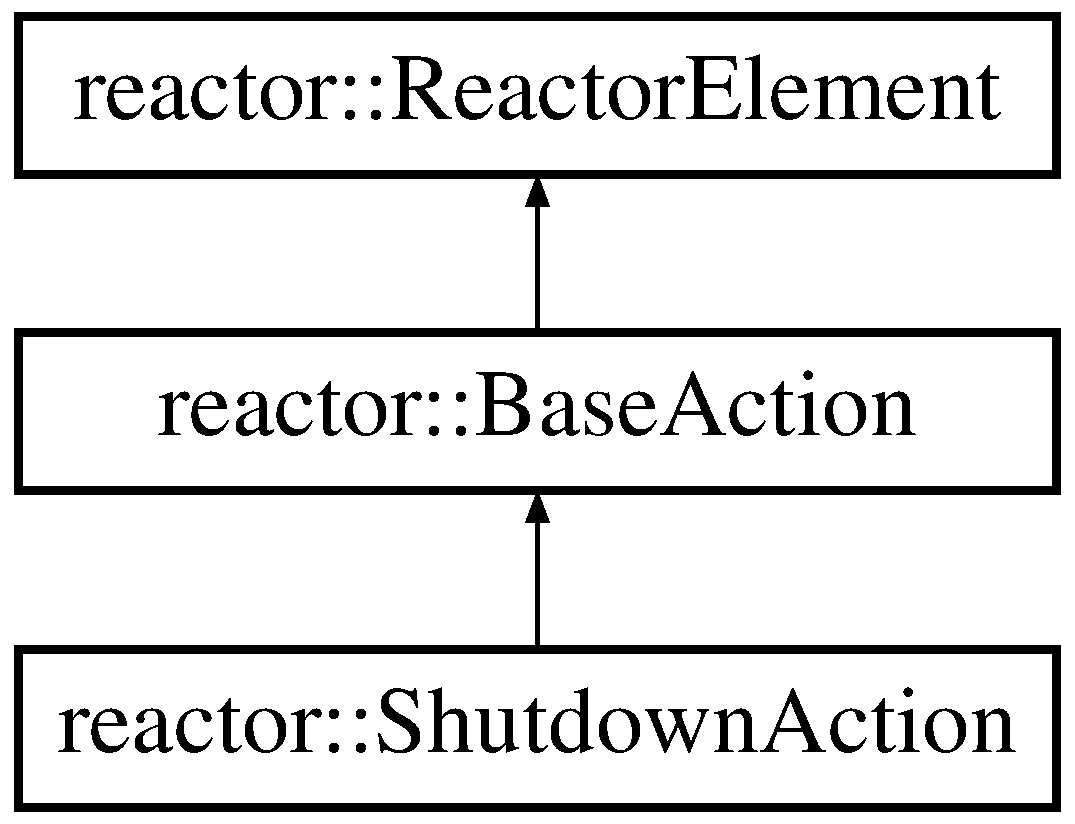
\includegraphics[height=3.000000cm]{classreactor_1_1ShutdownAction}
\end{center}
\end{figure}
\subsection*{Public Member Functions}
\begin{DoxyCompactItemize}
\item 
\hyperlink{classreactor_1_1ShutdownAction_a9b0444bd81eaca6f1b51f484ee0b95b2}{Shutdown\+Action} (const std\+::string \&\hyperlink{classreactor_1_1ReactorElement_a99579f61dbaf5d5d98aebfe26eb8bf77}{name}, \hyperlink{classreactor_1_1Reactor}{Reactor} $\ast$\hyperlink{classreactor_1_1ReactorElement_a25bf298de879a82eefc1ba426be05812}{container})
\item 
void \hyperlink{classreactor_1_1ShutdownAction_acbea47c7b7efb26cd10d6ac8c781901a}{cleanup} () override final
\item 
void \hyperlink{classreactor_1_1ShutdownAction_a21c23857012b384cd06f55e002291824}{startup} () override final
\item 
void \hyperlink{classreactor_1_1ShutdownAction_a8950ffd9b67f4800b75a95af92c4fd2a}{shutdown} () override final
\end{DoxyCompactItemize}
\subsection*{Additional Inherited Members}


\subsection{Constructor \& Destructor Documentation}
\mbox{\Hypertarget{classreactor_1_1ShutdownAction_a9b0444bd81eaca6f1b51f484ee0b95b2}\label{classreactor_1_1ShutdownAction_a9b0444bd81eaca6f1b51f484ee0b95b2}} 
\index{reactor\+::\+Shutdown\+Action@{reactor\+::\+Shutdown\+Action}!Shutdown\+Action@{Shutdown\+Action}}
\index{Shutdown\+Action@{Shutdown\+Action}!reactor\+::\+Shutdown\+Action@{reactor\+::\+Shutdown\+Action}}
\subsubsection{\texorpdfstring{Shutdown\+Action()}{ShutdownAction()}}
{\footnotesize\ttfamily reactor\+::\+Shutdown\+Action\+::\+Shutdown\+Action (\begin{DoxyParamCaption}\item[{const std\+::string \&}]{name,  }\item[{\hyperlink{classreactor_1_1Reactor}{Reactor} $\ast$}]{container }\end{DoxyParamCaption})\hspace{0.3cm}{\ttfamily [inline]}}



\subsection{Member Function Documentation}
\mbox{\Hypertarget{classreactor_1_1ShutdownAction_acbea47c7b7efb26cd10d6ac8c781901a}\label{classreactor_1_1ShutdownAction_acbea47c7b7efb26cd10d6ac8c781901a}} 
\index{reactor\+::\+Shutdown\+Action@{reactor\+::\+Shutdown\+Action}!cleanup@{cleanup}}
\index{cleanup@{cleanup}!reactor\+::\+Shutdown\+Action@{reactor\+::\+Shutdown\+Action}}
\subsubsection{\texorpdfstring{cleanup()}{cleanup()}}
{\footnotesize\ttfamily void reactor\+::\+Shutdown\+Action\+::cleanup (\begin{DoxyParamCaption}{ }\end{DoxyParamCaption})\hspace{0.3cm}{\ttfamily [inline]}, {\ttfamily [final]}, {\ttfamily [override]}, {\ttfamily [virtual]}}



Implements \hyperlink{classreactor_1_1BaseAction_a7e4ad7157e653054c7afa22b78e46923}{reactor\+::\+Base\+Action}.

\mbox{\Hypertarget{classreactor_1_1ShutdownAction_a8950ffd9b67f4800b75a95af92c4fd2a}\label{classreactor_1_1ShutdownAction_a8950ffd9b67f4800b75a95af92c4fd2a}} 
\index{reactor\+::\+Shutdown\+Action@{reactor\+::\+Shutdown\+Action}!shutdown@{shutdown}}
\index{shutdown@{shutdown}!reactor\+::\+Shutdown\+Action@{reactor\+::\+Shutdown\+Action}}
\subsubsection{\texorpdfstring{shutdown()}{shutdown()}}
{\footnotesize\ttfamily void reactor\+::\+Shutdown\+Action\+::shutdown (\begin{DoxyParamCaption}{ }\end{DoxyParamCaption})\hspace{0.3cm}{\ttfamily [final]}, {\ttfamily [override]}, {\ttfamily [virtual]}}



Implements \hyperlink{classreactor_1_1ReactorElement_a8fce084bef582156979ebba56737e907}{reactor\+::\+Reactor\+Element}.

\mbox{\Hypertarget{classreactor_1_1ShutdownAction_a21c23857012b384cd06f55e002291824}\label{classreactor_1_1ShutdownAction_a21c23857012b384cd06f55e002291824}} 
\index{reactor\+::\+Shutdown\+Action@{reactor\+::\+Shutdown\+Action}!startup@{startup}}
\index{startup@{startup}!reactor\+::\+Shutdown\+Action@{reactor\+::\+Shutdown\+Action}}
\subsubsection{\texorpdfstring{startup()}{startup()}}
{\footnotesize\ttfamily void reactor\+::\+Shutdown\+Action\+::startup (\begin{DoxyParamCaption}{ }\end{DoxyParamCaption})\hspace{0.3cm}{\ttfamily [inline]}, {\ttfamily [final]}, {\ttfamily [override]}, {\ttfamily [virtual]}}



Implements \hyperlink{classreactor_1_1ReactorElement_a8cb574cb20ff963903ad905fb0a157e3}{reactor\+::\+Reactor\+Element}.



The documentation for this class was generated from the following files\+:\begin{DoxyCompactItemize}
\item 
/home/runner/work/reactor-\/cpp/reactor-\/cpp/include/reactor-\/cpp/\hyperlink{action_8hh}{action.\+hh}\item 
/home/runner/work/reactor-\/cpp/reactor-\/cpp/lib/\hyperlink{action_8cc}{action.\+cc}\end{DoxyCompactItemize}

\hypertarget{classreactor_1_1StartupAction}{}\section{reactor\+:\+:Startup\+Action Class Reference}
\label{classreactor_1_1StartupAction}\index{reactor\+::\+Startup\+Action@{reactor\+::\+Startup\+Action}}


{\ttfamily \#include $<$action.\+hh$>$}

Inheritance diagram for reactor\+:\+:Startup\+Action\+:\begin{figure}[H]
\begin{center}
\leavevmode
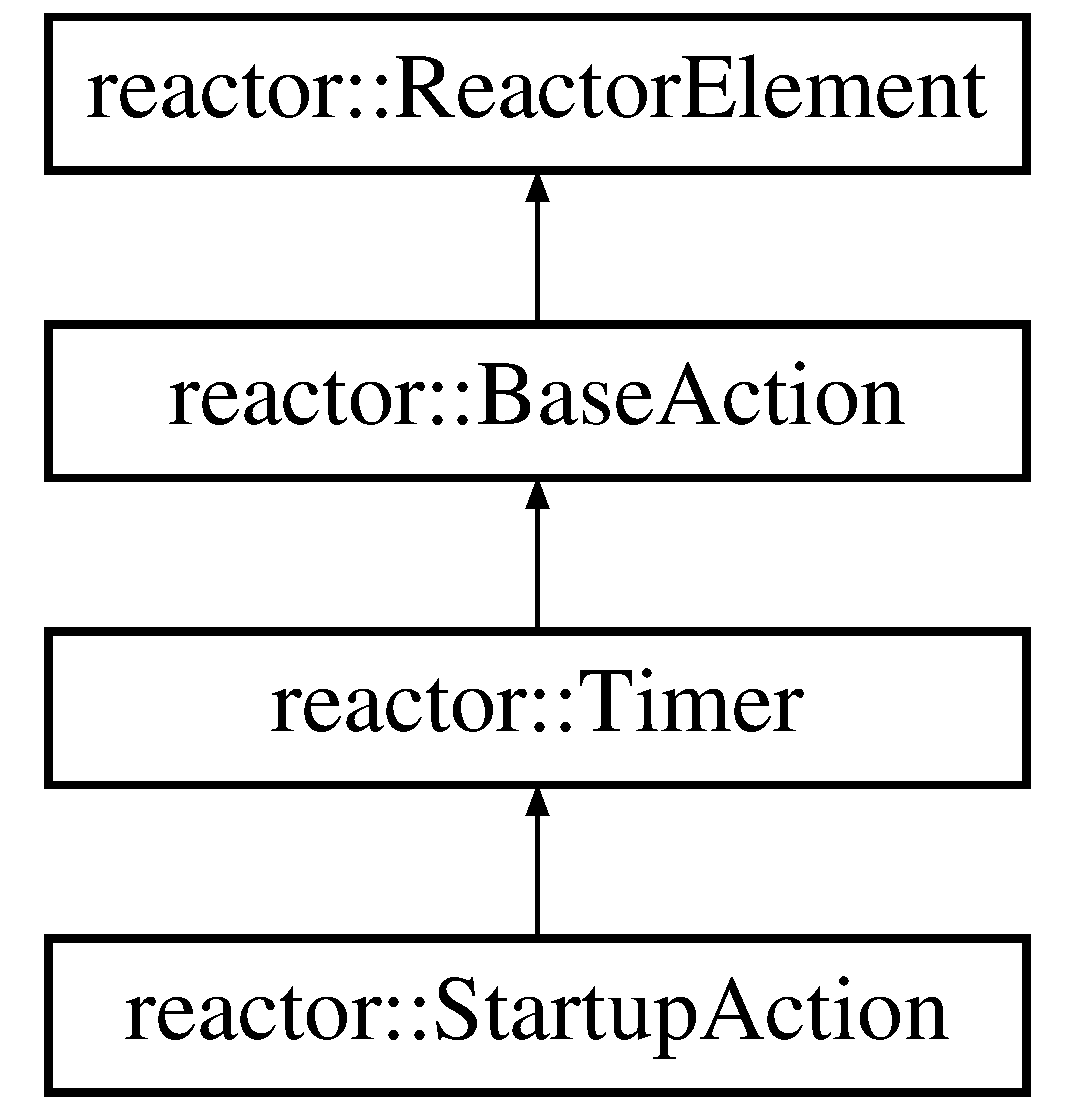
\includegraphics[height=4.000000cm]{classreactor_1_1StartupAction}
\end{center}
\end{figure}
\subsection*{Public Member Functions}
\begin{DoxyCompactItemize}
\item 
\hyperlink{classreactor_1_1StartupAction_a6377de4a00c57020dbb7cd0d9eb82bce}{Startup\+Action} (const std\+::string \&\hyperlink{classreactor_1_1ReactorElement_a99579f61dbaf5d5d98aebfe26eb8bf77}{name}, \hyperlink{classreactor_1_1Reactor}{Reactor} $\ast$\hyperlink{classreactor_1_1ReactorElement_a25bf298de879a82eefc1ba426be05812}{container})
\end{DoxyCompactItemize}
\subsection*{Additional Inherited Members}


\subsection{Constructor \& Destructor Documentation}
\mbox{\Hypertarget{classreactor_1_1StartupAction_a6377de4a00c57020dbb7cd0d9eb82bce}\label{classreactor_1_1StartupAction_a6377de4a00c57020dbb7cd0d9eb82bce}} 
\index{reactor\+::\+Startup\+Action@{reactor\+::\+Startup\+Action}!Startup\+Action@{Startup\+Action}}
\index{Startup\+Action@{Startup\+Action}!reactor\+::\+Startup\+Action@{reactor\+::\+Startup\+Action}}
\subsubsection{\texorpdfstring{Startup\+Action()}{StartupAction()}}
{\footnotesize\ttfamily reactor\+::\+Startup\+Action\+::\+Startup\+Action (\begin{DoxyParamCaption}\item[{const std\+::string \&}]{name,  }\item[{\hyperlink{classreactor_1_1Reactor}{Reactor} $\ast$}]{container }\end{DoxyParamCaption})\hspace{0.3cm}{\ttfamily [inline]}}



The documentation for this class was generated from the following file\+:\begin{DoxyCompactItemize}
\item 
/home/runner/work/reactor-\/cpp/reactor-\/cpp/include/reactor-\/cpp/\hyperlink{action_8hh}{action.\+hh}\end{DoxyCompactItemize}

\hypertarget{classreactor_1_1Tag}{}\section{reactor\+:\+:Tag Class Reference}
\label{classreactor_1_1Tag}\index{reactor\+::\+Tag@{reactor\+::\+Tag}}


{\ttfamily \#include $<$logical\+\_\+time.\+hh$>$}

\subsection*{Public Member Functions}
\begin{DoxyCompactItemize}
\item 
\hyperlink{classreactor_1_1Tag_a25458048eeb77969069faee12894f6d4}{Tag} ()=delete
\item 
\hyperlink{classreactor_1_1Tag}{Tag} \& \hyperlink{classreactor_1_1Tag_ae0776e16fba93c8836ab0d1651ffd309}{operator=} (const \hyperlink{classreactor_1_1Tag}{Tag} \&)=delete
\item 
\hyperlink{classreactor_1_1Tag_aa810576d4b247523df94a623e36acbb3}{Tag} (\hyperlink{classreactor_1_1Tag}{Tag} \&\&)=default
\item 
\hyperlink{classreactor_1_1Tag_a83b08304268878143b98f83b0e6400ba}{Tag} (const \hyperlink{classreactor_1_1Tag}{Tag} \&)=default
\item 
const \hyperlink{namespacereactor_ad950f8d1a46612500286a4af0f167080}{Time\+Point} \& \hyperlink{classreactor_1_1Tag_a25ec5662af4fc8c9b34cf5cc0d70b569}{time\+\_\+point} () const
\item 
const \hyperlink{namespacereactor_aaea1189d617982457b74127ba74a7340}{mstep\+\_\+t} \& \hyperlink{classreactor_1_1Tag_a8cfdeeb03c2e48a684e1bc517505c087}{micro\+\_\+step} () const
\item 
\hyperlink{classreactor_1_1Tag}{Tag} \hyperlink{classreactor_1_1Tag_af4cf8dfbcef78f120e71562084e67168}{delay} (\hyperlink{namespacereactor_aa8375b807a80703545664096c5b5b779}{Duration} offset=Duration\+::zero()) const
\end{DoxyCompactItemize}
\subsection*{Static Public Member Functions}
\begin{DoxyCompactItemize}
\item 
static \hyperlink{classreactor_1_1Tag}{Tag} \hyperlink{classreactor_1_1Tag_ad0577aba35a17c5aac3dec8629977ae1}{from\+\_\+physical\+\_\+time} (\hyperlink{namespacereactor_ad950f8d1a46612500286a4af0f167080}{Time\+Point} \hyperlink{classreactor_1_1Tag_a25ec5662af4fc8c9b34cf5cc0d70b569}{time\+\_\+point})
\item 
static \hyperlink{classreactor_1_1Tag}{Tag} \hyperlink{classreactor_1_1Tag_a99d7fef2a7b8f865e8d69d45ea9cf17f}{from\+\_\+logical\+\_\+time} (const \hyperlink{classreactor_1_1LogicalTime}{Logical\+Time} \&lt)
\end{DoxyCompactItemize}
\subsection*{Private Member Functions}
\begin{DoxyCompactItemize}
\item 
\hyperlink{classreactor_1_1Tag_ae9912e50f1398a241205e8fae7ad9cea}{Tag} (const \hyperlink{namespacereactor_ad950f8d1a46612500286a4af0f167080}{Time\+Point} \&\hyperlink{classreactor_1_1Tag_a25ec5662af4fc8c9b34cf5cc0d70b569}{time\+\_\+point}, const \hyperlink{namespacereactor_aaea1189d617982457b74127ba74a7340}{mstep\+\_\+t} \&\hyperlink{classreactor_1_1Tag_a8cfdeeb03c2e48a684e1bc517505c087}{micro\+\_\+step})
\end{DoxyCompactItemize}
\subsection*{Private Attributes}
\begin{DoxyCompactItemize}
\item 
const \hyperlink{namespacereactor_ad950f8d1a46612500286a4af0f167080}{Time\+Point} \hyperlink{classreactor_1_1Tag_a24a75e25cfaac63128d8f925ee95c4d9}{\+\_\+time\+\_\+point}
\item 
const \hyperlink{namespacereactor_aaea1189d617982457b74127ba74a7340}{mstep\+\_\+t} \hyperlink{classreactor_1_1Tag_a7660e5c962c9916a04abe97fad3226ab}{\+\_\+micro\+\_\+step}
\end{DoxyCompactItemize}


\subsection{Constructor \& Destructor Documentation}
\mbox{\Hypertarget{classreactor_1_1Tag_ae9912e50f1398a241205e8fae7ad9cea}\label{classreactor_1_1Tag_ae9912e50f1398a241205e8fae7ad9cea}} 
\index{reactor\+::\+Tag@{reactor\+::\+Tag}!Tag@{Tag}}
\index{Tag@{Tag}!reactor\+::\+Tag@{reactor\+::\+Tag}}
\subsubsection{\texorpdfstring{Tag()}{Tag()}\hspace{0.1cm}{\footnotesize\ttfamily [1/4]}}
{\footnotesize\ttfamily reactor\+::\+Tag\+::\+Tag (\begin{DoxyParamCaption}\item[{const \hyperlink{namespacereactor_ad950f8d1a46612500286a4af0f167080}{Time\+Point} \&}]{time\+\_\+point,  }\item[{const \hyperlink{namespacereactor_aaea1189d617982457b74127ba74a7340}{mstep\+\_\+t} \&}]{micro\+\_\+step }\end{DoxyParamCaption})\hspace{0.3cm}{\ttfamily [inline]}, {\ttfamily [private]}}

\mbox{\Hypertarget{classreactor_1_1Tag_a25458048eeb77969069faee12894f6d4}\label{classreactor_1_1Tag_a25458048eeb77969069faee12894f6d4}} 
\index{reactor\+::\+Tag@{reactor\+::\+Tag}!Tag@{Tag}}
\index{Tag@{Tag}!reactor\+::\+Tag@{reactor\+::\+Tag}}
\subsubsection{\texorpdfstring{Tag()}{Tag()}\hspace{0.1cm}{\footnotesize\ttfamily [2/4]}}
{\footnotesize\ttfamily reactor\+::\+Tag\+::\+Tag (\begin{DoxyParamCaption}{ }\end{DoxyParamCaption})\hspace{0.3cm}{\ttfamily [delete]}}

\mbox{\Hypertarget{classreactor_1_1Tag_aa810576d4b247523df94a623e36acbb3}\label{classreactor_1_1Tag_aa810576d4b247523df94a623e36acbb3}} 
\index{reactor\+::\+Tag@{reactor\+::\+Tag}!Tag@{Tag}}
\index{Tag@{Tag}!reactor\+::\+Tag@{reactor\+::\+Tag}}
\subsubsection{\texorpdfstring{Tag()}{Tag()}\hspace{0.1cm}{\footnotesize\ttfamily [3/4]}}
{\footnotesize\ttfamily reactor\+::\+Tag\+::\+Tag (\begin{DoxyParamCaption}\item[{\hyperlink{classreactor_1_1Tag}{Tag} \&\&}]{ }\end{DoxyParamCaption})\hspace{0.3cm}{\ttfamily [default]}}

\mbox{\Hypertarget{classreactor_1_1Tag_a83b08304268878143b98f83b0e6400ba}\label{classreactor_1_1Tag_a83b08304268878143b98f83b0e6400ba}} 
\index{reactor\+::\+Tag@{reactor\+::\+Tag}!Tag@{Tag}}
\index{Tag@{Tag}!reactor\+::\+Tag@{reactor\+::\+Tag}}
\subsubsection{\texorpdfstring{Tag()}{Tag()}\hspace{0.1cm}{\footnotesize\ttfamily [4/4]}}
{\footnotesize\ttfamily reactor\+::\+Tag\+::\+Tag (\begin{DoxyParamCaption}\item[{const \hyperlink{classreactor_1_1Tag}{Tag} \&}]{ }\end{DoxyParamCaption})\hspace{0.3cm}{\ttfamily [default]}}



\subsection{Member Function Documentation}
\mbox{\Hypertarget{classreactor_1_1Tag_af4cf8dfbcef78f120e71562084e67168}\label{classreactor_1_1Tag_af4cf8dfbcef78f120e71562084e67168}} 
\index{reactor\+::\+Tag@{reactor\+::\+Tag}!delay@{delay}}
\index{delay@{delay}!reactor\+::\+Tag@{reactor\+::\+Tag}}
\subsubsection{\texorpdfstring{delay()}{delay()}}
{\footnotesize\ttfamily \hyperlink{classreactor_1_1Tag}{Tag} reactor\+::\+Tag\+::delay (\begin{DoxyParamCaption}\item[{\hyperlink{namespacereactor_aa8375b807a80703545664096c5b5b779}{Duration}}]{offset = {\ttfamily Duration\+:\+:zero()} }\end{DoxyParamCaption}) const}

\mbox{\Hypertarget{classreactor_1_1Tag_a99d7fef2a7b8f865e8d69d45ea9cf17f}\label{classreactor_1_1Tag_a99d7fef2a7b8f865e8d69d45ea9cf17f}} 
\index{reactor\+::\+Tag@{reactor\+::\+Tag}!from\+\_\+logical\+\_\+time@{from\+\_\+logical\+\_\+time}}
\index{from\+\_\+logical\+\_\+time@{from\+\_\+logical\+\_\+time}!reactor\+::\+Tag@{reactor\+::\+Tag}}
\subsubsection{\texorpdfstring{from\+\_\+logical\+\_\+time()}{from\_logical\_time()}}
{\footnotesize\ttfamily \hyperlink{classreactor_1_1Tag}{Tag} reactor\+::\+Tag\+::from\+\_\+logical\+\_\+time (\begin{DoxyParamCaption}\item[{const \hyperlink{classreactor_1_1LogicalTime}{Logical\+Time} \&}]{lt }\end{DoxyParamCaption})\hspace{0.3cm}{\ttfamily [static]}}

\mbox{\Hypertarget{classreactor_1_1Tag_ad0577aba35a17c5aac3dec8629977ae1}\label{classreactor_1_1Tag_ad0577aba35a17c5aac3dec8629977ae1}} 
\index{reactor\+::\+Tag@{reactor\+::\+Tag}!from\+\_\+physical\+\_\+time@{from\+\_\+physical\+\_\+time}}
\index{from\+\_\+physical\+\_\+time@{from\+\_\+physical\+\_\+time}!reactor\+::\+Tag@{reactor\+::\+Tag}}
\subsubsection{\texorpdfstring{from\+\_\+physical\+\_\+time()}{from\_physical\_time()}}
{\footnotesize\ttfamily \hyperlink{classreactor_1_1Tag}{Tag} reactor\+::\+Tag\+::from\+\_\+physical\+\_\+time (\begin{DoxyParamCaption}\item[{\hyperlink{namespacereactor_ad950f8d1a46612500286a4af0f167080}{Time\+Point}}]{time\+\_\+point }\end{DoxyParamCaption})\hspace{0.3cm}{\ttfamily [static]}}

\mbox{\Hypertarget{classreactor_1_1Tag_a8cfdeeb03c2e48a684e1bc517505c087}\label{classreactor_1_1Tag_a8cfdeeb03c2e48a684e1bc517505c087}} 
\index{reactor\+::\+Tag@{reactor\+::\+Tag}!micro\+\_\+step@{micro\+\_\+step}}
\index{micro\+\_\+step@{micro\+\_\+step}!reactor\+::\+Tag@{reactor\+::\+Tag}}
\subsubsection{\texorpdfstring{micro\+\_\+step()}{micro\_step()}}
{\footnotesize\ttfamily const \hyperlink{namespacereactor_aaea1189d617982457b74127ba74a7340}{mstep\+\_\+t}\& reactor\+::\+Tag\+::micro\+\_\+step (\begin{DoxyParamCaption}{ }\end{DoxyParamCaption}) const\hspace{0.3cm}{\ttfamily [inline]}}

\mbox{\Hypertarget{classreactor_1_1Tag_ae0776e16fba93c8836ab0d1651ffd309}\label{classreactor_1_1Tag_ae0776e16fba93c8836ab0d1651ffd309}} 
\index{reactor\+::\+Tag@{reactor\+::\+Tag}!operator=@{operator=}}
\index{operator=@{operator=}!reactor\+::\+Tag@{reactor\+::\+Tag}}
\subsubsection{\texorpdfstring{operator=()}{operator=()}}
{\footnotesize\ttfamily \hyperlink{classreactor_1_1Tag}{Tag}\& reactor\+::\+Tag\+::operator= (\begin{DoxyParamCaption}\item[{const \hyperlink{classreactor_1_1Tag}{Tag} \&}]{ }\end{DoxyParamCaption})\hspace{0.3cm}{\ttfamily [delete]}}

\mbox{\Hypertarget{classreactor_1_1Tag_a25ec5662af4fc8c9b34cf5cc0d70b569}\label{classreactor_1_1Tag_a25ec5662af4fc8c9b34cf5cc0d70b569}} 
\index{reactor\+::\+Tag@{reactor\+::\+Tag}!time\+\_\+point@{time\+\_\+point}}
\index{time\+\_\+point@{time\+\_\+point}!reactor\+::\+Tag@{reactor\+::\+Tag}}
\subsubsection{\texorpdfstring{time\+\_\+point()}{time\_point()}}
{\footnotesize\ttfamily const \hyperlink{namespacereactor_ad950f8d1a46612500286a4af0f167080}{Time\+Point}\& reactor\+::\+Tag\+::time\+\_\+point (\begin{DoxyParamCaption}{ }\end{DoxyParamCaption}) const\hspace{0.3cm}{\ttfamily [inline]}}



\subsection{Member Data Documentation}
\mbox{\Hypertarget{classreactor_1_1Tag_a7660e5c962c9916a04abe97fad3226ab}\label{classreactor_1_1Tag_a7660e5c962c9916a04abe97fad3226ab}} 
\index{reactor\+::\+Tag@{reactor\+::\+Tag}!\+\_\+micro\+\_\+step@{\+\_\+micro\+\_\+step}}
\index{\+\_\+micro\+\_\+step@{\+\_\+micro\+\_\+step}!reactor\+::\+Tag@{reactor\+::\+Tag}}
\subsubsection{\texorpdfstring{\+\_\+micro\+\_\+step}{\_micro\_step}}
{\footnotesize\ttfamily const \hyperlink{namespacereactor_aaea1189d617982457b74127ba74a7340}{mstep\+\_\+t} reactor\+::\+Tag\+::\+\_\+micro\+\_\+step\hspace{0.3cm}{\ttfamily [private]}}

\mbox{\Hypertarget{classreactor_1_1Tag_a24a75e25cfaac63128d8f925ee95c4d9}\label{classreactor_1_1Tag_a24a75e25cfaac63128d8f925ee95c4d9}} 
\index{reactor\+::\+Tag@{reactor\+::\+Tag}!\+\_\+time\+\_\+point@{\+\_\+time\+\_\+point}}
\index{\+\_\+time\+\_\+point@{\+\_\+time\+\_\+point}!reactor\+::\+Tag@{reactor\+::\+Tag}}
\subsubsection{\texorpdfstring{\+\_\+time\+\_\+point}{\_time\_point}}
{\footnotesize\ttfamily const \hyperlink{namespacereactor_ad950f8d1a46612500286a4af0f167080}{Time\+Point} reactor\+::\+Tag\+::\+\_\+time\+\_\+point\hspace{0.3cm}{\ttfamily [private]}}



The documentation for this class was generated from the following files\+:\begin{DoxyCompactItemize}
\item 
/home/runner/work/reactor-\/cpp/reactor-\/cpp/include/reactor-\/cpp/\hyperlink{logical__time_8hh}{logical\+\_\+time.\+hh}\item 
/home/runner/work/reactor-\/cpp/reactor-\/cpp/lib/\hyperlink{logical__time_8cc}{logical\+\_\+time.\+cc}\end{DoxyCompactItemize}

\hypertarget{classreactor_1_1Timer}{}\section{reactor\+:\+:Timer Class Reference}
\label{classreactor_1_1Timer}\index{reactor\+::\+Timer@{reactor\+::\+Timer}}


{\ttfamily \#include $<$action.\+hh$>$}

Inheritance diagram for reactor\+:\+:Timer\+:\begin{figure}[H]
\begin{center}
\leavevmode
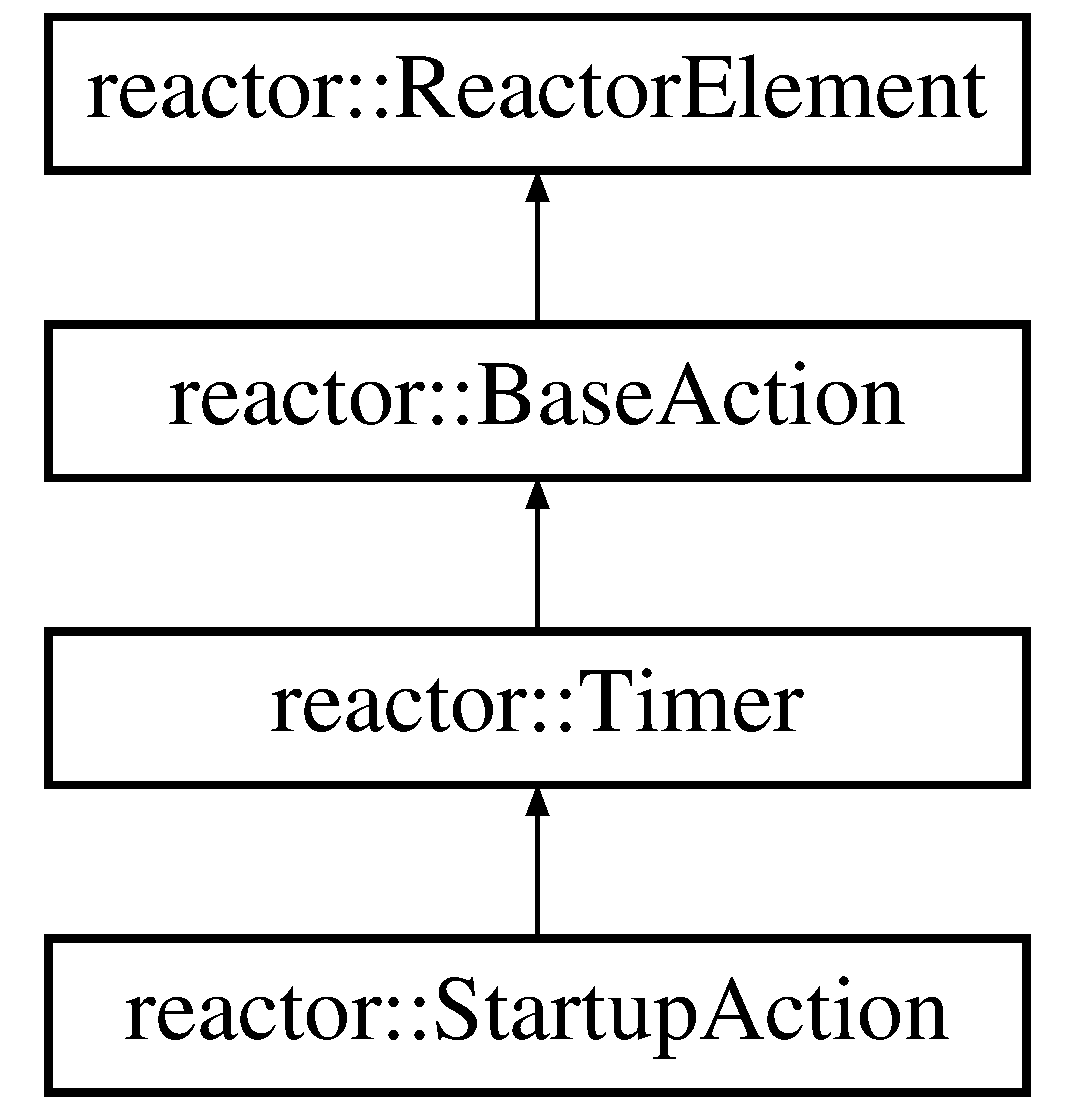
\includegraphics[height=4.000000cm]{classreactor_1_1Timer}
\end{center}
\end{figure}
\subsection*{Public Member Functions}
\begin{DoxyCompactItemize}
\item 
\hyperlink{classreactor_1_1Timer_a54e32e02f2374d4cb4097618cb6181a2}{Timer} (const std\+::string \&\hyperlink{classreactor_1_1ReactorElement_a99579f61dbaf5d5d98aebfe26eb8bf77}{name}, \hyperlink{classreactor_1_1Reactor}{Reactor} $\ast$\hyperlink{classreactor_1_1ReactorElement_a25bf298de879a82eefc1ba426be05812}{container}, \hyperlink{namespacereactor_aa8375b807a80703545664096c5b5b779}{Duration} \hyperlink{classreactor_1_1Timer_a618e80997d7d4881df1b9e9190dae82d}{period}=Duration\+::zero(), \hyperlink{namespacereactor_aa8375b807a80703545664096c5b5b779}{Duration} \hyperlink{classreactor_1_1Timer_ad88516bbbba6a4380bae74af76611640}{offset}=Duration\+::zero())
\item 
void \hyperlink{classreactor_1_1Timer_af820c0879317afb9b98ddc890ac96271}{startup} () override final
\item 
void \hyperlink{classreactor_1_1Timer_a35f218aab3bf72b87cff4aa984dee991}{shutdown} () override final
\item 
const \hyperlink{namespacereactor_aa8375b807a80703545664096c5b5b779}{Duration} \& \hyperlink{classreactor_1_1Timer_ad88516bbbba6a4380bae74af76611640}{offset} () const
\item 
const \hyperlink{namespacereactor_aa8375b807a80703545664096c5b5b779}{Duration} \& \hyperlink{classreactor_1_1Timer_a618e80997d7d4881df1b9e9190dae82d}{period} () const
\end{DoxyCompactItemize}
\subsection*{Private Member Functions}
\begin{DoxyCompactItemize}
\item 
void \hyperlink{classreactor_1_1Timer_a24cde6fc75c1098f9941ce80a5b7f814}{reschedule} ()
\item 
void \hyperlink{classreactor_1_1Timer_ab01356b0c99de6a3bd9f46bfd0ce1c7b}{cleanup} () override final
\end{DoxyCompactItemize}
\subsection*{Private Attributes}
\begin{DoxyCompactItemize}
\item 
const \hyperlink{namespacereactor_aa8375b807a80703545664096c5b5b779}{Duration} \hyperlink{classreactor_1_1Timer_ae3f332ade1a8caf90db054024dcf931b}{\+\_\+offset}
\item 
const \hyperlink{namespacereactor_aa8375b807a80703545664096c5b5b779}{Duration} \hyperlink{classreactor_1_1Timer_a3524de2cc02985e98ee7115300adc452}{\+\_\+period}
\end{DoxyCompactItemize}
\subsection*{Additional Inherited Members}


\subsection{Constructor \& Destructor Documentation}
\mbox{\Hypertarget{classreactor_1_1Timer_a54e32e02f2374d4cb4097618cb6181a2}\label{classreactor_1_1Timer_a54e32e02f2374d4cb4097618cb6181a2}} 
\index{reactor\+::\+Timer@{reactor\+::\+Timer}!Timer@{Timer}}
\index{Timer@{Timer}!reactor\+::\+Timer@{reactor\+::\+Timer}}
\subsubsection{\texorpdfstring{Timer()}{Timer()}}
{\footnotesize\ttfamily reactor\+::\+Timer\+::\+Timer (\begin{DoxyParamCaption}\item[{const std\+::string \&}]{name,  }\item[{\hyperlink{classreactor_1_1Reactor}{Reactor} $\ast$}]{container,  }\item[{\hyperlink{namespacereactor_aa8375b807a80703545664096c5b5b779}{Duration}}]{period = {\ttfamily Duration\+:\+:zero()},  }\item[{\hyperlink{namespacereactor_aa8375b807a80703545664096c5b5b779}{Duration}}]{offset = {\ttfamily Duration\+:\+:zero()} }\end{DoxyParamCaption})\hspace{0.3cm}{\ttfamily [inline]}}



\subsection{Member Function Documentation}
\mbox{\Hypertarget{classreactor_1_1Timer_ab01356b0c99de6a3bd9f46bfd0ce1c7b}\label{classreactor_1_1Timer_ab01356b0c99de6a3bd9f46bfd0ce1c7b}} 
\index{reactor\+::\+Timer@{reactor\+::\+Timer}!cleanup@{cleanup}}
\index{cleanup@{cleanup}!reactor\+::\+Timer@{reactor\+::\+Timer}}
\subsubsection{\texorpdfstring{cleanup()}{cleanup()}}
{\footnotesize\ttfamily void reactor\+::\+Timer\+::cleanup (\begin{DoxyParamCaption}{ }\end{DoxyParamCaption})\hspace{0.3cm}{\ttfamily [final]}, {\ttfamily [override]}, {\ttfamily [private]}, {\ttfamily [virtual]}}



Implements \hyperlink{classreactor_1_1BaseAction_a7e4ad7157e653054c7afa22b78e46923}{reactor\+::\+Base\+Action}.

\mbox{\Hypertarget{classreactor_1_1Timer_ad88516bbbba6a4380bae74af76611640}\label{classreactor_1_1Timer_ad88516bbbba6a4380bae74af76611640}} 
\index{reactor\+::\+Timer@{reactor\+::\+Timer}!offset@{offset}}
\index{offset@{offset}!reactor\+::\+Timer@{reactor\+::\+Timer}}
\subsubsection{\texorpdfstring{offset()}{offset()}}
{\footnotesize\ttfamily const \hyperlink{namespacereactor_aa8375b807a80703545664096c5b5b779}{Duration}\& reactor\+::\+Timer\+::offset (\begin{DoxyParamCaption}{ }\end{DoxyParamCaption}) const\hspace{0.3cm}{\ttfamily [inline]}}

\mbox{\Hypertarget{classreactor_1_1Timer_a618e80997d7d4881df1b9e9190dae82d}\label{classreactor_1_1Timer_a618e80997d7d4881df1b9e9190dae82d}} 
\index{reactor\+::\+Timer@{reactor\+::\+Timer}!period@{period}}
\index{period@{period}!reactor\+::\+Timer@{reactor\+::\+Timer}}
\subsubsection{\texorpdfstring{period()}{period()}}
{\footnotesize\ttfamily const \hyperlink{namespacereactor_aa8375b807a80703545664096c5b5b779}{Duration}\& reactor\+::\+Timer\+::period (\begin{DoxyParamCaption}{ }\end{DoxyParamCaption}) const\hspace{0.3cm}{\ttfamily [inline]}}

\mbox{\Hypertarget{classreactor_1_1Timer_a24cde6fc75c1098f9941ce80a5b7f814}\label{classreactor_1_1Timer_a24cde6fc75c1098f9941ce80a5b7f814}} 
\index{reactor\+::\+Timer@{reactor\+::\+Timer}!reschedule@{reschedule}}
\index{reschedule@{reschedule}!reactor\+::\+Timer@{reactor\+::\+Timer}}
\subsubsection{\texorpdfstring{reschedule()}{reschedule()}}
{\footnotesize\ttfamily void reactor\+::\+Timer\+::reschedule (\begin{DoxyParamCaption}{ }\end{DoxyParamCaption})\hspace{0.3cm}{\ttfamily [private]}}

\mbox{\Hypertarget{classreactor_1_1Timer_a35f218aab3bf72b87cff4aa984dee991}\label{classreactor_1_1Timer_a35f218aab3bf72b87cff4aa984dee991}} 
\index{reactor\+::\+Timer@{reactor\+::\+Timer}!shutdown@{shutdown}}
\index{shutdown@{shutdown}!reactor\+::\+Timer@{reactor\+::\+Timer}}
\subsubsection{\texorpdfstring{shutdown()}{shutdown()}}
{\footnotesize\ttfamily void reactor\+::\+Timer\+::shutdown (\begin{DoxyParamCaption}{ }\end{DoxyParamCaption})\hspace{0.3cm}{\ttfamily [inline]}, {\ttfamily [final]}, {\ttfamily [override]}, {\ttfamily [virtual]}}



Implements \hyperlink{classreactor_1_1ReactorElement_a8fce084bef582156979ebba56737e907}{reactor\+::\+Reactor\+Element}.

\mbox{\Hypertarget{classreactor_1_1Timer_af820c0879317afb9b98ddc890ac96271}\label{classreactor_1_1Timer_af820c0879317afb9b98ddc890ac96271}} 
\index{reactor\+::\+Timer@{reactor\+::\+Timer}!startup@{startup}}
\index{startup@{startup}!reactor\+::\+Timer@{reactor\+::\+Timer}}
\subsubsection{\texorpdfstring{startup()}{startup()}}
{\footnotesize\ttfamily void reactor\+::\+Timer\+::startup (\begin{DoxyParamCaption}{ }\end{DoxyParamCaption})\hspace{0.3cm}{\ttfamily [final]}, {\ttfamily [override]}, {\ttfamily [virtual]}}



Implements \hyperlink{classreactor_1_1ReactorElement_a8cb574cb20ff963903ad905fb0a157e3}{reactor\+::\+Reactor\+Element}.



\subsection{Member Data Documentation}
\mbox{\Hypertarget{classreactor_1_1Timer_ae3f332ade1a8caf90db054024dcf931b}\label{classreactor_1_1Timer_ae3f332ade1a8caf90db054024dcf931b}} 
\index{reactor\+::\+Timer@{reactor\+::\+Timer}!\+\_\+offset@{\+\_\+offset}}
\index{\+\_\+offset@{\+\_\+offset}!reactor\+::\+Timer@{reactor\+::\+Timer}}
\subsubsection{\texorpdfstring{\+\_\+offset}{\_offset}}
{\footnotesize\ttfamily const \hyperlink{namespacereactor_aa8375b807a80703545664096c5b5b779}{Duration} reactor\+::\+Timer\+::\+\_\+offset\hspace{0.3cm}{\ttfamily [private]}}

\mbox{\Hypertarget{classreactor_1_1Timer_a3524de2cc02985e98ee7115300adc452}\label{classreactor_1_1Timer_a3524de2cc02985e98ee7115300adc452}} 
\index{reactor\+::\+Timer@{reactor\+::\+Timer}!\+\_\+period@{\+\_\+period}}
\index{\+\_\+period@{\+\_\+period}!reactor\+::\+Timer@{reactor\+::\+Timer}}
\subsubsection{\texorpdfstring{\+\_\+period}{\_period}}
{\footnotesize\ttfamily const \hyperlink{namespacereactor_aa8375b807a80703545664096c5b5b779}{Duration} reactor\+::\+Timer\+::\+\_\+period\hspace{0.3cm}{\ttfamily [private]}}



The documentation for this class was generated from the following files\+:\begin{DoxyCompactItemize}
\item 
/home/runner/work/reactor-\/cpp/reactor-\/cpp/include/reactor-\/cpp/\hyperlink{action_8hh}{action.\+hh}\item 
/home/runner/work/reactor-\/cpp/reactor-\/cpp/lib/\hyperlink{action_8cc}{action.\+cc}\end{DoxyCompactItemize}

\hypertarget{classreactor_1_1ValidationError}{}\section{reactor\+:\+:Validation\+Error Class Reference}
\label{classreactor_1_1ValidationError}\index{reactor\+::\+Validation\+Error@{reactor\+::\+Validation\+Error}}


{\ttfamily \#include $<$assert.\+hh$>$}

Inheritance diagram for reactor\+:\+:Validation\+Error\+:\begin{figure}[H]
\begin{center}
\leavevmode
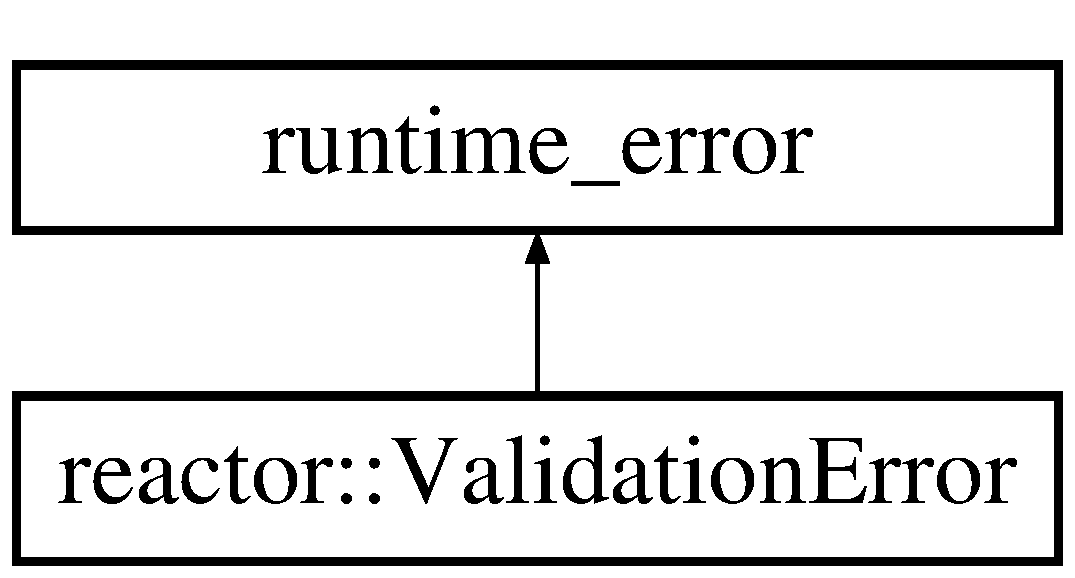
\includegraphics[height=2.000000cm]{classreactor_1_1ValidationError}
\end{center}
\end{figure}
\subsection*{Public Member Functions}
\begin{DoxyCompactItemize}
\item 
\hyperlink{classreactor_1_1ValidationError_a6693659e3b5f0846757304ac38a17deb}{Validation\+Error} (const std\+::string \&msg)
\end{DoxyCompactItemize}
\subsection*{Static Private Member Functions}
\begin{DoxyCompactItemize}
\item 
static std\+::string \hyperlink{classreactor_1_1ValidationError_a5651bea57b5c6ba5e7571172baec633c}{build\+\_\+message} (const std\+::string \&msg)
\end{DoxyCompactItemize}


\subsection{Constructor \& Destructor Documentation}
\mbox{\Hypertarget{classreactor_1_1ValidationError_a6693659e3b5f0846757304ac38a17deb}\label{classreactor_1_1ValidationError_a6693659e3b5f0846757304ac38a17deb}} 
\index{reactor\+::\+Validation\+Error@{reactor\+::\+Validation\+Error}!Validation\+Error@{Validation\+Error}}
\index{Validation\+Error@{Validation\+Error}!reactor\+::\+Validation\+Error@{reactor\+::\+Validation\+Error}}
\subsubsection{\texorpdfstring{Validation\+Error()}{ValidationError()}}
{\footnotesize\ttfamily reactor\+::\+Validation\+Error\+::\+Validation\+Error (\begin{DoxyParamCaption}\item[{const std\+::string \&}]{msg }\end{DoxyParamCaption})\hspace{0.3cm}{\ttfamily [inline]}}



\subsection{Member Function Documentation}
\mbox{\Hypertarget{classreactor_1_1ValidationError_a5651bea57b5c6ba5e7571172baec633c}\label{classreactor_1_1ValidationError_a5651bea57b5c6ba5e7571172baec633c}} 
\index{reactor\+::\+Validation\+Error@{reactor\+::\+Validation\+Error}!build\+\_\+message@{build\+\_\+message}}
\index{build\+\_\+message@{build\+\_\+message}!reactor\+::\+Validation\+Error@{reactor\+::\+Validation\+Error}}
\subsubsection{\texorpdfstring{build\+\_\+message()}{build\_message()}}
{\footnotesize\ttfamily std\+::string reactor\+::\+Validation\+Error\+::build\+\_\+message (\begin{DoxyParamCaption}\item[{const std\+::string \&}]{msg }\end{DoxyParamCaption})\hspace{0.3cm}{\ttfamily [static]}, {\ttfamily [private]}}



The documentation for this class was generated from the following files\+:\begin{DoxyCompactItemize}
\item 
/home/runner/work/reactor-\/cpp/reactor-\/cpp/include/reactor-\/cpp/\hyperlink{assert_8hh}{assert.\+hh}\item 
/home/runner/work/reactor-\/cpp/reactor-\/cpp/lib/\hyperlink{assert_8cc}{assert.\+cc}\end{DoxyCompactItemize}

\hypertarget{structreactor_1_1log_1_1Warn}{}\section{reactor\+:\+:log\+:\+:Warn Struct Reference}
\label{structreactor_1_1log_1_1Warn}\index{reactor\+::log\+::\+Warn@{reactor\+::log\+::\+Warn}}


{\ttfamily \#include $<$logging.\+hh$>$}

Inheritance diagram for reactor\+:\+:log\+:\+:Warn\+:\begin{figure}[H]
\begin{center}
\leavevmode
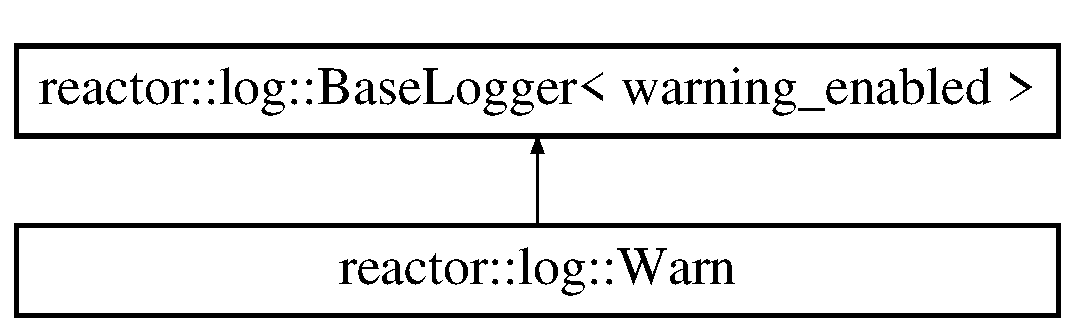
\includegraphics[height=2.000000cm]{structreactor_1_1log_1_1Warn}
\end{center}
\end{figure}
\subsection*{Public Member Functions}
\begin{DoxyCompactItemize}
\item 
\hyperlink{structreactor_1_1log_1_1Warn_ae5618a1eaf8cd1791073c364410152a8}{Warn} ()
\end{DoxyCompactItemize}


\subsection{Constructor \& Destructor Documentation}
\mbox{\Hypertarget{structreactor_1_1log_1_1Warn_ae5618a1eaf8cd1791073c364410152a8}\label{structreactor_1_1log_1_1Warn_ae5618a1eaf8cd1791073c364410152a8}} 
\index{reactor\+::log\+::\+Warn@{reactor\+::log\+::\+Warn}!Warn@{Warn}}
\index{Warn@{Warn}!reactor\+::log\+::\+Warn@{reactor\+::log\+::\+Warn}}
\subsubsection{\texorpdfstring{Warn()}{Warn()}}
{\footnotesize\ttfamily reactor\+::log\+::\+Warn\+::\+Warn (\begin{DoxyParamCaption}{ }\end{DoxyParamCaption})\hspace{0.3cm}{\ttfamily [inline]}}



The documentation for this struct was generated from the following file\+:\begin{DoxyCompactItemize}
\item 
/home/runner/work/reactor-\/cpp/reactor-\/cpp/include/reactor-\/cpp/\hyperlink{logging_8hh}{logging.\+hh}\end{DoxyCompactItemize}

\chapter{File Documentation}
\hypertarget{action_8hh}{}\section{/home/runner/work/reactor-\/cpp/reactor-\/cpp/include/reactor-\/cpp/action.hh File Reference}
\label{action_8hh}\index{/home/runner/work/reactor-\/cpp/reactor-\/cpp/include/reactor-\/cpp/action.\+hh@{/home/runner/work/reactor-\/cpp/reactor-\/cpp/include/reactor-\/cpp/action.\+hh}}
{\ttfamily \#include \char`\"{}logical\+\_\+time.\+hh\char`\"{}}\newline
{\ttfamily \#include \char`\"{}reactor.\+hh\char`\"{}}\newline
{\ttfamily \#include \char`\"{}value\+\_\+ptr.\+hh\char`\"{}}\newline
{\ttfamily \#include \char`\"{}impl/action\+\_\+impl.\+hh\char`\"{}}\newline
\subsection*{Classes}
\begin{DoxyCompactItemize}
\item 
class \hyperlink{classreactor_1_1BaseAction}{reactor\+::\+Base\+Action}
\item 
class \hyperlink{classreactor_1_1Action}{reactor\+::\+Action$<$ T $>$}
\item 
class \hyperlink{classreactor_1_1Action_3_01void_01_4}{reactor\+::\+Action$<$ void $>$}
\item 
class \hyperlink{classreactor_1_1PhysicalAction}{reactor\+::\+Physical\+Action$<$ T $>$}
\item 
class \hyperlink{classreactor_1_1LogicalAction}{reactor\+::\+Logical\+Action$<$ T $>$}
\item 
class \hyperlink{classreactor_1_1Timer}{reactor\+::\+Timer}
\item 
class \hyperlink{classreactor_1_1StartupAction}{reactor\+::\+Startup\+Action}
\item 
class \hyperlink{classreactor_1_1ShutdownAction}{reactor\+::\+Shutdown\+Action}
\end{DoxyCompactItemize}
\subsection*{Namespaces}
\begin{DoxyCompactItemize}
\item 
 \hyperlink{namespacereactor}{reactor}
\end{DoxyCompactItemize}

\hypertarget{assert_8hh}{}\section{/home/runner/work/reactor-\/cpp/reactor-\/cpp/include/reactor-\/cpp/assert.hh File Reference}
\label{assert_8hh}\index{/home/runner/work/reactor-\/cpp/reactor-\/cpp/include/reactor-\/cpp/assert.\+hh@{/home/runner/work/reactor-\/cpp/reactor-\/cpp/include/reactor-\/cpp/assert.\+hh}}
{\ttfamily \#include $<$cassert$>$}\newline
{\ttfamily \#include $<$sstream$>$}\newline
{\ttfamily \#include $<$stdexcept$>$}\newline
{\ttfamily \#include $<$string$>$}\newline
\subsection*{Classes}
\begin{DoxyCompactItemize}
\item 
class \hyperlink{classreactor_1_1ValidationError}{reactor\+::\+Validation\+Error}
\end{DoxyCompactItemize}
\subsection*{Namespaces}
\begin{DoxyCompactItemize}
\item 
 \hyperlink{namespacereactor}{reactor}
\end{DoxyCompactItemize}
\subsection*{Macros}
\begin{DoxyCompactItemize}
\item 
\#define \hyperlink{assert_8hh_aca68c0d4ac8df0838e209fb5300f7be3}{A\+S\+S\+E\+RT}(x)~assert(x)
\item 
\#define \hyperlink{assert_8hh_aa8944c5f0d4c2f0c3643c36ab4967a17}{V\+A\+L\+I\+D\+A\+TE}(con,  msg)
\end{DoxyCompactItemize}
\subsection*{Functions}
\begin{DoxyCompactItemize}
\item 
void \hyperlink{namespacereactor_afb17997129c7498eff1148813c8970d0}{reactor\+::validate} (bool condition, const std\+::string \&message)
\end{DoxyCompactItemize}


\subsection{Macro Definition Documentation}
\mbox{\Hypertarget{assert_8hh_aca68c0d4ac8df0838e209fb5300f7be3}\label{assert_8hh_aca68c0d4ac8df0838e209fb5300f7be3}} 
\index{assert.\+hh@{assert.\+hh}!A\+S\+S\+E\+RT@{A\+S\+S\+E\+RT}}
\index{A\+S\+S\+E\+RT@{A\+S\+S\+E\+RT}!assert.\+hh@{assert.\+hh}}
\subsubsection{\texorpdfstring{A\+S\+S\+E\+RT}{ASSERT}}
{\footnotesize\ttfamily \#define A\+S\+S\+E\+RT(\begin{DoxyParamCaption}\item[{}]{x }\end{DoxyParamCaption})~assert(x)}

\mbox{\Hypertarget{assert_8hh_aa8944c5f0d4c2f0c3643c36ab4967a17}\label{assert_8hh_aa8944c5f0d4c2f0c3643c36ab4967a17}} 
\index{assert.\+hh@{assert.\+hh}!V\+A\+L\+I\+D\+A\+TE@{V\+A\+L\+I\+D\+A\+TE}}
\index{V\+A\+L\+I\+D\+A\+TE@{V\+A\+L\+I\+D\+A\+TE}!assert.\+hh@{assert.\+hh}}
\subsubsection{\texorpdfstring{V\+A\+L\+I\+D\+A\+TE}{VALIDATE}}
{\footnotesize\ttfamily \#define V\+A\+L\+I\+D\+A\+TE(\begin{DoxyParamCaption}\item[{}]{con,  }\item[{}]{msg }\end{DoxyParamCaption})}

{\bfseries Value\+:}
\begin{DoxyCode}
\textcolor{keywordflow}{do} \{               \(\backslash\)
    (void)\textcolor{keyword}{sizeof}(con); \(\backslash\)
  \} \textcolor{keywordflow}{while} (0)
\end{DoxyCode}

\hypertarget{environment_8hh}{}\section{/home/runner/work/reactor-\/cpp/reactor-\/cpp/include/reactor-\/cpp/environment.hh File Reference}
\label{environment_8hh}\index{/home/runner/work/reactor-\/cpp/reactor-\/cpp/include/reactor-\/cpp/environment.\+hh@{/home/runner/work/reactor-\/cpp/reactor-\/cpp/include/reactor-\/cpp/environment.\+hh}}
{\ttfamily \#include $<$set$>$}\newline
{\ttfamily \#include $<$string$>$}\newline
{\ttfamily \#include $<$vector$>$}\newline
{\ttfamily \#include \char`\"{}reactor.\+hh\char`\"{}}\newline
{\ttfamily \#include \char`\"{}scheduler.\+hh\char`\"{}}\newline
\subsection*{Classes}
\begin{DoxyCompactItemize}
\item 
class \hyperlink{classreactor_1_1Environment}{reactor\+::\+Environment}
\end{DoxyCompactItemize}
\subsection*{Namespaces}
\begin{DoxyCompactItemize}
\item 
 \hyperlink{namespacereactor}{reactor}
\end{DoxyCompactItemize}

\hypertarget{fwd_8hh}{}\section{/home/runner/work/reactor-\/cpp/reactor-\/cpp/include/reactor-\/cpp/fwd.hh File Reference}
\label{fwd_8hh}\index{/home/runner/work/reactor-\/cpp/reactor-\/cpp/include/reactor-\/cpp/fwd.\+hh@{/home/runner/work/reactor-\/cpp/reactor-\/cpp/include/reactor-\/cpp/fwd.\+hh}}
\subsection*{Classes}
\begin{DoxyCompactItemize}
\item 
class \hyperlink{classreactor_1_1Action}{reactor\+::\+Action$<$ T $>$}
\item 
class \hyperlink{classreactor_1_1Port}{reactor\+::\+Port$<$ T $>$}
\end{DoxyCompactItemize}
\subsection*{Namespaces}
\begin{DoxyCompactItemize}
\item 
 \hyperlink{namespacereactor}{reactor}
\end{DoxyCompactItemize}

\hypertarget{action__impl_8hh}{}\section{/home/runner/work/reactor-\/cpp/reactor-\/cpp/include/reactor-\/cpp/impl/action\+\_\+impl.hh File Reference}
\label{action__impl_8hh}\index{/home/runner/work/reactor-\/cpp/reactor-\/cpp/include/reactor-\/cpp/impl/action\+\_\+impl.\+hh@{/home/runner/work/reactor-\/cpp/reactor-\/cpp/include/reactor-\/cpp/impl/action\+\_\+impl.\+hh}}
{\ttfamily \#include \char`\"{}../assert.\+hh\char`\"{}}\newline
{\ttfamily \#include \char`\"{}../environment.\+hh\char`\"{}}\newline
\subsection*{Namespaces}
\begin{DoxyCompactItemize}
\item 
 \hyperlink{namespacereactor}{reactor}
\end{DoxyCompactItemize}

\hypertarget{port__impl_8hh}{}\section{/home/runner/work/reactor-\/cpp/reactor-\/cpp/include/reactor-\/cpp/impl/port\+\_\+impl.hh File Reference}
\label{port__impl_8hh}\index{/home/runner/work/reactor-\/cpp/reactor-\/cpp/include/reactor-\/cpp/impl/port\+\_\+impl.\+hh@{/home/runner/work/reactor-\/cpp/reactor-\/cpp/include/reactor-\/cpp/impl/port\+\_\+impl.\+hh}}
{\ttfamily \#include \char`\"{}../assert.\+hh\char`\"{}}\newline
{\ttfamily \#include \char`\"{}../environment.\+hh\char`\"{}}\newline
\subsection*{Namespaces}
\begin{DoxyCompactItemize}
\item 
 \hyperlink{namespacereactor}{reactor}
\end{DoxyCompactItemize}

\hypertarget{logging_8hh}{}\section{/home/runner/work/reactor-\/cpp/reactor-\/cpp/include/reactor-\/cpp/logging.hh File Reference}
\label{logging_8hh}\index{/home/runner/work/reactor-\/cpp/reactor-\/cpp/include/reactor-\/cpp/logging.\+hh@{/home/runner/work/reactor-\/cpp/reactor-\/cpp/include/reactor-\/cpp/logging.\+hh}}
{\ttfamily \#include $<$iostream$>$}\newline
{\ttfamily \#include $<$memory$>$}\newline
{\ttfamily \#include $<$mutex$>$}\newline
{\ttfamily \#include \char`\"{}config.\+hh\char`\"{}}\newline
\subsection*{Classes}
\begin{DoxyCompactItemize}
\item 
class \hyperlink{classreactor_1_1log_1_1BaseLogger}{reactor\+::log\+::\+Base\+Logger$<$ enabled $>$}
\item 
class \hyperlink{classreactor_1_1log_1_1BaseLogger_3_01true_01_4}{reactor\+::log\+::\+Base\+Logger$<$ true $>$}
\item 
class \hyperlink{classreactor_1_1log_1_1BaseLogger_3_01false_01_4}{reactor\+::log\+::\+Base\+Logger$<$ false $>$}
\item 
struct \hyperlink{structreactor_1_1log_1_1Debug}{reactor\+::log\+::\+Debug}
\item 
struct \hyperlink{structreactor_1_1log_1_1Info}{reactor\+::log\+::\+Info}
\item 
struct \hyperlink{structreactor_1_1log_1_1Warn}{reactor\+::log\+::\+Warn}
\item 
struct \hyperlink{structreactor_1_1log_1_1Error}{reactor\+::log\+::\+Error}
\end{DoxyCompactItemize}
\subsection*{Namespaces}
\begin{DoxyCompactItemize}
\item 
 \hyperlink{namespacereactor}{reactor}
\item 
 \hyperlink{namespacereactor_1_1log}{reactor\+::log}
\end{DoxyCompactItemize}
\subsection*{Variables}
\begin{DoxyCompactItemize}
\item 
constexpr bool \hyperlink{namespacereactor_1_1log_a1391126b1838b59126c9e9d1158a7f55}{reactor\+::log\+::debug\+\_\+enabled} = 4 $<$= R\+E\+A\+C\+T\+O\+R\+\_\+\+C\+P\+P\+\_\+\+L\+O\+G\+\_\+\+L\+E\+V\+EL
\item 
constexpr bool \hyperlink{namespacereactor_1_1log_a3eb2fa07d2ccd17506a05aa3f2f14b2d}{reactor\+::log\+::info\+\_\+enabled} = 3 $<$= R\+E\+A\+C\+T\+O\+R\+\_\+\+C\+P\+P\+\_\+\+L\+O\+G\+\_\+\+L\+E\+V\+EL
\item 
constexpr bool \hyperlink{namespacereactor_1_1log_a88a5f4b17305527201bcb473d079d49d}{reactor\+::log\+::warning\+\_\+enabled} = 2 $<$= R\+E\+A\+C\+T\+O\+R\+\_\+\+C\+P\+P\+\_\+\+L\+O\+G\+\_\+\+L\+E\+V\+EL
\item 
constexpr bool \hyperlink{namespacereactor_1_1log_a1985bfad8d1269e6d3d5e119ce846eef}{reactor\+::log\+::error\+\_\+enabled} = 1 $<$= R\+E\+A\+C\+T\+O\+R\+\_\+\+C\+P\+P\+\_\+\+L\+O\+G\+\_\+\+L\+E\+V\+EL
\end{DoxyCompactItemize}

\hypertarget{logical__time_8hh}{}\section{/home/runner/work/reactor-\/cpp/reactor-\/cpp/include/reactor-\/cpp/logical\+\_\+time.hh File Reference}
\label{logical__time_8hh}\index{/home/runner/work/reactor-\/cpp/reactor-\/cpp/include/reactor-\/cpp/logical\+\_\+time.\+hh@{/home/runner/work/reactor-\/cpp/reactor-\/cpp/include/reactor-\/cpp/logical\+\_\+time.\+hh}}
{\ttfamily \#include \char`\"{}time.\+hh\char`\"{}}\newline
\subsection*{Classes}
\begin{DoxyCompactItemize}
\item 
class \hyperlink{classreactor_1_1Tag}{reactor\+::\+Tag}
\item 
class \hyperlink{classreactor_1_1LogicalTime}{reactor\+::\+Logical\+Time}
\end{DoxyCompactItemize}
\subsection*{Namespaces}
\begin{DoxyCompactItemize}
\item 
 \hyperlink{namespacereactor}{reactor}
\end{DoxyCompactItemize}
\subsection*{Typedefs}
\begin{DoxyCompactItemize}
\item 
using \hyperlink{namespacereactor_aaea1189d617982457b74127ba74a7340}{reactor\+::mstep\+\_\+t} = unsigned long
\end{DoxyCompactItemize}
\subsection*{Functions}
\begin{DoxyCompactItemize}
\item 
bool \hyperlink{namespacereactor_a0c98d4882f478da43c2c1a169a1fedd2}{reactor\+::operator==} (const Tag \&lhs, const Tag \&rhs)
\item 
bool \hyperlink{namespacereactor_a550a07297e731136c8d7570395c5128d}{reactor\+::operator!=} (const Tag \&lhs, const Tag \&rhs)
\item 
bool \hyperlink{namespacereactor_a92dbf562adb06209a1f5632d5e2a0155}{reactor\+::operator$<$} (const Tag \&lhs, const Tag \&rhs)
\item 
bool \hyperlink{namespacereactor_a2e90ae0e79dfde9f7fbeb54d66a1e3a8}{reactor\+::operator$>$} (const Tag \&lhs, const Tag \&rhs)
\item 
bool \hyperlink{namespacereactor_adb763d87ec4b89428e75916a5150da36}{reactor\+::operator$<$=} (const Tag \&lhs, const Tag \&rhs)
\item 
bool \hyperlink{namespacereactor_a33339cac3268e44879ed753a397aec99}{reactor\+::operator$>$=} (const Tag \&lhs, const Tag \&rhs)
\item 
bool \hyperlink{namespacereactor_a55f3e1662b62c0347fb588c294b3f471}{reactor\+::operator==} (const Logical\+Time \&lhs, const Tag \&rhs)
\item 
bool \hyperlink{namespacereactor_a127aac66cd5fa1913c6756d46be9d817}{reactor\+::operator!=} (const Logical\+Time \&lt, const Tag \&t)
\item 
bool \hyperlink{namespacereactor_a632f1427effbba727fcb9f5aa38d6e03}{reactor\+::operator$<$} (const Logical\+Time \&lhs, const Tag \&rhs)
\item 
bool \hyperlink{namespacereactor_ae9b630f4a987aba9a98c138dd23e87b5}{reactor\+::operator$>$} (const Logical\+Time \&lhs, const Tag \&rhs)
\item 
bool \hyperlink{namespacereactor_a601c2be55dc826bea9a245045613ccc5}{reactor\+::operator$<$=} (const Logical\+Time \&lt, const Tag \&t)
\item 
bool \hyperlink{namespacereactor_aba36ee73a806348027f3a8468faa0dc4}{reactor\+::operator$>$=} (const Logical\+Time \&lt, const Tag \&t)
\item 
bool \hyperlink{namespacereactor_a97c015047b9fb102d5b41e244da88917}{reactor\+::operator==} (const Tag \&t, const Logical\+Time \&lt)
\item 
bool \hyperlink{namespacereactor_a084a8581290e7446f44cc2ca94c47fdf}{reactor\+::operator!=} (const Tag \&t, const Logical\+Time \&lt)
\item 
bool \hyperlink{namespacereactor_acd3c1262138ace0007602d65740bc806}{reactor\+::operator$<$} (const Tag \&t, const Logical\+Time \&lt)
\item 
bool \hyperlink{namespacereactor_ac9d3f8609a66fbbc8a4d375da18a14e2}{reactor\+::operator$>$} (const Tag \&t, const Logical\+Time \&lt)
\item 
bool \hyperlink{namespacereactor_a187a8a69a9cd1edb808e7c92a7a944a0}{reactor\+::operator$<$=} (const Tag \&t, const Logical\+Time \&lt)
\item 
bool \hyperlink{namespacereactor_adb34cd1dff4f0af83c099efae8c2f0cc}{reactor\+::operator$>$=} (const Tag \&t, const Logical\+Time \&lt)
\end{DoxyCompactItemize}

\hypertarget{port_8hh}{}\section{/home/runner/work/reactor-\/cpp/reactor-\/cpp/include/reactor-\/cpp/port.hh File Reference}
\label{port_8hh}\index{/home/runner/work/reactor-\/cpp/reactor-\/cpp/include/reactor-\/cpp/port.\+hh@{/home/runner/work/reactor-\/cpp/reactor-\/cpp/include/reactor-\/cpp/port.\+hh}}
{\ttfamily \#include $<$set$>$}\newline
{\ttfamily \#include \char`\"{}reactor.\+hh\char`\"{}}\newline
{\ttfamily \#include \char`\"{}value\+\_\+ptr.\+hh\char`\"{}}\newline
{\ttfamily \#include \char`\"{}impl/port\+\_\+impl.\+hh\char`\"{}}\newline
\subsection*{Classes}
\begin{DoxyCompactItemize}
\item 
class \hyperlink{classreactor_1_1BasePort}{reactor\+::\+Base\+Port}
\item 
class \hyperlink{classreactor_1_1Port}{reactor\+::\+Port$<$ T $>$}
\item 
class \hyperlink{classreactor_1_1Port_3_01void_01_4}{reactor\+::\+Port$<$ void $>$}
\item 
class \hyperlink{classreactor_1_1Input}{reactor\+::\+Input$<$ T $>$}
\item 
class \hyperlink{classreactor_1_1Output}{reactor\+::\+Output$<$ T $>$}
\end{DoxyCompactItemize}
\subsection*{Namespaces}
\begin{DoxyCompactItemize}
\item 
 \hyperlink{namespacereactor}{reactor}
\end{DoxyCompactItemize}
\subsection*{Enumerations}
\begin{DoxyCompactItemize}
\item 
enum \hyperlink{namespacereactor_a08c8e2d85e5bc706b1af8a87e40eec6d}{reactor\+::\+Port\+Type} \{ \hyperlink{namespacereactor_a08c8e2d85e5bc706b1af8a87e40eec6da324118a6721dd6b8a9b9f4e327df2bf5}{reactor\+::\+Port\+Type\+::\+Input}, 
\hyperlink{namespacereactor_a08c8e2d85e5bc706b1af8a87e40eec6da29c2c02a361c9d7028472e5d92cd4a54}{reactor\+::\+Port\+Type\+::\+Output}
 \}
\end{DoxyCompactItemize}

\hypertarget{reaction_8hh}{}\section{/home/runner/work/reactor-\/cpp/reactor-\/cpp/include/reactor-\/cpp/reaction.hh File Reference}
\label{reaction_8hh}\index{/home/runner/work/reactor-\/cpp/reactor-\/cpp/include/reactor-\/cpp/reaction.\+hh@{/home/runner/work/reactor-\/cpp/reactor-\/cpp/include/reactor-\/cpp/reaction.\+hh}}
{\ttfamily \#include $<$functional$>$}\newline
{\ttfamily \#include $<$set$>$}\newline
{\ttfamily \#include \char`\"{}reactor.\+hh\char`\"{}}\newline
\subsection*{Classes}
\begin{DoxyCompactItemize}
\item 
class \hyperlink{classreactor_1_1Reaction}{reactor\+::\+Reaction}
\end{DoxyCompactItemize}
\subsection*{Namespaces}
\begin{DoxyCompactItemize}
\item 
 \hyperlink{namespacereactor}{reactor}
\end{DoxyCompactItemize}

\hypertarget{reactor-cpp_8hh}{}\section{/home/runner/work/reactor-\/cpp/reactor-\/cpp/include/reactor-\/cpp/reactor-\/cpp.hh File Reference}
\label{reactor-cpp_8hh}\index{/home/runner/work/reactor-\/cpp/reactor-\/cpp/include/reactor-\/cpp/reactor-\/cpp.\+hh@{/home/runner/work/reactor-\/cpp/reactor-\/cpp/include/reactor-\/cpp/reactor-\/cpp.\+hh}}
{\ttfamily \#include \char`\"{}action.\+hh\char`\"{}}\newline
{\ttfamily \#include \char`\"{}environment.\+hh\char`\"{}}\newline
{\ttfamily \#include \char`\"{}logical\+\_\+time.\+hh\char`\"{}}\newline
{\ttfamily \#include \char`\"{}port.\+hh\char`\"{}}\newline
{\ttfamily \#include \char`\"{}reaction.\+hh\char`\"{}}\newline
{\ttfamily \#include \char`\"{}reactor.\+hh\char`\"{}}\newline
{\ttfamily \#include \char`\"{}time.\+hh\char`\"{}}\newline

\hypertarget{reactor_8hh}{}\section{/home/runner/work/reactor-\/cpp/reactor-\/cpp/include/reactor-\/cpp/reactor.hh File Reference}
\label{reactor_8hh}\index{/home/runner/work/reactor-\/cpp/reactor-\/cpp/include/reactor-\/cpp/reactor.\+hh@{/home/runner/work/reactor-\/cpp/reactor-\/cpp/include/reactor-\/cpp/reactor.\+hh}}
{\ttfamily \#include $<$set$>$}\newline
{\ttfamily \#include $<$sstream$>$}\newline
{\ttfamily \#include $<$string$>$}\newline
{\ttfamily \#include \char`\"{}fwd.\+hh\char`\"{}}\newline
{\ttfamily \#include \char`\"{}time.\+hh\char`\"{}}\newline
\subsection*{Classes}
\begin{DoxyCompactItemize}
\item 
class \hyperlink{classreactor_1_1ReactorElement}{reactor\+::\+Reactor\+Element}
\item 
class \hyperlink{classreactor_1_1Reactor}{reactor\+::\+Reactor}
\end{DoxyCompactItemize}
\subsection*{Namespaces}
\begin{DoxyCompactItemize}
\item 
 \hyperlink{namespacereactor}{reactor}
\end{DoxyCompactItemize}

\hypertarget{scheduler_8hh}{}\section{/home/runner/work/reactor-\/cpp/reactor-\/cpp/include/reactor-\/cpp/scheduler.hh File Reference}
\label{scheduler_8hh}\index{/home/runner/work/reactor-\/cpp/reactor-\/cpp/include/reactor-\/cpp/scheduler.\+hh@{/home/runner/work/reactor-\/cpp/reactor-\/cpp/include/reactor-\/cpp/scheduler.\+hh}}
{\ttfamily \#include $<$condition\+\_\+variable$>$}\newline
{\ttfamily \#include $<$functional$>$}\newline
{\ttfamily \#include $<$future$>$}\newline
{\ttfamily \#include $<$map$>$}\newline
{\ttfamily \#include $<$mutex$>$}\newline
{\ttfamily \#include $<$set$>$}\newline
{\ttfamily \#include $<$thread$>$}\newline
{\ttfamily \#include $<$vector$>$}\newline
{\ttfamily \#include \char`\"{}fwd.\+hh\char`\"{}}\newline
{\ttfamily \#include \char`\"{}logical\+\_\+time.\+hh\char`\"{}}\newline
\subsection*{Classes}
\begin{DoxyCompactItemize}
\item 
class \hyperlink{classreactor_1_1Scheduler}{reactor\+::\+Scheduler}
\end{DoxyCompactItemize}
\subsection*{Namespaces}
\begin{DoxyCompactItemize}
\item 
 \hyperlink{namespacereactor}{reactor}
\end{DoxyCompactItemize}

\hypertarget{time_8hh}{}\section{/home/runner/work/reactor-\/cpp/reactor-\/cpp/include/reactor-\/cpp/time.hh File Reference}
\label{time_8hh}\index{/home/runner/work/reactor-\/cpp/reactor-\/cpp/include/reactor-\/cpp/time.\+hh@{/home/runner/work/reactor-\/cpp/reactor-\/cpp/include/reactor-\/cpp/time.\+hh}}
{\ttfamily \#include $<$chrono$>$}\newline
{\ttfamily \#include $<$iostream$>$}\newline
\subsection*{Namespaces}
\begin{DoxyCompactItemize}
\item 
 \hyperlink{namespacereactor}{reactor}
\item 
 \hyperlink{namespacereactor_1_1operators}{reactor\+::operators}
\end{DoxyCompactItemize}
\subsection*{Typedefs}
\begin{DoxyCompactItemize}
\item 
using \hyperlink{namespacereactor_ad950f8d1a46612500286a4af0f167080}{reactor\+::\+Time\+Point} = std\+::chrono\+::time\+\_\+point$<$ std\+::chrono\+::system\+\_\+clock, std\+::chrono\+::nanoseconds $>$
\item 
using \hyperlink{namespacereactor_aa8375b807a80703545664096c5b5b779}{reactor\+::\+Duration} = std\+::chrono\+::nanoseconds
\end{DoxyCompactItemize}
\subsection*{Functions}
\begin{DoxyCompactItemize}
\item 
Time\+Point \hyperlink{namespacereactor_a49facd170b623937b3e655518a66b868}{reactor\+::get\+\_\+physical\+\_\+time} ()
\item 
std\+::ostream \& \hyperlink{namespacereactor_1_1operators_a8ea55f33a5ed641face930e457c1f997}{reactor\+::operators\+::operator$<$$<$} (std\+::ostream \&os, Time\+Point tp)
\item 
std\+::ostream \& \hyperlink{namespacereactor_1_1operators_aac16dca80170efe903081b2b41cfda47}{reactor\+::operators\+::operator$<$$<$} (std\+::ostream \&os, std\+::chrono\+::seconds dur)
\item 
std\+::ostream \& \hyperlink{namespacereactor_1_1operators_a7bc089730a721df6047cd010af2501d2}{reactor\+::operators\+::operator$<$$<$} (std\+::ostream \&os, std\+::chrono\+::milliseconds dur)
\item 
std\+::ostream \& \hyperlink{namespacereactor_1_1operators_a279ac480746dbb8a6dcd71179df68032}{reactor\+::operators\+::operator$<$$<$} (std\+::ostream \&os, std\+::chrono\+::microseconds dur)
\item 
std\+::ostream \& \hyperlink{namespacereactor_1_1operators_ac12faa5aad6eda9a53865201264ea257}{reactor\+::operators\+::operator$<$$<$} (std\+::ostream \&os, std\+::chrono\+::nanoseconds dur)
\end{DoxyCompactItemize}

\hypertarget{trace_8hh}{}\section{/home/runner/work/reactor-\/cpp/reactor-\/cpp/include/reactor-\/cpp/trace.hh File Reference}
\label{trace_8hh}\index{/home/runner/work/reactor-\/cpp/reactor-\/cpp/include/reactor-\/cpp/trace.\+hh@{/home/runner/work/reactor-\/cpp/reactor-\/cpp/include/reactor-\/cpp/trace.\+hh}}
{\ttfamily \#include $<$string$>$}\newline
{\ttfamily \#include \char`\"{}config.\+hh\char`\"{}}\newline
{\ttfamily \#include \char`\"{}logical\+\_\+time.\+hh\char`\"{}}\newline
\subsection*{Macros}
\begin{DoxyCompactItemize}
\item 
\#define \hyperlink{trace_8hh_aeae0efb071b08e657d36788eee20c1a7}{tracepoint}(...)
\end{DoxyCompactItemize}


\subsection{Macro Definition Documentation}
\mbox{\Hypertarget{trace_8hh_aeae0efb071b08e657d36788eee20c1a7}\label{trace_8hh_aeae0efb071b08e657d36788eee20c1a7}} 
\index{trace.\+hh@{trace.\+hh}!tracepoint@{tracepoint}}
\index{tracepoint@{tracepoint}!trace.\+hh@{trace.\+hh}}
\subsubsection{\texorpdfstring{tracepoint}{tracepoint}}
{\footnotesize\ttfamily \#define tracepoint(\begin{DoxyParamCaption}\item[{}]{... }\end{DoxyParamCaption})}


\hypertarget{value__ptr_8hh}{}\section{/home/runner/work/reactor-\/cpp/reactor-\/cpp/include/reactor-\/cpp/value\+\_\+ptr.hh File Reference}
\label{value__ptr_8hh}\index{/home/runner/work/reactor-\/cpp/reactor-\/cpp/include/reactor-\/cpp/value\+\_\+ptr.\+hh@{/home/runner/work/reactor-\/cpp/reactor-\/cpp/include/reactor-\/cpp/value\+\_\+ptr.\+hh}}
{\ttfamily \#include $<$memory$>$}\newline
{\ttfamily \#include $<$type\+\_\+traits$>$}\newline
\subsection*{Classes}
\begin{DoxyCompactItemize}
\item 
class \hyperlink{classreactor_1_1ImmutableValuePtr}{reactor\+::\+Immutable\+Value\+Ptr$<$ T $>$}
\item 
class \hyperlink{classreactor_1_1MutableValuePtr}{reactor\+::\+Mutable\+Value\+Ptr$<$ T $>$}
\item 
class \hyperlink{classreactor_1_1ImmutableValuePtr}{reactor\+::\+Immutable\+Value\+Ptr$<$ T $>$}
\end{DoxyCompactItemize}
\subsection*{Namespaces}
\begin{DoxyCompactItemize}
\item 
 \hyperlink{namespacereactor}{reactor}
\end{DoxyCompactItemize}
\subsection*{Functions}
\begin{DoxyCompactItemize}
\item 
{\footnotesize template$<$class T , class... Args$>$ }\\Immutable\+Value\+Ptr$<$ T $>$ \hyperlink{namespacereactor_a8757688a143832a418a763d3621b1c4d}{reactor\+::make\+\_\+immutable\+\_\+value} (Args \&\&... args)
\item 
{\footnotesize template$<$class T , class... Args$>$ }\\Mutable\+Value\+Ptr$<$ T $>$ \hyperlink{namespacereactor_ae4fe60384411a317f354245149b85dbc}{reactor\+::make\+\_\+mutable\+\_\+value} (Args \&\&... args)
\item 
{\footnotesize template$<$class T , class U $>$ }\\bool \hyperlink{namespacereactor_ab9c3123244fedcd98c92e38874bee37d}{reactor\+::operator==} (const Mutable\+Value\+Ptr$<$ T $>$ \&x, const Mutable\+Value\+Ptr$<$ U $>$ \&y)
\item 
{\footnotesize template$<$class T , class U $>$ }\\bool \hyperlink{namespacereactor_a2fdf4cb9154560eba99721c91aa766cc}{reactor\+::operator==} (const Immutable\+Value\+Ptr$<$ T $>$ \&x, const Immutable\+Value\+Ptr$<$ U $>$ \&y)
\item 
{\footnotesize template$<$class T , class U $>$ }\\bool \hyperlink{namespacereactor_ab088f033423a22b03f5f6f76ecb04b1b}{reactor\+::operator==} (const Immutable\+Value\+Ptr$<$ T $>$ \&x, const Mutable\+Value\+Ptr$<$ U $>$ \&y)
\item 
{\footnotesize template$<$class T , class U $>$ }\\bool \hyperlink{namespacereactor_a9079eb51590f5e096fc3d8cfb073540f}{reactor\+::operator==} (const Mutable\+Value\+Ptr$<$ T $>$ \&x, const Immutable\+Value\+Ptr$<$ U $>$ \&y)
\item 
{\footnotesize template$<$class T $>$ }\\bool \hyperlink{namespacereactor_a2155cd0a1349ccb36b00bb369443a084}{reactor\+::operator==} (const Mutable\+Value\+Ptr$<$ T $>$ \&x, std\+::nullptr\+\_\+t)
\item 
{\footnotesize template$<$class T $>$ }\\bool \hyperlink{namespacereactor_a1c5731f8ed4863bfeaaeeba72f5eb765}{reactor\+::operator==} (std\+::nullptr\+\_\+t, const Mutable\+Value\+Ptr$<$ T $>$ \&x)
\item 
{\footnotesize template$<$class T $>$ }\\bool \hyperlink{namespacereactor_ab3fb80a815368302fcd1985b0fee5a6c}{reactor\+::operator==} (const Immutable\+Value\+Ptr$<$ T $>$ \&x, std\+::nullptr\+\_\+t)
\item 
{\footnotesize template$<$class T $>$ }\\bool \hyperlink{namespacereactor_a59010e2c0f2dd0420fb59abab0a20e10}{reactor\+::operator==} (std\+::nullptr\+\_\+t, const Immutable\+Value\+Ptr$<$ T $>$ \&x)
\item 
{\footnotesize template$<$class T , class U $>$ }\\bool \hyperlink{namespacereactor_a73f7e0bf8b9c8adf7cac8ecc521de7c7}{reactor\+::operator!=} (const Mutable\+Value\+Ptr$<$ T $>$ \&x, const Mutable\+Value\+Ptr$<$ U $>$ \&y)
\item 
{\footnotesize template$<$class T , class U $>$ }\\bool \hyperlink{namespacereactor_a79f6e5da337bd260b36b8e702160f1e6}{reactor\+::operator!=} (const Immutable\+Value\+Ptr$<$ T $>$ \&x, const Immutable\+Value\+Ptr$<$ U $>$ \&y)
\item 
{\footnotesize template$<$class T , class U $>$ }\\bool \hyperlink{namespacereactor_a247d25ed08296b3afc70c88f7f2e3b5e}{reactor\+::operator!=} (const Immutable\+Value\+Ptr$<$ T $>$ \&x, const Mutable\+Value\+Ptr$<$ U $>$ \&y)
\item 
{\footnotesize template$<$class T , class U $>$ }\\bool \hyperlink{namespacereactor_a71b00843b7797d6a9d52c3e0b85a06a7}{reactor\+::operator!=} (const Mutable\+Value\+Ptr$<$ T $>$ \&x, const Immutable\+Value\+Ptr$<$ U $>$ \&y)
\item 
{\footnotesize template$<$class T $>$ }\\bool \hyperlink{namespacereactor_aeef65c8dea31e1e64d5488fbd5be4f5f}{reactor\+::operator!=} (const Mutable\+Value\+Ptr$<$ T $>$ \&x, std\+::nullptr\+\_\+t)
\item 
{\footnotesize template$<$class T $>$ }\\bool \hyperlink{namespacereactor_a43398d2b182f1f579ce7d26b88c8ca97}{reactor\+::operator!=} (std\+::nullptr\+\_\+t, const Mutable\+Value\+Ptr$<$ T $>$ \&x)
\item 
{\footnotesize template$<$class T $>$ }\\bool \hyperlink{namespacereactor_ace39af7a63437facb0d3a59aa87e59b8}{reactor\+::operator!=} (const Immutable\+Value\+Ptr$<$ T $>$ \&x, std\+::nullptr\+\_\+t)
\item 
{\footnotesize template$<$class T $>$ }\\bool \hyperlink{namespacereactor_a84d02734e8877c36a53e02a6228348bf}{reactor\+::operator!=} (std\+::nullptr\+\_\+t, const Immutable\+Value\+Ptr$<$ T $>$ \&x)
\end{DoxyCompactItemize}

\hypertarget{action_8cc}{}\section{/home/runner/work/reactor-\/cpp/reactor-\/cpp/lib/action.cc File Reference}
\label{action_8cc}\index{/home/runner/work/reactor-\/cpp/reactor-\/cpp/lib/action.\+cc@{/home/runner/work/reactor-\/cpp/reactor-\/cpp/lib/action.\+cc}}
{\ttfamily \#include \char`\"{}reactor-\/cpp/action.\+hh\char`\"{}}\newline
{\ttfamily \#include \char`\"{}reactor-\/cpp/assert.\+hh\char`\"{}}\newline
{\ttfamily \#include \char`\"{}reactor-\/cpp/environment.\+hh\char`\"{}}\newline
{\ttfamily \#include \char`\"{}reactor-\/cpp/reaction.\+hh\char`\"{}}\newline
\subsection*{Namespaces}
\begin{DoxyCompactItemize}
\item 
 \hyperlink{namespacereactor}{reactor}
\end{DoxyCompactItemize}

\hypertarget{assert_8cc}{}\section{/home/runner/work/reactor-\/cpp/reactor-\/cpp/lib/assert.cc File Reference}
\label{assert_8cc}\index{/home/runner/work/reactor-\/cpp/reactor-\/cpp/lib/assert.\+cc@{/home/runner/work/reactor-\/cpp/reactor-\/cpp/lib/assert.\+cc}}
{\ttfamily \#include \char`\"{}reactor-\/cpp/assert.\+hh\char`\"{}}\newline
\subsection*{Namespaces}
\begin{DoxyCompactItemize}
\item 
 \hyperlink{namespacereactor}{reactor}
\end{DoxyCompactItemize}

\hypertarget{environment_8cc}{}\section{/home/runner/work/reactor-\/cpp/reactor-\/cpp/lib/environment.cc File Reference}
\label{environment_8cc}\index{/home/runner/work/reactor-\/cpp/reactor-\/cpp/lib/environment.\+cc@{/home/runner/work/reactor-\/cpp/reactor-\/cpp/lib/environment.\+cc}}
{\ttfamily \#include \char`\"{}reactor-\/cpp/environment.\+hh\char`\"{}}\newline
{\ttfamily \#include $<$algorithm$>$}\newline
{\ttfamily \#include $<$fstream$>$}\newline
{\ttfamily \#include $<$map$>$}\newline
{\ttfamily \#include \char`\"{}reactor-\/cpp/assert.\+hh\char`\"{}}\newline
{\ttfamily \#include \char`\"{}reactor-\/cpp/logging.\+hh\char`\"{}}\newline
{\ttfamily \#include \char`\"{}reactor-\/cpp/port.\+hh\char`\"{}}\newline
{\ttfamily \#include \char`\"{}reactor-\/cpp/reaction.\+hh\char`\"{}}\newline
\subsection*{Namespaces}
\begin{DoxyCompactItemize}
\item 
 \hyperlink{namespacereactor}{reactor}
\end{DoxyCompactItemize}
\subsection*{Functions}
\begin{DoxyCompactItemize}
\item 
void \hyperlink{namespacereactor_a50e4996eb605ff7e10a26dcdbae25340}{reactor\+::recursive\+\_\+assemble} (Reactor $\ast$container)
\item 
std\+::string \hyperlink{namespacereactor_a3acae8d24d419d39f72ca08bccf13c94}{reactor\+::dot\+\_\+name} (Reactor\+Element $\ast$r)
\end{DoxyCompactItemize}

\hypertarget{logging_8cc}{}\section{/home/runner/work/reactor-\/cpp/reactor-\/cpp/lib/logging.cc File Reference}
\label{logging_8cc}\index{/home/runner/work/reactor-\/cpp/reactor-\/cpp/lib/logging.\+cc@{/home/runner/work/reactor-\/cpp/reactor-\/cpp/lib/logging.\+cc}}
{\ttfamily \#include \char`\"{}reactor-\/cpp/logging.\+hh\char`\"{}}\newline
\subsection*{Namespaces}
\begin{DoxyCompactItemize}
\item 
 \hyperlink{namespacereactor}{reactor}
\item 
 \hyperlink{namespacereactor_1_1log}{reactor\+::log}
\end{DoxyCompactItemize}

\hypertarget{logical__time_8cc}{}\section{/home/runner/work/reactor-\/cpp/reactor-\/cpp/lib/logical\+\_\+time.cc File Reference}
\label{logical__time_8cc}\index{/home/runner/work/reactor-\/cpp/reactor-\/cpp/lib/logical\+\_\+time.\+cc@{/home/runner/work/reactor-\/cpp/reactor-\/cpp/lib/logical\+\_\+time.\+cc}}
{\ttfamily \#include \char`\"{}reactor-\/cpp/logical\+\_\+time.\+hh\char`\"{}}\newline
{\ttfamily \#include \char`\"{}reactor-\/cpp/assert.\+hh\char`\"{}}\newline
\subsection*{Namespaces}
\begin{DoxyCompactItemize}
\item 
 \hyperlink{namespacereactor}{reactor}
\end{DoxyCompactItemize}
\subsection*{Functions}
\begin{DoxyCompactItemize}
\item 
bool \hyperlink{namespacereactor_a0c98d4882f478da43c2c1a169a1fedd2}{reactor\+::operator==} (const Tag \&lhs, const Tag \&rhs)
\item 
bool \hyperlink{namespacereactor_a92dbf562adb06209a1f5632d5e2a0155}{reactor\+::operator$<$} (const Tag \&lhs, const Tag \&rhs)
\item 
bool \hyperlink{namespacereactor_a55f3e1662b62c0347fb588c294b3f471}{reactor\+::operator==} (const Logical\+Time \&lhs, const Tag \&rhs)
\item 
bool \hyperlink{namespacereactor_a632f1427effbba727fcb9f5aa38d6e03}{reactor\+::operator$<$} (const Logical\+Time \&lhs, const Tag \&rhs)
\item 
bool \hyperlink{namespacereactor_ae9b630f4a987aba9a98c138dd23e87b5}{reactor\+::operator$>$} (const Logical\+Time \&lhs, const Tag \&rhs)
\end{DoxyCompactItemize}

\hypertarget{port_8cc}{}\section{/home/runner/work/reactor-\/cpp/reactor-\/cpp/lib/port.cc File Reference}
\label{port_8cc}\index{/home/runner/work/reactor-\/cpp/reactor-\/cpp/lib/port.\+cc@{/home/runner/work/reactor-\/cpp/reactor-\/cpp/lib/port.\+cc}}
{\ttfamily \#include \char`\"{}reactor-\/cpp/port.\+hh\char`\"{}}\newline
{\ttfamily \#include \char`\"{}reactor-\/cpp/assert.\+hh\char`\"{}}\newline
{\ttfamily \#include \char`\"{}reactor-\/cpp/environment.\+hh\char`\"{}}\newline
{\ttfamily \#include \char`\"{}reactor-\/cpp/reaction.\+hh\char`\"{}}\newline
\subsection*{Namespaces}
\begin{DoxyCompactItemize}
\item 
 \hyperlink{namespacereactor}{reactor}
\end{DoxyCompactItemize}

\hypertarget{reaction_8cc}{}\section{/home/runner/work/reactor-\/cpp/reactor-\/cpp/lib/reaction.cc File Reference}
\label{reaction_8cc}\index{/home/runner/work/reactor-\/cpp/reactor-\/cpp/lib/reaction.\+cc@{/home/runner/work/reactor-\/cpp/reactor-\/cpp/lib/reaction.\+cc}}
{\ttfamily \#include \char`\"{}reactor-\/cpp/reaction.\+hh\char`\"{}}\newline
{\ttfamily \#include \char`\"{}reactor-\/cpp/action.\+hh\char`\"{}}\newline
{\ttfamily \#include \char`\"{}reactor-\/cpp/assert.\+hh\char`\"{}}\newline
{\ttfamily \#include \char`\"{}reactor-\/cpp/environment.\+hh\char`\"{}}\newline
{\ttfamily \#include \char`\"{}reactor-\/cpp/port.\+hh\char`\"{}}\newline
\subsection*{Namespaces}
\begin{DoxyCompactItemize}
\item 
 \hyperlink{namespacereactor}{reactor}
\end{DoxyCompactItemize}

\hypertarget{reactor_8cc}{}\section{/home/runner/work/reactor-\/cpp/reactor-\/cpp/lib/reactor.cc File Reference}
\label{reactor_8cc}\index{/home/runner/work/reactor-\/cpp/reactor-\/cpp/lib/reactor.\+cc@{/home/runner/work/reactor-\/cpp/reactor-\/cpp/lib/reactor.\+cc}}
{\ttfamily \#include \char`\"{}reactor-\/cpp/reactor.\+hh\char`\"{}}\newline
{\ttfamily \#include \char`\"{}reactor-\/cpp/action.\+hh\char`\"{}}\newline
{\ttfamily \#include \char`\"{}reactor-\/cpp/assert.\+hh\char`\"{}}\newline
{\ttfamily \#include \char`\"{}reactor-\/cpp/environment.\+hh\char`\"{}}\newline
{\ttfamily \#include \char`\"{}reactor-\/cpp/logging.\+hh\char`\"{}}\newline
{\ttfamily \#include \char`\"{}reactor-\/cpp/port.\+hh\char`\"{}}\newline
{\ttfamily \#include \char`\"{}reactor-\/cpp/reaction.\+hh\char`\"{}}\newline
\subsection*{Namespaces}
\begin{DoxyCompactItemize}
\item 
 \hyperlink{namespacereactor}{reactor}
\end{DoxyCompactItemize}

\hypertarget{scheduler_8cc}{}\section{/home/runner/work/reactor-\/cpp/reactor-\/cpp/lib/scheduler.cc File Reference}
\label{scheduler_8cc}\index{/home/runner/work/reactor-\/cpp/reactor-\/cpp/lib/scheduler.\+cc@{/home/runner/work/reactor-\/cpp/reactor-\/cpp/lib/scheduler.\+cc}}
{\ttfamily \#include \char`\"{}reactor-\/cpp/scheduler.\+hh\char`\"{}}\newline
{\ttfamily \#include \char`\"{}reactor-\/cpp/action.\+hh\char`\"{}}\newline
{\ttfamily \#include \char`\"{}reactor-\/cpp/assert.\+hh\char`\"{}}\newline
{\ttfamily \#include \char`\"{}reactor-\/cpp/environment.\+hh\char`\"{}}\newline
{\ttfamily \#include \char`\"{}reactor-\/cpp/logging.\+hh\char`\"{}}\newline
{\ttfamily \#include \char`\"{}reactor-\/cpp/port.\+hh\char`\"{}}\newline
{\ttfamily \#include \char`\"{}reactor-\/cpp/reaction.\+hh\char`\"{}}\newline
{\ttfamily \#include \char`\"{}reactor-\/cpp/trace.\+hh\char`\"{}}\newline
\subsection*{Namespaces}
\begin{DoxyCompactItemize}
\item 
 \hyperlink{namespacereactor}{reactor}
\end{DoxyCompactItemize}

\hypertarget{time_8cc}{}\section{/home/runner/work/reactor-\/cpp/reactor-\/cpp/lib/time.cc File Reference}
\label{time_8cc}\index{/home/runner/work/reactor-\/cpp/reactor-\/cpp/lib/time.\+cc@{/home/runner/work/reactor-\/cpp/reactor-\/cpp/lib/time.\+cc}}
{\ttfamily \#include \char`\"{}reactor-\/cpp/time.\+hh\char`\"{}}\newline
{\ttfamily \#include $<$ctime$>$}\newline
{\ttfamily \#include $<$iomanip$>$}\newline
\subsection*{Namespaces}
\begin{DoxyCompactItemize}
\item 
 \hyperlink{namespacereactor}{reactor}
\item 
 \hyperlink{namespacereactor_1_1operators}{reactor\+::operators}
\end{DoxyCompactItemize}
\subsection*{Functions}
\begin{DoxyCompactItemize}
\item 
std\+::ostream \& \hyperlink{namespacereactor_1_1operators_a8ea55f33a5ed641face930e457c1f997}{reactor\+::operators\+::operator$<$$<$} (std\+::ostream \&os, Time\+Point tp)
\item 
std\+::ostream \& \hyperlink{namespacereactor_1_1operators_aac16dca80170efe903081b2b41cfda47}{reactor\+::operators\+::operator$<$$<$} (std\+::ostream \&os, std\+::chrono\+::seconds dur)
\item 
std\+::ostream \& \hyperlink{namespacereactor_1_1operators_a7bc089730a721df6047cd010af2501d2}{reactor\+::operators\+::operator$<$$<$} (std\+::ostream \&os, std\+::chrono\+::milliseconds dur)
\item 
std\+::ostream \& \hyperlink{namespacereactor_1_1operators_a279ac480746dbb8a6dcd71179df68032}{reactor\+::operators\+::operator$<$$<$} (std\+::ostream \&os, std\+::chrono\+::microseconds dur)
\item 
std\+::ostream \& \hyperlink{namespacereactor_1_1operators_ac12faa5aad6eda9a53865201264ea257}{reactor\+::operators\+::operator$<$$<$} (std\+::ostream \&os, std\+::chrono\+::nanoseconds dur)
\end{DoxyCompactItemize}

\hypertarget{trace_8cc}{}\section{/home/runner/work/reactor-\/cpp/reactor-\/cpp/lib/trace.cc File Reference}
\label{trace_8cc}\index{/home/runner/work/reactor-\/cpp/reactor-\/cpp/lib/trace.\+cc@{/home/runner/work/reactor-\/cpp/reactor-\/cpp/lib/trace.\+cc}}
{\ttfamily \#include \char`\"{}reactor-\/cpp/trace.\+hh\char`\"{}}\newline
\subsection*{Macros}
\begin{DoxyCompactItemize}
\item 
\#define \hyperlink{trace_8cc_aeb980b4a64d9b54d660780a30415b0bc}{T\+R\+A\+C\+E\+P\+O\+I\+N\+T\+\_\+\+C\+R\+E\+A\+T\+E\+\_\+\+P\+R\+O\+B\+ES}
\item 
\#define \hyperlink{trace_8cc_a71ad37c54f22eb10bdfed4267d53bd79}{T\+R\+A\+C\+E\+P\+O\+I\+N\+T\+\_\+\+D\+E\+F\+I\+NE}
\end{DoxyCompactItemize}


\subsection{Macro Definition Documentation}
\mbox{\Hypertarget{trace_8cc_aeb980b4a64d9b54d660780a30415b0bc}\label{trace_8cc_aeb980b4a64d9b54d660780a30415b0bc}} 
\index{trace.\+cc@{trace.\+cc}!T\+R\+A\+C\+E\+P\+O\+I\+N\+T\+\_\+\+C\+R\+E\+A\+T\+E\+\_\+\+P\+R\+O\+B\+ES@{T\+R\+A\+C\+E\+P\+O\+I\+N\+T\+\_\+\+C\+R\+E\+A\+T\+E\+\_\+\+P\+R\+O\+B\+ES}}
\index{T\+R\+A\+C\+E\+P\+O\+I\+N\+T\+\_\+\+C\+R\+E\+A\+T\+E\+\_\+\+P\+R\+O\+B\+ES@{T\+R\+A\+C\+E\+P\+O\+I\+N\+T\+\_\+\+C\+R\+E\+A\+T\+E\+\_\+\+P\+R\+O\+B\+ES}!trace.\+cc@{trace.\+cc}}
\subsubsection{\texorpdfstring{T\+R\+A\+C\+E\+P\+O\+I\+N\+T\+\_\+\+C\+R\+E\+A\+T\+E\+\_\+\+P\+R\+O\+B\+ES}{TRACEPOINT\_CREATE\_PROBES}}
{\footnotesize\ttfamily \#define T\+R\+A\+C\+E\+P\+O\+I\+N\+T\+\_\+\+C\+R\+E\+A\+T\+E\+\_\+\+P\+R\+O\+B\+ES}

\mbox{\Hypertarget{trace_8cc_a71ad37c54f22eb10bdfed4267d53bd79}\label{trace_8cc_a71ad37c54f22eb10bdfed4267d53bd79}} 
\index{trace.\+cc@{trace.\+cc}!T\+R\+A\+C\+E\+P\+O\+I\+N\+T\+\_\+\+D\+E\+F\+I\+NE@{T\+R\+A\+C\+E\+P\+O\+I\+N\+T\+\_\+\+D\+E\+F\+I\+NE}}
\index{T\+R\+A\+C\+E\+P\+O\+I\+N\+T\+\_\+\+D\+E\+F\+I\+NE@{T\+R\+A\+C\+E\+P\+O\+I\+N\+T\+\_\+\+D\+E\+F\+I\+NE}!trace.\+cc@{trace.\+cc}}
\subsubsection{\texorpdfstring{T\+R\+A\+C\+E\+P\+O\+I\+N\+T\+\_\+\+D\+E\+F\+I\+NE}{TRACEPOINT\_DEFINE}}
{\footnotesize\ttfamily \#define T\+R\+A\+C\+E\+P\+O\+I\+N\+T\+\_\+\+D\+E\+F\+I\+NE}


%--- End generated contents ---

% Index
\backmatter
\newpage
\phantomsection
\clearemptydoublepage
\addcontentsline{toc}{chapter}{Index}
\printindex

\end{document}
